%\documentclass[instructions]{uqthesis}
\documentclass[final]{uqthesis}

%*************************************
% FOR YOUR FINAL THESIS
%*************************************

%IMPORTANT! 
%The default document class (above - line 1 & 2) for the template is \documentclass[instructions]{uqthesis} - this document class will show instructional material and examples relevant to the preliminary material in the compiled PDF preview. THESE INSTRUCTIONS ARE FOR YOUR REFERENCE ONLY AND ARE NOT TO BE INCLUDED IN YOUR FINAL THESIS! 

%To turn off these instructions in your final thesis you MUST use the document class \documentclass[final]{uqthesis} 
%To activate the final thesis document class you must UN-COMMENT THIS DOCUMENT CLASS (remove the % from the start of line 2) and comment out the instructional document class on line 1 (add % to the start of line 1). 

%*************************************
% Introduction to template
%*************************************
%This is The University of Queensland Graduate School Official LaTeX Thesis template.

%Be sure to observe the content of comments within the source code, these are prefaced with a percentage symbol.
%Most important instructions have been CAPITALISED.
%To uncomment an inactive command (if required) remove the % from in front of the command.

%Please see the README for more information.

%This file loads the necessary packages, sets the page styles, and defines required macros.
%Edit this if you are comfortable with LaTeX.

%Other tweaks can be made in uqthesis.cls, but change these at your own risk!

%See README for version.

%You must have the memoir class installed.

% ***************************************************
% LaTeX Packages
% ***************************************************
% This file defines the document design.
% Usually it is not necessary to edit this file, but you can use it to change aspects of the design if you want.

%There are essential packages that are contained within the uqthesis.cls which are integral to the template - These must not be deleted.  A list of these packages can be found in the README.tet file

%The packages below are optional, please add or alter as required.

%\usepackage{cite}				 %Allows abbreviated numerical citations.
\usepackage{pdfpages}			 %Allows you to include full-page pdfs.
\usepackage{wrapfig}			 %Lets you wrap text around figures.
\usepackage{bm} 				 %Bolded maths characters.
\usepackage{upgreek}			 %Upright Greek characters.
\usepackage{dsfont}				 %Double-struck fonts.
\usepackage{simplewick}			 %For typesetting Wick contractions.
\usepackage{mathtools}		     %Can be used to fine-tune the maths presentation.	
\usepackage{framed}			     %For boxed text.
\usepackage{microtype}			 %pdfLaTeX will fix your kerning.
\usepackage{marvosym}			 %Include symbols (like the Euro symbol, etc.).
\usepackage{color}				 %Nice for scalable pdf graphics using InkScape.
\usepackage{transparent}	     %Nice for scalable pdf graphics using InkScape.
\usepackage{placeins}			 %Lets you put in a \FloatBarrier to stop figures floating past this command.
\usepackage{mdframed,mdwlist}    %Use these for nice lists (less white space).
\usepackage{graphicx}            %Enhanced support for graphics.
\usepackage{float}               %Improved interface for floating objects. 
\usepackage{longtable}           %Allow tables to flow over page boundaries.
\usepackage{mathdots}            %Changed the basic LaTeX and plain TeX commands.
\usepackage{eucal}               %Font shape definitions to use the Euler script symbols in math mode.
\usepackage{array}               %Extending the array and tabular environments.
\usepackage{stmaryrd}            %The StMary’s Road symbol font.
\usepackage{amsthm}              %St Mary Road symbols for theoretical computer science. 
\usepackage{pifont}              %Access to PostScript standard Symbol and Dingbats fonts.
\usepackage{lipsum}              %Easy access to the Lorem Ipsum dummy text.
\usepackage{enumerate}           %Enumerate with redefinable labels. 
\usepackage[all]{xy}             %This is a special package for drawing diagrams.
\usepackage{amsmath}             %ATypesetting theorems (AMS style).
\usepackage{amssymb}             %Provided an extended symbol collection.
\usepackage[utf8]{inputenc}      %Allowed all displayable utf8 characters to be available as input.
\usepackage{fancyhdr}            %Extensive control of page headers and footers.
\usepackage{blindtext}           %Produced 'blind' text for testing.
\usepackage{tikz}                %To create graphic elements.
\usepackage[figuresright]{rotating}	%Allows large tables to be rotated to landscape.
\usetikzlibrary{shapes.geometric, arrows}

%You can add more packages here if you need
\usepackage[backend=biber, style=biblatex-sp-unified, citestyle=sp-authoryear-comp]{biblatex}
\addbibresource{References/bibliography.bib}
%\addbibresource{References/my_publications.bib}
\usepackage{threeparttable}

%This defines some macros that implement Latin abbreviations
%COMMENT OUT OR DELETE IF UNDESIRED.
\newcommand{\via}{\textit{via}} %Italicised via.
\newcommand{\ie}{\textit{i.e.}} %Literally.
\newcommand{\eg}{\textit{e.g.}} %For example.
\newcommand{\etc}{\textit{etc.}} %So on...
\newcommand{\vv}{\textit{vice versa}} %And the other way around.
\newcommand{\viz}{\textit{viz}.} %Resulting in.
\newcommand{\cf}{\textit{cf}.} %See, or 'consistent with'.
\newcommand{\apr}{\textit{a priori}} %Before the fact.
\newcommand{\apo}{\textit{a posteriori}} %After the fact.
\newcommand{\vivo}{\textit{in vivo}} %In the flesh.
\newcommand{\situ}{\textit{in situ}} %On location.
\newcommand{\silico}{\textit{in silico}} %Simulation.
\newcommand{\vitro}{\textit{in vitro}} %In glass.
\newcommand{\vs}{\textit{versus}} %James \vs{} Pete.
\newcommand{\ala}{\textit{\`{a} la}} %In the manner of...
\newcommand{\apriori}{\textit{a priori}} %Before hand.
\newcommand{\etal}{\textit{et al.}} %And others, with correct punctuation.
\newcommand{\naive}{na\"\i{}ve} %Queen Amidala is young and \naive{}.

% ***************************************************
% Title page
% ***************************************************
%***THESIS TITLE***
%Use Sentence Case (capitalise only the first word and proper nouns).
\title{Phonotactics in historical linguistics: \LARGE\bfseries Quantitative interrogation of a novel data source}

%***YOUR NAME***
%Do not include initials or middle names. Do not include your supervisor(s)' name(s).
\author{Jayden Macklin-Cordes}
%***YOUR CURRENT DEGREES***
%Use abbreviations. Do not include the date or location of your degree. Do not include the degree for which this thesis is being submitted.
\currentdegrees{BA (Hons)}

%***ORCID ID***
%Add and hyperlink your ORCID
\orcid{\href{https://orcid.org/0000-0003-1910-3969}{0000-0003-1910-3969}}

%***YEAR OF SUBMISSION***
\date{2021}
%***TYPE OF DEGREE***
\submittedfor{Doctor}
%If this thesis is being submitted for Masters, comment out the above line (add % before line) and remove comment (by removing %) from line below
%\submittedfor{Masters}

%***YOUR SCHOOL***
%Use Title Case (capitalise every word which is not a conjunction or preposition).
%See - http://blog.apastyle.org/apastyle/2012/03/title-case-and-sentence-case-capitalization-in-apa-style.html - for help.
\school{School of Languages and Cultures}

\begin{document}

\frontmatter
% Assemble title page
\maketitle
\clearpage

% ***************************************************
% Preface
%****************************************************
\section{Abstract}
\normalfont
%Open abstract.tex to edit
% ***************************************************
% Abstract
% ***************************************************
% TO PRODUCE A STAND-ALONE PDF OF YOUR ABSTRACT, uncomment this section and the \end{document} at the end of the file by removing the % from the start of each line.

%\documentclass[12pt, a4paper]{memoir}

%% ***************************************************
% LaTeX Packages
% ***************************************************
% This file defines the document design.
% Usually it is not necessary to edit this file, but you can use it to change aspects of the design if you want.

%There are essential packages that are contained within the uqthesis.cls which are integral to the template - These must not be deleted.  A list of these packages can be found in the README.tet file

%The packages below are optional, please add or alter as required.

%\usepackage{cite}				 %Allows abbreviated numerical citations.
\usepackage{pdfpages}			 %Allows you to include full-page pdfs.
\usepackage{wrapfig}			 %Lets you wrap text around figures.
\usepackage{bm} 				 %Bolded maths characters.
\usepackage{upgreek}			 %Upright Greek characters.
\usepackage{dsfont}				 %Double-struck fonts.
\usepackage{simplewick}			 %For typesetting Wick contractions.
\usepackage{mathtools}		     %Can be used to fine-tune the maths presentation.	
\usepackage{framed}			     %For boxed text.
\usepackage{microtype}			 %pdfLaTeX will fix your kerning.
\usepackage{marvosym}			 %Include symbols (like the Euro symbol, etc.).
\usepackage{color}				 %Nice for scalable pdf graphics using InkScape.
\usepackage{transparent}	     %Nice for scalable pdf graphics using InkScape.
\usepackage{placeins}			 %Lets you put in a \FloatBarrier to stop figures floating past this command.
\usepackage{mdframed,mdwlist}    %Use these for nice lists (less white space).
\usepackage{graphicx}            %Enhanced support for graphics.
\usepackage{float}               %Improved interface for floating objects. 
\usepackage{longtable}           %Allow tables to flow over page boundaries.
\usepackage{mathdots}            %Changed the basic LaTeX and plain TeX commands.
\usepackage{eucal}               %Font shape definitions to use the Euler script symbols in math mode.
\usepackage{array}               %Extending the array and tabular environments.
\usepackage{stmaryrd}            %The StMary’s Road symbol font.
\usepackage{amsthm}              %St Mary Road symbols for theoretical computer science. 
\usepackage{pifont}              %Access to PostScript standard Symbol and Dingbats fonts.
\usepackage{lipsum}              %Easy access to the Lorem Ipsum dummy text.
\usepackage{enumerate}           %Enumerate with redefinable labels. 
\usepackage[all]{xy}             %This is a special package for drawing diagrams.
\usepackage{amsmath}             %ATypesetting theorems (AMS style).
\usepackage{amssymb}             %Provided an extended symbol collection.
\usepackage[utf8]{inputenc}      %Allowed all displayable utf8 characters to be available as input.
\usepackage{fancyhdr}            %Extensive control of page headers and footers.
\usepackage{blindtext}           %Produced 'blind' text for testing.
\usepackage{tikz}                %To create graphic elements.
\usepackage[figuresright]{rotating}	%Allows large tables to be rotated to landscape.
\usetikzlibrary{shapes.geometric, arrows}

%You can add more packages here if you need
\usepackage[backend=biber, style=biblatex-sp-unified, citestyle=sp-authoryear-comp]{biblatex}
\addbibresource{References/bibliography.bib}
%\addbibresource{References/my_publications.bib}
\usepackage{threeparttable}

%This defines some macros that implement Latin abbreviations
%COMMENT OUT OR DELETE IF UNDESIRED.
\newcommand{\via}{\textit{via}} %Italicised via.
\newcommand{\ie}{\textit{i.e.}} %Literally.
\newcommand{\eg}{\textit{e.g.}} %For example.
\newcommand{\etc}{\textit{etc.}} %So on...
\newcommand{\vv}{\textit{vice versa}} %And the other way around.
\newcommand{\viz}{\textit{viz}.} %Resulting in.
\newcommand{\cf}{\textit{cf}.} %See, or 'consistent with'.
\newcommand{\apr}{\textit{a priori}} %Before the fact.
\newcommand{\apo}{\textit{a posteriori}} %After the fact.
\newcommand{\vivo}{\textit{in vivo}} %In the flesh.
\newcommand{\situ}{\textit{in situ}} %On location.
\newcommand{\silico}{\textit{in silico}} %Simulation.
\newcommand{\vitro}{\textit{in vitro}} %In glass.
\newcommand{\vs}{\textit{versus}} %James \vs{} Pete.
\newcommand{\ala}{\textit{\`{a} la}} %In the manner of...
\newcommand{\apriori}{\textit{a priori}} %Before hand.
\newcommand{\etal}{\textit{et al.}} %And others, with correct punctuation.
\newcommand{\naive}{na\"\i{}ve} %Queen Amidala is young and \naive{}.

%\begin{document}

%\begin{center}
	%\textbf{\large Your title goes here}

	%\textbf{Abstract}

	%Your Name, The University of Queensland, 20??
%\end{center}

% ********* Enter your text below this line: ********
Human languages show immense structural variation across the globe. This structural variation we observe is the manifestation of thousands of years of diachronic processes. Through tracing these processes, we can infer the shared linguistic origins of different languages, a burgeoning subfield termed linguistic phylogenetics. In concert with evidence from other fields such as archaeology, ecology and anthropology, and utilising powerful computational methods from biology, it is possible piece together deep-time hypotheses on human history, i.e. who was talking to who, when, where and why.

A critical foundation in the methodological arsenal for tackling these questions is a sound understanding of the evolutionary dynamics of linguistic structures. Access to structural data at scale, including from resource-poor linguistic areas, is also essential for progressing beyond the current bottleneck in historical linguistic data acquisition, which is largely still a manual process. This thesis investigates the evolutionary dynamics of structural linguistic variation within sound systems—specifically, phonotactics (the language-specific set of rules that govern how sounds combine into words and syllables). 

This thesis presents four papers, starting with a critical review of the role of frequencies in phonology and scaffolding up to phylogenetic tree inference using quantitative phonotactic data from 111 Pama-Nyungan languages. The central finding is that phonotactic frequency data, when combined with more traditional lexical cognate data, strengthens phylogenetic tree inference/does not strengthen phylogenetic tree inference but has some other interesting role to play. These studies lay the groundwork for a phonotactic phylogenetics research program which can be combined with other cross-linguistic and cross-disciplinary threads of evidence to illuminate gaps in human history throughout the Holocene.

% ***************************************************

%\end{document}

\clearpage
% ***************************************************
\section*{Declaration by author}
%DO NOT EDIT.
% ***************************************************
% Declaration by Author
% ***************************************************
% This is the DECLARATION BY AUTHOR
% All candidates to reproduce this section in their thesis verbatim
% DO NOT EDIT!
%
\begin{instructional}
\textit{(All candidates to reproduce this section in their thesis verbatim)\\}
\end{instructional}

\noindent
This thesis is composed of my original work, and contains no material previously published or written by another person except where due reference has been made in the text. I have clearly stated the contribution by others to jointly-authored works that I have included in my thesis.\\

\noindent
I have clearly stated the contribution of others to my thesis as a whole, including statistical assistance, survey design, data analysis, significant technical procedures, professional editorial advice, financial support and any other original research work used or reported in my thesis. The content of my thesis is the result of work I have carried out since the commencement of my higher degree by research candidature and does not include a substantial part of work that has been submitted to qualify for the award of any other degree or diploma in any university or other tertiary institution. I have clearly stated which parts of my thesis, if any, have been submitted to qualify for another award.\\

\noindent
I acknowledge that an electronic copy of my thesis must be lodged with the University Library and, subject to the policy and procedures of The University of Queensland, the thesis be made available for research and study in accordance with the Copyright Act 1968 unless a period of embargo has been approved by the Dean of the Graduate School. \\

\noindent
I acknowledge that copyright of all material contained in my thesis resides with the copyright holder(s) of that material. Where appropriate I have obtained copyright permission from the copyright holder to reproduce material in this thesis and have sought permission from co-authors for any jointly authored works included in the thesis.

\clearpage
%YOU MUST EDIT THIS DOCUMENT.
% ***************************************************
% PRELIMINARY PAGES
% ***************************************************
% The instructions contained within this part of the thesis template need to be suppressed from the final thesis. There are instructions on how to do this in the MainThesis.tex file.

% To ensure your work is not suppressed with the instructions please add your text only where instructed.


%***Publications included in this thesis***
\section*{Publications included in this thesis}

\begin{instructional}

	Start this section on a new page [this template will automatically handle this].\\
	
	\noindent
	If you choose to include publications as part of your thesis as described in UQ policy (\href{http://ppl.app.uq.edu.au/content/4.60.07-alternate-thesis-format-options}{\color{blue}{PPL 4.60.07 Alternative Thesis Format Options}}) use this section to detail accepted or in press publication/s using the standard citation format for your discipline. \\
    
    \noindent
	Papers submitted for publication and awaiting review should appear in the next section, \textbf{Submitted manuscripts included in this thesis}.\\
    
    \noindent
	On the page immediately preceding the chapter that includes your publication, in no more than one (1) page, describe your contribution to the authorship if you are not a sole author. In describing your contribution, you must satisfy the University's authorship policy (\href{http://ppl.app.uq.edu.au/content/4.20.04-authorship}{\color{blue}{PPL 4.20.04 Authorship}}). Authorship is based on having made a substantive contribution to at least one, and usually more than one, of the following activities:
	%
	\begin{enumerate}
		\item	conception and design of the project;
		\item	analysis and interpretation of the research data on which the publication is based;
		\item	drafting significant parts of the publication or critically reviewing it so as to contribute to the interpretation.
	\end{enumerate}
	
	\noindent
	As an author, you must have participated sufficiently in the publication to take public responsibility for at least that part of the work that you contributed.\\
    
    \noindent
	It may be useful to refer to specific parts of the methods, analyses, results, or discussion to illustrate your contribution to the paper.\\
    
    \noindent
	If you have not included any of your publications in the thesis then state ``No publications included''.\\
	
	\textbf{Example:}
	\begin{enumerate}

    \item \cite{DumyCitationKey} \textbf{Your Name}, Co-author 1, and Final Author, \href{linktoyourpaper}{Title of your paper}, \textit{Journal}, Issue, Number, Year

    \item \cite{DumyCitationKey} \textbf{Your Name}, Co-author 1, and Final Author, \href{linktoyourpaper}{Title of your paper}, \textit{Journal}, Issue, Number, Year

    \end{enumerate}
	
\end{instructional}

% ********* Enter your text below this line: ********

No publications included.

% ***************************************************


%***Submitted manuscripts included in this thesis***
\section*{Submitted manuscripts included in this thesis}

\begin{instructional}
	List manuscript/s submitted for publication here. As described above for \textbf{Publications included in the thesis}, on the page immediately preceding the chapter that includes the submitted manuscript, in no more than one (1) page, detail your contribution to the authorship if you are not the sole author.\\
    
    \noindent
    If you have no submitted manuscripts from your candidature then state ``No manuscripts submitted for publication''.\\
    
    \textbf{Example:}
    \begin{enumerate}

    \item \cite{DumyCitationKey} \textbf{Your Name}, Co-author 1, and Final Author, Title of your paper, submitted to \textit{Journal} on 4th June 2018.

    \end{enumerate}
\end{instructional}

% ********* Enter your text below this line: ********

\nocite{macklin-cordes_phylogenetic_2020,
        macklin-cordes_re-evaluating_nodate}
\printbibliography[keyword={post2016_inprep},heading=none]

% ***************************************************


%***Other publications during candidature***
\section*{Other publications during candidature}

\begin{instructional}
    List other publications arising during your candidature using the standard citation format for your discipline. Divide your publications into sub-sections as appropriate in your discipline \eg{} peer-reviewed papers, book chapters, conference abstracts. Papers submitted for publication and awaiting review are not considered publications and cannot be included in this section.\\
    
    \noindent
    If you have no publications from your candidature then state ``No other publications''.\\
    
    \textbf{Example:}
    \subsection*{Conference abstracts}

    \begin{enumerate}

    \item \cite{DumyCitationKey} \textbf{Your Name}, Co-author 1, and Final Author, Title of your conference paper, \textit{Proceedings of Conference}, other details.

    \end{enumerate}

    \subsection*{Book chapters}

    \begin{enumerate}

    \item \cite{DumyCitationKey} \textbf{Your Name}, Co-author 1, and Final Author, Title of your chapter, Book, editor, \etc{}.

    \end{enumerate}

\end{instructional}

% ********* Enter your text below this line: ********

%\fullcite{round_automated_2020}
\nocite{round_automated_2020}
\printbibliography[keyword={post2016_publication},heading=none]

\subsection*{Conference presentations}

\nocite{macklin-cordes_historical_2019,
        round_clouded_2019,
        macklin-cordes_phylogeny_2018,
        macklin-cordes_robots_2017,
        macklin-cordes_fine-grained_2017,
        macklin-cordes_high-definition_2017,
        macklin-cordes_evaluating_2016,
        hollis_cape_2016,
        macklin-cordes_reflections_2016,
        round_grammar_2016,
        macklin-cordes_high-definition_2016,
        macklin-cordes_high-definition_2016-1}
\printbibliography[keyword={post2016_conference},heading=none]

% ***************************************************


%***Contributions by others to the thesis***
\section*{Contributions by others to the thesis}

\begin{instructional}
	List the significant and substantial inputs made by others to the research, work and writing represented and/or reported in the thesis. These could include significant contributions to: the conception and design of the project; non-routine technical work; analysis and interpretation of research data; drafting significant parts of the work or critically revising it so as to contribute to the interpretation. \\
    
    \noindent
	If no one contributed significantly then state ``No contributions by others''.
\end{instructional}

% ********* Enter your text below this line: ********

\noindent
Data for this research comes from the Ausphon Lexicon database (CITE), which is designed and maintained by Erich Round and extends on the CHIRILA database \autocite{bowern_chirila_2016}.\\

\noindent
Erich's many contributions.

% ***************************************************


%***Statement of parts of the thesis submitted to qualify for the award of another degree***
\section*{Statement of parts of the thesis submitted to qualify for the award of another degree}

\begin{instructional}
    The thesis must be comprised only of research undertaken while enrolled in the HDR program unless otherwise approved by the Dean, Graduate School in advance of submission.\\
    
    \noindent
    If you have been given permission to include your previous work that has been used towards another degree, you must list the relevant parts of the thesis that incorporates this work including, the degree name, year and institution, and the outcome of the submission of material. \\
    
    \noindent
    If no parts of the thesis have been submitted in this way then state ``No works submitted towards another degree have been included in this thesis''.
\end{instructional}

% ********* Enter your text below this line: ********

No works submitted towards another degree have been included in this thesis.

% ***************************************************


%***Research involving human or animal subjects***
\section*{Research involving human or animal subjects}

\begin{instructional}
	All research involving human or animal subjects requires prior ethical review and approval by an independent review committee. At UQ, the relevant committee for research involving human subjects is the \href{http://www.uq.edu.au/research/integrity-compliance/human-ethics}{\color{blue}{Human Ethics Unit}} and the relevant committee for research involving animal subjects is the relevant \href{http://www.uq.edu.au/research/integrity-compliance/animal-welfare}{\color{blue}{Animal Ethics Committee}}.  Please provide details of any ethics approvals obtained including the ethics approval number and name of approving committees.  A copy of the ethics approval letter must be included in the thesis appendix.\\
    
    \noindent
	If no human or animal subjects were involved in this research please state: ``No animal or human subjects were involved in this research''.
\end{instructional}

% ********* Enter your text below this line: ********

No animal or human subjects were involved in this research

% ***************************************************


%***Acknowledgements***
\clearpage
\section*{Acknowledgments}

\begin{instructional}
    Start this section on a new page [the template will handle this for you].\\
    
    \noindent
    Acknowledgements recognise those who have been instrumental in the completion of the project.  Acknowledgements should include any professional editorial advice received including the name of the editor and a brief description of the service rendered.
\end{instructional}

% ********* Enter your text below this line: ********
\noindent
Supervisors\\

\noindent
Friends\\

\noindent
Family\\

\noindent
Wife\\

% ***************************************************


%***Financial Support***
\clearpage
\section*{Financial support}

\begin{instructional}
    Start this section on a new page [the template will handle this for you].\\
    
    \noindent
    If you are the recipient of an Australian Government Research Training Program (RTP) scholarship, you are required to acknowledge this contribution.  Please include the text below:\\
    
    \noindent
    ``This research was supported by an Australian Government Research Training Program Scholarship''\\
    
    \noindent
    If you received any other financial support for your project, you are also required to acknowledge the funding body/bodies in this section.\\
    
    \noindent
    If no financial provided then state ``No financial support was provided to fund this research''.
\end{instructional}

% ********* Enter your text below this line: ********

This research was supported by an Australian Government Research Training Program Scholarship.\\

\noindent
Summer Institute, lab visit and conference travel was supported by the UQ School of Languages and Cultures, the Max Planck Institute for the Science of Human History, the Linguistic Society of America, and the ARC Centre of Excellence for the Dynamics of Language.\\

\noindent
I gratefully acknowledge all the generous support that made this research possible.

% ***************************************************


%***Keywords***
\section*{Keywords}

\begin{instructional}
	Maximum 10 words; use lower case throughout, separating words/phrases with commas. For example: word, word word, word, word, word word
\end{instructional}
% ********* Enter your text below this line: ********

Australian languages, historical linguistics, linguistic phylogenetics, phylogenetic comparative methods, quantitative methods, phonology, phonotactics

% ***************************************************


%***Australian and New Zealand Standard Research Classifications (ANZSRC)***
\section*{Australian and New Zealand Standard Research Classifications (ANZSRC)}

\begin{instructional}
    Provide data that links your thesis to the disciplines and discipline clusters in the Federal Government’s Excellence in Research for Australia (ERA) initiative.\\
    
    \noindent
    Please allocate the thesis a \textbf{maximum of 3} \href{http://www.abs.gov.au/Ausstats/abs@.nsf/Latestproducts/6BB427AB9696C225CA2574180004463E?opendocument}{\color{blue}{Australian and New Zealand Standard Research Classifications (ANZSRC) codes}} at the \textbf{6 digit level} and include the descriptor and a percent weighting for each code. Total percent must add to 100.\\


\textbf{Example:}\\


    ANZSRC code: 060101, Analytical Biochemistry, 60\% \\
    \indent ANZSRC code: 060104, Cell Metabolism, 20\% \\
    \indent ANZSRC code: 060199, Biochemistry and Cell Biology not elsewhere classified, 20\%
\end{instructional}

% ********* Enter your text below this line: ********

ANZSRC code: 200406, Language in Time and Space, 60\% \\
ANZSRC code: 200408, Linguistic Structures, 30\% \\
ANZSRC code: 200402, Computational Linguistics, 10\%

% ***************************************************


%***Fields of Research (FoR) Classification***
\section*{Fields of Research (FoR) Classification}

\begin{instructional}
    Allows for categorisation of the thesis according to the field of research. \\
    
    \noindent
    Please allocate the thesis a \textbf{maximum of 3} \href{http://www.abs.gov.au/Ausstats/abs@.nsf/Latestproducts/6BB427AB9696C225CA2574180004463E?opendocument}{\color{blue}{Fields of Research (FoR) Codes}} at the \textbf{4 digit level} and include the descriptor and a percent weighting for each code. Total percent must add to 100. \\

\textbf{Example:}\\

FoR code: 0601, Biochemistry and Cell Biology, 80\% \\
\indent FoR code: 0699, Other Biological Sciences, 20\%
\end{instructional}

% ********* Enter your text below this line: ********

FoR code: 2004, Linguistics, 100\% \\

% ***************************************************


%***Order of remaining thesis content***
\begin{instructional}
\section*{Order for the Remainder of the Thesis}
\noindent
    Remainder of the thesis should be in the following order

    \begin{itemize}
        \item Dedications (if applicable)
        \item Table of Contents
        \item List of Figures and Tables
        \item List of Abbreviations used in the thesis
        \item Main text of the thesis
        \item Bibliography or List of References
        \item Appendices
    \end{itemize}

\noindent
\textbf{Date of thesis template release:} 22 March 2019
\end{instructional}
\clearpage


%***Dedication***
%If you wish to add a dedication (if appropriate), do so here.
%If not, comment out from here...
	\rmfamily
	\normalfont

	\begin{vplace}[1]
		\begin{center}
			For \_\_\_.
		\end{center}
	\end{vplace}

%... to here.

\clearpage
\pagestyle{headings}


%***Table of Contents***
%These generate the table of contents, list of figures, and list of tables from items tagged with a \label{} command.
\tableofcontents
	\clearpage
\listoffigures
	\clearpage
\listoftables
\newpage
%%*************************************
% List of abbreviations
%*************************************
% You can make a list of abbreviations here.
%
% There are LaTeX packages available to take care of these things, but you will
% need to manually add these to the template at this stage (support may be added
% in future releases).

%CHOOSE AN APPROPRIATE TITLE.
%\chapter[List of abbreviations]{List of abbreviations}
\chapter[List of Abbreviations and Symbols]{List of Abbreviations and Symbols}

%If the auto-sizing of the tables annoys you, consider the tabularx package.

%List of abbreviations.
\begin{center}
	\small
	\begin{longtable}{ll}
	\toprule
	Abbreviations & {} \\
	\bottomrule
	AC				& Alternating Current \\
	AFM				& Atomic Force Microscopy/Microscope \\
	\etc{}		&	\etc{} \\
	\hline
	\end{longtable}
\end{center}

%*************************************
% List of symbols
%*************************************
%List of symbols. REMOVE IF NOT NEEDED.
\begin{center}
	\small
	\begin{longtable}{ll}
	\toprule
	Symbols & {} \\
	\bottomrule
	$\hat{\rho}$		& Density operator \\
	\etc{}					& \etc{} \\
	\hline
	\end{longtable}
\end{center}

%***End of list of symbols and abbreviations*** %List of symbols. REMOVE IF NOT NEEDED.

%***End of front matter***

% ***************************************************
% Thesis Content
%****************************************************
\mainmatter

%Each chapter is a separate .tex file. Use \input to load them here, as demonstrated below for Chapter 1 and Chapter 2.
%We recommend keeping each in a separate subfolder, with its accompanying figures, etc. This is how the template is currently structured.
%If you wish to divide your thesis into parts (each containing multiple chapters), us the \part{} command.

%CHAPTER 1
\chapter[Introduction]{Introduction}
\label{Chap:Intro}

% ***************************************************
% Introduction
% ***************************************************

A study of the evolution of structural linguistic diversity. In this instance, phonotactics.

This will be a short, sharp introduction. No more than a few pages, opening with an enticing research question. Est. 2 days' work to write and polish.

Thesis statement

Rationale and position of the work in its field

\hypertarget{chapter-outline}{%
\subsection{Chapter outline}\label{chapter-outline}}

Chapter 2 places thesis in academic context. Historical linguistics, linguistic phylogenetics, science of human history. Gives background on Sahul, linguistic area under investigation.

Chapter 3, Re-evaluating phoneme frequencies.

Chapter 4, phylogenetic comparative methods (PCMs) in linguistics. Introduces phylogenetic signal, its importance for comparative study and methods to detect it in difference kinds of data.

Chapter 5 measures phylogenetic signal in phonotactic data.

Chapter 6 uses said phonotactic data to infer Pama-Nyungan phylogeny jointly with cognate data.

Chapter 7 oulines future research program based on these findings.

Chapter 8 concludes.

% ***************************************************

%CHAPTER 2
\chapter[Literature review]{Literature Review}
\label{Chap:lit-review}

% ***************************************************
% Literature Review
% ***************************************************

This chapter surveys existing literature, firstly to illuminate the motivation for this thesis and position the research questions of the following chapters in their scientific context, and secondly to situate this study in a broader context of deep-time human and linguistic history in the continent of Sahul. The chapter proceeds in two parts, addressing each of these goals in turn. Section \ref{academic-context} starts by tracing the origin and development of historical linguistics as a field. Particular focus is given to rapid developments in the past two decades, which increasingly enable integration of historical linguistics with other aspects of human history, rapidly shifting the kinds of questions that can be investigated with comparative linguistic data. This topic is subsequently taken up again in Chapter \textbf{CHAP REF} with a particular concentration on the fundamental task of comparison in historical linguistics and beyond. With this context in mind, Section \ref{sahul-context} turns to a particular world domain, namely the continent of Sahul. The section begins with an overview of the geospatial and ecological context of Sahul and our current best understanding of the earliest human history in the continent. The section proceeds with a picture of the current linguistic diversity in Sahul and the historical linguistic hypothesis posited for how the present linguistic ecology came to be. I then discuss how the current historical linguistic picture reconciles with our general understanding of human history in Sahul as discussed previously. Finally, a general phonological profile of the languages of Australia is provided. As the studies presented in the following chapters use data from Australian languages only, Australian languages will be the focus of these sections of the literature review.

\hypertarget{academic-context}{%
\section{Phylogenetic thinking in historical linguistics}\label{academic-context}}

Charting patterns of descent through time is a task common to several fields across the biological and cultural sciences. Occasionally, this is possible through direct observation (e.g.~examination of historical or archaeological records) or controlled laboratory experiments (e.g.~observing microbial evolutionary processes in a lab setting). Often, however, questions relate to a historical past that cannot be observed directly (without time travel, at least). In these cases, the best that can be done is indirect inference. The main method of historical inference is comparison. Extant entities, be they organisms, languages, populations, etc., are compared and historical relationships between entities are inferred. To this end, a countless array of comparative data types and theoretical models have been employed, summoning what knowledge we have about how historical processes operate. Some studies may have the benefit of a partial historical record as a scaffold (e.g.~biological data from modern species combined with a partial fossil record). Indirect historical inference via comparison is particularly familiar in linguistics, given the ephemeral nature of spoken language. Clearly, the global body of written language is extensive. But even where written language extends back farthest it remains a relatively recent human invention, covering around 5,000 years \autocite{weiss_comparative_2014}, which represents at most around 10\% of the timespan of human language generally \autocite[and probably much less.][]{pagel_q_2017}. In many parts of the world, including all of Sahul, written language has only been introduced in the past few centuries, and there remain some languages with no written records at all. Likewise, audio and audio-visual records of human language extend back only 150 years or so.

Phylogenetics is a particular subtype of historical science, focusing on questions of phylogeny. That is, the tree-like evolutionary relationships that develop from the assumption that some entities are descended from a shared common ancestor. Biologists have charted patterns of descent in phylogenetic trees since Darwin, and so too have linguists for languages for approximately as long. A phylogenetic tree is not the only way schematise historical relationships, nor is a phylogenetic schematisation necessarily mutually exclusive with other, non-tree-like historical approaches. It has, however, proved a highly successful tool for furthering understanding of all sorts of historical questions for over a century and a half.

In the last two decades, as computational phylogenetic methods have entered the historical linguistic mainstream, there has been a resurgence of discussion on the supposed analogies between linguistic evolution and biological evolution \autocite[e.g.][]{atkinson_curious_2005}. But how analogous is linguistic evolution to biological evolution really? And can modern computational phylogenetic methods in biology be applied to linguistics through analogy? Here, I argue for continued uptake and development of computational phylogenetic methods in linguistics but through a shifted paradigm that focusses less on direct analogy between linguistic and biological evolution and instead concentrates on the underlying mathematical elements that may or may not be common to both.

Discussions comparing biological evolution to linguistic evolution typically begin with Darwin, who seems to be the first to propose an explicit analogy between biological evolution and linguistic evolution \autocite[p.~422]{darwin_origin_1859}. Later, \textcite[p.~57]{darwin_descent_1871} states that ``the formation of different languages and of distinct species, and the proofs that both have been developed through a gradual process, are curiously the same.'' And this oft-quoted passage is a common starting point in discussion of linguistic and biological evolution today \autocites[e.g.][]{atkinson_curious_2005}{bromham_curiously_2017}{mesoudi_pursuing_2017} In a footnote to this passage, Darwin refers to \textcite[ch.~13]{lyell_geological_1863}, who compares the descent of languages from generation to generation, with modification via processes such as lexical innovation, to ``the force of inheritance in the organic world'' \autocite[p.~457]{lyell_geological_1863}. Phylogenetic concepts were being actively developed in linguistics around the same time. \textcite{schleicher_ersten_1853} is credited with creating the earliest phylogenetic tree-like model of languages some years prior to Darwin's famous tree illustrations in \emph{The Origin of Species}, and highlighted the similarity of his earlier `Stammbaum' model to Darwin's trees \autocite{schleicher_darwinsche_1863}.

This early period of relatively shared phylogenetic thinking subsequently diverged into two quite independent streams of thought in the 20th century. Although biology and linguistics share more similarities in their methodological histories than is perhaps appreciated (as I discuss in Chapter \textbf{CHAP REF}), rapid advances in genetics and biology's subsequent quantitative turn did lead to a considerable gulf developing between the fields in the second half of the 20th century in particular. With new-found access to large volumes of genetic data and expanding computational capacity, biologists increasingly turned to quantitative algorithms to infer phylogenetic relationships and test evolutionary hypotheses \autocite{atkinson_curious_2005}. In contrast, historical linguistics tended to remain reliant on manual, expert linguistic judgements for data acquisition \autocite{nunn_comparative_2011}. The linguistic \emph{Comparative Method}\footnote{Throughout, I capitalise the term `Comparative Method' to distinguish the specific historical linguistic methodology that goes by this name from the generic `comparative method', which could refer to any of the various methodologies in comparative fields of science.} remained the methodological bedrock of historical linguistics throughout the entire 20th century and arguably remains the ``gold standard'' of the field today \autocite[p.~712]{dunn_structural_2008}. Following \textcite{thomason_language_1988} and \textcite{campbell_historical_2004}, the Comparative Method can be summarised briefly as follows. Firstly, sets of likely cognate word forms are assembled. First pass cognacy judgements will likely be based on a fairly superficial level of similarity, with subsequent refinement later on. Known borrowings and other chance resemblances should be removed as much as possible. From these cognate sets, it is possible to identify sound correspondences between languages (i.e.~where segment \(x\) in language A and segment \(y\) in language B consistently recur in the same context). Proto-phonemes can be deduced by reconciling sound correspondences with sound change processes (e.g.~various categorical split and merger processes, and substantive changes such as lenition, elision etc.) and, ultimately, a lexicon of proto-word forms can be established. Whether or not it is explicitly stated, reconstruction of proto-phonemes and proto-word forms effectively involves the assumption of a kind of \emph{weighted parsimony} evolutionary model. That is, the most parsimonious reconstructions are favoured, both in terms of the absolute number of hypothesised sound changes and the physiological and typological plausibility of those sound changes (e.g.~the lenition of a voiceless stop to its voiced counterpart is a highly common, plausible sound change across the world, but a sound change from \emph{*t} to \emph{k}, although famously attested in several Polynesian languages \autocite{blust_t_2004}, is rare and unusual). The Comparative Method has been applied successfully the world over and boasts a robust track record over a century and a half. However, it remains, for the most part, a time-consuming manual process that requires considerable expertise in the particular languages being studied. There has been a substantial amount of development on automating step 1---the assemblage of candidate cognate sets on the basis of similarity \autocites{list_potential_2017}{rama_are_2018}{list_sequence_2018}. But identification of spurious matches due to borrowing and missed matches due to semantic shifts still requires manual intervention, ideally with localised knowledge of sociolinguistic context, migration patterns, trade practices and so on. A recent paper attempts to identify borrowings computationally, but with mixed results \autocite{miller_using_2020}. With regards to identification of sound correspondences and sound change, there is some work towards automation in this space as well \autocites{steiner_pipeline_2011}{brown_sound_2013}{bouchard-cote_automated_2013}{hruschka_detecting_2015}{list_automatic_2018}, but this task also remains at a relatively youthful stage of development. One limitation is that, although we know in general a good deal about which kinds of sound changes are common and which are rare, there is no definitive, prior reference that quantifies exactly the likelihood of particular sound changes in the world's languages. \textcite{wu_computer-assisted_2020} present a current best practice ``computer-assisted framework'' (as distinct from a fully automated or fully manual one) for the Comparative Method. Nevertheless, the Comparative Method remains largely a labour- and resource-intensive process.

The eventual output of the Comparative Method is phylogenetic in nature. To classify languages into families and subgroups (or classify an individual language as a family-level or subgroup-level isolate on its own), optionally with higher-level phyla or various intermediate groupings, is to define a phylogenetic tree structure. The difference between these kinds of more traditional language classifications, obtained via the comparative method, and a fully bifurcating phylogenetic tree, as familiar in biology or computational phylogenetic studies such as \textcite{bowern_computational_2012}, is that more traditional linguistic classifications only infer branching events at particular levels (the level of the family, the subgroup, etc.) and lack the very detailed internal structure of a fully resolved, bifurcating phylogeny. Accordingly, multiple languages will branch out from a single common ancestor node in a rake-like pattern. The tree structure in the Glottolog database \autocite{hammarstrom_glottolog_2020}, which reflects traditional subgroupings, gives a good illustration of this.

One early, quantitative departure from the Comparative Method in historical linguistics is the method of \emph{lexicostatistics}, developed by \textcite{swadesh_lexico-statistic_1952}. The lexicostatistical method involves the inference of historical relatedness by identifying cognates and quantifying pairwise percentages of shared vocabulary between languages. Simple clustering algorithms are then used to identify families and subgroups. \textcite{swadesh_towards_1955} later presented a method termed \emph{glottochronology} for dating linguistic divergence events. Glottochronology effectively involves an evolutionary \emph{strict clock} model, which assumes a constant, universal rate of lexical replacement. By assuming a particular rate of lexical replacement, phylogenetic branch lengths can be calculated and dates can be calibrated. However, glottochronology and the lexicostatistical approach fell into disfavour following a rejection of Swadesh's \emph{universal constant} theory of lexical replacement \autocite{blust_why_2000} and the unrealistic corollary that similarity necessarily equals relatedness \autocite{bowern_computational_2018}. Another weakness was an inability to quantify uncertainty in the results \autocite{atkinson_curious_2005}. Nevertheless, the lexicostatistical method did provide some utility in Australia, by enabling a rough, overall classification of language families and subgroups that could serve as a preliminary sketch until such time that more robust, future comparative work could be conducted. This seems to be the spirit in which \textcite{ogrady_languages_1966} present their lexicostatistical analysis of Australia.

The turn of the 21st century brought with it the beginnings of a new quantitative era in historical linguistics, with a surge of interest in adapting computational phylogenetic methods from evolutionary biology to infer answers to linguistic questions. Two decades into the century, these methods are increasingly commonplace in the mainstream historical linguistics scene and \emph{linguistic phylogenetics} arguably constitutes a subfield of study in its own right\footnote{Illustrating this point, the International Conference on Historical Linguistics in July 2019, Canberra, Australia, featured a dedicated session on ``Computational and phylogenetic historical linguistics''.}. This surge towards computational phylogenetics has been driven by a multitude of factors. Some factors are technological. Computational resources have increased in power and also decreased in cost, leading to greater accessibility. Improvements in Internet connectivity and greater awareness of open science principles have led to a proliferation of large scale, open datasets. An additional motivation is the desire for greater empirical rigour in the field (e.g.~testability, quantification of uncertainty, reproducibility) \autocites{atkinson_curious_2005}{mcmahon_finding_2003}{nunn_comparative_2011}.

Much of linguistic phylogenetic work has focused on the fundamental task of phylogenetic tree inference. Several early studies focused on tree inference in the relatively well-studied confines of Indo-European \autocites{gray_language-tree_2003}{atkinson_words_2005}{nicholls_dated_2008} followed later by \textcite{ryder_missing_2011}, \textcite{bouckaert_mapping_2012} and \textcite{chang_ancestry-constrained_2015}. Other early examples include studies of Austronesian \autocite{gray_language_2000} and Bantu \autocites{holden_bantu_2002}{holden_rapid_2006}. Computational phylogenetic tree inference remains a priority. More recent examples include (but are not limited to) studies of the following families: Aslian \autocite{dunn_aslian_2011}, Arawak \autocite{walker_bayesian_2011}, Pama-Nyungan \autocites{bowern_computational_2012}{bouckaert_origin_2018}, Tupí-Guaraní \autocite{michael_bayesian_2015}, Chapacuran \autocite{birchall_combined_2016}, Dravidian \autocite{kolipakam_bayesian_2018}, Sino-Tibetan \autocite{sagart_dated_2019}, Dene-Yeniseian \autocites{sicoli_linguistic_2014}[but c.f.][]{yanovich_phylogenetic_2020} and Turkic \autocite{savelyev_bayesian_2020}. Presently, the maturation of linguistic phylogenetics and of a broader field of evolutionary linguistics generally \autocites{dediu_language_2016}{nolle_language_2020} has brought a widened focus on the diversity of linguistic hypotheses that can be tested with an arsenal of computational phylogenetic methods. Typological features can be studied with the use of a phylogenetic tree and phylogenetic comparative methods \autocite[e.g.][]{dunn_evolved_2011} and this will be the topic of Chapter \textbf{CHAP REF}. Linguistic phylogenetic trees and phylogenetic methods can be combined with other kinds of data (such as geospatial information) and evidence from other fields such as archaeology to investigate ancient human migration movements \autocites[e.g.][]{gray_language_2009}{bouckaert_mapping_2012}{bouckaert_origin_2018}. Other studies investigate evolutionary questions in a computational way, without explicitly including phylogenetic trees or methods, e.g.~the evolution of sound systems with respect to ancient changes in human physiology \autocite{blasi_human_2019}, the evolution of sound systems with respect to ecological environment \autocite{everett_climate_2015}, sound-meaning association biases \autocite{blasi_soundmeaning_2016}, and emotion semantics \autocite{jackson_emotion_2019}. Although one can draw a distinction between studies of language evolution and linguistic phylogenetics, or as \textcite{haspelmath_human_2020} puts it, the ``evolution of linguisticality'' (i.e.~the biological capacity for language) and the ``evolution of languages'', the two can also be tied and can inform one another \autocites{blasi_soundmeaning_2016}{nolle_language_2020}. On this basis, \textcite{segovia-martin_eco-evo-devo_2020} argues for a unified \emph{eco-evo-devo} framework.

The uptake of computational phylogenetic methods in linguistics has not been accepted uncritically in all quarters. \textcite[p.~520]{atkinson_curious_2005} reports a ``curious'' aversion to phylogenetic methods in historical linguistics, speculating that perhaps some are ``haunted \ldots{} by the ghost of glottochronology past'' (see below). \textcite{bowern_computational_2018} groups criticism of phylogenetic methods in linguistics into three categories. The first of these is the contention that an analogy between linguistic evolution and biological evolution is invalid; languages do not evolve like species and, therefore, methods for inferring the evolution of species cannot be applied justly to linguistic data \autocites{andersen_synchrony_2006}{blench_new_2015}\footnote{See also Alexander Lehrman, quoted by \textcite[p.~1326]{balter_search_2004}.}. It is true, of course, that languages do not evolve in perfectly analogous ways to species and many phylogenetic methods applied in biology carry in-built assumptions that do not hold in linguistics. In Chapter \textbf{CHAP REF}, however, I make the case that many of the supposed incompatibilities of linguistic data with phylogenetic methods, e.g.~horizontal transmission in language contact situations, non-independence between correlated or logically dependent features, and uncertainty around clock models or various other parameters, are not as unique to linguistics as often assumed and there is often either existing literature or active development on addressing particular challenges applicable to linguistics without abandoning phylogenetics or quantitative methods altogether. It is useful to take a step back from direct analogising between linguistics and evolutionary biology, and instead focus on selecting the right tools for the right job by linking historical processes to basic mathematical functions. Naturally, there will still be limitations and uncertainty but these can be made explicit and evaluated empirically. In the remaining chapters of this thesis, I demonstrate this approach.

A second line of criticism relates to the validity of applying quantitative methods to linguistic data, stemming from (arguably erroneous) associations to lexicostatistics and glottochronology \autocites{eska_recent_2004}{holm_new_2007}. The problems with lexicostatistics and glottochronology are well described and these methods have been discredited for several decades \autocite[see][pp.~285--286]{bowern_computational_2018}. The history of computational phylogenetic methods, though, is essentially independent from lexicostatistics and glottochronology and the methods share little in common besides their generally quantitative nature. If lexicostatistics and glottochronology are rejected, it does not follow that computational phylogenetic methods must be rejected as well. To give some specific examples, computational phylogenetic methods need not carry the assumption that there is a constant rate of lexical replacement, as assumed in glottochronology. An array of clock models exist. These can allow, for example, different parts of the lexicon to evolve at faster or slower rates, and different rates of change in different subparts of a phylogenetic tree. Further, different clock models can be evaluated and compared empirically. Furthermore, phylogenetic methods rely on vastly more sophisticated evolutionary models to determine branching events, and do not simply cluster languages based on a similarity metric.

A third line of criticism concerns a reliance on lexical data within phylogenetic methods, rather than reconstructed sound changes or morphological changes. Despite some efforts to infer phylogenies with datasets of various typological features \autocites[e.g.][]{dunn_structural_2005}{dunn_structural_2008}, the vast bulk of phylogenetic studies in linguistics do rely on lexical cognate data. The extent to which this is a problem is unclear. \textcite{bowern_computational_2018} argues that there is no evidence to suggest that lexical data are subject to an especially different evolutionary process than other parts of language. She also questions the primacy of sound change evidence over evidence from other parts of language in historical linguistics, and points out that lexical data and sound change data are not completely independent, since sound change reconstruction relies on the assemblage of lexical cognate data in the first place. I would argue that, to address these questions, a priority for the methodological development of linguistic phylogenetics is to evaluate empirically the evolutionary dynamics of linguistic features beyond lexical data. \textcite{greenhill_evolutionary_2017} give a particularly clear-eyed example of this, evaluating evolutionary rates of change of grammatical features versus lexical ones and finding, contrary to prior expectations, that the grammatical features evolved faster. In a similar vein, I present an evaluation of the phylogenetics of phonotactic data in Chapter \textbf{CHAP REF}.

A fourth point of criticism, recurring particularly frequently, is the apparent limitation or inadequacy of a family-tree-based model which only shows vertical patterns of inheritance and not horizontal diffusion through, for example, linguistic contact and borrowing \autocites{bateman_speaking_1990}{donohue_new_2012}{gould_urchin_1987}. Countering this concern, \textcite{bowern_historical_2010} claims that this is confusing the family tree, which is essentially a visualization tool, with the methods themselves. Further, while there is still much work to be done (and not only in linguistics), phylogenetic methods are capable of modelling assumptions about horizontal admixture, not to mention quantifying uncertainty. In addition, \textcite{greenhill_does_2009} conduct a simulation study to test whether phylogenetic methods are invalidated by horizontal diffusion. They find that, to the contrary, their Bayesian phylogenetic method of choice is quite robust to areal borrowing between languages (albeit with some caveats relating to dating phylogenetic branches). Robustness to borrowing is also extensively evaluated in \textcite{bouckaert_origin_2018}.

A final source of criticism relates to reduction of hugely complex linguistic systems into neat datasets of numerical or binarized characters for phylogenetic analysis, without excessively compromising the dataset's ability to be meaningful and informative in a linguistic sense. Further, there is the question of whether linguistic variables can be assumed to be independent and equivalent to the degree required of phylogenetic algorithms, given the complex interplay between linguistic features and non-random, directional patterns of linguistic change that can be observed \autocites{heggarty_interdisciplinary_2006}{round_design_2015}. I would argue that these are not insurmountable issues. Reducing complex information systems into statistical models is a challenge for all fields \autocite{round_comparability_2020} and this does not uniquely invalidate phylogenetic methods in linguistics. These are, however, exactly the kinds of questions that linguistic phylogeneticists should consider. A lack of independence between phonotactic characters is a genuine limitation of the studies presented in the following chapters of this thesis. I return to this topic in the Discussion chapter.

Before moving on, I will make the point that, although the Comparative Method carries an unparalleled legacy of success in historical linguistics, no method is perfect and the Comparative Method has its own limitations and flaws \autocite[see][]{durie_comparative_1996}. The neogrammarian assumption of the regularity of sound change \autocite{osthoff_morphologische_1878}, which is a crucial assumption of the Comparative Method \autocite[p.~166]{campbell_historical_2004}, is an assumption about an evolutionary process that has been subject to long-running debate \autocite{labov_regularity_2020} and apparent exceptions \autocites[see][]{chen_sound_1975}{wang_lexicon_1977}{durie_comparative_1996}{miceli_where_nodate}. Furthermore, the Comparative Method can lack transparency. Analytical decisions during cognate identification can be opaque and difficult for others to evaluate without an extensive background knowledge in the languages being studied. There is presently no straightforward way to incorporate uncertainty into a manual analysis using the Comparative Method. Complete accuracy with regards to identifying borrowed lexicon cannot be guaranteed. In contrast, phylogenetic model choices can be declared explicitly for evaluation by others and statistical uncertainty in the results can be quantified. This is not to make the case that the Comparative Method is flawed or that computational phylogenetic methods are superior (I would argue they serve varied functions and can coexist, rather than stand as direct competitors), only that no method is free of assumptions, limitations or problematic aspects, and this should be kept in mind before dismissing any particular method outright.

To summarise this section, analogies have been drawn between linguistic evolution and biological evolution, in both directions, for practically as long as phylogenetic tree diagrams have existed. The early history of these academic fields in particular is somewhat intertwined. Although methods in biology and linguistics diverged substantially in the 20th century, phylogenetic thinking, in essence, never really left historical linguistics. The Comparative Method infers patterns of the fundamental evolutionary process of descent with modification and classifies languages in a phylogenetic structure. In recent decades, historical linguistics has taken a quantitative turn and embraced some of the computational phylogenetic methods pioneered by evolutionary biology. Linguistic phylogenetics is still a young subfield and there exists huge scope for methodological development, of which this thesis is a part. Debate continues over the validity of applying phylogenetic methods to linguistic data, partly due to mistaken associations with the tarnished legacy of lexicostatistics and glottochronology. But there are also valid questions around linguistic data structures and their application in evolutionary models. This discussion is important, and need not result in dichotomized `for' and `against' camps of thought. In the chapters that follow, I engage with some of these questions through an empirical evaluation of phonotactic data in phylogenetic methods. In this way, I follow the suggestion of \textcite[p.~2299]{greenhill_does_2009}, who recommend that rather than engaging in ``armchair speculation'' on the suitability of phylogenetic methods ``on \emph{a priori} grounds'', it is more beneficial to engage with these methods and linguistic theory, crunch the numbers, and quantify how useful given methods are for testing various historical hypotheses.

\hypertarget{languages-of-australia}{%
\section{Languages of Australia}\label{languages-of-australia}}

This section gives a brief overview of the genealogical classifications and phonological systems of Australian languages, which make up the language samples in subsequent chapters of this thesis. This is followed in the next section with some contextual information on Sahul, the continent which includes Australia and the island of New Guinea. By doing so, I aim to place the studies in the following chapters in their broader continental context and foreshadow some points to be addressed in the Discussion chapter further on.

Somewhere between 250--300 (though perhaps more) distinct languages are understood to have been present in Australia at the time of European colonisation in the 18th century, which can be subdivided further into around 700-800 language varieties when dialectal variation is considered \autocite{koch_languages_2014}. These linguistic communities are characterised by small populations, with a high degree of multilingualism facilitating communication between groups \autocite{koch_languages_2014}.

Colonisation has led to devastating shifts in the linguistic landscape. Of around 120 languages presently spoken in some capacity, only a dozen are estimated to be in a ``relatively strong'' position of sustainability with regards to childhood first language speakers, excluding new language varieties such as Kriol \autocite[p.~42]{australian_government_department_of_infrastructure_transport_regional_development_and_communications_national_2020}. The effects of colonisation and language loss on the affected communities is a deeply important and multifaceted topic demanding of its own dedicated discussion. I do not wish to give an unjustly inadequate summary of this subject here. For the purposes of this thesis, I make note only of the direct consequences of colonisation and language loss for studies such as this one. Fundamentally, the rapid loss of languages in Australia and lack of value placed on Indigenous languages by colonists has led to Australian languages being under-resourced (with regard to documentation, grammatical description, dictionaries, research) and under-represented in global cross-linguistic research. For many languages, existing resources are old and of variable quality (e.g.~wordlists compiled by early settlers with no linguistic training). This limits what can be achieved with methods that demand high fidelity data and/or a high quantity of data. It can mean a relative lack of statistical representation in otherwise global typological datasets, which then affects our ability to make global scale generalisations about language. Consequently, overcoming these challenges is a priority for methodological development in large-scale comparative linguistics.

A broad understanding of the phylogenetics of Australian languages has been established through several decades of historical linguistic work using the Comparative Method. By far the largest family is Pama-Nyungan, which encompasses around two thirds of Australia's pre-colonial linguistic diversity and nearly 90\% of its landmass \autocite[p.~817]{bowern_computational_2012}. The Pama-Nyungan family was first formally proposed by \textcite{ogrady_languages_1966} as part of a continent-wide classification of Australian languages on lexicostatistical grounds. However, \textcite{hale_classification_1964} generally is credited with coining the language family's name, which is a compound of words for `person' in the southwestern and northeastern extremes of the continent \autocite[see also][]{wurm_aboriginal_1963}. This work was preceded by various earlier, approximately analogous groupings identified on the basis of lexical similarities \autocites[pp.~207--212]{grey_journals_1841}[p.~iv]{moorhouse_vocabulary_1846} and lexical cognacy (more systematically established than in earlier work) with a few phonological and grammatical features \autocites{schmidt_gliederung_1919}{kroeber_relationships_1923}. Capell's \autocites{capell_structure_1937}{capell_classification_1940} primarily typological classification of Australian languages can be included in these earlier precedents too, if one interprets Capell's description of `Common Australian' in the same way \textcite{koch_methodological_2004} does---that is, a proto-language ancestral to most but not all Australian language groups, and distinct from any hypothetical proto-Australian language, which Capell terms `Original Australian' (Koch's interpretation seems valid, based on Capell's \autocite*{capell_history_1979} later work). Despite some skepticism on the validity of the Comparative Method in Australia \autocites{dixon_australian_2002}[but see][ for a counter-argument]{ogrady_coherence_2004}, there has been an abundance of work establishing subgroups within Pama-Nyungan via the Comparative Method in the decades since \textcites{ogrady_languages_1966}[see an overview and several examples in][]{bowern_australian_2004}. There are presently around 36 identified subgroups within Pama-Nyungan plus several isolates \autocite[following][]{bowern_pama-nyungan_2018}, however, not all of these have been established thoroughly with the Comparative Method and the precise number may differ depending on the analyst and the standard of evidence they accept. In recent times, computational phylogenetic methods have been applied to discern higher order groupings above the level of these subgroups, as well as an estimated age and an estimated geographic point of origin for the Pama-Nyungan family. \textcite{bowern_computational_2012} presents computational phylogenetic evidence for four high-level divisions, clustering geographically into southeastern, northern, central and western groups. \textcite{bouckaert_origin_2018} recovers these same high-level groupings and further estimates a geographic point of origin in the Gulf of Carpentaria region, dated to the mid-Holocene period, between approximately 4,500--7,000 years ago.

The little over 10\% of the remaining Australian mainland once Pama-Nyungan is accounted for is home to around 27 language families and isolates \autocite{evans_non-pama-nyungan_2003}. These are located in two discontinuous areas of Australia's north---one in the Kimberley region and one in the Top End. In addition, Tasmania is home to at least one and possibly more independent language families, though the precise number of languages present in Tasmania at the time of colonisation and their family structure is difficult to discern, owing to the particularly devastating effects of colonisation and paucity of linguistic documentation on the island \autocite{bowern_riddle_2012}. In the north, there is scope for discrepancies on the exact number of families depending on certain classification choices. For example, Evans' figure of 27 families includes an `unclassified' group containing likely at least two family-level isolates \autocite[p.~11]{evans_non-pama-nyungan_2003}. Other factors affecting this figure include the treatment of Daly languages, assumed to be a single family by \textcite{tryon_daly_1974} but which have subsequently been argued to consist of up to four separate families \autocite[ch.~4--7]{evans_non-pama-nyungan_2003}; the reclassification of several languages into an expanded Gunwinyguan family and possibly even a larger `Arnhem' family \autocite[p.~14--15]{evans_non-pama-nyungan_2003}; and the place of the Tangkic languages and possible neighbouring isolate Minkin \autocites{evans_minkin_1990}{memmott_fission_2016}, the Garrwan languages, and Yanyuwa, all of which have been argued variously as either within or outside of Pama-Nyungan \autocite[p.~12]{evans_non-pama-nyungan_2003}. Whatever their precise classifications, it is clear that an exceptional degree of high order linguistic phylogenetic diversity is packed into a particularly small geographic area, in stark contrast to the geographic extensiveness of Pama-Nyungan. It has not been conclusively demonstrated via the Comparative Method how the various non-Pama-Nyungan families relate to one another nor how they relate to Pama-Nyungan. Nevertheless, curiously similar phonologies are present across Pama-Nyungan and non-Pama-Nyungan areas (discussed below in Section \ref{australian-language-phonologies}) and it is commonly assumed that all Australian language families group together under a putative `proto-Australian' ancestor, to the exclusion of all other world languages \autocite[e.g.@dixon\_languages\_1980;][]{hamilton_phonetic_1996}. In addition, \textcite{harvey_reconstructing_2017} argue for proto-Australian on the basis of evidence from nominal prefixes. \textcite{evans_non-pama-nyungan_2003} discusses some possibilities for family relationships underneath a proto-Australian root. Proposals include the following: A `rake model', in which all 27 or so non-Pama-Nyungan families and Pama-Nyungan descend equally from the same root with no intervening higher-order structure \autocite{ogrady_languages_1966}. A `binary model', in which proto-Australian splits into two sisters, proto-Pama-Nyungan and proto-non-Pama-Nyungan \autocite{heath_linguistic_1978}. This is approximately equivalent to Capell's \autocite*{capell_new_1956} typological division between prefixing and non-prefixing languages (though there are examples of prefixing Pama-Nyungan languages and non-prefixing non-Pama-Nyungan languages). A `Pama-Nyungan offshoot model', in which Pama-Nyungan, Garrwan, Tangkic and Gunwinyguan families are contained beneath a higher order `proto-macro-Pama-Nyungan' ancestor, and thereby more closely related to one another than to other non-Pama-Nyungan families \autocites{ogrady_preliminaries_1979}{evans_cradle_1997}{evans_enigma_1998}. Several decades of progress notwithstanding, relating non-Pama-Nyungan languages to one another, to Pama-Nyungan, and to a putative proto-Australian root remains an active priority for historical linguistics research in Australia.

This thesis concentrates primarily on the Pama-Nyungan family. Chapters \textbf{CHAP REF}--\textbf{CHAP REF} use lexical data from 111 exclusively Pama-Nyungan language varieties. These varieties represent 26 of the 36 Pama-Nyungan subgroups and 3 isolates identified in \textcite{bowern_pama-nyungan_2018}. In Chapter \textbf{CHAP REF}, which does not require a pre-existing phylogenetic reference tree, an additional 54 languages are included representing all major non-Pama-Nyungan families.

\hypertarget{australian-language-phonologies}{%
\subsection{Australian language phonologies}\label{australian-language-phonologies}}

Australian language phonologies are typologically distinctive. Descriptions of the nature of language phonologies in Australia make reference to a uniquely constrained set of characteristics and the phonologies of individual Australian languages are frequently described in terms of a specific, narrow set of parameters of variation that follow from the broadly understood profile of what Australian phonologies look like \autocites[e.g.][p.~11]{goddard_grammar_1985}[p.~52]{evans_grammar_1995}[p.~7]{breen_grammar_2007}[p.~23]{gaby_grammar_2006}. This apparent homogeneity of phonological systems across Australia stands out as unusual for such a geographically expansive and phylogenetically diverse area, when compared to the phonological diversity observed in other parts of the world of similar areal and genealogical scope \autocites{maddieson_patterns_1984}{mielke_emergence_2008}. The first instance of this apparently constrained nature of Australian phonological variation appears to be \textcite{schmidt_gliederung_1919}. Subsequent references include \textcite{capell_new_1956}, \textcite{voegelin_obtaining_1963}, \textcite{dixon_languages_1980}, \textcite{busby_distribution_1982}, \textcite{hamilton_phonetic_1996}, \textcite{butcher_australian_2006}, \textcite{dixon_australian_2002}, and \textcite{baker_word_2014}, among others. There is, however, some effort to push back against this consensus and illuminate Australian phonological variation to a degree that is perhaps underappreciated within the field. \textcite{bowern_standard_2017} makes a case for treating generalised claims about ``Standard Average Australian'' language characteristics with caution, finding that many such characteristics described in the literature suffer from a lack of testability. In this light, \textcite{gasser_revisiting_2014} attempt to re-examine previous typological claims about Australian langauge phonologies in a more quantifiable way, using lexical data from 120 Australian language varieties. They concede the homogeneity of Australian segmental inventories, but demonstrate that there is considerably greater variation between languages with regards to the frequencies of phonological segments, rather than simply the segmental inventories themselves. Most recently, \textcite{round_segment_2021} quantifies some of the key characteristics traditionally said to define Australian language phonologies within six major divisions of the Pama-Nyungan family plus 13 other Australian language families. He finds that five parameters of variation are sufficient to describe the consonantal phoneme inventories of around two thirds of the language sample. These parameters are:

\begin{itemize}
\tightlist
\item
  One versus two contrastive apical places of articulation.
\item
  One versus two contrastive laminal places of articulation.
\item
  The presence or absence of a contrastive glottal stop.
\item
  Whether there is a single lateral phoneme, a maximal number of laterals equal to the number of contrastive coronal places of articulation, or some `submaximal' number of laterals in between.
\item
  One versus two contrastive series of plosives.
\end{itemize}

For the approximately two thirds of Australian languages that fit within these five parameters of variation, the common characteristics that define the rest of the phoneme inventory are as follows:

\begin{itemize}
\tightlist
\item
  A contrastive labial and dorsal place of articulation (which are often analysed as forming their own `peripheral' natural class).
\item
  A maximal set of contrastive nasals, one at each supralaryngealplace of articulation.
\item
  A labio-velar and palatal glide.
\item
  Two contrastive `rhotic' phonemes---an alveolar tap/trill and a retroflex glide.
\item
  No contrastive fricatives (notable in light of the cross-linguistic abundance of fricatives elsewhere in the world).
\end{itemize}

Quantification of these parameters reveals some interesting nuance to previous characterisations of Australian phonologies. For example, although Australian languages seem roughly evenly split on the first two points (one versus two apical places and one versus two laminal places) in raw terms, only the laminals parameter is split relatively evenly at the family level (or level of major subclades, in the case of Pama-Nyungan). Languages with a single apical series are present in relatively few language families but happen to be common among two of the largest subclades of Pama-Nyungan. Thus, although there appears to be a relatively even split between individual languages with one versus two apical series, \textcite{round_segment_2021} demonstrates that the lack of an apical distinction is relatively rare at the genealogical level. With regards to the other parameters of variation, glottal stops are restricted genealogically and in gross terms, being present only in a few relatively small language families and two Pama-Nyungan subgroups, all in the north of the country. The subject of plosive contrasts in Australian languages is more complex. Languages vary in the phonetic factors by which plosive contrasts are maintained, and this contrast is sometimes phonologically analysed as a singleton/geminate distinction rather than a voiced/voiceless distinction or some other fortis/lenis distinction \autocite[for a more detailed overview, see][]{round_segment_2021}.

A variety of other segments are found in the remaining one third of Australian languages that do not fit this paradigm. Languages with contrastive fricatives are found in languages in the Cape York and Daly River regions, the former of which have been analysed as historically deriving from stops \autocite[p.~199]{dixon_languages_1980}. Other exceptions are a small number of languages (around 2\% for each) that are either missing a nasal phoneme at a supralaryngeal place of articulation or lack one of the rhotic tap/trill or glide phonemes \autocite{round_segment_2021}. In addition, various complex segment types have been argued to exist in a number of languages, not always with uniform agreement \autocite[see][]{round_segment_2021}. A classic example is the series of labialised consonants proposed for Arandic languages \autocites{wilkins_mparntwe_1989}{breen_wonders_2001}.

With regards to vowels, Australian languages are most typically described as featuring a triangular three-vowel system, optionally with a length distinction. Other common variations are the addition of mid vowels and the addition of a non-low central vowel. Rarer exceptions are nasalised vowels in Anguthimri \autocite{crowley_mpakwithi_1981}, contrastive rounding distinctions between vowels of identical height and frontness in particular Daly, Giimbiyu and Paman languages \autocite{round_segment_2021}, and phonemic diphthongs (more typically analysed as vowel-glide-vowel sequences in Australian languages) in Mbarrumbathama \autocite{verstraete_mbarrumbathama_2019}.

Beyond segmental inventories, remarkable consistency among Australian languages has been described in phonetics \autocite{dixon_languages_1980} and phonotactics \autocites{dixon_languages_1980}{hamilton_phonetic_1996}{baker_word_2014}. Turning now to phonotactics, \textcite{hamilton_phonetic_1996} describes an ostensibly considerable degree of variation between languages. However, he finds that this variation is ``systematic and highly constrained'' \autocite[p.~29]{hamilton_phonetic_1996}. Hamilton refers to this underlying similarity, in which the superficial phonotactic variation that does exist can be understood within the tightly prescribed bounds of a uniform, continent-wide system, as \emph{concert}. \textcite{round_phonotactics_2021} quantifies the phonotactic characteristics used to describe Australian languages and the systematic parameters of variation identified by \textcite{hamilton_phonetic_1996}, in a similar vein to his quantification of phonemic generalisations described above.

One notable feature of Australian phonotactic systems is that they cannot be described easily using the syllable as the fundamental unit of organisation, where phonotactic rules and constraints are localised to prosodic positions within the syllable \autocites[e.g.][]{ito_syllable_1988}{goldsmith_autosegmental_1990}. Australian phonotactic systems are better served by a disyllabic structure as the fundamental unit of organisation and, resultingly, few Australian languages permit words of fewer than two syllables \autocite{dixon_languages_1980}. \textcite[p.~75]{hamilton_phonetic_1996} presents two disyllabic templates, following \textcite{dixon_languages_1980}, presented in \eqref{eq:disyll-template-1} and \eqref{eq:disyll-template-2} below, where \(C_{init}\) is a word-initial consonant, \(C_{inter}\) is an intervocalic consonant, \(C_{fin}\) is an optional word-final consonant, \(C_1\) is a pre-consonantal consonant and \(C_2\) is a post-consonantal consonant.

\begin{equation}
C_{init}VC_{inter}V(C_{fin})
\label{eq:disyll-template-1}
\end{equation}

\begin{equation}
C_{init}VC_1.C_2V(C_{fin})
\label{eq:disyll-template-2}
\end{equation}

The consonantal slots in \eqref{eq:disyll-template-1} and \eqref{eq:disyll-template-2} are characterised by the following salient points, as described by \textcite{dixon_languages_1980}, \textcite{hamilton_phonetic_1996} and \textcite{baker_word_2014}.

\begin{itemize}
\tightlist
\item
  Of all consonant positions, \(C_{inter}\) is generally the only one in which all consonants may appear.
\item
  Apicals are typically restricted from appearing in \(C_{init}\) position, and peripherals are preferred over laminals. Obstruents are preferred over sonorants for both \(C_{init}\) and \(C_2\) positions.
\item
  Conversely, sonorants are preferred over obstruents in \(C_{fin}\) and \(C_1\) positions. Coronal consonants are also preferred in this position over peripherals in these positions.
\item
  Many languages do not include the \(C_{fin}\) position at all, with words necessarily being vowel-final, e.g.~Anindhilyakwa \autocite{van_egmond_enindhilyakwa_2012}, Kayardild \autocite{evans_grammar_1995}, and Diyari \autocite{austin_grammar_1981}.
\end{itemize}

Homorganic nasal+stop clusters are almost universal, although Thargari \autocite{klokeid_thargari_1969} is an unusual exception, where homorganic nasal+stop sequences have developed into a series of fortis stop phonemes, so almost all the remaining nasal+stop clusters are heterorganic \autocite{austin_grammar_1981}. One particularly distinctive feature of Australian language phonotactics is the commonality of a rich array of heterorganic nasal+stop clusters \autocites{baker_word_2014}{fletcher_sound_2014}{round_phonotactics_2021}. These are typically restricted in frequency and type to a greater degree than their homorganic counterparts \autocite[pp.~78--82]{hamilton_phonetic_1996}, but are nevertheless noteworthy given the rarity and susceptibility of heterorganic nasal+stop clusters to assimilation in other parts of the world \autocite[p.~144]{baker_word_2014}. Lateral+stop clusters are also common, and in this case, heterorganic combinations are more common while homorganic clusters are dispreferred or restricted all together.

In examining the overall typology of Australian language phonologies and phonotactics, one point to consider is the generally non-deterministic nature of phonological analysis \autocites{chao_non-uniqueness_1934}{hockett_problem_1963}{hyman_universals_2008}{dresher_contrastive_2009}. As I discuss in Chapter \textbf{CHAP REF}, there are many criteria that are factored into the determination of a language's segmental inventory and, consequently, multiple possible solutions depending on the application and analytic order of a particular linguist. This has implications for the broad typology of Australian phonology and phonotactics, with particular regards to the impression of homogeneity in these systems. One such criterion for segmental-phonological analysis in an individual language is phonotactic parsimony. For example, by one analysis, Alawa features a contrastive series of prenaslised stop segments \autocite{sharpe_alawa_1972} and, likewise, the same has been described for Tiwi \autocite{lee_tiwi_1987}. The motivation for these analyses is that nasal+stop sequences would otherwise be found in the \(C_1\) position of the disyllabic templates above. These so-called complex segments enable the preservation of a parsimonious phonotactic analysis and a phonotactic analysis that is in concert with fellow Australian languages. However, this is at the expense of creating expanded segmental inventories for Tiwi and Alawa that diverge from the standard average Australian characteristics described above. An alternative analysis of Alawa and Tiwi phonologies might place a lower value on phonotactic criteria and, for example, place a relatively greater emphasis on finding minimally contrastive pairs. Word-initial nasal+stop sequences could be analysed as separate segments, producing smaller, simpler segmental inventories that are more in keeping with the typological standard. This, however, would require acceptance of a greater degree of phonotactic variation in Australia and revision of disyllabic templates \eqref{eq:disyll-template-1} and \eqref{eq:disyll-template-2} if these templates are to be held as applicable Australia-wide. \textcite{round_phonotactics_2021} gives an extended analysis of prenasalised stops and also prestopped laterals and prestopped nasals that have been proposed in various languages around the country via systematic assessment of the distribution of complex segments in each word position and comparison to the permissibility of other comparable clusters in each language. He finds that, for the languages for which stop+lateral sequences have been analysed as unitary prestopped lateral segments, these sequences are licensed to appear in the same positions as other bisegmental clusters and, therefore, are equally consistent with being analysed as either single segments or bisegmental clusters on phonotactic grounds. The same is true for stop+nasal sequences, which have been analysed as prestopped nasals, in languages of the Thura-Yura and Karnic subgroups. However, several other Pama-Nyungan subgroups (Arandic, Paman, Kulin, plus Djinang of the Yolngu subgroup) permit stop+nasal sequences in positions in which single nasal segments are permitted but not other clusters, thus stop+nasal segments pattern phonotactically more like single segments in these languages. Together, these examples serve to illustrate the point that, although Australian phonologies and phonotactics are often held to be homogenous to a considerable degree, various exceptions to the norm do exist and, furthermore, where and how variation manifests is, in part, a product of the analytic decisions of the individual typologist and/or the individual linguists who document languages. I take these issues into account explicitly in the comparative studies that follow in subsequent chapters.

\hypertarget{sahul-context}{%
\section{Australian languages within the continent of Sahul}\label{sahul-context}}

Sahul is the continent that prinicipally includes the Australian mainland, Tasmania and the island of New Guinea. These form a single landmass when sea levels are low, as was the case throughout most of Sahul's human history. The current separation of Tasmania and New Guinea from the Australian mainland is the result of rapidly rising sea levels around the beginning of the Holocene era. Specifically, this includes the inundation of the Arafura Sill (a land bridge connecting Arnhem Land to New Guinea) and Lake Carpentaria (an enormous fresh water body situated in the area of the present-day Gulf of Carpentaria) around 13 ka; the inundation of Bass Strait, separating Tasmania from the Australian mainland approximately 11 ka; and finally, the inundation of Torres Strait, separating Cape York from New Guinea approximately 8 ka \autocites{reeves_sedimentary_2008}{williams_sea-level_2018}. These dates are of interest here in a couple of respects. Firstly, for at least five sixths of the history of occupation, Sahul was a single landmass (see below for discussion of human migration). Secondly, this trio of inundation events tantalisingly overlap with the maximal limit for linguistic reconstruction via the Comparative Method, which is commonly cited as around 10,000 years \autocite[p.~135]{nichols_sprung_1997}.

The initial peopling of Sahul is an active and rapidly developing area of interest. The earliest date of human arrival in the continent has been revised substantially in recent years. The earliest archaeological evidence currently comes from the Madjedbebe rock shelter in Arnhem Land, dated to around 65 ka \autocites{clarkson_human_2017}[see also][]{florin_first_2020}, which pushed back earlier estimates by 5,000--18,000 years at the time \autocites{oconnell_process_2015}{clarkson_archaeology_2015}. One of the challenges for dating the earliest migration to Sahul has been Australia's relatively fragmented archaeological record \autocite{bradshaw_minimum_2019} but, in addition to continuing archaeological work, the triangulation of evidence from ancient DNA, computational modelling and linguistic evidence is helping to clarify the picture. Another recent advance includes identification of Australia's first underwater archaeological site \autocite{benjamin_aboriginal_2020}. Genomic evidence generally points to an early intial colonisation of Sahul, consistent with archaeological evidence, and subsequent isolation from populations outside of Sahul in the tens of thousands of years that followed \autocites{hudjashov_revealing_2007}{nagle_aboriginal_2017}{pedro_papuan_2020}. In addition, computational modelling has been used to simulate possible migration routes taken to reach Sahul from Sunda to the north. \textcite{bird_early_2019} model historical coastlines and ocean drift and find that, even with low sea levels, humans would be unlikely to reach Sahul by random drift. Rather, \textcite{bird_early_2019} conclude that the first migrants to Sahul likely had the capacity to undertake multi-day open sea voyages---remarkable, given the antiquity of such voyages and the implications for our understanding of technological capacity of early modern humans. \textcite{bradshaw_minimum_2019} model the minimum founding population size that would be required for this initial migration and find that between 1,300 and 1,550 people would be required at a minimum. These individuals would either have to migrate all at once or in smaller voyages of at least 130 people successively over 700--900 years. There are two main proposed routes that these early seafarers might have taken to reach Sahul, proposed by \textcite{birdsell_recalibration_1977} and debated ever since. These are a northern route into New Guinea via Sulawesi, or a southern route into north-western Australia via Timor and Bali. \textcite{bradshaw_minimum_2019} determine that the northern route would be easier and therefore more likely to support a successful migration, requiring as few as three crossings, all of which could be made in 2--3 days (assuming good conditions) and all while maintaining sight of the destination island. \textcite{kealy_least-cost_2018} similarly favours the northern route as the easier of the two, though, as \textcite{bradshaw_minimum_2019} points out, more complex routes would not necessarily be beyond the first migrants depending on their level of seafaring skills and technology.

In a landmark study, \textcite{malaspinas_genomic_2016} inferred more detailed migration movements within Sahul. They find an initial diversification of Papuans from Indigenous Australians at 25--40 ka, a common ancestor to all Indigenous Australians in their sample 10--32 ka, and, significantly, a population expansion out of Austrlia's north-east within the last 10,000 years, potentially consistent with the expansion of Pama-Nyungan languages. \textcite{malaspinas_genomic_2016} compared their genomic evidence to a linguistic phylogeny inferred from lexical cognate data. Curiously, the topologies of these trees are highly congruent but apply on different timescales, the genomic tree being at least twice as old as the linguistic one. The explanation for this discrepancy in timing is uncertain. A subsequent study of mitochondrial DNA by \textcite{tobler_aboriginal_2017} similarly finds evidence for an initial ancient migration followed by rapid spread around Australia following the coasts. However, unlike \textcite{malaspinas_genomic_2016}, \textcite{tobler_aboriginal_2017} find that populations remained remarkably geographically static for the 50,000 years or so following initial migration and settlement. They dispute the evidence for a more recent Holocene-era expansion, saying the ``genetic signal remains ambiguous at best'' \autocite[p.~183]{tobler_aboriginal_2017}.

This discussion draws back importantly to the discussion of the Pama-Nyungan family of languages in Section \ref{languages-of-australia} above. The unresolved question of whether or not genetic evidence favours a rapid Holocene expansion relates to the linguistic question of how the Pama-Nyungan family came to dominate so much of the Australian conteninent. Note that there is no \emph{a priori} reason why a rapid linguistic expansion should necessarily be accompanied by a rapid genetic expansion as well, but this would have implications for the method of linguistic expansion. It could be the case that some kind of social context arises in which there is rapid language shift but speakers nevertheless remain in their ancestral homelands, as opposed to, say, a conquest situation that would leave a genetic signature. In the case of Pama-Nyungan, several theories have been put forward to explain its expansion, such as a rapid mid-Holocene spread of small tool technology and/or social/ceremonial restructuring \autocite{evans_enigma_1998}, or expansion from refugia from the Last Glacial Maximum as climactic conditions became more favourable in the early Holocene \autocite{bouckaert_origin_2018}. \textcite{bouckaert_origin_2018} conducts a phylogeographic study using lexical cognate data and finds support for a geographic point of origin around the Gulf of Carpentaria. This point of origin is consistent with the Holocene expansion identified by \textcite{malaspinas_genomic_2016}, but, once again, the inferred age of the linguistic phylogeny is much younger than the age inferred from genomic evidence in \textcite{malaspinas_genomic_2016}. The age of Pama-Nyungan inferred by \textcite{bouckaert_origin_2018} is more consistent with a rapid mid-Holocene expansion faciliated through technological and cultural advantages.

Taking a step back, the linguistic prehistory of Sahul remains enigmatic in historical linguistics. The question of if and how Australian languages might relate to their Papuan neighbours to the north has been the subject of speculation for many years \autocites[e.g.][]{ogrady_languages_1966}{wurm_papuan_1975}. But, besides a handful of tentative cognates \autocite{foley_papuan_1986} and shared structural features \autocites{nichols_sprung_1997}{reesink_explaining_2009}, conclusive evidence for a connection remains elusive. Of course, there has been much successful genealogical classification within Sahul---many small families plus the very large Pama-Nyungan family have been well established in Australia and, similarly, many small families plus the very large Trans-New Guinea family have been identified in New Guinea. Nevertheless, the diagnosis of deeper historical relations is handicapped by several factors in this part of the world. These limitations include a lack of adequate description \autocite{bowern_computational_2012}, an absence of pre-colonial written sources \autocite{foley_papuan_1986}, apparent homogeneity of phonological systems \autocites{baker_word_2014}{round_segment_2021}{round_phonotactics_2021} and millennia of extensive horizontal diffusion \autocites{foley_papuan_1986}{dixon_australian_2002} \autocite[although the extent to which this horizontal diffusion exists may be disputed. c.f.][]{bowern_does_2011}. Even in ideal circumstances, the maximal time-depth of the Comparative Method is usually assumed to be around 10,000 years, as noted above. Although this overlaps with the land bridge between Cape York and New Guinea, Arnhem Land had already been separated by the Gulf of Carpentaria and Tasmania had already been separated from the Australian mainland by 10 ka.

Recent methodological advances, as discussed in Section \ref{academic-context}, give cause for optimism that we may be able to extend the time-depth at which historical linguistics can operate and unravel something of the prehistory of Sahul. As for data, and the possible erosion of historical signal after 10,000 years in lexical data specifically, two observations motivate the approach of the present study: Firstly, linguistics has well and truly entered `the age of big data' and computational methods now enable us to extract minute threads of significance from large volumes of data. This enables us to compare more data points across wider groups of languages quickly and efficiently, and identify trends and correlations which would otherwise escape the attention of even the most highly trained human eye. This thesis evaluates the profitability of complementing lexical data (which continues to form the backbone of most historical linguistic work) with other kinds of data too---namely, phonotactics.

Amid present uncertainty and conflicting findings, it seems clear that linguistics has an important place within the wider science of human history. It offers a unique perspective and level of granularity within a particular time-depth that is not necessarily captured by genomic evidence alone. As seen in the case of the expansion of Pama-Nyungan, the combination of linguistic evidence with genomic evidence offers the potential to infer not just who was where and when, but also to give a more nuanced view of why, since the combination of evidence can indicate the method of expansion in a way that either piece of evidence in isolation could not. Continuing advances in both fields will help to resolve current ambiguities and the future of this multidisciplinary endeavour looks bright.

\hypertarget{lit-rev-conclusion}{%
\section{Conclusion}\label{lit-rev-conclusion}}

This chapter began with a walk through the early history of historical linguistics as a discipline, and the development of phylogenetic thinking within. The phylogenetic tree, a graphical devices for charting past relationships of shared descent with modification, shares its early origin in linguistics as well as biology. Methodologically, both fields divided substantially in the 20th century, with the Comparative Method the enduring gold standard in historical linguistics. Meanwhile, advances in genetics led biologists to embrace quantitative historical methods. In recent times, computational phylogenetics has taken an increasingly mainstream place within historical linguistics. Section \ref{academic-context} listed numerous examples of linguistic phylogenies inferred through computational phylogenetic methods. Beyond tree inference, however, Section \ref{sahul-context} shows how linguistic phylogenetics is playing an increasingly valuable role in multidisciplinary investigations of deep-time human history.

Section \ref{languages-of-australia} and Section \ref{australian-language-phonologies} give an overview of the Australian languages that are the focus of this thesis and their phonologies. The most numerically and geographically expansive family, Pama-Nyungan, is of particular interest since it is the basis of the language samples in Chapters \textbf{CHAP REF}--\textbf{CHAP REF}. This ties into the discussion of Sahul's human history in Section \ref{sahul-context}, since the precise nature and timing of Pama-Nyungan's dramatic expansion across the Australian mainland remains uncertain and subject to active investigation. Continuing linguistic resesarch will be essential to advancing our understanding on this topic. Linguists should not fall into the self-depreciating assumption that geneticists will `come in and solve everything'.\footnote{This may be an obvious point to some but I will admit it was not immediately obvious to me.} Firstly, as seen in Section \ref{sahul-context}, ancient DNA research produces uncertainty and conflicting evidence of its own and has its own limitations (e.g.~expense and difficulty of data collection). Moreover, the linguistic record will have its own story to tell, which may or may not be correlated with other sources of evidence, offering nuanced insights into human history.

The goal of this thesis is to contribute to the methodological development of linguistic phylogenetics by investigating a novel source of data---quantitative phonotactic information extracted from Australian language wordlists. In doing so, however, I aim not simply to analogise between biological evolution and linguistic evolution but to develop a model of phylogenetic phonotactics critically, and where necessary from the ground up, using presently available quantitative tools. The first step in this process is a re-evaluation of individual phoneme frequencies in Australian languages, which follows in the next chapter.

% ***************************************************

%CHAPTER 3
%If you are presenting work which has been previously published, acknowledge this here.
% ***************************************************
% How to introduce a previously published chapter
% ***************************************************
%This is an example of how you might introduce a chapter that has been published previously. 
\cleartoevenpage
\pagestyle{empty}	
%Use this command (above) to suppress the header from the preceding chapter.

\noindent
The following publication has been incorporated as Chapter~\ref{ch-phon-freqs}:\\

\noindent
\fullcite{macklin-cordes_re-evaluating_2020}\\

\begin{table}[h]
	\centering
	\begin{tabular}{clr}
		\toprule
		Contributor & Statement of contribution & \% \\
		\midrule
		\textbf{Jayden Macklin-Cordes}	& initial concept			& 100 \\
		                                & scripting, analysis     	& 80  \\
		                                & theoretical derivations 	& 60  \\
		                                & writing of text 			& 75  \\
		                                & preparation of figures 	& 90 \\
										& proof-reading				& 20  \\
		\midrule
		Erich Round						& supplying data            & 100 \\
		                                & scripting, analysis       & 20  \\
		                                & theoretical derivations 	& 40  \\
		                                & supervision, guidance 	& 100 \\
		                                & writing of text 			& 25  \\
		                                & preparation of figures 	& 10 \\
										& proof-reading				& 80  \\
		\bottomrule
	\end{tabular}
\end{table}

\noindent
Data is sourced from the Ausphon Lexicon database, created and maintained by Erich Round.\\

\noindent
Macklin-Cordes came up with the initial concept for the study, wrote scripts and performed all the initial analysis. He wrote and subsequently revised the initial draft of the paper. Macklin-Cordes also wrote the phoneme frequency viewer app contained in the supplementary materials.\\

\noindent
Round provided guidance throughout. He revised significant portions of the text and added to the theoretical framing and contribution of the paper. He also revised scripts for efficiency and extended likelihood ratio testing to include $x_{min}$ parameters (described in \ref{comparison-of-distribution-types}).


% ***************************************************
% Example of an internal chapter
% ***************************************************
%This is an internal chapter of the thesis.
%If you have a long title, you can supply an abbreviated version to print in the Table of Contents using the optional argument to the \chapter command.
\chapter[Re-evaluating phoneme frequencies]{Re-evaluating Phoneme Frequencies}
\label{ch-phon-freqs}	%CREATE YOUR OWN LABEL.
\pagestyle{headings}

% ********* Enter your text below this line: ********
Causal processes can give rise to distinctive distributions in the linguistic variables that they affect. Consequently, a secure understanding of a variable's distribution can hold a key to understanding the forces that have causally shaped it. A storied distribution in linguistics has been Zipf's law, a kind of power law. In the wake of a major debate in the sciences around power-law hypotheses and the unreliability of earlier methods of evaluating them, here we re-evaluate the distributions claimed to characterise phoneme frequencies. We infer the fit of power laws and three alternative distributions to 166 Australian languages, using a maximum likelihood framework. We find evidence supporting earlier results, but also nuancing them and increasing our understanding of them. Most notably, phonemic inventories appear to have a Zipfian-like frequency structure among their most-frequent members (though perhaps also a lognormal structure) but a geometric (or exponential) structure among the least-frequent. We compare these new insights the kinds of causal processes that affect the evolution of phonemic inventories over time, and identify a potential account for why, despite there being an important role for phonetic substance in phonemic change, we could still expect inventories with highly diverse phonetic content to share similar distributions of phoneme frequencies. We conclude with priorities for future work in this promising program of research.

\hypertarget{phon-freq-intro}{%
\section{Introduction}\label{phon-freq-intro}}

Linguistic theorists seek to reveal causal mechanisms which explain the observable diversity of human language. Good causal hypotheses are often suggested by the mathematical distribution that a linguistic variable is described by, owing to the fact that the distribution can be understood as an emergent outcome of some underlying causal process, and that a given mathematical distribution will be consistent with only certain mathematical kinds of underlying processes. Consequently, it is important for the development of theory that proposed claims about distributions be as sound as possible. For instance, one of the most famous distributions in linguistics is the Zipfian distribution, which technically speaking is a kind of power law. Recently, however, the evaluation of putative power laws across the sciences have come under intense scrutiny and often been found wanting. In response, methodologists have developed more rigorous and secure methods for diagnosing power laws and for distinguishing them from similar but significantly different distributions. For linguists, this creates an opportunity, to re-examine our own putative power law distributions, and by doing so to improve the pathway to sound explanatory theorising.

Here, we re-evaluate the status of mathematical distributions for characterising phoneme frequencies. Previous studies have proposed that phoneme frequencies follow a particular member of the power law family, the Yule-Simon distribution \autocites{martindale_comparison_1996}{tambovtsev_phoneme_2007}. But in the wake of a recent, major debate across the sciences regarding power laws, a reconsideration of this earlier research is timely. In this paper, we apply state-of-the-art maximum likelihood methods for the detection and assessment of power laws, to derive a better understanding of the distributions that do and do not describe phoneme frequencies well. Our results clear the way for more informed research into the ultimate, processual causes behind the frequency patterns of phonemes in human language.

Our focus here is on distributions and their potential for shedding light on language. Distributions are properties of variables. A variable can be defined as the set of values that characterise something, be it a \emph{sample} (e.g.~a set of languages), or a \emph{real population} that the sample is drawn from (e.g.~the set of all current languages), or even an \emph{idealised population} which the real population is believed to approximate (e.g.~the set of all possible languages). Often, the ultimate object of scientific interest is an idealised population, and thus its distribution. In empirical work, we cannot directly access this ultimate object of interest, and so we rely on real populations, or very often, a sample. Consequently, although we may have direct access only to the literal distribution of a sample, with its many idiosyncrasies, we tend to be more concerned with an overall pattern which we believe it approximates, one which often is elegantly characterised by a distribution which mathematically is relatively simple.

With these motivations in mind, how can an investigator decide that a certain distribution characterises a variable satisfactorily? One method is visual inspection. This typically involves observing a close match between two histogram plots: one of the data and one of the candidate distribution, or plotting a regression of the data against the candidate distribution. In work on phoneme frequencies, visual inspection has been the primary method of assessing candidate distributions. A more rigorous alternative is to apply quantitative, statistical tests to evaluate how well a particular distribution model (such as the normal distribution) fits a data sample. The purpose of these tests is not to prove definitively that some variable follows a particular distribution, but rather to quantify the degree to which a sample's distribution is consistent with its having been drawn from a population of a particular distribution.\footnote{Within frequentist statistics, there are tests which test against the null hypothesis that data are drawn from a particular distribution (Shapiro-Wilk, Kolmogorov-Smirnov, Pearson's chi-squared test, to name a few). Within a Bayesian framework \autocites{spiegelhalter_omnibus_1980}{farrell_comprehensive_2006}, the approach is to calculate the likelihood of observing the data given a distribution and a set of the distribution's parameters. Bayes factors can be computed to compare the relative likelihoods of observing the data given competing kinds of distributions and parameter sets.} Some of these tests will be the subject of the sections that follow.

A strong motivation for testing the consistency of observed data with a particular distribution, is that many distributions can be described as the \emph{outcome} of certain kinds of processes \autocite{frank_how_2014}. Thus there is a direct link between the quality of our evaluation of distributions, and the reasonableness of the causal, explanatory hypotheses we subsequently entertain. Consider for example a so-called \emph{preferential attachment process}, also known as a Yule process or rich-get-richer process. This can be imagined as having a set of urns, into which balls are added one at a time. Specifically, the urn to which a new ball is added is selected with a probability proportional to the number of balls already in the urn. This simple process has an interesting outcome. Initially, each urn is equally likely to be selected, but the distribution will soon skew, as urns with more balls accumulate additional balls faster than the others. If we \emph{rank} the urns in terms of which has the most balls, then with time, the relationship between an urn's rank and how many balls it contains will come to obey a \emph{power law}. A power law is a mathematical a relationship between two quantities where one varies as a power of the other. Consequently, if a variable can be shown to be consistent with a power law distribution, then this is consistent with there existing a preferential attachment process as the causal mechanism underlying the behaviour of variable. Yule \autocites*{yule_mathematical_1925}[see also][]{albert_species_2011} made this connection a century ago. Yule showed that among flowering plants the level of species richness within a genus follows a power law, and linked that observation to a preferential attachment mechanism.

Since Yule's first demonstration of the link between power law distributions and preferential attachment processes, power laws have been used to characterise the distributions of a diverse array of phenomena in the natural and physical world and in human society \autocite[p.~661]{clauset_power-law_2009}. City populations \autocites{gabaix_zipfs_1999}{levy_gibrats_2009}{malevergne_testing_2011}, authorship of scientific publications \autocite{simon_class_1955}, income distribution \autocite{simon_class_1955}, the superstar phenomenon in the music industry \autocite{chung_stochastic_1994} and the network topology of the Internet \autocite{faloutsos_power-law_1999} are but a few of the phenomena for which power laws have been proposed (see \textcite{newman_power_2005}, pp.~327--329 for further examples). And in linguistics, the Zipfian distribution has been used to characterise word frequencies in text corpora \autocites{estoup_gammes_1916}{zipf_selective_1932}{zipf_human_1949}.

Given the apparent pervasiveness of power laws in a diverse range of unrelated contexts, it is little surprise that there is a rich vein of literature dedicated to evaluating power laws \autocite[p.~662]{clauset_power-law_2009} as well as a century of theorising on the mechanistic processes by which they arise \autocites[see][pp.~336--348]{newman_power_2005}[pp.~230--243]{mitzenmacher_brief_2004}. However, verifying the presence of a power law is not a straightforward task \autocite[p.~666]{stumpf_critical_2012}, and validation of earlier power law proposals using increasingly robust and powerful statistical methods is an active line of inquiry across many fields of science \autocite{malevergne_testing_2011}.\footnote{The question of whether certain phenomena are characterised best by a power law model or some other distribution can be contentious. See, for example, the debate between \textcite{eeckhout_gibrats_2004} and \textcite{levy_gibrats_2009} on the distribution of city population sizes (the former favouring a lognormal model, the latter favouring a power law). Another example concerns the distribution of computer file sizes, where \textcite{barford_generating_1998} and \textcite{barford_changes_1999} argue in favour of a power law model and \textcite{downey_structural_2001} argues in favour of a lognormal model.}

The traditional approach to power law validation, following Pareto's \autocite*{pareto_cours_1897} work on wealth distribution, was visual inspection. When visually inspecting a histogram plotted on log-log scales, a straight line would suggest the presence of a power law. The defining shape parameter (see below), \(\alpha\), could then be obtained by calculating the slope of the straight line using standard linear regression \autocites[p.~665]{clauset_power-law_2009}[p.~254]{urzua_testing_2011} and the \(R^2\) statistic could give an indication of the goodness of fit of the model. However, it has since been demonstrated that this traditional approach can be systematically unreliable \autocite[p.~665]{clauset_power-law_2009}. A key assumption when estimating the standard error of the slope (shaded in grey) is that noise in the data is normally distributed, however, this is not the case for the logarithms of frequency data \autocite[ p.~691]{clauset_power-law_2009}. Further, the \(R^2\) statistic commonly used to validate the presence of a power law \autocite[including by][]{tambovtsev_phoneme_2007}, has low statistical power. That is, it often fails to distinguish between data truly drawn from a power law distribution and data drawn from other distribution types. This unreliability becomes particularly acute when there is a small number of observations, since the ability to distinguish a power law distribution from other similar distributions, including the log-normal, using \(R^2\) is reduced \autocite[p.~691]{clauset_power-law_2009}.

To remedy the shortcomings of earlier methods, \textcite{clauset_power-law_2009} developed power law validation procedures within a more rigorous, maximum likelihood framework. These procedures have since been adopted widely in the literature \autocites[for example,][]{touboul_can_2010}{cho_friendship_2011}{brzezinski_power_2014}[and][]{lee_change_2018}, but have not previously been applied to phoneme frequencies.

Some brief mathematical preliminaries will be useful here. When we refer to distributions, we are referring to mathematically defined \emph{functions}, that relate one quantity to another. Those functions may in addition have \emph{free parameters} which can be varied in order to produce a family of closely related distributions. A power law is a relationship between two quantities where one varies as a fixed power of the other, for example \(y = x^3\), or \(y = x^{-2}\) (which can also be written \(y = 1/x^2\)). For present purposes, where we will not be concerned with negative quantities or zeros, we will use a more narrow definition by \textcite[p.~662]{clauset_power-law_2009}, who define a power law as a relationship in which a quantity, \(x\), is drawn from the distribution defined in Equation \eqref{eq:power-law}, where the free parameter \(\alpha\) is greater than zero and the variable \(x\) likewise is greater than zero.\footnote{For the area under the distribution curve to integrate properly to 1, the power function \(1/x^{\alpha}\) must be multiplied by a normalisation constant (denoted \(C\) in the probability density function \(p(x) = C/x^{\alpha}\)). The normalisation constant will be calculated differently depending on the value of \(\alpha\) and whether \(x\) is continuous or discrete. \textcite[p.~664]{clauset_power-law_2009} give some examples.} (The symbol `\(\propto\)' means `is proportional to'.) For example, \(x\) might denote items' frequencies, while \(p(x)\) is the probability that a given item has a frequency of \(x\).

\begin{equation}
p(x) \propto \frac{1}{x^{\alpha}},\quad x > 0
\label{eq:power-law}
\end{equation}

In practice, \textcite[p.~662]{clauset_power-law_2009} observe that the exponent (or `scaling parameter'), \(\alpha\), typically, though not exclusively, falls in the range \(2 < \alpha < 3\). They also observe that, in practice, many phenomena will not actually obey a power law for all values of \(x\). Rather, the power law will apply to values only above some minimum threshold value, \(x_{min}\). For example, in frequency data, it may be that only items whose frequencies meet or exceed a lower threshold will follow a power law. More generally, power law distributions come in a variety of specific forms, with different numbers of free parameters. We detail some of these in greater depth in the Discussion section below.

A distinction can be made between power laws that apply to continuous variables and those that apply to discrete ones. Frequency data, including the phoneme frequencies used in this study, are typically discrete. Zipf's Law \eqref{eq:zipfs-law} applies to a discrete number of \(n\) observations whose values, \(x\), are ranked by descending magnitude \(x_1 \geq x_2 \geq \ldots \geq x_n\). For example, \(x\) may be the token frequency of \(n\) types, with \(x_k\) the frequency of the \(k\)th-ranked type. In \eqref{eq:zipfs-law}, the quantity \(p(x_k)\) is the relative frequency of the \(k\)th-ranked type (i.e., its frequency scaled such that the \(n\) relative frequencies sum to 1).\footnote{This is equivalent to the probability that a token selected at random belongs to the \(k\)th-ranked type.}

\begin{equation}
p(x_k) \propto \frac{1}{k^{\alpha}},\quad 1 \leq k \leq n
\label{eq:zipfs-law}
\end{equation}

There is a long history of studying power laws in linguistics, however, the evaluation of statistical support for a power law relationship is far from straightforward and remains topical across a wide range of scientific fields \autocite{stumpf_critical_2012}. Although several different models have been compared for their goodness-of-fit to the frequencies of phonological segments \autocites{martindale_comparison_1996}{tambovtsev_phoneme_2007}, the method used to measure fit (using the \(R^2\) statistic) has been shown to be systematically unreliable \autocite{clauset_power-law_2009}. Accordingly, the methodological limitations of previous studies and the renewed, general scientific interest in power law phenomena motivate the re-evaluation of a power law model with respect to phoneme frequencies. Our goal here is to verify the presence or absence of power law behaviour in the frequency distributions of phonological segments in the lexicons of Australian languages. It is, to the best of our knowledge, the first attempt to validate a power law model for phonological segments using a maximum likelihood framework as suggested by \textcite{clauset_power-law_2009}.

\hypertarget{phon-freq-methodology}{%
\section{Materials and methods}\label{phon-freq-methodology}}

\hypertarget{phon-freq-data}{%
\subsection{Data}\label{phon-freq-data}}

As our data, we take phoneme frequencies in the lexicons of 166 language varieties of Australia, covering the 19 of Australia's language families for which phonemic lexical data is available, including all major branches of the Pama-Nyungan family which dominates the continent.\footnote{The dataset closely approximates an exhaustive sample, containing around 80\% of Australian languages for which phonemic lexical data is known to exist, and on the order of 40\% of the varieties that were spoken at the onset of European colonisation.} Our choice of dataset brings advantages and limitations. Prior studies of phoneme frequency distributions have overwhelming focused on languages of Eurasia, and it is valuable to confirm whether similar results emerge on other continents. Because Australian languages are known to have quite similar phonemic inventories across the continent \autocites{capell_new_1956}{dixon_languages_1980}{busby_distribution_1982}{hamilton_phonetic_1996}{baker_word_2014}{round_phonemic_2019}{round_segment_2020}, it is useful to confirm whether, even under conditions of highly constrained variation in the substance of the phoneme inventories, we still find recognisable variation in the distribution of frequencies of the phonemes. There are reasons expect this will be the case. Though phoneme inventories in Australia are similar, the phonemes themselves are known to exhibit considerable variation in their frequency distributions \autocites{gasser_revisiting_2014}{macklin-cordes_high-definition_2015}. Likewise, phonemic bigram frequencies in the large Pama-Nyungan family exhibit diversity with a strong phylogenetic signal \autocite[accepted]{macklin-cordes_phylogenetic_2020}, suggesting that variations in Australian phonological frequencies have evolved over a deep time span. The main limitations of examining an Australian dataset is that Australian languages will lack many phoneme types (such as ejective stops and front rounded vowels) that may be found elsewhere in the world, and may have different characteristic frequencies of some individual phonemes (such as high frequency velar nasals, or low frequency long vowels); on the other hand, this is equally true of the Eurasian languages which have been the dominant basis of prior research. On balance, we find it worthwhile to increase the scope of knowledge to a new continent, and as the results will show, Australian phoneme inventories behave in ways that are clearly recognisable from Eurasia, suggesting that there are important, fundamental dynamics at play in the shaping of phoneme system that transcend the specifics of which phonemes are involved.

The phonemic frequencies in this study are extracted from wordlists. A consequence of this is that in our data, all lexemes are counted just once and so are weighted equally.\footnote{There is a significant body of research suggesting that frequencies defined in this manner are implicitly accessible to speakers and thus psychologically real \autocites[for example,][]{coleman_stochastic_1997}{zuraw_patterned_2000}{ernestus_predicting_2003}{albright_rules_2003}{eddington_spanish_2004}{hayes_stochastic_2006}.} This differs from earlier work which has studied the frequencies of phonemes in discourse. In discourse, lexemes have unequal frequencies and so are weighted unequally. Indeed, since lexemes are known to have a Zipfian frequency distribution in discourse, one might wonder whether our lexical phoneme frequency data, which is not affected by these discourse effects, should correspondingly be expected to follow a different distribution -- perhaps a less Zipfian one. While the concern is understandable (we held it ourselves initially), the reality is that mathematically, the expected difference between phonemes' lexical and discourse frequencies \emph{on average} is zero (see Section S1, Supplementary Materials for a more extended discussion). So, although lexical and discourse frequencies will differ, their distributions will not differ systematically purely as a result of word frequencies being distributed in any certain way in discourse. Having said that, there could still be systematic differences due to other factors. For instance, if words with high discourse frequency were especially likely to contain the language's least-frequent phonemes, this could give rise to systematically different distributions; note however, that this effect would not be due merely to words having unequal frequencies in discourse, but be due to an additional factor, which links words' discourse frequencies directly and exceptionally to phoneme frequencies. While we cannot rule out the possibility of such additional effects, it remains true that the neutral expectation is that lexical and discourse phonemes frequency will be distributed similarly. Moreover, our study reveals results that are consistent with this neutral expectation. Our confirmation that this similarity in distributions is expected to be the case, and actually is the case, sets up a useful context for future studies also. For most languages of the world, discourse frequency data is not yet available, but wordlists are. As research into frequency distributions extends in scope to cover more of the world's languages, it is valuable to have clarified how results based on lexical frequencies and discourse frequencies relate to one another.

Our data comes from the Ausphon-Lexicon database, under development by the second author \autocite{round_ausphon-lexicon_2017}. Ausphon-Lexicon extends the Chirila resources for Australian languages \autocite{bowern_chirila:_2016}. It adds additional varieties and applies extensive data scrubbing, manual and automatic error-checking, and phonemic conversion using language-specific orthography profiles \autocite{moran_unicode_2018}. A standing challenge for typological phonemic research is the long-recognised fact that phonemic analysis itself is non-deterministic \autocites{chao_non-uniqueness_1934}{hockett_problem_1963}{hyman_universals_2008}{dresher_contrastive_2009}. Presented with identical sets of language data, two linguists may produce differing phonological analyses, not due to any error on the part of the linguist but due to differing applications of the multitude of criteria by which decisions are made during the analysis of a phonemic system. As a consequence, cross-linguistic phonological variation can be attributed not only to language facts, but also to variation in linguistic practice. In cross-linguistic research, it is desirable for information to be represented in a comparable way throughout a dataset, and so recent phonological literature has emphasised the value of \emph{normalising} source descriptions prior to cross-linguistic analysis \autocites{lass_vowel_1984}{hyman_universals_2008}{van_der_hulst_phonological_2017}{round_matthew_2017}{kiparsky_formal_2018}. Phonemic representations in Ausphon-Lexicon are normalised in this sense. Section S3, Supplementary Materials, details the normalisations applied, together with bibliographic details of original data sources.

To illustrate an example of the phoneme frequencies in our sample, Figure \ref{fig:Figure-1} plots the frequencies of phonological segments in the Walmajarri lexicon \autocite{hudson_walmajarri_1993}. Equivalent plots for every language in our sample can be viewed through an interactive visualisation app that we provide in Section S6 of the Supplementary Materials.

\begin{figure}

{\centering 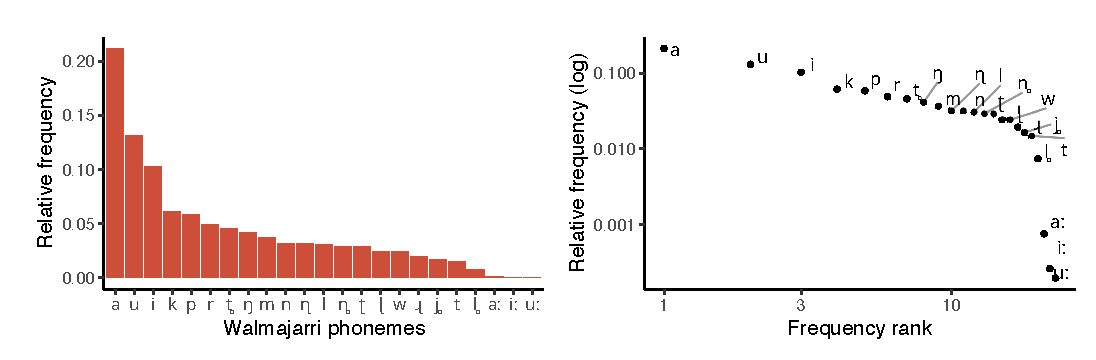
\includegraphics[width=180mm]{03-phoneme-frequencies/fig/Fig1_walmajarri} 

}

\caption[Frequency of phonemes in Walmajarri lexicon \autocite{hudson_walmajarri_1993}]{Frequency of phonemes in Walmajarri lexicon \autocite{hudson_walmajarri_1993}. Plot (A) displays relative frequencies of each segment type. Plot (B) shows the same frequencies on log-transformed \(x\) and \(y\) axes---the traditional visual device used to identify power laws.}\label{fig:Figure-1}
\end{figure}



Phonological frequency data differs in some respects from the data types most commonly encountered in scientific power law studies, such as word frequencies or city populations. Typically, in order to understand a population (and some property of it), such as the cities in the United States (and their sizes), or the words of English (and their frequencies), it is impractical to examine every last member of the population, and so the study will examine a sample. Ensuring that a sample is of sufficient size is an important consideration, firstly in order to adequately represent the population and additionally because a sufficiently large sample size is an important requirement in maximum likelihood estimation \autocites{barndorff-nielsen_inference_1994}{newman_power_2005}. In contrast, the phonemic inventory of any language is relatively small, and it is entirely feasible to examine exhaustive populations of phonemes.\footnote{The probability that we have failed to observe some phoneme that exists in a language is small, though non-zero. In Section S5, Supplementary Materials we evaluate whether this is the case in our data. We find only three languages where it is. Even in such cases, the missing segment inevitably will be an especially low frequency type, and is unlikely to dramatically alter the overall frequency distribution of segments in the language.} An advantage of this is that the sample is highly representative of the population, but a disadvantage is that the number of observations is small and cannot be increased.

Given a sample of phonemes, we require an estimate, or measurement, of their frequencies. Measurement error is a potential concern in this study. Our segment frequencies are calculated from documented wordlists, which necessarily are limited representations of the complete vocabulary of the languages that the wordlists represent. One concern is that the particular morphology of a language's citation forms may cause certain segments in the language to be overrepresented in a wordlist which contains only citation forms. This would represent a bias, that is, a factor that pushes observations in a certain direction. We have attempted to control for this, by removing identifiable citation-form tense morphology from verbal words and noun-class prefixes from nominals. Another source of concern is that wordlists with a smaller number of words will necessarily entail a greater level of uncertainty in the observed segment frequencies. This will be a source of noise in the data. It does not push observed frequencies in any particular direction, but makes them generally less accurate. To address this, in our study, we restrict the language sample to language varieties with a minimum wordlist size of 250 lexical items. We selected 250 lexical items as a cut-off on the basis of \textcite{dockum_swadesh_2019}, who investigate the effect of wordlist size on phonological segment frequencies. \textcite{dockum_swadesh_2019} report accelerating losses in the fidelity of segment frequency estimates as a wordlist drops below 250 items. While more words will always yield better frequency estimates, we select a minimum of 250 as a reasonable compromise. This gives us a sample of 166 Australian language varieties. Wordlist sizes range from 268 to 8742 (median 1072, mean 1438).

\hypertarget{phon-freq-statistical-framework}{%
\subsection{Statistical framework}\label{phon-freq-statistical-framework}}

We test for the presence or absence of a power law in the distributions of phonological segments following the maximum likelihood framework described by \textcite{clauset_power-law_2009}. In brief, Clauset et al.'s \autocite*[p.~663]{clauset_power-law_2009} proposed procedure consists of three steps:

\begin{enumerate}
\def\labelenumi{\arabic{enumi}.}
\item
  Estimate the parameters \(x_{min}\) and \(\alpha\) of the power law model using the maximum likelihood method \autocites{barndorff-nielsen_inference_1994}{newman_power_2005}\footnote{Maximum likelihood estimation (MLE) is a method for estimating the parameters in a statistical model, given some set of observations by finding the set of parameter values, \(\hat{\theta}\), that maximise a likelihood function, \(P(x\ |\ \hat{\theta})\), where \(x\) is a set of observations. In our case, the parameters, \(\hat{\theta}\), to be estimated are those which define a particular distribution---for example, \(\alpha\) and (optionally) \(x_{min}\) in a power law model.}.
\item
  Calculate the goodness-of-fit between the data and the power law using the Kolmogorov--Smirnov (KS) statistic, where a larger value corresponds to a worse fit. Using a Monte Carlo procedure, a \emph{bootstrapped} \(p\) \emph{value} is calculated\footnote{This is a well-established statistical technique. A large number of simulated datasets are created, with data points drawn from the model power law distribution hypothesised in step 1. Each is then fitted to its own power law model and a KS statistic is calculated for the simulated dataset, relative to this model. The \(p\) value is defined as the fraction of these simulated KS distances larger than the actual, observed KS distance.}, and used to evaluate the plausibility of the power law. Namely, if this \(p\) value falls below a plausibility threshold of 0.1, the power law model is rejected.\footnote{Here we follow the method of Clauset, Shalizi, and Newman (2009), who suggest a threshold of 0.1. Note though, that even when p\textgreater{}0.1, we still do not necessarily accept that the power law is a good fit, rather there is a further round of evaluation (step 3). This use of a `\(p\) value' differs from the more common use case where a null hypothesis is rejected when the p value is above a certain level. The reason for the difference lies in how the hypothesis of interest is related to the null hypothesis. Commonly, the hypothesis of interest is set up as the alternative hypothesis, and low p-values are required to reject the null hypothesis (not of interest). Here, the hypothesis of interest (power law is plausible) is set up as the null hypothesis. Accordingly, it too is rejected when the p-value is low. By allowing it to be rejected all the way up to 0.1 (rather than 0.05, for example), we are setting the bar relatively high. This approach may seem counterintuitive in the context of testing a single distribution hypothesis (where it might seem better to make the distribution of interest deliberately harder to accept than to reject). But in the context of testing which distribution fits the data best among multiple alternatives, it makes sense to make it deliberately hard to reject any particular distribution type.} Otherwise, the power law model remains an initially plausible hypothesis, and we proceed to step 3.
\item
  Compare the power law model with a set of models representing alternative hypotheses. For each alternative model, a bootstrapped \(p\) value is calculated as in steps 1 and 2 above. A likelihood ratio test is performed, comparing the fit of the alternatives with those of the power law model. If the calculated likelihood ratio is significantly different from zero, this indicates a significant difference in plausibility, and its sign (positive or negative) indicates which model is favoured \autocite[p.~680]{clauset_power-law_2009}.
\end{enumerate}

We use the \emph{poweRlaw} package \autocite{gillespie_fitting_2014} in \emph{R} \autocite{r-core-team_r_2017} to infer all maximum likelihood estimates and conduct bootstrapping to derive \(p\) values. We run 10,000 bootstrap iterations per language, per distribution type.\footnote{We find that 10,000 iterations are sufficient to obtain stable parameter estimates. Beyond 10,000 iterations, estimates will continue to fluctuate but in a tightly prescribed range. Plots of all bootstrapping runs can be viewed in the interactive visualisation app provided in Section S6.}

As a brief point of comparison to prior work, we return to the Walmajarri example and plot the linear relationship between phoneme frequencies and rank on a log-log plot. \textcite{tambovtsev_phoneme_2007} find that a Zipfian distribution consistently underestimates the frequency of both high- and low-ranking segments while overestimating the frequency of those in the middle. The dashed black slope on Figure \ref{fig:Figure-2} shows a similar pattern. However, when the five lowest-frequency segments (i.e., those with the greatest statistical rank) are removed from the equation, the linear model fits much better (solid blue line). This is consistent with the observation by \textcite{clauset_power-law_2009} that, in practice, power laws are rarely observed across the whole distribution---rather, there is a threshold, the \(x_{min}\) parameter, below which the power law ceases to apply. Visual inspection of other languages in the dataset indicates that Walmajarri's pattern of phoneme frequencies is common, although there is a good deal of variation (and, consequently, variation in the fit of a linear model). However, given the known limitations of applying a linear model to a log-log plot, we now turn to more reliable methods for validating the presence of a power law, using the maximum likelihood method outlined above.

\begin{figure}

{\centering 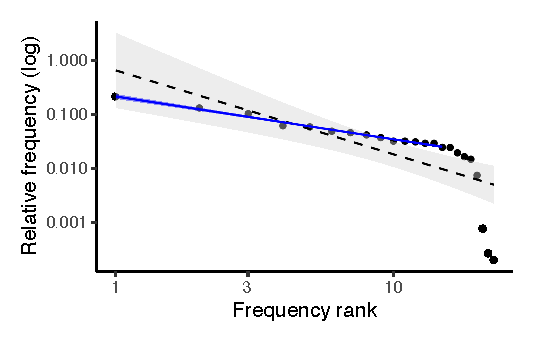
\includegraphics[width=85mm]{03-phoneme-frequencies/fig/Fig2_walmajarri_lm} 

}

\caption[Log-log plot of frequencies versus frequency ranks in Walmajarri]{Log-log plot of frequencies versus frequency ranks in Walmajarri. When a linear model is fitted to the full distribution (dashed black), high and low frequency segments are overestimated and mid-rank segments are underestimated. When lowest-frequency segments are removed from the model (solid blue), the model appears to fit well.}\label{fig:Figure-2}
\end{figure}

\hypertarget{phon-freq-results}{%
\section{Results}\label{phon-freq-results}}

We firstly infer the fit of a power law to the full distribution of phoneme frequencies for each language, without estimating an \(x_{min}\) parameter. In Table \ref{tab:pl-summary} we summarise the maximum likelihood estimates of the power law distribution's defining shape parameter, \(\alpha\), the goodness-of-fit of the estimated power law distribution to the observed distribution of phoneme frequencies, and bootstrapped \(p\) values for the null hypothesis that the data are plausibly drawn from a power law distribution.

\begin{table}

\caption[Power law (without $x_{min}$)]{\label{tab:pl-summary}Power law (without $x_{min}$). Summary of $\alpha$ paramter, goodness-of-fit and $p$ values for the power law distribution fitted to each language's full phonemic inventory.}
\centering
\begin{tabular}[t]{lcccc}
\toprule
\textbf{ } & \textbf{Mean} & \textbf{SD} & \textbf{Min} & \textbf{Max}\\
\midrule
$\alpha$ & 1.38 & 0.17 & 1.16 & 2.18\\
goodness-of-fit & 0.35 & 0.07 & 0.15 & 0.53\\
$p$ & 0.01 & 0.03 & 0.00 & 0.27\\
\bottomrule
\end{tabular}
\end{table}

Mean \(\alpha\) is 1.38 (SD 0.17). As discussed earlier, the standard range of \(\alpha\) is 2 \textless{} \(\alpha\) \textless{} 3 \autocite[p.~662]{clauset_power-law_2009}. \(\alpha\) falls within this range for only 1 language. Furthermore, \(p\) values are very low. Just 2 of the 166 languages give a \(p\) value above the plausibility threshold.

Throughout this study, the possibility of type I error (false positives) must be taken into consideration. By setting our implausibility range at \(p \leq\) 0.1, we accept a one in ten chance of incorrectly rejecting a power law hypothesis which in fact is plausible---this can occur when the distribution's poor fit is due to chance fluctuation alone. Given 166 tests (one test per language), we would therefore expect to reject \(H_0\) incorrectly in around 17 (10\%) of those tests. In this instance though, we have rejected \(H_0\) as implausible in 99\% of the language sample. Thus it is clear that the power law distribution is being deemed implausible not merely by chance. It is genuinely a poor fit for the vast majority of languages. This result accords well with earlier work which has found that a simple, one-parameter form of the power law distribution poorly characterises phoneme frequencies \autocites{sigurd_rank-frequency_1968}{martindale_comparison_1996}{tambovtsev_phoneme_2007}.

As discussed earlier, our dataset of phoneme frequencies is very likely to contain the complete population of phonemes in each language. At the same time, the number of observations per language is low---ranging from 16 to 37 segments in our language sample (mean 24.5, SD 3.8). Such a small set of observations can be a barrier to highly accurate maximum likelihood estimation. \textcite[p.~669]{clauset_power-law_2009} suggest that a minimum sample size of around 50 is needed to get a maximum likelihood estimate of \(\alpha\) accurate to at least 1\%. This is simply not possible for most of the world's languages (including all languages in this study) due to the limited size of segment inventories. Thus, in phonemic studies such as ours there is likely to be an unavoidable uncertainty in the estimate of \(\alpha\).

\hypertarget{power-law-xmin-results}{%
\subsection{\texorpdfstring{Power law distribution with \(x_{min}\)}{Power law distribution with x\_\{min\}}}\label{power-law-xmin-results}}

If the power law distribution, as inferred above, is inadequate for characterising phoneme frequencies, then what other options are there? There are a couple of approaches to this question. One is to add an additional parameter to improve the fit of the power law; the other is to consider alternative distribution types. In this and the following sections we explore both approaches.

Here, we infer the fit of a power law distribution with an additional \(x_{min}\) parameter, whose effect is to remove some of the least-frequent observations from the sample which is being fitted. As above, we use maximum likelihood to infer the best-fitting \(x_{min}\) threshold for each language. Results are summarised in Table \ref{tab:pl-xmin-summary}.

\begin{table}

\caption[Power law distribution (with $x_{min}$)]{\label{tab:pl-xmin-summary}Power law distribution (with $x_{min}$). Summary of $\alpha$ paramter, goodness-of-fit and $p$ values for the power law distribution fitted to a subset of more frequent phonemes in each language.}
\centering
\begin{tabular}[t]{lcccc}
\toprule
\textbf{ } & \textbf{Mean} & \textbf{SD} & \textbf{Min} & \textbf{Max}\\
\midrule
$\alpha$ & 2.75 & 0.65 & 1.51 & 6.14\\
goodness-of-fit & 0.14 & 0.03 & 0.08 & 0.22\\
$p$ & 0.62 & 0.26 & 0.01 & 1.00\\
\bottomrule
\end{tabular}
\end{table}

After inferring an \(x_{min}\) parameter, the power law distribution is fitted to an average of only 13.9 segments, though there is a wide degree of variation (SD 4.1). In percentage terms, the power law distribution is fitted to an average of 57\% of a language's segmental inventory (SD 16\%). 117 languages (70\%) fall within the normal 2--3 range for \(\alpha\). Having only a small number of included observations above the \(x_{min}\) threshold can drive unreasonably high estimates of the \(\alpha\) scaling parameter. A sizeable portion of our sample (43 languages, 26\%) fall in this high range with \(\alpha\) above 3. At the other extreme, 6 languages (4\%) have an unusually low \(\alpha\) under 2. Mean \(\alpha\) is 2.75 (SD 0.65).

When \(x_{min}\) is included, the power law hypothesis is accepted as plausible (though, to emphasise, not necessarily correct) in the 158 of 166 language varieties for which \(p >\) 0.1. \(p\) falls below the 0.1 plausibility threshold in the remaining 8 languages. The lowest \(p\) value for any language is 0.011. This puts the chance of incorrectly rejecting \(H_0\) at around 1 in 100. The likelihood of a 1-in-100 event is high in a set of 166 tests. Overall, since the number of \(p\) values below 0.1 is considerably fewer than the number we would expect to observe through chance, and since there is a reasonable possibility that the lowest \(p\) value, 0.011, is a type I error, we cannot confidently rule out the power law hypothesis for any language in our sample.

Although we have failed to rule out the power law distribution as implausible for any specific language, this still does not mean that the power law distribution is the optimal one for our data, and there are some important caveats to our results so far.

A distribution will always fit a set of data at least as well as the same distribution with one fewer parameter. Thus, the observation that the power law distribution fits better when \(x_{min}\) is added requires some interpretation. Of greatest interest in this respect is the striking degree of improvement in fit, such that the power law distribution shifts from a largely implausible fit against full phoneme inventories, to a largely plausible fit after we exclude the least-frequent observations from samples. This raises the obvious question of why this might be so. We consider this in our Discussion, after we have also examined distributional alternatives to power laws.

The inclusion of an \(x_{min}\) parameter when fitting power laws is common practice, but its use is most obviously motivated in contexts where there are very many possible observations. For example, Clauset et al. \autocite*[p.~684]{clauset_power-law_2009} fit a power law to frequencies of unique words in Moby Dick and find a best-fitting \(x_{min}\) of 7 (\(\pm2\)). Words occurring fewer than 7 times can be disregarded and this still leaves nearly 3,000 unique words to which the power law distribution can be fitted. In contrast to this typical use case, where a large number of observations remain in play and do fit the power law, our use of \(x_{min}\) with phoneme datasets results in the exclusion of data points from an already small sample, leaving an even smaller set of data being fitted. As a general fact, it is inherently difficult to identify the most appropriate distribution for a small collection of observations. Correspondingly, it is not automatically an insightful finding, that a power law can be plausibly fitted to such small datasets. However, as mentioned just above, it is noteworthy that the same power law did not fit well to the slightly larger datasets that were being used without the \(x_{min}\) parameter. This suggests that it is not the merely small size of the dataset which is causing the good plausibility of the fit.

Small samples of observations can inflate \(p\) values, as is the case when investigating phonemes. We have good reason to suspect our \(p\) values are being inflated by the low number of observations per language, the evidence being that the number of \(p\) values we observe below 0.1 is considerably fewer than we would expect by chance. The difficulty we find in ruling out the power law distribution may reflect this.

\hypertarget{alternative-distributions}{%
\subsection{Alternative distributions}\label{alternative-distributions}}

In addition to considering the merits of adding extra parameters to a distribution, we must also consider whether a completely different distribution would provide an equally good or better fit to the data. We consider three alternative distributions, which are not part of the power law family and may suggest different underlying generative processes. These are the lognormal, exponential and Poisson distributions. Like the power law distribution, the shape of these distributions can have a sharp initial peak and a rapidly decaying tail, as illustrated in Figure \ref{fig:Figure-3}.

\begin{figure}

{\centering 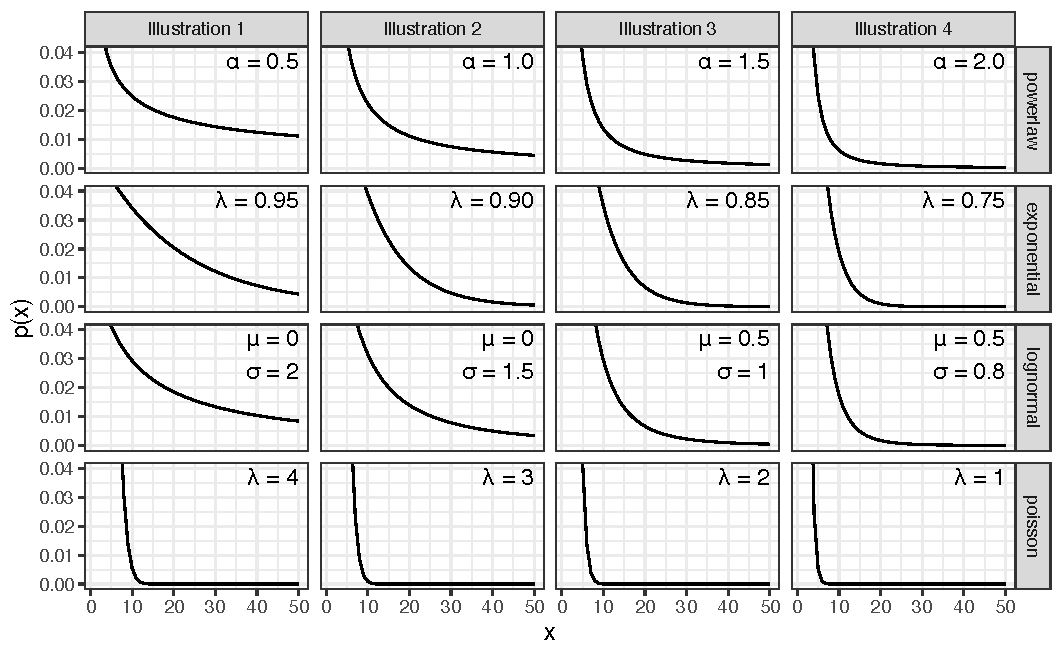
\includegraphics[width=180mm]{03-phoneme-frequencies/fig/Fig3_distribution_illustrations} 

}

\caption[Illustrations of power law, exponential, lognormal and Poisson distributions]{Four distribution types: power law, exponential, lognormal and Poisson, each illustrated with four parameterisations.}\label{fig:Figure-3}
\end{figure}

\hypertarget{lognormal-distribution}{%
\subsection{Lognormal distribution}\label{lognormal-distribution}}

The lognormal distribution is one where the data form a normal distribution when transformed on a log scale. Once again, we use the \emph{poweRlaw} package \autocite{gillespie_fitting_2014} to estimate parameter values using maximum likelihood. In this instance, the parameters to be estimated are log mean and log standard deviation parameters---the log-scale equivalent of the two parameters that define a normal distribution. We fit the distribution to the whole set of segment frequencies for each language---we do not estimate an \(x_{min}\) parameter at this stage (though see below). The lognormal distribution narrowly construed is a continuous distribution, however the \emph{poweRlaw} package contains a corresponding discretised version, appropriate to phoneme frequency data.

As for the power laws above, we calculate bootstrapped \(p\) values to assess the plausibility of the fit of the lognormal distribution for each language. The \(p\) values obtained are highly variable throughout the dataset. There are 73 languages (44\% of the language sample) for which \(p\) falls in the range of implausibility, below 0.1. This is higher than we would expect if the lognormal distribution were plausible for all languages and \(p \leq\) 0.1 values were due to type I error alone. This result is a little difficult to interpret, given the previously discussed difficulties with small samples of observations per language. What seems clear is that, given the rate of \(p \leq\) 0.1 values is elevated beyond chance, we cannot say that the lognormal distribution plausibly characterises the segment frequencies of all languages. Nevertheless, for many languages---56\% of languages in our sample---we cannot confidently rule out the lognormal distribution. Overall, this makes the lognormal distribution with no \(x_{min}\) a better fit than the power law distribution with no \(x_{min}\), which we ruled out for up to 99\% of languages in the sample. One caveat to keep in mind is that the lognormal distribution is minimally defined by two parameters rather than one, which potentially puts it at an advantage compared to the single-parameter power law distribution.

\hypertarget{exponential-distribution}{%
\subsection{Exponential distribution}\label{exponential-distribution}}

An exponential distribution, and its discrete analogue, a geometric distribution, is one in which frequencies decay at a constant proportional rate. Thus for the frequencies of any two successively-ranked phonemes, \(x_k\) and \(x_{k+1}\), the distribution is characterised by a rate parameter, \(\lambda\), so that \(x_{k+1} = \lambda.x_k\). Here, as above, we use maximum likelihood to estimate the parameter \(\lambda\) and the bootstrapping procedure to obtain a \(p\) value.\footnote{This generates a relationship where \(p(x_k) \propto \lambda^k\). An alternative expression of the same relationship is \(p(x_k) \propto e^{-\lambda' k}\), where \(\lambda' = -log(\lambda)\). Results reported in Sections S5 and S6 of the Supplementary Material use this second definition, with \(\lambda'\).}

Bootstrapped \(p\) values are above the 0.1 plausibility threshold for 147 of 166 languages. The number of languages for which \(p \leq\) 0.1 is 19, close to the 17 or so that we would expect from type I errors. This, on the face of it, seems to make the exponential distribution quite a plausible model for phonological segment frequencies more generally. It must be noted, however, that there are a few languages for which the exponential distribution is a very poor fit. The most extreme, Miriwoong, has a goodness-of-fit statistic of 0.27 and a \(p\) value of 0.036. The poor quality of fit is visually evident on a log-log plot (see Section S6, Supplementary Materials).

\hypertarget{poisson-distribution}{%
\subsection{Poisson distribution}\label{poisson-distribution}}

The final distribution we consider is the Poisson distribution, which is related to the exponential distribution. The Poisson distribution is typically used to model the frequency of an event within some interval of time or space. Our case is a bit different since we are modelling the relationship between the frequency of many different events (different phonological segments) and their frequency rank in a language's phonological inventory. As with the exponential distribution, we use maximum likelihood to estimate a single parameter, \(\lambda\), and use bootstrapping to obtain a \(p\) value for the plausibility of the distribution.

The Poisson distribution is totally implausible for all languages in our language sample. Goodness-of-fit statistics range from 0.43 to 0.75 (mean 0.59, SD 0.07). We find \(p\) values indistinguishable from 0 in all cases.

\hypertarget{phon-freq-results-summary}{%
\subsection{Summary of results by individual distribution type}\label{phon-freq-results-summary}}

In Table \ref{tab:results-summary}, we summarise results for the four distribution types evaluated in this study. For each distribution type, we give the number of languages for which the distribution's fit was deemed plausible (\(p >\) 0.1). For completeness, we give results for the exponential, lognormal and Poisson distributions when \(x_{min}\) is included, just as we did for the power law distribution. (Note: for one language, the bootstrapped \(p\) value estimation procedure failed to converge for the lognormal distribution with \(x_{min}\). This is the only distribution we tested which has three free parameters, and in this instance, the algorithmic procedure struggles to differentiate solutions with very similar likelihoods.) Perhaps most noteworthy among these results is the greatly increased inconclusiveness of the method when applied to the reduced set of data points lying above the \(x_{min}\) threshold. When the fitting task is restricted to a subset of only the most frequent segments in a language, it is possible to plausibly fit all but the Poisson distribution to any language, after type I error is factored in. One difference, which we nuance further in the next section, is that power law distributions with \(x_{min}\) are fitted on average to only 57\% of a language's phonemes, whereas the lognormal and exponential distributions are fitted to closer to 80\%.

\begin{table}

\caption[Results summary]{\label{tab:results-summary}Results summary. For each of the four distributions considered, this table lists the number of languages (and percentage of the total language sample) for which the distribution plausibly fits, as indicated by an uncorrected $p > 0.1$ value. 'Prop. fitted' gives the average proportion of each language's phoneme inventory above $x_{min}$.}
\centering
\begin{tabular}[t]{lccc}
\toprule
\textbf{ } & \textbf{Without $x_{min}$} & \textbf{With $x_{min}$} & \textbf{Prop. fitted}\\
\midrule
Power law & 2 (1\%) & 158 (95\%) & 56\%\\
Lognormal & 93 (56\%) & 155 (93\%) & 78\%\\
Exponential & 147 (89\%) & 146 (88\%) & 84\%\\
Poisson & 0 (0\%) & 43 (26\%) & 17\%\\
\bottomrule
\end{tabular}
\end{table}

\hypertarget{evaluation-of-comparative-best-fit}{%
\subsection{Evaluation of comparative best fit}\label{evaluation-of-comparative-best-fit}}

The third and final step in Clauset \emph{et al.}'s \autocite*{clauset_power-law_2009} framework is a likelihood ratio test. This third step may not always be necessary. If the bootstrapping procedure, above, were to show that only one distribution type plausibly fits the data, it would already have been shown to have the best fit among the candidates examined. However, bootstrapping may identify multiple distribution types as plausible. It will be recalled that just because a distribution is judged plausible via the bootstrapping process does not mean that it is the optimal one, since there may be other equally or more plausible distributions. Accordingly, when there are multiple plausible candidate distributions, \textcite{clauset_power-law_2009} recommend using Vuong's \autocite*{vuong_likelihood_1989} likelihood ratio test for model selection, to determine the best-fitting of any pair of competing models. Full results of all likelihood ratio tests described in this section are tabled in Section S5 of the Supplementary Materials.

Vuong's \autocite*{vuong_likelihood_1989} test uses the Kullback-Leibler Information Criterion \autocite{kullback_information_1951} to calculate the log likelihood of observing the data given a distribution model, and compares this to the log likelihood of observing the same data given a competing distribution model. The test returns a test statistic, which gives an indication of how strongly one model is favoured over another, and a \(p\) value, indicating whether the difference in the support for each model is statistically significant.

We begin by comparing distributions without the \(x_{min}\) parameter. As summarised in Table \ref{tab:results-summary}, two of these distributions (the power law and Poisson distributions, without \(x_{min}\)) have already been rejected as implausible for all or nearly all languages. Accordingly, we conduct just one likelihood ratio test per language, comparing the fit of the exponential versus lognormal distributions. Overall, we find that Vuong's likelihood ratio test somewhat favours the exponential distribution. Likelihood ratios favour the exponential distribution for 122 languages, and the lognormal distribution for 44 languages. However after Bonferroni correction, the difference in the likelihood of exponential and lognormal models is statistically significant for only two languages, Thaynakwithi and Dalabon, both favouring the exponential distribution.

Turning to distributions with the \(x_{min}\) parameter, since we have already rejected the Poisson distribution, we conduct likelihood ratio tests pairwise among the remaining three distributions. In order to compare distributions with \(x_{min}\) parameters, it is necessary to set \(x_{min}\) to the same value in both distributions \autocite{gillespie_fitting_2014}. Thus, to make a pairwise comparison, we take the \(x_{min}\) value from distribution A and using it, re-estimate the other parameters of distribution B, and conduct one likelihood ratio test. Then we take \(x_{min}\) from B, use it and re-estimate the other parameters of distribution A, and conduct a second likelihood ratio test, giving two results for each pair of distributions.

Comparing the exponential and lognormal distributions, the likelihood ratios favour the lognormal distribution (139 languages to 27) using \(x_{min}\) from the lognormal fit, and favours the exponential distribution (103 languages to 63) using \(x_{min}\) from the exponential fit, however none of these comparisons reaches significance after Bonferroni correction.

Comparing the power law and lognormal distributions, likelihood ratios favour the lognormal distribution (144 languages to 22) using \(x_{min}\) from the power law fit, and all languages when using \(x_{min}\) from the lognormal fit, however only two of these comparisons reaches significance after Bonferroni correction. Yir Yoront favours the power law when using \(x_{min}\) from the power law fit and Malyangapa favours the lognormal distribution using \(x_{min}\) from the lognormal.

Comparing the power law and exponential distributions, the likelihood ratios favour the power law (133 languages to 33) when taking \(x_{min}\) from the power law fit, though no comparison reaches significance. They favour the exponential distribution 164 languages to 2 when \(x_{min}\) is taken from the exponential fit. Thirteen of those comparisons reach significance.

In sum, we found earlier that when parameterised without \(x_{min}\), only the exponential and lognormal distributions were broadly plausible. Voung's likelihood ratio test marginally favours the exponential test over the lognormal when fitted against entire phonemic inventories, but the difference is at most slight. When parameterised with \(x_{min}\), the power law distribution is fitted to around 60\% of languages' phonemes on average, while the exponential and lognormal are fitted to around 80\% (Table \ref{tab:results-summary}). Pairwise likelihood ratio tests, which apply one distribution's \(x_{min}\) parameter to the other, provide slender evidence of the following. Even when fitted against the small phonemic subsets favoured by the power law, the lognormal distribution may weakly outperform the power law, but the exponential distribution does not. Fitted against the larger subsets favoured by the exponential and lognormal distributions, the power law is outperformed by the exponential and lognormal. The performance of the latter two distributions is indistinguishable.

\hypertarget{phon-freq-discussion}{%
\section{Discussion}\label{phon-freq-discussion}}

Here we contextualise the current study more fully in the history of research into power laws and phoneme frequencies, before drawing implications and conclusions from the new findings we have obtained.

\hypertarget{power-laws-linguistics}{%
\subsection{Power laws in linguistics}\label{power-laws-linguistics}}

Investigation of power laws in the linguistic sphere has a long history. One of the oldest and best-known examples of a power law in any discipline is the distribution of word frequencies in text corpora, first noted by \textcite{estoup_gammes_1916} and subsequently described by Zipf \autocites*{zipf_selective_1932}{zipf_human_1949}. Zipf's Law, as it has come to be known, is a discrete power law distribution. Its exponent parameter, \(\alpha\), is typically very close to 1, in which case, the second ranked item will be approximately half as frequent as the first, the third ranked item will be one third as frequent as the first, and so on. Zipf's Law continues to garner considerable attention, for example in \textcite{kucera_computational_1967}, \textcite{montemurro_beyond_2001}, and more recently in Baayen \autocites*{baayen_word_2001}{baayen_analyzing_2008}. Various modifications to Zipf's formula have been suggested \autocite[notably][]{mandelbrot_structure_1954} and theoretical explanations put forward \autocites{li_random_1992}{naranan_information_1992}{naranan_models_1998}.

Power laws have also been proposed to describe the distribution of phoneme frequencies. The use of Zipf's Law to model the frequencies of phonological segments initially appears to be an attractive prospect \autocite[pp.~565--566]{witten_source_1990}. Nevertheless, a selection of alternative, non-power law distributions has also been suggested.

\textcite{sigurd_rank-frequency_1968} is an early study evaluating the fit of a Zipfian distribution to phoneme frequencies, where the exponent, \(\alpha\), is set to 1. His evaluation method is a simple visual inspection, comparing observed phoneme frequencies in five languages (selected for their variety in segmental inventory size) with their expected frequencies assuming a Zipfian rank-frequency relationship. \textcite[p.~8]{sigurd_rank-frequency_1968} observes that the phoneme frequency distributions do not approximate a Zipfian curve, particularly for the most common segments. Rather, \textcite{sigurd_rank-frequency_1968} finds better approximations using a geometric series equation, so that \(x_{k+1} = \lambda.x_k\) for some rate parameter \(\lambda\), giving the discrete distribution:

\begin{equation}
p(x_k) \propto \lambda^k
\label{eq:sigurds-geometric}
\end{equation}

\textcite[p.577]{good_statistics_1969} suggests an alternative method of approximation: following \textcite{whitworth_choice_1901}, Good calculates the expected frequencies of each phoneme given a process whereby a unit interval probability space \([0,1]\) is divided into \(n\) parts at random (where \(n\) is the number of phonemes in the language), following a uniform distribution. This is equivalent to a so-called stick-breaking process: imagine a stick, which represents the unit interval probability space. The stick is broken into \(n\) parts; the \(n-1\) places along the stick at which a break is made are selected randomly and all at once, with any place along the stick equally likely to be selected as any other. When these parts are rearranged by size, from smallest to largest, their expectation follows the distribution:

\begin{equation}
\frac{1}{n^2},\quad \frac{1}{n} \left( \frac{1}{n} + \frac{1}{n-1} \right),\quad \frac{1}{n} \left( \frac{1}{n} + \frac{1}{n-1} + \frac{1}{n-2} \right),\quad ...
\label{eq:whitworth-dist}
\end{equation}

Which is to say:

\begin{equation}
p(x_k) \propto \sum_{i=k}^{n} \frac{1}{i}, \quad 1 \leq k \leq n
\label{eq:whitworth-rank-dist}
\end{equation}

In support of this model, \textcite[p.577]{good_statistics_1969} provides a table of observed versus expected frequencies of both graphemes and phonemes in English, however the sample size is modest (1000 words) and does not extend to any other languages. Furthermore, there is no visual or statistical evaluation of the goodness-of-fit. \textcite{good_statistics_1969} intends for the results to be taken as a curious observation only, with no strong theoretical position or claim of generalisability.

As \(n\) in equation \eqref{eq:whitworth-rank-dist} grows large, the summation term \(\sum_{i=k}^{n} \frac{1}{i}\) converges towards \(-log(\frac{k}{n+1})\) \autocite[p.~12]{loeb1989formal}, meaning that Good's distribution can be considered an approximation of \eqref{eq:borodovsky-rank-dist}, a discretised negative logarithmic distribution.

\begin{equation}
p(x_k) \propto -\log \frac{k}{n+1}, \quad 1 \leq k \leq n
\label{eq:borodovsky-rank-dist}
\end{equation}

\textcite{gusein-zade_distribution_1988} and \textcite{borodovsky_general_1989} visually evaluate the fit of \eqref{eq:borodovsky-rank-dist} to the graphemes of English, Estonian, Russian and Spanish.\footnote{Of course, the statistics of graphemes are different from the statistics of phonological segments. As \textcite[pp.~136--137]{bloomfield_language_1935} rather emphatically points out: ``If we take a large body of speech, we can count out the relative frequencies of phonemes and of combinations of phonemes. This task has been neglected by linguists and very imperfectly performed by amateurs, who confuse phonemes with printed letters.'' Nevertheless, the frequencies of graphemes has been of interest historically in many applications; for example, in traditional printing, the development of Morse code, and library cataloguing \autocite[pp.~550--551]{witten_source_1990}.} They also use the equation to describe the distribution of DNA codons \autocite{borodovsky_general_1989}. \textcite[pp.~563--566]{witten_source_1990} examine the frequencies of single graphemes, graphemic bigrams and trigrams in the Brown Corpus and compare the fits of Good's distribution and Zipf's Law by comparing expected entropy values for each model to observed entropy scores. They find that the quality of the fit of Good's model declines with bigrams and trigrams compared to single graphemes, although the observed distribution curves are broadly of the same shape (and resemble the shape of Good's distribution rather than the Zipfian distribution). When assessed using metrics based on entropy, Good's distribution fits better than or around equally as well as the Zipfian distribution for all three datasets. Good's distribution and the negative logarithmic distribution it approximates also have the advantage of parsimony, since they are parameter-free: knowing how many unique items (phonemes, graphemes, bigrams, etc.), \(n\), are in the dataset is sufficient to calculate their expected distribution of frequencies---there are no additional parameters to estimate such as \(\alpha\) in \eqref{eq:zipfs-law} or \(\lambda\) in \eqref{eq:sigurds-geometric}.

\textcite{martindale_comparison_1996} compare the fit of four different distributions to frequencies of both graphemes and phonemes in text corpora from 18 languages. Using the \(R^2\) statistic in a linear regression, they compare the fit of the parameter-free negative logarithmic equation of \textcite{borodovsky_general_1989} in \eqref{eq:borodovsky-rank-dist} to the Zipfian power-law distribution \eqref{eq:zipfs-law}, Sigurd's geometric series distribution \eqref{eq:sigurds-geometric}, and the Yule-Simon distribution \autocites{yule_mathematical_1925}{simon_class_1955}, which can be written:

\begin{equation}
p(x_k) \propto \frac{1}{k^\alpha}.\lambda^k
\label{eq:yule}
\end{equation}

The Yule-Simon equation in \eqref{eq:yule} is the product of the power law in \eqref{eq:zipfs-law} and the geometric equation in \eqref{eq:sigurds-geometric}. Because of the differing rates at which the two parts of the equation decay as \(k\) increases, equation \eqref{eq:yule} produces a distribution which is more like a power law \eqref{eq:zipfs-law} for low values of \(k\) (and thus for high frequency items, for instance) and more like the geometric \eqref{eq:sigurds-geometric} for high values of \(k\) (low frequency items) \autocite{simon_class_1955}.

The Yule-Simon equation in \eqref{eq:yule} has not just one free parameter but two, the exponent \(\alpha\) and the rate \(\lambda\), and the Zipfian and Sigurd equations are effectively special cases of it, each with one parameter fewer. The Zipfian distribution is equivalent to \eqref{eq:yule} with \(\lambda\) set to 1 (so that \(\lambda^k = 1\)), while the geometric equation is equivalent to \eqref{eq:yule} with \(\alpha\) set to zero (so that \(1/k^\alpha = 1\)). This is important, since as a general fact, if distribution A is a special case of distribution B, with fewer free parameters than it, then B will always perform at least as well as A when fitting the same set of data. Thus, the Yule-Simon distribution will necessarily fit the same set of data at least as well as the Zipfian distribution, and Sigurd's geometric distribution.

\textcite{martindale_comparison_1996} find that the Yule-Simon distribution fits best, for both graphemes and phonemes. They find that the Zipfian distribution tends to overestimate both high and low frequency items, although the differences they observe between models are only small. On this basis, they conclude that it is ``a matter of taste'' whether one opts for the more precise Yule-Simon distribution or simpler models with fewer parameters to estimate \autocite[p.~111]{martindale_comparison_1996}. \textcite{tambovtsev_phoneme_2007} expand Martindale et al.'s \autocite*{martindale_comparison_1996} study to include phoneme frequencies in 95 languages (90 of these are Eurasian; 2 are from Oceania and 1 each from Australia, Africa and South America). The sample is divided into four language groups (Indo-European, Altaic and Yukaghir-Uralic--plus a miscellaneous group) and a series of pairwise sign tests are conducted to test whether the difference in mean \(R^2\) is significant between different distributions for each language group. Again, they find that the Yule-Simon distribution fits best overall.\footnote{Although in their statistical tests they do not adjust their significance levels to correct for multiple hypothesis testing.}

Obtaining a better fit by using a distribution with an additional parameter may be relatively trivial mathematically speaking, but this does not mean it is uninteresting. The extra parameter may work to capture a significant real-world nuance in an underlying causal process or describe the effect of one or more secondary processes. A compelling causal explanation of a complex distribution might therefore be formulated by identifying some real-world factor and explaining how its mathematical effect on the distribution is expected to match what we find. It is also important to consider the possibility of equifinality---the fact that multiple, different real-world phenomena may have equivalent mathematical effects. Tests of goodness-of-fit examine only the mathematical aspect, and cannot distinguish between different phenomena whose detectable mathematical contribution is equivalent.

\textcite[p.~111]{martindale_comparison_1996} and \textcite[p.~9]{tambovtsev_phoneme_2007} note that a Zipfian distribution describes frequencies of phonological segments less well than it describes frequencies of words, in part because the highest-frequency phonemes are not frequent enough. They speculate that this may be so, because if the most-frequent phonemes did pattern in a Zipfian way, then perception problems could arise for language users owing to the small size of a phonological inventory. This speculation does not meet the criteria for a compelling causal explanation though. It is not clarified what the linguistic mechanism is, that acts to prevent such perceptual problems, and thus we do not have a real-world phenomenon whose mathematical properties could be interrogated. Nor is it explained why, if such a mechanism exists, its mathematical effect would be to contribute something like the extra geometric term \(\lambda^k\) that differentiates the Yule-Simon distribution \eqref{eq:yule} from the Zipfian \eqref{eq:zipfs-law}.\footnote{The Yule-Simon equation, which \textcite{martindale_comparison_1996} and \textcite{tambovtsev_phoneme_2007} find to be a superior fit, describes a distribution which is most similar to a power law for high frequency (low \(k\)) items, and most like the geometric for low frequency (high \(k\)). The claim that its superior fit is due to \emph{non}-power-law-like behaviour of high frequency items is therefore hard to reconcile with the mathematics.} This is not to say that an explanation in terms of perceptibility and confusability is implausible, but rather if our aim is for causal hypotheses that can be evaluated, then more steps are needed, a topic that we return to below. Next, however, we consider the history of investigation presented here, together with our new results.

\hypertarget{findings-from-a-more-reliable-evaluation-procedure}{%
\subsection{Findings from a more reliable evaluation procedure}\label{findings-from-a-more-reliable-evaluation-procedure}}

Power laws have attracted wide and sustained scientific interest. Recent debates on their validity have prompted the development and widespread adoption of novel evaluation methods that are more reliable than those used in the past \autocites{clauset_power-law_2009}{stumpf_critical_2012}. In this study, we re-evaluated the plausibility of several distribution types as characterisations of phoneme frequencies using a maximum likelihood statistical framework presented by \textcite{clauset_power-law_2009} and a sample of 166 Australian language varieties.

Using a more reliable evaluation procedure than previous investigations, we have confirmed the finding that a basic power law distribution, with a single free parameter, is generally insufficient for characterising phoneme frequencies. Additionally, we reconfirm a result going back to \textcite{sigurd_rank-frequency_1968}, that an exponential (or geometric) distribution, with a single free parameter, is a good plausible fit for full phonemic inventories. Furthermore, we find that a lognormal distribution, with two free parameters, is an additional plausible fit, whereas a Poisson distribution, with a single free parameter, is implausible. We did not attempt to fit the two-parameter Yule-Simon distribution in \eqref{eq:yule}, since to our knowledge, there is no maximum likelihood estimation procedure currently available for estimating its parameters. However, we do return to the question of this distribution just below.

A second novel contribution was to consider the addition of an \(x_{min}\) parameter, a practice which is now common in power law research. Notably, while power laws are largely implausible fits for entire phoneme inventories, their plausibility is improved strikingly once a subset of the least-frequent phonemes is removed from the sample. This is despite that fact that the full inventories and the reduced ones share the property of comprising notably small samples. The subset removed in order to achieve maximum likelihood is on average large, at 43\%. This result indicates that power laws constitute a plausible characterisation for the more-frequent portion of phonemic inventories, and explains why the upper end of a Yule-Simon distribution, which most closely approximates a power law, should be a reasonable fit. We note however, that the lognormal distribution also performs well in this same, high frequency region of phonemic inventories. Exponential (or geometric) distributions do not fit the higher-frequency portion of inventories as well the power law or lognormal do, but they are good fits for entire inventories, suggesting that they fit particularly well in lower-frequency portions. This would explain why the lower end of a Yule-Simon distribution, which most closely approximates a geometric distribution, should be a reasonable fit.

Using an evaluation procedure which has since been shown to be unreliable, \textcite{martindale_comparison_1996} and \textcite{tambovtsev_phoneme_2007} concluded that the two-parameter Yule-Simon distribution fit whole inventories better than a power law or a geometric distribution. Implicitly, this is a conclusion in two parts: more-frequent phonemes are more power-law-like, and less-frequent are more geometric-like. Here we have not been able to directly evaluate the Yule-Simon distribution using the more reliable, maximum likelihood method. However, we have found evidence supporting a similar conclusion, that the more-frequent and less-frequent portions of phonemic inventories are characterised by different distributional properties. The more-frequent portion better matches a power law, though also a lognormal distribution. The less-frequent portion better matches a geometric distribution. These two findings serve to clarify and qualify the two implicit halves of the main finding of \textcite{martindale_comparison_1996} and \textcite{tambovtsev_phoneme_2007}, and here we have arrived at them by more reliable methods. Furthermore, by estimating \(x_{min}\) parameters, we have provided some estimates of where power-law-like behaviour starts to cut out within a phonemic inventory. To understand what these results entail for theory, we return to the question of causal processes.

\hypertarget{distributions-outcomes-of-stochastic-processes-linked-to-causal-factors}{%
\subsection{Distributions: outcomes of stochastic processes linked to causal factors}\label{distributions-outcomes-of-stochastic-processes-linked-to-causal-factors}}

Ultimately, linguistic theory seeks to explain the patterns that can be observed in human language. This endeavour will be aided by a sound knowledge of which mathematical distributions plausibly characterise a given variable \(x\) (such as phoneme frequency), since those distributions will be consistent with only certain mathematical kinds of underlying processes. In this paper, we have improved the certainty of our understanding of observed distributions of phoneme frequencies, using state-of-the-art statistical methods. This is a necessary step, but a first step only. A fruitful next step used widely in other sciences is to explicitly consider mathematical families of stochastic processes, whose signature outcome distributions are consistent with those of our empirical observations, and then to ask in turn, what plausible, real-world causal processes could be consistent with these observation-matching stochastic processes.

It can be emphasised that in this model of progress, a good understanding of families of stochastic processes will play an important, enabling role. Accordingly, it will be useful to harness advances that have already been made elsewhere. For instance, many discrete systems can be profitably conceptualised in terms of urn processes with characteristically associated distributions. As \textcite[p.~87]{kuba2012limiting} remark, ``{[}u{]}rn models are simple, useful mathematical tools for describing many evolutionary processes in diverse fields of application''. There exist well-studied urn processes which yield many kinds of distributions. It will be profitable in linguistic research to more clearly relate our own theories of change, including change in phonemic inventories, to these mathematically more generalised processes. By doing so, linguists will be able to tap into related, existing mathematical results (such as relating processes to distributions), that can assist us to further differentiate the theories that are more viable from those that are less so.

\hypertarget{casual-processes-of-phoneme-addition-removal-and-redistribution}{%
\subsection{Casual processes of phoneme addition, removal and redistribution}\label{casual-processes-of-phoneme-addition-removal-and-redistribution}}

Naturally, any observation-matching families of stochastic processes will still need to be related to linguistically plausible causal processes \autocite{cysouw_probability_2009}. Though our paper has primarily focused on methods that will strengthen future discussions around links between observations and causal mechanisms, rather than the causal mechanisms themselves, here we offer some brief remarks on historical mechanisms affecting phoneme frequencies. As we do, we continue using the imagery of urns to represent phonemes types; the balls in them to represent their tokens in the lexicon; and processes that serve to add, remove and redistribute them. \autocite[For a like-minded review of potential mechanisms behind Zipf's law in the frequencies of \emph{words}, see][]{piantadosi2014zipf}

Phoneme frequencies undergo constant modification due to changes occurring at multiple levels of linguistic structure, including the phonology proper, morphology, syntax and the grammar of discourse. Within the phonology itself, fundamental changes include deletions, insertions and changes of phonemic category, all of which will impact phoneme frequency distributions. In an urn model, historical deletions will result in balls being removed from a phoneme's corresponding urn while insertions will add balls. Adding a level of complexity, many phonological changes affect not just one phoneme category, but natural classes of sounds, thus deletions and insertions that apply to natural classes will remove or add balls simultaneously from a non-random, `natural' set of urns.

Phonemic mergers \autocite{hoenigswald1965language} are changes which collapse two erstwhile phoneme categories into one, effectively emptying all balls from one urn into another. Phonemic partial mergers, also known as primary splits, shift only some of a phoneme's instances into another, existing phonemic category, transferring some portion of an urn's balls to another. Phonemic (secondary) splits involve an existing phonemic category splitting into multiple new categories, entailing the creation of one or more new urns, filled with some proportion of the balls from an existing urn, which itself remains non-empty. In both mergers and splits, natural classes may be involved, entailing simultaneous transfers between, and creation or loss of, `natural' sets of urns.

A phonemic category will map onto multiple actual speech sounds, or phones, and the phonemic categorisation of a phone frequently depends on its contextual environment. Consequently, it is not uncommon for multiple types of phonemic changes to occur at once, owing to the fact that when one sound changes, so too does the contextual environment of its neighbours. Under these circumstances, the ubiquity of non-uniform distributions of sounds in various contexts will lead to non-accidental, correlational relationships among these coupled changes.

At the morphological level, changes in the frequency of certain formatives will cause concerted frequency changes in the set of phonemes comprising the formative, though in this case, there is no expectation that the set involved will form a natural class. If the object of study is the discourse frequencies of phonemes, then similar effects will arise when the usage frequencies of words undergo change. Furthermore, lexicons are not closed systems. Words can be borrowed from other languages. The effects of borrowing on phoneme frequencies in the recipient language is a complex matter \autocite{boretzky1991contact}. Here we name just a few factors. The donor language will have its own phonemic repertoire and associated frequencies, which will bias what can be donated and at what relative rates. Phonemic borrowing is not direct, but is mediated by phonetic similarities and psychological equivalences drawn by speakers across languages \autocites{flege1987production}{kang2003perceptual}. Correspondences between donor and recipient phonemes will therefore exhibit correspondences that are broadly natural \autocite{paradis1997preservation}, yet the process is frequently variable \autocite{lev2014effect} and may involve centuries of subsequent remodeling of borrowed material \autocite{crawford_adaptation_2009}. Moreover, additional systematic mutations, deletions and insertions of phonemes may be motivated by constraints on the permissible phonotactic (contextual) arrangement of phonemes in the recipient language.

There are implications to be drawn from this, for the explanation of distributions of phoneme frequencies. We turn to these implications below.

\hypertarget{implications-for-explanatory-accounts}{%
\subsection{Implications for explanatory accounts}\label{implications-for-explanatory-accounts}}

In most of the historical changes noted above, it matters not only whether, and how many, balls are moving from one urn to another, but exactly which real-world phonemes the urns themselves represent. Phonemes form natural classes, which may change in tandem. Phonotactic arrangements, which, notwithstanding variation, exhibit strong similarities cross-linguistically, will impact how changes mediated by contexts are correlated. And borrowing too operates in reference to phonemes' actual substance. This importance of phonemic substance raises a host of questions, which can be addressed in new and potentially revealing ways within a stochastic-modelling research program. For instance, the frequencies with which various kinds of phonemes are present or absent across the world's languages varies greatly \autocites{maddieson_patterns_1984}{moran_phonetics_2012}{everett_similar_2018}: what is the range of assumptions under which this result would emerge, within a stochastic model? Does it demand models with strong effects corresponding to well-known articulatory, acoustic and perceptual factors that cross-linguistically favour certain phoneme types \autocites{liljencrants_numerical_1972}{stevens_quantal_1989}{johnson_individual_1993}{browman_towards_1986}{proctor_gestural_2009}{becker-kristal_acoustic_2010}{everett_global_2018} or can it be derived from weak ones? And can some effects arise entirely through indirect interactions? For instance, vowels typically stand adjacent only to consonants, while in most languages consonants may be adjacent to vowels or other consonants; can it be shown that this basic phonotactic asymmetry predicts differing rates of change among vowels and consonants \autocite{evolang12}? Returning to the main topic of this paper, might we predict that languages can exhibit significantly different overall phoneme frequency distributions depending on which phonemes they contain? For example, might observations for one part of the world (such as the Australian data in this paper) therefore differ in an explicable manner from observations in others?

Even if we abstract away from issues related to phoneme substance, a successful stochastic model of phoneme frequency evolution may still require a mixture of sub-models, obeying different principles, given the existence of the multiple types of historical processes that affect phoneme frequency: deletion, insertion, splits, mergers, borrowings. Though it might be clear in outline what (some of) these sub-models must be, it is far less clear, empirically speaking, what their quantitative parameterisations are. In what precise mix do these sub-processes occur? How often do events occur independently or in concert? What empirical grounds do we have for estimating these parameters, and what are our levels of uncertainty? In these respects, there exists another interesting role to be played by stochastic modelling studies. We currently lack empirical answers to many of these quantitative questions, but can we reveal limits to what is plausibly compatible with observed phoneme distributions? A related open question, connected to issues raised in the previous paragraph, is to what extent a successful stochastic model will need to reflect empirical complexities, like phonemic substance, natural classes, phonotactics and concerted changes, as points of non-independence within and between sub-models, or can some of these be ignored with little impact on the outcomes predicted by the model? Whatever the answers may be, we see a productive and interesting field of inquiring lying directly ahead.

We conclude this section by returning to our empirical findings and situating them within the causal reasoning just outlined. Our empirical finding was that the more frequent phonemes in a language's inventory tend to be distributed more in line with a power law, and the less frequent more in line with an exponential distribution. As we mentioned earlier, power law distributions can be stochastically generated by preferential attachment processes. In addition to this, exponential distributions can be stochastically generated by a so-called birth-death process, in which entities arise at some characteristic birth rate \(\lambda\), and disappear at a characteristic death rate \(\mu\). It may be---and here we are speculating, but in a reasoned manner---that as tokens of phones shift between phonemic categories during the kinds of sound change processes we mentioned above, different phonemic categories have different probabilistic propensities to be source categories (i.e., the erstwhile category of the changing phone) and destination categories (its new category after the change). This alone would constitute a birth-death regime \autocite{cysouw_probability_2009}, and its causal roots would lie in phonemic substance. Taking this further, it may also be that there is a separate propensity for phones to migrate towards numerically stronger categories. This would contribute a preferential attachment dynamic, whose causal roots would be something over and above mere phonemic substance. An interesting point to note, is that under this scenario, it is not important which specific phonemes an inventory contains: so long as phonemes have differing propensities to be source or destination categories during changes, and so long as numerically stronger categories are favoured as destinations, the same outcomes should be obtained. This would explain how our Australian results can resemble earlier, Eurasian, results so closely. However, what remains incomplete in this picture is firstly: When a preferential attachment process and a birth-death process are simultaneously active in one and the same system, under what parameterisations of the system does it fall out that preferential attachment affects the more-frequent categories more strongly than the less-frequent, in a fashion similar to what appears to be the case in phoneme inventories? And secondly: What factor(s) might underlie both the preferential attachment dynamic itself and the overall parameterisation of the system? There has been some work on this question, suggesting that climactic factors (namely the effect of humidity on vocal fold physiology) \autocite{everett_climate_2015}, universal sound-meaning associations \autocite{blasi_soundmeaning_2016} and/or relative physiological ease of articulation \autocites{everett_similar_2018}{everett_global_2018} might drive a preferential attachment dynamic, in which languages gravitate towards certain phonemic categories on the basis of these various factors. It may be that different hypotheses about possible causal mechanisms for the preferential attachment dynamic entail different predictions on these crucial points. These ideas are worth chasing up further.

\hypertarget{reasons-to-seek-wider-horizons}{%
\subsection{Reasons to seek wider horizons}\label{reasons-to-seek-wider-horizons}}

There are likely to be additional, valuable variables, and possibly more tractable variables, to study beyond just phoneme frequency distributions. In this paper we have focused on phoneme frequencies because they have occupied such a prominent place in the history of investigations of distributions. However, by doing so we do not wish to suggest that phonemes ought to continue to occupy such a prominent place. Firstly, we agree with \textcite{piantadosi2014zipf}, that the focus of investigation should not be on distributions for their own sake, but on what a better understanding of distributions can tell us about language. It may be, that further study reveals that phoneme frequency distributions are not very powerful, when it comes to discriminating plausible from implausible causal models, whether this is because phoneme inventories are too small to allow their distributions to be characterised with sufficient precision or because those distributions themselves are consistent with too many competing explanations. However, the very same research may reveal other variables that are more valuable. To speculate, perhaps it will prove more interesting to ask how \emph{sets} of phonemes, such as natural classes, pattern within their languages' frequency ranks across languages; or to examine not merely phonemes (of which there are only few categories per language), but phonemes within certain contextual environments (of which there are more). Moreover, some interesting results may emerge only within models and statistical analyses that grant a role to phylogeny \autocite{macklin-cordes_phylogenetic_2021}.

\hypertarget{phon-freq-conclusions}{%
\subsection{Conclusions}\label{phon-freq-conclusions}}

There are many branching paths of research ahead. Nevertheless, there will be some basic principles that we see remaining constant, and these have been the core focus of our contribution here. In this paper we have demonstrated and outlined a template for future work on distributions. Ideally, such work should begin with critical assessment of links that can be made between existing or new causal hypotheses, including diachronic processes, and from these, via stochastic models, to particular distributional outcomes. Subsequently, the fit of the hypothesised distributions to real-world data should be evaluated rigorously using robust statistical methods. Lastly, an attempt must be made to rule out competing distribution types and alternative generative mechanisms. As our investigation demonstrates, this may be challenging, given the inherent limitations of working with small sets of observations. Maintaining a clear-eyed view of these limitations, and using advances already made in allied fields, will help spur this field of inquiry to new, robust insights into the dynamics of phoneme inventories.

\hypertarget{acknowledgments}{%
\section*{Acknowledgments}\label{acknowledgments}}
\addcontentsline{toc}{section}{Acknowledgments}

We wish to thank Caleb Everett and Steven Moran for their insightful comments on earlier drafts of the manuscript. Their feedback and guidance helped us to improve the paper considerably, and we appreciate the generosity of their time and effort.

Funding: JM is supported by an Australian Government Research Training Program Scholarship. Data compilation was funded by Australian Research Council grant DE150101024 to ER.

\hypertarget{supplemental-data}{%
\section*{Supplemental Data}\label{supplemental-data}}
\addcontentsline{toc}{section}{Supplemental Data}

Supplementary information and materials for this paper are organised into 7 parts.

Text-based supplementary information is available online at \url{https://www.frontiersin.org/articles/10.3389/fpsyg.2020.570895/full\#supplementary-material}. This document includes a discussion of neutral expectations about phonemes' lexical and discourse frequencies (S1), a guide to data and code (S2), a bibliographical list of original wordlist sources (S3), a comparison of phoneme inventories in Ausphon and Phoible 2.0 (S4), and full tables of results (S5).

Further supplementary materials are contained in a zip folder \emph{S6-S7\_suppmaterials}, hosted on Zenodo at \url{https://doi.org/10.5281/zenodo.4104116}. The \emph{S6\_data\_viewer} directory contains an interactive data viewer. The interactive data viewer is also hosted in an accompanying R package on Github (\url{https://github.com/JaydenM-C/phonfreq}) for ease of installation and use (see the description in S2 for further details). The \emph{S7\_data\_code\_results} directory contains 3 subdirectories. The \emph{data} subdirectory contains a tab-delimited format spreadsheet of phoneme frequency data. The \emph{R} subdirectory contains code used to perform analysis and create figures. The \emph{results} subdirectory contains the output of analysis saved as \emph{.Rdata} format objects for use with R statistical software.


%CHAPTER 4
%If you are presenting work which has been previously published, acknowledge this here.
% ***************************************************
% How to introduce a previously published chapter
% ***************************************************
%This is an example of how you might introduce a chapter that has been published previously. 
\cleartoevenpage
\pagestyle{empty}	
%Use this command (above) to suppress the header from the preceding chapter.

\noindent
Text from the following publication has been incorporated as Chapter~\ref{Chap:label}:

\noindent
%\fullcite{DumyCitationKey}
DETAILS TBA (IN PREP)

\begin{table}[h]
	\centering
	\begin{tabular}{clr}
		\toprule
		Contributor & Statement of contribution & \% \\
		\midrule
		\textbf{Your Name}				& writing of text 					& 70\\
															& proof-reading							& 60 \\
															& theoretical derivations 	& 70\\
															& numerical calculations 		& 100\\
															& preparation of figures 		& 80 \\
															& initial concept						& 10 \\
		\midrule
		Co-author 1								& writing of text 					& 20\\
															& proof-reading							& 10 \\
															& supervision, guidance 		& 20\\
															& theoretical derivations 	& 10\\
															& preparation of figures 		& 20 \\
															& initial concept						& 10 \\
		\bottomrule
	\end{tabular}
\end{table}

NOTE: The following chapter will form part of a publication which is in preparation. In the published version, Erich will essentially insert a case study in Section 4.4. The rest of the text will remain largely the same with the exception of some necessary editing to the paper's introduction and so forth. The chapter version will remain a literature review style work describing some other examples in the place of Erich's case study.


% ***************************************************
% Example of an internal chapter
% ***************************************************
%This is an internal chapter of the thesis.
%If you have a long title, you can supply an abbreviated version to print in the Table of Contents using the optional argument to the \chapter command.
\chapter[Phylogenetic Comparative Methods]{Phylogenetic Comparative Methods in Linguistics}
\label{Chap:pcms-in-ling}	%CREATE YOUR OWN LABEL.
\pagestyle{headings}

% ********* Enter your text below this line: ********

Historical linguistics is increasingly making use of phylogenetic methods. However, phylogeny is consequential for all comparative study, including synchronic typology. Many fields of science, including linguistic typology, have a long history of considering phylogenetic relationships in data sampling. However, a family of statistical methods, \emph{phylogenetic comparative methods}, enable the incorporation of phylogeny directly in a statistical model, with no loss of data. This paper clarifies the logic behind phylogenetic comparative methods, and argues for their applicability in linguistic typology. I make the case for phylogenetic comparative methods firstly by surveying responses to the issue of phylogenetic independence in linguistics and other fields of science. I find that all fields share, in origin, similar lines of development in sampling methodology to create phylogenetically independent samples. However, since embracing quantitative methods, comparative biologists have developed mathematical frameworks for identifying and modelling phylogenetic effects in statistical analysis. Linguists have the opportunity to incorporate this wealth of experience into comparative research design. Latter sections of the paper outline how this can be done, firstly by describing \emph{phylogenetic signal} and methods for its measurement. Secondly, I survey existing applications of phylogenetic signal methods and phylogenetic comparative methods more generally in linguistics. Drawing together previous sections, I argue for the continued uptake of phylogenetic comparative methods in linguistics and describe some implications of this. A desirable outcome for future research would be the collation of high-resolution phylogenetic language trees inferred over the past two decades, brought together into a common data structure. Furthermore, whole-family language sampling in concert with phylogenetic comparative methods should be considered in linguistic typology, beyond language samples that aim for much more sparse, global coverage.

\hypertarget{pcm-intro}{%
\section{Introduction}\label{pcm-intro}}

The comparative language sciences are indispensable in the study of human language and offer a unique contribution to the study of human history. Besides being an intriguing academic pursuit in its own right, historical linguistics can be triangulated with other fields, such as genetics, archaeology and anthropology, to infer early population movements and interactions between cultures \autocites[e.g.][]{hunley_genetic_2008}{gray_language_2009}{bouckaert_mapping_2012}{malaspinas_genomic_2016}{bouckaert_origin_2018}. Similarly, linguistic typology has been combined with fields including ecology and physiology to produce some remarkable theories on the evolution of human language \autocites[e.g.][]{everett_climate_2015}{everett_languages_2017}{bentz_evolution_2018}{blasi_human_2019}.

The fundamental task of comparison underlies both linguistic typology and historical linguistics. In this respect, they are synchronic and diachronic sides of the same coin. In the historical case, extant language data are compared to infer past relationships between languages that cannot be observed directly due to the passing of time. In typology, language data are compared as well, though with different aims. These aims principally concern the nature of human language itself---the limits of possibility and tendencies in language structures, for example. The task of cross-linguistic comparison is complicated, however, by the interwoven patterns of historical descent and language contact that inevitably bind languages to varying degrees and manifest in shared linguistic forms and features observable today. Consequently, shared histories must be taken into account before drawing any inferences from cross-linguistic datasets. The prevalence of a linguistic variable may give the appearance of a particular linguistic tendency if languages are considered independent, but it may also be explained by a single linguistic innovation which was subsequently inherited by a large number of descendant languages. Shared linguistic histories must also be considered in any statistical analysis, since independence of data points is a fundamental assumption of many statistical methods.

Non-independence due to shared histories through descent, termed \emph{phylogenetic non-independence} or, more precisely, \emph{phylogenetic autocorrelation}, is not an unfamiliar concept in linguistics, nor other fields where entities share common paths of descent, such as biology and anthropology. Over a century of thought and methodological development has been dedicated to the topic. However, divergences exist in the lines of thought and development of different fields. This paper considers this old discussion within a cross-disciplinary scope. There are many challenges associated with accounting for phylogenetic autocorrelation in comparative methods, however I find that certain challenges are not as unique to linguistics as often has been assumed. Comparative biologists continue to give a good deal of consideration to methodological challenges of interest to linguists as well. In particular, I find that a family of statistical methods, \emph{phylogenetic comparative methods} (PCMs), are immediately applicable to comparative linguistics. In this paper, I elucidate how and why this is the case and demonstrate empirically the need to account for phylogenetic autocorrelation in variables which might have been assumed to be distributed independently of phylogeny, based on previous descriptions---these variables concern the typology of laminal consonants in the Pama-Nyungan languages of Australia.

This paper proceeds as follows. Section \ref{phylo-autocorrelation} reviews literature on \emph{phylogenetic autocorrelation}---the tendency of languages to show similarities due to phylogenetic relatedness---in linguistics and cognate fields (comparative biology, in particular). The aim is to provide a broad picture of the scientific context that motivates the methodologies discussed later on. While identifying historical signal in a source of data is of clear interest to historical linguistics, it is also of interest to linguistic typology, where phylogenetic autocorrelation is a source of bias that must be controlled. I therefore survey literature from an array of comparative fields of science in which phylogenetic autocorrelation occurs, comparing methodological approaches for identifying and accounting for patterns of historical relatedness among observations in comparative datasets. Section \ref{phylo-sig} outlines some statistical tools for quantifying \emph{phylogenetic signal}, the degree of phylogenetic autocorrelation present in a comparative dataset. Quantifying phylogenetic signal is the first step in a phylogenetically informed comparative methodology---the presence or absence of phylogenetic signal determines the need for phylogenetic comparative methods in subsequent analysis. Then, in Section \ref{pcms-applications}, I discuss examples of studies measuring phylogenetic signal in linguistics. For instance, I consider the example of laminal phonemes in Pama-Nyungan languages (Australia). In this example, \textcite{round_continent-wide_2017} shows that, although place contrasts of laminal consonants are traditionally described as being areally distributed and independent of the Pama-Nyungan family's internal phylogeny, laminal consonants do show phylogenetic patterning when finer-grained variables are examined that capture matters of frequency. A finding like this emphasises the need to consider phylogenetic autocorrelation in linguistic typology, even when studying phenomena that might be considered `safe' from the effects of phylogeny based on prior research. I conclude by advocating for the continued uptake of phylogenetic comparative methods in linguistics. I discuss the implications of this uptake for language sampling strategy in linguistic typology and sketch an outline for future research.

\hypertarget{phylo-autocorrelation}{%
\section{Phylogenetic autocorrelation}\label{phylo-autocorrelation}}

Phylogenetic autocorrelation is common to many comparative fields of science, and linguistics is no exception. Phylogenetic autocorrelation is a potential problem for comparative study, because shared phylogenetic histories limit the independence of observations in a comparative dataset. Observations from more closely related entities will tend to show less variation than more distantly related entities, because they share a longer period of evolutionary history prior to splitting off from their most recent common ancestor, and will have had less time to diverge evolutionarily. If this tendency towards similarity due to shared phylogenetic history is not taken into account, it will introduce bias into the dataset and consequently affect statistical analysis. Different fields have their own lines of literature grappling with this phenomenon extending back many decades. Although there are many similarities between fields, key differences emerge since the uptake of quantitative methods in comparative biology. This section discusses phylogenetic autocorrelation and the history of responses to it in different fields, focusing in particular on linguistics (Section \ref{phylo-auto-ling}) and biology (Section \ref{phylo-auto-bio}).

\hypertarget{phylo-auto-ling}{%
\subsection{Phylogenetic autocorrelation in linguistics and other fields}\label{phylo-auto-ling}}

Both historical linguistics and linguistic typology are comparative fields, in that they necessarily rely on cross-linguistic datasets and the task of making comparisons between different languages is inherent to both. The presence of historical signal in a dataset---where the set of values reflects something of the history of featured languages---will be of interest to any researcher working comparatively, whether they are directly interested in reconstructing the history of those languages (as in historical linguistics) or not (as in linguistic typology). In the case of typology, this is because historical signal represents a kind of statistical non-independence between languages. Statistical non-independence between languages due to shared history is no new revelation in linguistic typology, however there are many possible approaches to dealing with it and a sizeable body of literature on the topic.

We explore typological literature further below, but first I take up the topic of phylogenetic non-independence in more detail. In any cross-linguistic study, there will be some degree of statistical non-independence between languages. This is because languages do not evolve independently, but share various historical connections through time, resulting in shared lexical or grammatical material, whether through inheritance from a common ancestor or borrowing from neighboring languages. Historical relationships between languages are, therefore, an inescapable concern for linguistic typology. Likewise, typological comparison has a place in historical linguistics, as researchers have investigated historical questions by applying statistical methods to typological datasets. A seminal example of this is \textcite{nichols_linguistic_1992}, and more recent examples within linguistic phylogenetics include \textcite{dunn_structural_2005}, \textcite{dunn_structural_2008}, \textcite{rexova_cladistic_2006}, \textcite{reesink_explaining_2009} and \textcite{greenhill_evolutionary_2017}. Non-independence of languages due to historical relationships, and the consequences for cross-linguistic comparison, has direct and indirect implications for both fields.

As noted above, linguistics is far from the only field to face the challenge of phylogenetic non-independence. In comparative anthropology, this issue was noted as early as 1889 by Sir Francis Galton in the context of cross-cultural datasets, which lack independence due to shared histories of cultural innovation and exchange between societies \autocite[p.~15]{naroll_two_1961}. This phenomenon, known as \emph{Galton's Problem}, is now more precisely understood as a form of statistical autocorrelation (similarity between observations as a function of the time lag between them). The same phenomenon has been recognised in comparative biology too. A seminal study concerning comparative studies of phenotypes, \textcite{felsenstein_phylogenies_1985} demonstrates that data from species cannot be assumed to be independently drawn from the same distribution, because species are related to one another via a branching, hierarchical phylogeny, thus, statistical methods that assume independent, identically-distributed observations will inflate the significance of the test (discussed further in Section \ref{phylo-auto-bio} below). Linguists, it has been argued, have been somewhat slower than those in other fields to acknowledge exposure to Galton's problem, or phylogenetic autocorrelation \autocite[p.~293]{perkins_statistical_1989}. Nevertheless, this is a central concern of \textcite[p.~259]{dryer_large_1989} and has been addressed in a considerable body of linguistic literature since then.

Although precise strategies are varied, common to all fields is a history of addressing phylogenetic autocorrelation at the data sampling stage. In linguistics, the use of sampling methods for creating a phylogenetically independent or phylogenetically balanced language sample remains the predominant way of accounting for phylogenetic autocorrelation and literature on this topic extends back several decades. \textcite[pp.~145--149]{bell_language_1978} argues that common strategies which simply ensure equally-weighted representation of ``all major families'' or all continents is inadequate due to differing rates of divergence among families. He estimates the number of language groups separated by more than 3,500 years of divergence and uses it as a heuristic for estimating genetic biases in a selection of proposed language samples. He concludes that European languages tended to be overrepresented and Indo-Pacific languages underrepresented and attributes this to a corresponding over/under-representation among quality language resources, which is a persistent problem for comparative linguistics. Perkins \autocites*{perkins_evolution_1980}{perkins_covariation_1988} creates a sample of 50 languages, later adapted by \textcite{bybee_morphology_1985}, which attempts to account for both genetic and areal biases by selecting no more than one language from each language phylum \autocite[following][]{voegelin_index_1966} and no more than one language from each cultural and geographic area \autocites[following][]{kenny_numerical_1975}{murdock_ethnographic_1967}. This method attempts to account for nonindependence due to areal spread, unlike Bell's heuristic measure which accounts only for genetic bias, however it does not account for differing ages of divergence and size of language phyla in the way Bell does. Crucially for this discussion, these sampling methods inherently have what I refer to as a \emph{lossy} quality. In information technology, lossy methods of data compression involve erasure of parts of the data to create a smaller approximation of the original file (for example, JPEG image files). Similarly, in the language sampling methods thus far described, a smaller approximation of a larger language sample is created by removing languages with certain historical connections that would compromise the independence of observations in the sample.

There are a number of shortfalls associated with lossy sampling strategies. At the crux of these is that it may not be possible to create an independent sample of sufficient size when distant genetic relationships and long-range areal phenomena are considered. There may be uncertainty and scope for disagreement on the independence of languages in a sample. \textcite[p.~261]{dryer_large_1989} refers to the example of the inclusion of three languages in Perkins' sample (Ingassana, Maasai and Songhai) which may be related as part of the Nilo-Saharan family, although these relationships are remote and subject to debate. When the largest proposed areal and genetic groupings are considered, it may simply not be possible to create an independent sample of a sufficient size for generating statistically significant inferences. Another problem is that the maximal extent of presently established language families is partially a product of the extent of adequate documentation and scholarly attention, rather than a completely true reflection of the fullest extent to which the family may be reconstructed. That is to say, two languages which are presently understood to be unrelated, and therefore statistically independent, may in fact belong to a shared larger grouping, which has not yet been identified due to poor documentation or some other factor. \textcite[p.~263]{dryer_large_1989} raises another concern, which is that languages selected on the basis of genetic independence may nonetheless share characteristics due to non-genetic processes---language contact and borrowing. When areal phenomena are considered, Dryer contends, the practicality of constructing a truly independent sample of sufficient size is further stretched. Dryer's proposed solution is to build a sample of languages of approximately equal relative independence (at the level of major subfamilies within Indo-European, such as Romance, Germanic, and so on) for each of five large linguistic areas which are assumed to be independent, or at least sufficiently independent for statistical purposes. Any statistical test can then be applied to each of the five areas and only if the same result is replicated in all five areas is it considered statistically significant. If the same result is replicated in four of five areas, this falls short of statistical significance, although \textcite[pp.~272--273]{dryer_large_1989} considers such cases to be evidence of a ``trend''. Even still, as \textcite[p.~284]{dryer_large_1989} acknowledges, his five linguistic areas may be subject to the same concerns about undetected historical non-independence and it is possible that the whole world may, in effect, function as a single linguistic area, such that the distribution of certain linguistic features may reflect extremely remote areal or genealogical pattern rather than some true tendency of human language.

\textcite[p.~41]{nichols_linguistic_1992} uses Dryer's area-by-area testing method as part of a three-pronged approach. For any given question, Nichols first conducts a chi-square test of the world sample and then re-tests the significance of the finding using either Dryer's method or by running the same test on only the sample of ``New World'' languages (comprising North, Central and South America). \textcite{rijkhoff_method_1993} and \textcite{rijkhoff_language_1998} develop another approach to account for the possibility of non-independence across large linguistic areas and large, as-yet-undetected families. They permit multiple languages within a family to be included but develop a measure, based on the density of nodes in a known language phylogeny, to determine how many languages should be included. In this way, they also aim to account for the fact that some language families will have greater internal diversity than others \autocites[see also][]{bakker_language_2011}{miestamo_sampling_2016}. Another proposed method is to set a minimum threshold of typological distance between languages, calculated from the \emph{World Atlas of Language Structures} (WALS) \autocite{dryer_wals_2013}, such that languages must be sufficiently typologically distinct from others in the sample to warrant inclusion. \textcite{bickel_refined_2009} develops an alternative algorithm based on \textcite{dryer_large_1989}, which allows all uniquely-valued data points within a family to be included in the sample, but then reduces the weighting of data points in the final analysis where a particular value is over-represented within a family. In other words, if all the languages in a particular family share the same value for a variable of interest, those observations may be reduced to a single data point, since this homogeneity is likely the result of a shared retention or innovation.

All up, the developments in typological methodology that have been discussed here demonstrate that historical non-independence between languages has been treated predominantly as a sampling issue in linguistics. Earlier researchers sought to maintain the independence of their sample by maximising the genetic distance between the languages in their sample, such that no two languages were known to belong to the same family. Later, with subsequent acknowledgement of the possibility of non-independence from very large language families, as well as large-scale areal diffusion and effects from as-yet undetected or unconfirmed historical relations, it became apparent that it may be impossible to create a sample which is simultaneously independent and sufficiently large to generate statistical significance. The response to this has been a variety of robustness checks, even bootstrapping-like processes, whereby languages are sampled at an approximately equal relative level of independence and the sample is then subdivided in some way and a statistical test replicated over each subdivision. More recent years have seen the continued evolution of statistics and robustness checking methods \autocite[for an overview, see][]{roberts_robust_2018}, although balanced sampling remains a common element of modern, large-scale comparative linguistic studies \autocites[for example,][]{everett_climate_2015}{everett_languages_2017}{blasi_grammars_2017}.

\hypertarget{phylo-auto-bio}{%
\subsection{Phylogenetic autocorrelation in comparative biology}\label{phylo-auto-bio}}

Comparative biology faces the same issue of phylogenetic autocorrelation as comparative linguistics. Many conventional statistical methods assume that observations are independent and identically distributed, which is problematic in biology since observations come from species, which are related to one another through shared evolutionary histories (as charted graphically in a tree diagram). Further, \textcite[p.~4]{felsenstein_phylogenies_1985} shows that even non-parametric statistics are not immune to violations of this independence assumption. Although both fields face the same phenomenon in essence, linguistics and biology have diverged in their methodological response in recent decades. While linguistics continues to focus on sampling procedures, giving less attention to the methods of subsequent statistical analysis, comparative biologists have shifted towards more direct, statistical solutions.

Earlier approaches to phylogenetic autocorrelation in biology are in a similar vein to the sampling methods discussed in the previous section. \textcite[pp.~346--347]{harvey_comparisons_1982} seek to find a taxonomic level to sample from, which strikes the right balance in terms of being sufficiently statistically independent without being so conservative that sample sizes become prohibitively small. Their proposed solution is to identify and sample from the lowest taxonomic level which can be ``justified on statistical grounds''. One method of doing this is suggested by \textcite[pp.~6--8]{clutton-brock_primate_1977}, who conduct a nested analysis of variance and then select taxonomic level containing the greatest level of variation. Once \textcite{clutton-brock_primate_1977} identify their taxonomic level of interest, they average out data for all species within a given genus for which they have data. In other words, the unit of analysis has shifted from individual species to genera, and each data point represents a genus in the form of an averaged representation of all the species within the genus. Although a similar method in essence, this genus-level averaging process is in marked contrast to balanced sampling methods discussed in the previous section, where an unaltered observation from a single exemplar language is taken as representative of its given family, subfamily or other defined grouping.

\textcite[pp.~85--86]{baker_evolution_1979} discuss the same problem. They use an approach not too dissimilar from the area-by-area robustness checking by \textcite{dryer_large_1989} and \textcite{nichols_linguistic_1992}. \textcite{baker_evolution_1979} replicate their analysis within individual families as well as within different ecological areas, with the assumption that if the same associations are observed within different groups as they are across the dataset as a whole, then one can discount the possibility that the full analysis is simply picking up differences between different families or different ecological groups. A contrasting approach, at least in instances where categorical data are of interest, is to reconstruct ancestral states throughout the phylogeny, enabling one to directly observe whether species which share a common trait do so because of (non-independent) shared inheritance from a common ancestor or whether the traits have evolved independently. \textcite{gittleman_phylogeny_1981} uses a \emph{parsimony model} to reconstruct states in this way. This is where the states of traits at ancestral nodes in a tree are reconstructed in such a way as to minimise the number of evolutionary changes that would need to take place to produce the observed data for extant species on the tips of the tree. There are a couple of shortfalls to this approach. One is that it is only a partial solution to the problem---it tells us which data points are independent and which are not, but besides potentially being used as a tool to identify a taxonomic level with the greatest level of diversity \autocite[proceeding in a similar way to][]{clutton-brock_primate_1977}, there is no indication of how to proceed with comparative study when non-independence has been identified. Further, there are biases in the parsimony method \autocite[p.~7]{felsenstein_phylogenies_1985} which are unlikely to be satisfying for linguists---for example, if a small group of related species (or languages) all share a trait, they will always be reconstructed as inheriting the shared trait from the nearest common ancestor, despite the possibility of parallel evolution (homoplasy), horizontal diffusion, environmental pressures, and so on.

\textcite{felsenstein_phylogenies_1985} contends that it is possible to account for phylogenetic non-independence in a statistical model without the need to remove non-independent data points or compromise the unit of analysis (by, for example, comparing averaged data points representing genera rather than individual species). Felsenstein's breakthrough insight is that this can be achieved not by directly comparing non-independent observations but by comparing \emph{phylogenetically independent contrasts} (PICs) between them. His method has become, by one estimate, the most widespread in comparative biology \autocite[p.~162]{nunn_comparative_2011}. Calculating phylogenetically independent contrasts is possible given a continuously-valued variable of interest, an assumed phylogeny and an assumed model of variable evolution. As a natural starting point, Felsenstein assumes a \emph{Brownian motion} model of evolution. This is where an evolving trait can wander positively or negatively with equal probability, and each new time step is independent from the last, with the resulting effect that displacement of the variable over time will be drawn from a normal distribution with a mean of zero and variance proportional to the amount of elapsed time \autocite[p.~8]{felsenstein_phylogenies_1985}. Consider two sister tips on a phylogenetic tree and two accompanying observations for a continuously-valued variable of interest. The two observations themselves cannot be considered statistically independent, since the two sister tips share much of their evolutionary history through a common point of origin. However, the \emph{contrast} between the two values is independent, because any difference between the two sisters will be the consequence of evolutionary events occurring only along the two \emph{separate} branches linking each sister to their last common ancestor. If the historical evolution of this variable follows a Brownian motion model as described above, then the contrast between the two sister tips will be drawn from a normal distribution with a mean of zero and variance proportional to the time that has elapsed since the two tips split in the tree. An observed contrast can be scaled by dividing it by the standard deviation of its expected variance. This gives a statistically independent contrast of expectation zero and unit variance. This process can be repeated for all adjacent tips in the tree. Contrasts can then be extracted from adjacent nodes in the tree, where the value of the node is an average of the observed values of the tips below it. In the end, there will be a collection of phylogenetic independent contrasts, all of expectation zero and unit variance. It is then possible to apply standard statistical tests to the phylogenetic independent contrasts (rather than directly to observed values) without phylogenetic autocorrelation introducing bias into the results.

One drawback of Felsenstein's method is the reliance on the assumption of Brownian motion as a model of variable evolution. \textcite{grafen_phylogenetic_1989} subsequently devises a similar method, \emph{the phylogenetic regression}, which has the flexibility to incorporate models of evolution other than Brownian motion. Further, Grafen's method is able to be applied in situations where phylogenetic information is incomplete (for example, where the phylogeny is an incomplete work-in-progress rather than an accepted gold-standard). This method is a phylogenetic adaptation of \emph{generalised least squares} (GLS). In this model, the value of a dependent variable, \(y_{i}\), is predicted by the equation \(y_{i} = \alpha + \beta x_{i} + \epsilon\), where \(\alpha\) is the intercept, \(\beta\) is the regression slope, \(x\) is the independent variable and \(\epsilon\) is an error term \autocite[p.~164]{nunn_comparative_2011}. Phylogenetic information can be incorporated into the error term, in the form of a variance-covariance matrix of phylogenetic distances between tips in a tree. PICs and GLS are mathematically equivalent when a Brownian motion evolutionary model is assumed and the reference tree is fully bifurcated, so PICs are essentially a special case of GLS where these assumptions are met \autocite{nunn_comparative_2011}.

There has been some interest in applying phylogenetic comparative methods to cross-linguistic data \autocites[for example,][]{dunn_evolved_2011}{maurits_tracing_2014}{verkerk_diachronic_2014}{birchall_comparison_2015}{zhou_quantifying_2015}{calude_typology_2016}{dunn_dative_2017}{verkerk_phylogenetic_2017}{bentz_evolution_2018}. In contrast to the lossy sampling methods discussed in the previous section, phylogenetic comparative methods are \emph{lossless}. They make it possible to incorporate all available data by directly incorporating phylogenetic history into the statistical model, rather than removing data points in order to balance the sample. Another reason that phylogenetic comparative methods are important is that no comparative study in either biology or linguistics is phylogenetically neutral, no matter what balanced sampling procedure might have been used. One may assume that a set of sampled languages are all sufficiently independent from one another and, accordingly, treat data from those languages as independent observations in statistical analysis, but this is still a phylogenetic assumption: one in which all languages are equally distant from one another in a phylogeny (in other words, all languages are connected to a single node by branches of the same length, with no intermediary structure---a \emph{star phylogeny}) \autocite{purvis_polytomies_1993}. Phylogenetic comparative methods enable the direct inclusion of existing phylogenetic knowledge beyond a simple star phylogeny.

One limitation of phylogenetic comparative methods, and a likely source of criticism in linguistics, is that they rely on access to high-quality, fully-resolved phylogenies complete with branch lengths. This simply is not realistic for families of languages across many parts of the world. Further, phylogenetic comparative methods assume reference phylogenies are accurate, when, in practice, phylogenies are subject to uncertainty. While tree inference in modern biology benefits from advances in high quality, large scale genomic data, it would be natural to balk at this assumption in the context of historical linguistics, where so many phylogenetic relationships within and between language families remain uncertain o unknown. It may come as somewhat of a surprise then, that \textcite[p.~14]{felsenstein_phylogenies_1985} expresses precisely the same concern about phylogenetic uncertainty in the context of comparative biology. Nevertheless, he says ``phylogenies are fundamental to comparative biology; there is no doing it without taking them into account'', and this is unavoidably true of comparative linguistics as well. Further, even if a study does not explicitly consider phylogeny, it is still unavoidably making phylogenetic assumptions. Comfortingly, computational advances make it feasible to incorporate phylogenetic uncertainty into analysis explicitly (and this is an area of continuing active development). Also, there is evidence that even when phylogenies are incomplete, lacking branch length information, or even subject to a degree of error, phylogenetic comparative methods still typically out-perform equivalent (non-phylogentic) comparative methods, which effectively assume a star phylogeny \autocites{grafen_phylogenetic_1989}{purvis_truth_1994}{symonds_effects_2002}.

\hypertarget{phylo-sig}{%
\section{Phylogenetic signal}\label{phylo-sig}}

As discussed in Section \ref{phylo-autocorrelation}, phylogenetic comparative methods are applicable in linguistic typology and any kind of comparative linguistic study where phylogeny is a confound. The previous section described phylogenetic comparative methods, which account for phylogeny. Some variables, however, may not evolve through descent with modification and may not pattern phylogenetically, or may do so only weakly. For example, some biological characteristics may reflect adaptations to a certain ecological niche. Ecological niche hypotheses have been proposed for some phonological variables too \autocites{everett_climate_2015}{everett_languages_2017}{blasi_grammars_2017}. How does one determine, then, whether phylogeny is a confounding factor for a variable of interest? In the last 15 years, an advance in this area has been the advent of methods for quantifying explicitly the degree of \emph{phylogenetic signal} in comparative data \autocites{freckleton_phylogenetic_2002}{blomberg_testing_2003}. Phylogenetic signal refers to the tendency of phylogenetically-related entities to resemble one another \autocites{blomberg_tempo_2002}[p.~717]{blomberg_testing_2003}. This resemblance is more technically defined as statistical non-independence among observation values due to phylogenetic relatedness between taxa \autocite[p.~591]{revell_phylogenetic_2008}. This concept of phylogenetic signal has important applications in comparative linguistics. Here I argue that measuring phylogenetic signal should be considered as a first step in a phylogenetically aware comparative methodology, since it can determine empirically whether phylogenetic comparative methods are required or whether regular statistical methods may suffice. Further, the result of a phylogenetic signal test can contribute to evolutionary hypotheses in its own right, for example by giving evidence for or against a variable following certain modes of evolution.

Rather than assuming phylogenetic non-independence \emph{a priori}, as the phylogenetic comparative methods discussed in Section \ref{phylo-auto-bio} do, or lacking any statistical control for phylogeny and relying on balance sampling alone, measures of phylogenetic signal provide the advantage of being able to quantify explicitly the degree of phylogenetic non-independence in a dataset \autocite[p.~591]{revell_phylogenetic_2008}. Phylogenetic signal may be expected to be strong in some cases or weak in others---given some data and a phylogenetic tree for reference, this can be tested empirically. If a typologist were to find a linguistic variable that is distributed significantly independently of phylogeny, this may be a result of interest in itself---at the least, it will provide an empirical basis that justifies proceeding with regular statistical methods over phylogenetic comparative methods \autocite[as in][]{irschick_comparison_1997}. Measures of phylogenetic signal will also be of interest to historical linguistics, as a diagnostic tool for testing the degree and nature in which some data reflect the phylogenetic history of the languages from which they came. The following section describes some methods for measuring phylogenetic signal in different kinds of variables.

\hypertarget{phylo-sig-quant}{%
\subsection{Quantifying phylogenetic signal in continuous variables}\label{phylo-sig-quant}}

\textcite{blomberg_testing_2003} provide a suite of tools for quantifying phylogenetic signal, which have become somewhat of a standard in the field (cited 3150 times on 31 May 2020, according to Google Scholar). Recent comparative studies using these tools include \textcite{balisi_dietary_2018}, \textcite{hutchinson_contemporary_2018} and \textcite{leff_predicting_2018}. \textcite{blomberg_testing_2003} present a descriptive statistic, \(K\), which is generalizable across phylogeneies of different sizes and shapes. In addition, they provide a randomization test for checking whether the degree of phylogenetic signal for a given dataset is statistically significant. \(K\) can be calculated using either phylogenetic independent contrasts (PICs) \autocite{felsenstein_phylogenies_1985} or generalised least squares (GLS) \autocite{grafen_phylogenetic_1989} (see Section \ref{phylo-auto-bio}). In a Brownian motion model, where variable values can wander up and down with equal probability through time, PIC variances are expected to be proportional to elapsed time. Among more closely related languages, where there has been less divergence time for variable values to wander, the variance of PICs is expected to be low. The randomization test works by comparing whether observed PICs are lower than the PIC values obtained by randomly permuting the data across the tips of the tree. The process of permuting data across tree tips at random is repeated many times over. If the real variances, with data in their correct positions on the tree, are lower than 95\% of the randomly permuted datasets, then the null hypothesis of no phylogenetic signal can be rejected at the conventional 95\% confidence level. In other words, closely related languages resemble one another to a statistically significantly greater degree than would be expected by chance.

The descriptive statistic, \(K\), quantifies the strength of phylogenetic signal. As with the randomisation procedure above, the input is a set of observed values, where each observation is associated with a tip of the reference tree. \textcite[p.~722]{blomberg_testing_2003} give an explanation of the calculation of the \(K\) statistic. To recap briefly, \(K\) is calculated by, firstly, taking the mean squared error of the data (\(MSE_0\)), as measured from a phylogenetically-corrected mean\footnote{Simply taking the mean of some variable would be misleading in cases where members of a particularly large clade happen to share similar values at an extreme end of the range. A phylogenetic mean is an estimate of the mean which has been corrected for overrepresentation by larger subclades \autocite[see][]{garland_polytomies_1999}.}, and dividing it by the mean squared error of the data (\(MSE\)), calculated using a variance-covariance matrix of phylogenetic distances between tips in the reference tree (the same variance-covariance matrix of phylogenetic distances incorporated into the error term in GLS-based phylogenetic regression, as discussed in the previous section). This latter value, \(MSE\), will be small when the pattern of covariance in the data matches what would be expected given the phylogenetic distances in the reference tree, leading to a high \(MSE_0/MSE\) ratio and vice versa. Thus, a high \(MSE_0/MSE\) ratio indicates higher phylogenetic signal. Finally, the observed ratio can be scaled according to its expectation under the assumption of Brownian motion evolution along the tree. This gives a \(K\) score which can be compared directly between analyses using different tree sizes and shapes. Where \(K = 1\), this suggests a perfect match between the covariance observed in the data and what would be expected given the reference tree and the assumption of Brownian motion evolution. Where \(K < 1\), close relatives in the tree bear less resemblance in the data than would be expected under the Brownian motion assumption. Notably, \(K > 1\) is also possible---this occurs where there is less variance in the data than expected, given the Brownian motion assumption and divergence times suggested by the reference tree. In other words, relatives bear greater resemblance than would be expected.

As discussed, the assumption of a Brownian motion model of evolution, where a variable is free to wander up or down, with equal probability, as time passes, is central to quantification of phylogenetic signal with the \(K\) statistic. \textcite[pp.~726--727]{blomberg_testing_2003} extend their approach to cover two different modes of evolution as well. This is achieved by incorporating extra parameters into the variance-covariance matrix to reflect different evolutionary processes. The first evolutionary model alternative is the Ornstein-Uhlenbeck (OU) model \autocites{felsenstein_phylogenies_1988}{garland_phylogenetic_1993}{hansen_translating_1996}{lavin_morphometrics_2008} whereby variables are still free to wander up or down at random, but there is a central pulling force towards some optimum value. The second alternative is an acceleration-deceleration (ACDC) model, developed by \textcite{blomberg_testing_2003} where a variable value moves up or down with equal probability (like Brownian motion) but the rate of evolution will either accelerate or decelerate over time.

Other statistics for quantifying phylogenetic signal have been proposed and warrant mention. \textcite{freckleton_phylogenetic_2002} propose using the \(\lambda\) (lambda) statistic, based on earlier work by \textcite{pagel_inferring_1999}. As for \textcite{blomberg_testing_2003}, this approach works with a variance-covariance matrix showing the amount of shared evolutionary history between any two tips in the tree (the diagonal of the matrix, the variances, will indicate the total height of the tree; the off-diagonals, the covariances, will indicate the amount of shared evolutionary history between two given entities, before they diverge in the tree). The statistic, \(\lambda\) is a scaling parameter which can be applied to this variance-covariance matrix. Scaling the values in the matrix by \(\lambda\) transforms the branch lengths of the tree, from \(\lambda = 1\), where branch lengths are left unscaled, to \(\lambda = 0\), where all covariances in the matrix will be zero, in other words, no covariance through shared evolutionary history is indicated between any tips, thus all tips will be joined at the root by branches of equal length (a star phylogeny). \textcite{freckleton_phylogenetic_2002} present a method for finding the \(\lambda\) parameter that maximises the likelihood of a set of observations arising, given a Brownian motion model of evolution. If \(\lambda\) is close to 1, this indicates high phylogenetic signal, where the data closely fit expectation given the shared evolutionary histories in the tree and a Brownian motion model of evolution. Further measures which have been proposed are \(I\) \autocite{moran_notes_1950}, a spatial autocorrelation measure which was adapted for phylogenetic analyses by \textcite{gittleman_adaptation:_1990}, and \(C_{mean}\) {[}abouheif\_method\_1999{]}, which is a test for serial independence \autocite[for an overview, see][]{munkemuller_how_2012}. In an evaluation of different methods \textcite{munkemuller_how_2012} find that, assuming a Brownian motion model of evolution, \(C_{mean}\) and \(\lambda\) generally outperform \(K\) and \(I\). However, \(C_{mean}\) considers only the topology of the reference tree (i.e., the order of the branches from top to bottom), but not branch length information, and the value of the \(C_{mean}\) statistic is partially dependent on tree size and shape, so it lacks comparability between different studies. In addition, \(\lambda\) shows some unreliability with small sample sizes (trees with \textasciitilde{}20 tips).

\hypertarget{phylo-sig-bin}{%
\subsection{Quantifying phylogenetic signal in binary variables}\label{phylo-sig-bin}}

The methods so far described concern continuously-valued data. Other methods have been proposed for quantifying phylogenetic signal in binary and categorical variables too. \textcite{abouheif_method_1999} presents a simulation-based approach for testing whether discrete values along the tips of a phylogeny are distributed in a phylogenetically non-random way. Although this method is useful for testing whether the phylogenetic signal in a set of discretely-valued data is statistically significant, it does not provide a quantification of the level of phylogenetic signal which is comparable between different datasets. Although specific to binary data only, \textcite{fritz_selectivity_2010} present a statistic, \(D\), which quantifies the strength of phylogenetic signal for some binary variable.

The \(D\) statistic is based on the sum of differences between sister tips and sister clades, \(\Sigma d\). To recap, following \textcite{fritz_selectivity_2010}, differences between values at the tips of the tree are summed first (all tips will either share the same value, 0 or 1, with 0 difference; or one will be 0 and the other will be 1, for a difference of 0.5). Nodes immediately above the tips are valued as an average of the two tips below (either 0, 0.5 or 1) and the differences between sister nodes is summed. This process is repeated for all nodes in the tree, until a total sum of differences, \(\Sigma d\), is reached. At two extremes, data may be maximally clumped, such that all 1s are grouped together in the same clade in the tree and likewise for all 0s, or data may be maximally dispersed, such that no two sister tips share the same value (every pair of sisters contains a 1 and a 0, leading to a maximal sum of differences). Lying somewhere in between will be both a phylogenetically random distribution and a distribution that is clumped to a degree expected under a Brownian motion model of evolution. A distribution of sums of differences following a phylogenetically random pattern, \(\Sigma d_r\), is obtained by shuffling variable values among tree tips many times over. A distribution of sums of differences following a Brownian motion pattern, \(\Sigma d_b\) is obtained by simulating the evolution of a continuous trait along the tree, following a Brownian motion process, many times over. Resulting values at the tips above a threshold are converted to 1, values below the threshold are converted to 0. The threshold is set to whatever level is required to obtain the same proportion of 1s and 0s as observed in the real data. Finally, \(D\) is determined by scaling the observed sum of differences to the means of the two reference distributions (the expected sums of differences under a phylogenetically random pattern and under a Brownian motion pattern).

\begin{equation}
D = \frac{\Sigma d_{obs} - mean\left( \Sigma d_{b} \right)}{mean\left( \Sigma d_{r} \right) - mean\left( \Sigma d_{b} \right)}
\end{equation}

Scaling \(D\) in this way provides a standardised statistic which can be compared between different sets of data, with trees of different sizes and shapes, as with \(K\) for continuous variables. One disadvantage of \(D\), however, is that it requires quite large sample sizes (\textgreater{}50), below which it loses statistical power, increasing the chance of a false positive result (type I error).

\hypertarget{phylo-sig-mult}{%
\subsection{Quantifying phylogenetic signal in multivariate and multidimensional data}\label{phylo-sig-mult}}

A notable, more recent development concerns the generalization of methods for quantifying phylogenetic signal in multivariate and multi-dimensional data. Methods discussed so far quantify phylogenetic signal for a single variable of interest. \textcite{zheng_new_2009} present a generalization of the \textcite{blomberg_testing_2003} \(K\) statistic for jointly estimating the strength of phylogenetic signal in a collection of variables. In addition, their method allows the incorporation of measurement error or variation within the entities being studied (be they species, languages, etcetera) \autocite[see][]{ives_within-species_2007}. Both of these developments are expected to improve the statistical power of the test, which is an advantage particularly where small sample sizes are concerned, since the original \(K\) statistic requires a minimum sample size of around 20 and lacks sufficient statistical power below this level. This is achieved by standardizing the values of each variable to have mean 0 and variance 1 then jointly measuring the MSE for all variables. \textcite{adams_generalized_2014} presents another generalization of \(K\) for use with `multivariate traits', \(K_{mult}\). Whereas \textcite{zheng_new_2009} estimate phylogenetic signal for a set of multiple \emph{independent} variables simultaneously, a multivariate trait is conceptually a single evolutionary trait but has multiple values associated with it, which are mathematically interrelated and cannot be analyzed independently. The example \textcite{adams_generalized_2014} uses is head shape for a family of salamander species.

\hypertarget{pcms-applications}{%
\section{Phylogenetic signal and PCMs in linguistics}\label{pcms-applications}}

\textcite{macklin-cordes_phylogenetic_2020} presents an application of phylogenetic signal measuring methods in linguistics, specifically a dataset of binary and continuous-valued phonotactic variables from 111 Pama-Nyungan languages using the \(D\) and \(K\) tests described above. Contrary to expectation, given prior descriptions of Pama-Nyungan phonology and phonotactics, strong phylogenetic signal is detected in this phonotactic data. This work has been tentatively expanded by \textcite{macklin-cordes_phylogeny_2018}. Since phonological processes and sound change affect natural classes of sounds rather than individual phonemes, phonotactic variables are subject to complex patterns of non-independence between them. \textcite{macklin-cordes_phylogeny_2018} attempts to account for this by implementing the \(K_{mult}\) method described above and shows that, at first pass, \(K_{mult}\) seems to detect stronger phylogenetic signal than testing several hundred phonotactic variables individually and averaging the results. This work requires further exploration, however. The evaluation of phylogenetic signal is, in itself, the end goal of these studies. They focus on the question of whether or not historical information is present in a novel dataset, which is more straightforwardly of interest for historical linguistic inquiry. However, the results hold secondary implications for the typological matter of non-independence between languages. The detection of phylogenetic signal in the phonotactics of Pama-Nyungan languages would need to be incorporated into any future typological methodology. The need for phylogenetic comparative methods has been established in this particular domain.

In another phylogenetic signal detection example using the same Pama-Nyungan reference phylogeny, \textcite{round_continent-wide_2017} re-examines assumptions about the laminal contrast in Australian languages. The distribution of Australian languages with a single contrastive laminal versus two contrastive laminal places at first seems not to correspond strongly with family and subgroup boundaries, leading researchers to propose that the distribution of one versus two laminal languages has been driven historically by areal diffusion \autocites{dixon_languages_1970}{dixon_languages_1980}{breen_taps_1997}{dixon_australian_2002}. \textcite{round_continent-wide_2017}, however, extracts a finer grained level of variation by considering not just the single, binary presence or absence of a laminal contrast but the frequencies at which those laminals appear in certain contexts before and after different vowels. \textcite{round_continent-wide_2017} detects strong phylogenetic signal in these frequency variables, suggesting that, contrary to previous proposals, laminals do not appear to evolve in a distinctly non-phylogenetic way.

Without delving into detail, other recent examples of phylogenetic comparative methodologies include \textcite{bromham_rate_2015}, which examines the relationship between rates of lexical change to population size in Austronesian languages; \textcite{verkerk_where_2015}, investigating the development of manner verbs and path verbs in Indo-European languages; \textcite{calude_typology_2016}, reconstructing numerals systems in Indo-European languages; \textcite{bentz_evolution_2018}, investigating links between language evolution and ecological factors in a sample of nearly 7,000 languages across the world; and \textcite{moran_investigating_2020}, quantifying differential rates of change in consonants versus vowels in 8 language families across 6 continents.

there are a few limitations of PCMs to note. One limiting assumption is that the tree being used as a reference phylogeny is an accurate representation of the true historical phylogeny. Since the past cannot be observed directly, the best available yardstick is limited to the best available phylogeny that has been inferred independently. In linguistics, this can be a particular problem. The cross-linguistic coverage of linguistic phylogenetic studies has expanded rapidly in the past two decades and some families, such as Indo-European and Austronesian, have been studied extensively. However, high-resolution phylogenetic trees do not exist for large swathes of the globe's linguistic diversity. In the context of Sahul, there is good coverage of the Pama-Nyungan family \autocites{bowern_computational_2012}{bouckaert_origin_2018} but, as yet, few if any studies computationally inferring phylogenies of non-Pama-Nyungan families nor any Papuan language families in New Guinea to the north. There are several large databases of world language classifications and efforts to make them easily available for phylogenetic comparative study \autocite{dediu_making_2018}, but these can lack resolution and branch length information. One partial solution is to incorporate phylogenetic uncertainty into any PCM analysis explicitly by replicating the analysis over a posterior sample of trees rather than a single summary tree, replicating the analysis over separate, competing reference trees, or, in the case of a limited tree structure with lots of polytomies, randomly simulating bifurcating tree structures to simulate uncertainty.

A second key assumption that can prove problematic is that the data being tested are assumed to be completely independent of the data that was used to infer the reference phylogeny. This can be tricky in comparative linguistic data, which tend to contain complex interdependencies. As one example, the phonotactic frequency datasets in \textcite{macklin-cordes_phylogenetic_2020} were extracted from wordlists which contained, as a subset, the words that were used to code cognate data, from which the reference tree was inferred.

One final point to note is that recent research suggests that phylogenetic signal can be inflated when variable values evolve according to a Lévy process, where a variable value can wander as per a Brownian motion process, but with the addition of discontinuous paths (i.e., sudden jumps in the variable's value) \autocite{uyeda_rethinking_2018}. This is particularly concerning for any frequency-based phonological data, which will be subject to sudden shifts caused by phonemic mergers, splits, and other regular sound changes. This is likewise a matter of concern in comparative biology and subject to active development in that field \autocite{uyeda_rethinking_2018}.

\hypertarget{pcms-conclusion}{%
\section{Conclusion}\label{pcms-conclusion}}

Historical and synchronic comparative linguistics are increasingly making use of phylogenetic methods for the same reasons that led biologist to switch to them several decades ago. The central contention of this research essay has been that phylogenetic methods not only give us new ways of studying existing comparative data sets, but open up the possibility to derive insights from new kinds of data.

% ***************************************************


%CHAPTER 5
%If you are presenting work which has been previously published, acknowledge this here.
% ***************************************************
% How to introduce a previously published chapter
% ***************************************************
%This is an example of how you might introduce a chapter that has been published previously. 
\cleartoevenpage
\pagestyle{empty}	
%Use this command (above) to suppress the header from the preceding chapter.

\noindent
The following publication has been incorporated as Chapter~\ref{ch-phylo-signal}:\\

\noindent
\fullcite{macklin-cordes_phylogenetic_2020}

\begin{table}[h]
	\centering
	\begin{tabular}{clr}
		\toprule
		Contributor & Statement of contribution & \% \\
		\midrule
		\textbf{Jayden Macklin-Cordes}	& initial concept			& 50 \\
		                                & scripting, analysis       & 80 \\
		                                & writing of text 			& 90 \\
										& proof-reading				& 20 \\
										& preparation of figures 	& 75 \\
		\midrule
		Claire Bowern                   & supplying data            & 10 \\
										& supervision, guidance 	& 5  \\
										& proof-reading             & 10 \\
		\midrule
		Erich Round 					& initial concept			& 50 \\
		                                & supplying data            & 90 \\
		                                & scripting, analysis       & 20 \\
		                                & supervision, guidance 	& 95 \\
		                                & writing of text 			& 10 \\
										& proof-reading				& 70 \\
										& preparation of figures 	& 25 \\
										
		\bottomrule
	\end{tabular}
\end{table}

\noindent
Data for this paper comes from the Ausphon Lexicon database, created and maintained by Erich Round and extending on the CHIRILA database created and maintained by Claire Bowern. The Pama-Nyungan reference phylogeny was inferred and supplied by Claire Bowern.\\

\noindent
Responsibility for the study's initial conceptualisation and development is shared approximately equally between Macklin-Cordes and Round, representing the culmination of innumerable discussions over a long period of time.\\

\noindent
Experimental design, scripting and analysis was conducted by Macklin-Cordes (though note that the scripts depend considerably on functions developed by Round). Round contributed text to Section \ref{phylo-sig-wordlists}. Macklin-Cordes drafted the remainder of the text. The 'swatch' visual device (e.g. Figure \ref{fig:k-swatch}) was created by Round and minimally adapted by Macklin-Cordes in this paper. Remaining figures were created by Macklin-Cordes with guidance from Round. Macklin-Cordes and Round revised text with feedback from three anonymous reviewers. Bowern assisted with proofreading.

% ***************************************************
% Example of an internal chapter
% ***************************************************
%This is an internal chapter of the thesis.
%If you have a long title, you can supply an abbreviated version to print in the Table of Contents using the optional argument to the \chapter command.
\chapter[Phylogenetic signal in phonotactics]{Phylogenetic signal in phonotactics}
\label{ch-phylo-signal}	%CREATE YOUR OWN LABEL.
\pagestyle{headings}

% ********* Enter your text below this line: ********

Phylogenetic methods have broad potential in linguistics beyond tree inference. Here, we show how a phylogenetic approach opens the possibility of gaining historical insights from entirely new kinds of linguistic data---in this instance, statistical phonotactics. We extract phonotactic data from 112 Pama-Nyungan vocabularies and apply tests for \emph{phylogenetic signal}, quantifying the degree to which the data reflect phylogenetic history. We test three datasets: (1) binary variables recording the presence or absence of \emph{biphones} (two-segment sequences) in a lexicon (2) frequencies of transitions between segments, and (3) frequencies of transitions between natural sound classes. Australian languages have been characterised as having a high degree of phonotactic homogeneity. Nevertheless, we detect phylogenetic signal in all datasets. Phylogenetic signal is greater in finer-grained frequency data than in binary data, and greatest in natural-class-based data. These results demonstrate the viability of employing a new source of readily extractable data in historical and comparative linguistics.

\hypertarget{phy-sig-intro}{%
\section{Introduction}\label{phy-sig-intro}}

A defining methodological development in 21st century historical linguistics has been the adoption of computational phylogenetic methods for inferring phylogenetic trees of languages \autocites{steiner_pipeline_2011}{bowern_computational_2018}{jager_computational_2019}. The computational implementation of these methods means that it is possible to analyse large samples of languages, thereby inferring the phylogeny (evolutionary tree) of large language families at a scale and level of internal detail that would be difficult, if not impossible, to ascertain manually by a human researcher \autocite[p.~827]{bowern_computational_2012}. There is more to phylogenetics than building trees, and there exists untapped potential to explore the language sciences and human history with a phylogenetic approach. For example, in linguistics, phylogenetic methods have been integrated with geography to infer population movements \autocites{walker_bayesian_2011}{bouckaert_origin_2018}. In comparative biology, phylogenetic methods have been applied profitably to investigations of community ecology \autocite{webb_phylogenies_2002}, ecological niche conservatism \autocite{losos_phylogenetic_2008}, paeleobiology \autocite{sallan_heads_2012} and quantitative genetics \autocite{de_villemereuil_general_2014}. At the heart of these methods, however, is a sound understanding of the evolutionary dynamics of comparative structures. In this paper, we present a foundational step by detecting \emph{phylogenetic signal}, the tendency of related species (in our case, language varieties) to share greater-than-chance resemblances \autocite{blomberg_tempo_2002}, in quantitative phonotactic variation.

Throughout recent advances in linguistic phylogenetics, less attention has been paid to methodological development at the stage of data preparation. Large-scale linguistic phylogenetic studies \autocites[e.g.][]{chang_ancestry-constrained_2015}{bouckaert_origin_2018}{kolipakam_bayesian_2018} continue, by-and-large, to rely on lexical data which have been manually coded according to the principles of the \emph{comparative method} \autocites[as described by][]{meillet_methode_1925}{durie_comparative_1996}{campbell_historical_2004}{weiss_comparative_2014}---the comparative method being the long-standing gold-standard of historical linguistic methodology. This article demonstrates that phonotactics can also present a source of historical information. We find that, for a sample of 112 Pama-Nyungan language varieties, collections of relatively simple and semi-automatically-extracted phonotactic variables (termed \emph{characters} throughout) contain phylogenetic signal. This has positive implications for the utility of such phonotactic data in linguistic phylogenetic inquiry, but also introduces methodological considerations for phonological typology.

In Sections \ref{phy-sig-intro}--\ref{phylo-sig-overview}, we discuss the motivations for looking at phonotactics as a source of historical signal, and we give some broader scientific context that motivates the methodological approach we take later on. In Sections \ref{phylo-sig-materials}--\ref{phy-sig-classes}, we present tests for phylogenetic signal in phonotactic characters extracted from wordlists for 112 Pama-Nyungan language varieties. Section \ref{phylo-sig-materials} details the materials used and reference phylogeny. Section \ref{phy-sig-bin} tests for phylogenetic signal in binary characters that code the presence or absence of biphones (two-segment sequences) in each wordlist, capturing information on the permissibility of certain sequences in a language. Section \ref{phy-sig-cont} also tests for phylogenetic signal in biphones, but extracts a finer-grained level of variation by taking into account the relative frequencies of transitions between segments. Section \ref{phy-sig-classes} groups segments into natural sound classes and tests for phylogenetic signal in characters coding the relative frequencies of transitions between different classes. We finish in Sections \ref{phylo-sig-discussion}--\ref{phylo-sig-conclusion} with discussion of the limitations of the study design, implications of the results and directions for future research.

\hypertarget{phy-sig-motiv}{%
\subsection{Motivations}\label{phy-sig-motiv}}

There are at least two reasons why consideration of alternative data sources could be fruitful in historical linguistics. The first is that a bottleneck persists in linguistic phylogenetics when it comes to data processing. The data for most linguistic phylogenetic studies are lexical cognate data---typically binary characters marking the presence or absence of a cognate word in the lexicon of each language---which have been assembled from the manual judgements of expert linguists using the traditional comparative method of historical linguistics \autocite[e.g.,][]{weiss_comparative_2014}. Although data assembled in this way is likely to remain the benchmark in historical linguistics for the foreseeable future, it nevertheless constitutes slow and painstaking work \autocites[notwithstanding efforts to automate parts of the process; see][]{list_potential_2017}{rama_are_2018}{list_sequence_2018}. This restricts the pool of languages that can be included in phylogenetic research to those that have been more thoroughly documented, introducing the risk of a sampling bias, where relatively well-studied regions of the global linguistic landscape are over-represented in historical and comparative work.

The second motivation for considering alternative historical data sources is that there are inherent limitations associated with lexical data. Undetected semantic shifts and borrowed lexical items erode patterns of vertical inheritance in the lexicon of a language. Put another way, these changes create noise in the historical signal in the lexicon of a language. Chance resemblances between non-historically cognate words are another source of noise in lexical data. Eventually, semantic shifts, borrowings and chance resemblances will accumulate to a point where genuine historical signal is indistinguishable from noise. This imposes a maximal cap on the time-depth to which the comparative method can be applied, which is typically assumed to sit somewhere around 10,000 years BP, based on the approximate age of the Afro-Asiatic family \autocite[p.~135]{nichols_sprung_1997}. Some phylogenetic studies have attempted to push back the time-depth limitations of lexical data by using characters that code for a range of grammatical features, under the rationale that a language's grammatical structures should be more historically stable than its lexicon \autocites{dunn_structural_2005}{rexova_cladistic_2006}. However, contrary to expectation, a recent study suggests that grammatical characters evolve faster than lexical data \autocite{greenhill_evolutionary_2017}. Differing rates of evolution are also found in phonology, specifically the rates of change in vowel inventories versus consonant inventories \autocites{moran_differential_2018}{moran_investigating_2020}. An additional issue with grammatical characters is that the space of possibilities for a grammatical variable is often restricted. This means that chance similarities due to \emph{homoplasy} (parallel historical changes) will be much more frequent \autocite[cf.][]{chang_ancestry-constrained_2015}. For example, many unrelated languages will share the same basic word order by chance, because there is a logical limit on the number of basic word order categories.

\hypertarget{why-phonotactics}{%
\subsection{Phonotactics as a source of historical signal}\label{why-phonotactics}}

The motivation for considering a language's phonotactics as a potential source of historical information is based partly on practical and partly on theoretical observations. From a practical perspective, it is possible to extract phonotactic data with relative ease, at scale, from otherwise resource-poor languages. This is because the bulk of a language's phonotactic system can be extracted directly from phonemicised wordlists. As long as there is a wordlist of suitable length \autocite{dockum_swadesh_2019} and a phonological analysis of the language, phonotactic information can be deduced and coded from the sequences of segments found in the wordlist with a high degree of automation. This modest minimum requirement with regards to language resources is a valuable property in less documented linguistic regions of the world. We detail the process of data extraction for this study in Section \ref{phylo-sig-materials} below.

An additional benefit of extracting phonotactic data from wordlists is the potential for expanding the depth of comparative datasets. Although macro-scale studies, including hundreds or even thousands of the world's languages (in other words, \emph{broader} datasets), are increasingly common in comparative linguistics, less attention has been paid to the number of characters per language (dataset \emph{depth}). It is quite a different situation in evolutionary biology, where there has been tremendous growth in whole genome sequencing, thanks to technological advances and falling costs \autocites{delsuc_phylogenomics_2005}{wortley_how_2005}. This, consequently, has led to tremendous growth in the depth of biological datasets. This is an important consideration because the quantity of characters required by modern computational phylogenetic methods can be substantial \autocites{wortley_how_2005}{marin_undersampling_2018}. Certainly, phonotactic data is unlikely to approach the scale of large genomic datasets in biology, but it could effectively deepen historical linguistic datasets.

From a theoretical perspective, there is reason to suspect that the phonotactics of a language preserve a degree of historical signal. There is some evidence that when a borrowed word enters the lexicon of a language, speakers tend to adapt it to suit the phonotactic patterns of that language \autocites{hyman_role_1970}{silverman_multiple_1992}{crawford_adaptation_2009}{kang_loanword_2011}. Consequently, in such a case the historical phonotactic structure of the lexicon remains largely intact, even as particular ancestral words are lost and replaced \autocite[a property termed \emph{pertinacity} by][]{dresher_main_2005}. Similarly, historical phonotactic properties of a language will remain in the phonotactics of a language in the case of an undetected semantic shift.

Laboratory evidence shows that speakers have a high degree of sensitivity to the statistical distribution of phonological segments and structures when producing novel words. Examples of such studies include \textcite{coleman_stochastic_1997}, \textcite{albright_rules_2003} and \textcite{hayes_stochastic_2006}, among others \autocite[see][pp.~20--21]{gordon_phonological_2016}. Lexical innovation then, should have a relatively conservative impact on the frequency distributions of phonotactic characters. Every new word that enters a language's lexicon will have a minute impact on the frequencies of segments and particular sequences of segments in that language. But, over time, the cumulative effect of new lexicon entering a language on phonological and phonotactic frequency distributions will be more modest than if speakers generated new words with no regard for existing frequencies. Thus, there is reason to expect that quantitative phonotactic characters are likely to be conservative.

This is not to say that a language's phonotactic system remains completely immobile over time. Phonotactic systems are affected by sound changes and are not totally immune to borrowing. As mentioned above, frequencies of phonotactic characters will shift, however gradually, with the accumulation of lexical innovations. We make no strong claim about phonotactics being the key to a language's history. We merely note there are grounds to expect that phonotactic data will often be historically conservative, relative to cognate data which contains noise from lexical innovation, borrowing and semantic shift. Correspondingly, our hypothesis is that phonotactic data will contain relatively strong historical signal, which we test in Sections \ref{phy-sig-bin}--\ref{phy-sig-classes} below.

Many kinds of phonotactic structure exist, which could be studied phylogenetically. Here, because we wish to adhere to the basic methodological principle of studying maximally simple and clear cases first before progressing to more complex ones, we limit ourselves to the simplest of phonotactic structures, namely biphones. That being said, there is every reason to expect our results would generalise, perhaps with interesting variations, to other phonotactic structures. Moreover, many of those structures would have the same benefits as our biphones, in terms of their being readily generated in an automated fashion from wordlists. This will be a promising direction for future investigation.

\hypertarget{phylo-sig-overview}{%
\section{Phylogenetic signal}\label{phylo-sig-overview}}

The concept of \emph{phylogenetic signal} \autocites{blomberg_tempo_2002}[p.~717]{blomberg_testing_2003} originates in comparative biology, where it refers to the tendency of phylogenetically related species to resemble one another to a greater degree than would otherwise be expected by chance. This expectation derives from the evolutionary history shared between species. Two closely-related species, which share a relatively recent common ancestor, have had less time in which to diverge evolutionarily. We expect more distantly-related species, whose most recent common ancestor lies much further in the past, to tend to be more different, since they have spent longer on separate evolutionary paths.

Phylogenetic signal manifests itself as \emph{phylogenetic autocorrelation} in comparative studies. That is, species observations in a comparative dataset tend not to behave as independent data points, but rather pattern as a function of the amount of shared evolutionary history between species. For many statistical methods that assume data are independent and identically distributed (i.i.d.), this is a problem. Phylogenetic autocorrelation has long been recognised as an issue in linguistic typology and comparative biology, and both fields share comparable histories of developing sampling methodologies that attempt to correct for or offset phylogenetic relatedness in some way. More recent times have seen the rise of \emph{phylogenetic comparative methods}, statistical methods that directly account for phylogenetic autocorrelation, rather than offsetting it, beginning with foundational works by \textcite{felsenstein_phylogenies_1985} and \textcite{grafen_phylogenetic_1989}\footnote{See \textcite{nunn_comparative_2011} for discussion.}. Although now practically ubiquitous in comparative biology, uptake of phylogenetic comparative methods has been slower in comparative linguistics \autocites[notwithstanding studies such as][]{dunn_evolved_2011}{maurits_tracing_2014}{verkerk_diachronic_2014}{birchall_comparison_2015}{zhou_quantifying_2015}{calude_typology_2016}{dunn_dative_2017}{verkerk_phylogenetic_2017}{widmer_np_2017}{blasi_human_2019}.

Since the turn of the century, methods have been developed for explicitly quantifying the degree of phylogenetic signal in a dataset \autocite[p.~591]{revell_phylogenetic_2008}. Measuring phylogenetic signal can be the first step of a comparative study, to test whether there is sufficient phylogenetic signal to necessitate implementation of a phylogenetic comparative method in a later stage of analysis, or to establish the suitability of standard statistical methods if no phylogenetic signal is detected. Measures of phylogenetic signal can also be used to re-evaluate the validity of older results that pre-date modern phylogenetic comparative methods, as in \textcite{freckleton_phylogenetic_2002}. In other instances, the presence or absence of phylogenetic signal in certain data may be an interesting result in itself. In this study, we present a novel source of linguistic data which traditionally has not been considered a salient source of historical signal for historical linguistic study (indeed, given descriptions of Australian languages, it may have been considered a particularly unlikely source of historical signal; see Section \ref{phylo-sig-language-sample}). We use measures of phylogenetic signal to test the hypothesis that our data contain historical information and, therefore, could contribute to future historical linguistic study.

\textcite{blomberg_testing_2003} provide a set of statistics for measuring phylogenetic signal, which remains prevalent today \autocites[for example,][]{balisi_dietary_2018}{hutchinson_contemporary_2018}{leff_predicting_2018}. We use one of these statistics, \(K\). The \(K\) statistic has the desirable property of being independent of the size and shape of the phylogenetic tree being investigated, which means that studies with different sample sizes can be compared directly. Briefly \autocite[following][p.~722]{blomberg_testing_2003}, the calculation of \(K\) requires three components: (i) character data (i.e., observations for the variable of interest); (ii) a \emph{reference phylogeny}, a phylogenetic tree which has been generated independently from the character data; and (iii) a \emph{Brownian motion} model of evolution.\footnote{A \emph{Brownian motion} model of evolution describes a model of character evolution where the character can move up or down with equal probability as it evolves through time. Under this model of evolution, variance in character values throughout a phylogeny will increase proportionally as time elapses.} These components entail two assumptions of the method: the assumption that the reference phylogeny is an accurate representation of the phylogenetic history of the populations being studied and the assumption that Brownian motion accurately models the evolution of the character data. In practice, the reference phylogeny will be subject to uncertainty. We return to this point in Section \ref{phylo-sig-discussion} and evaluate the robustness of our results against phylogenetic uncertainty. Similarly, in practice, the Brownian motion model may not be realistic. Nevertheless, it is a simple model and straightforward to implement, and thus commonly used as a starting point before exploring more complex models of evolution later on. We discuss this further in Section \ref{phylo-sig-discussion} and outline possible extensions to the model for future study, taking sound change processes into account. To the extent that Brownian motion fails to model the evolution of phonotactic characters, this should make it more difficult to detect phylogenetic signal.

The \(K\) statistic is calculated by, firstly, taking the mean squared error of the data (\(MSE_0\)), as measured from a \emph{phylogenetic mean}\footnote{Simply taking the mean of some variable would be misleading in cases where members of a particularly large clade happen to share similar values at an extreme end of the range. A \emph{phylogenetic mean} is an estimate of the mean which takes into account any overrepresentation by larger subclades \autocite[see, for example,][]{garland_jr._polytomies_1999}.}, and dividing it by the mean squared error of the data (\(MSE\)), calculated using a variance-covariance matrix of phylogenetic distances between tips in the reference tree \autocite[see][]{blomberg_testing_2003}. This latter value, \(MSE\), will be small when the pattern of covariance in the data matches what would be expected given the phylogenetic distances in the reference tree, leading to a high \(MSE_0/MSE\) ratio and vice versa. Thus, a high \(MSE_0/MSE\) ratio indicates higher phylogenetic signal. Finally, the observed \(MSE_0/MSE\) ratio can be scaled according to the expected \(MSE_0/MSE\) ratio given a Brownian motion model of evolution. This gives a statistic, \(K\), which can be compared directly between studies using different trees. When \(K = 1\), this suggests a perfect match between the covariance observed in the data and what would be expected given the reference tree and the assumption of Brownian motion evolution. When \(K < 1\), close relatives in the tree bear less resemblance in the data than would be expected under the Brownian motion assumption. \(K > 1\) is also possible---this occurs where there is less variance in the data than expected, given the Brownian motion assumption and divergence times suggested by the reference tree. In other words, close relatives bear closer resemblance than would be expected if the variable evolved along the tree following a Brownian motion model of evolution.

\textcite{blomberg_testing_2003} also present a \emph{randomisation procedure} for testing whether the degree of phylogenetic signal in a dataset is statistically significant. The randomisation procedure utilises Felsenstein's (1985) \emph{phylogenetic independent contrasts} (PICs) method. Felsenstein's insight is that, although two character values (\(x\) and \(y\)) from two sister taxa cannot be considered independent due to phylogenetic autocorrelation, the contrast between them (\(x - y\)) is phylogenetically independent, since these values can only diverge in the time since the two sisters split from their most recent common ancestor. Given a set of character data and a phylogenetic tree, \textcite{felsenstein_phylogenies_1985} presents a method for harvesting a whole set of phylogenetically independent data points, PICs, which can be used for statistical analysis in lieu of the raw set of observations. \textcite{blomberg_testing_2003} take advantage of the expectation that, given a Brownian motion model of evolution, PIC variance is expected to be proportional to time. PICs among more closely-related taxa will tend to be lower than more distant relatives, since they have had less time to diverge from common ancestors. The randomisation procedure first extracts PICs for a given character and records the variance. Then, it extracts PICs and records the variance after randomly shuffling character data among taxa (thereby destroying phylogenetic signal). PIC variance is recorded typically for many thousands of such random permutations. If the true PIC variance (for original, unshuffled data) is lower than the variance of PICs in \textgreater{} 95\% of random permutations, the null hypothesis of no phylogenetic signal can be rejected at the conventional 95\% confidence level.

In this study, we also use a second statistic, \(D\), which was developed to measure phylogenetic signal in binary data. The \(D\) statistic is described by \textcite{fritz_selectivity_2010}. To summarise briefly, the \(D\) statistic is based on the sum of differences between sister tips and sister clades, \(\Sigma d\). First, differences between values at the tips of the tree are summed. Since \(D\) concerns binary variables, each taxon will either have a 0 or 1 value. At the level of the tips, then, all sister tips will either share the same value (in which case, the difference = 0) or one tip will have a 0 value and the other will have a 1 value (in which case, the difference = 1). Nodes immediately above the tree tips are given the average value of their daughter tips below (which, in a fully bifurcating phylogeny, will either be 0, 0.5 or 1). This process is repeated for all nodes in the tree, until a total sum of differences, \(\Sigma d\), is reached. At two extremes, data may be maximally clumped, such that all 1s are grouped together in the same clade in the tree and likewise for all 0s, or data may be maximally dispersed, such that no two sister tips share the same value (every pair of sisters contains a 1 and a 0, leading to a maximal sum of differences). Lying somewhere in between will be both (i) a distribution that is entirely random relative to phylogenetic structure and (ii) a distribution that is clumped exactly to the degree expected if the character evolved along the tree following a Brownian motion model of evolution. Two permutation procedures are used to determine where these two points lie for a given dataset and phylogenetic tree. Firstly, like Blomberg et al.'s permutation test described above, character values are shuffled at random among tips of the tree many times over, thereby destroying phylogenetic signal. The sums of differences are taken from each random permutation to obtain a distribution of sums of differences, given phylogenetic randomness: \(\Sigma d_r\). Then, to obtain a contrasting distribution of sums of differences, the process of character evolution along the tree following a Brownian motion model is simulated many times over. Since Brownian motion is a model of evolution of continuous characters, and what we need here is a distribution of binary character values, the permutation test simulates the evolution of a continuous-valued character and then simply binarises the tip values to 0 or 1 by observing whether they fall above or below a threshold value. This threshold is set to whatever level will produce the same proportion of 1s and 0s as observed in the real data. The sums of differences are then taken from each simulation, giving a distribution where phylogenetic signal is present: \(\Sigma d_b\). Finally, the \(D\) statistic is determined by scaling the observed sum of differences relative to the means of the two reference distributions just described:

\begin{equation}
D = \frac{\Sigma d_{obs} - mean\left( \Sigma d_{b} \right)}{mean\left( \Sigma d_{r} \right) - mean\left( \Sigma d_{b} \right)}
\end{equation}

Scaling \(D\) in this way provides a standardised statistic with the desirable property that it can be compared between different sets of data, with trees of different sizes and shapes, as with \(K\) for continuous characters. One disadvantage of \(D\), however, is that it requires quite large sample sizes (\textgreater{}50), below which it loses statistical power.

Two \(p\) values determine the statistical significance of \(D\), one each for the null hypotheses that \(D = 0\) (phylogenetic signal present) and \(D = 1\) (the character is distributed randomly relative to phylogenetic structure). These \(p\) values are obtained by comparing the observed sum of sister tip/clade differences (\(\Sigma d\)) to the two distributions of simulated sums of sister tip/clade differences described above (\(\Sigma d_r\) and \(\Sigma d_b\)). The fraction of randomly simulated \(\Sigma d_r\) scores smaller than the observed \(\Sigma d\) is taken as the \(p\) value for \(H_{0(D=1)}\). Conversely, the the \(p\) value for \(H_{0(D=0)}\) is defined as the proportion of the simulated \(\Sigma d_b\) scores greater than the observed \(\Sigma d\) value.

To summarise, phylogenetic signal is the tendency of closely related species to share closer character resemblances than more distantly related species, due to their relatively greater shared evolutionary history. Given a reference phylogeny and an evolutionary model, it is possible to quantify phylogenetic signal for a character of interest by comparing the contrasts between closely related species to species selected at random from the tree. In this study, we quantify phylogenetic signal in phonotactic data with the aid of a phylogenetic reference tree of Pama-Nyungan languages and the two statistical implementations described above. We use the \(K\) statistic developed by \textcite{blomberg_testing_2003} to quantify phylogenetic signal in continuous, frequency-based character data and we use the accompanying randomisation procedure to test the statistical significance of that signal. Likewise, we use the \(D\) statistic developed by \textcite{fritz_selectivity_2010} to quantify phylognetic signal in binary character data and we use its corresponding randomisation procedure to test for statistical signficance as well---with the randomisation procedure, in this latter instance, testing against two null hypotheses: one of phylogenetic signal, and one of random noise.

\hypertarget{phylo-sig-materials}{%
\section{Materials}\label{phylo-sig-materials}}

Our study measures phylogenetic signal in a variety of types of phonotactic characters, extracted using semi-automated methods from wordlists within the Pama-Nyungan family (Australia). Throughout, we take the \emph{doculect} to be our unit of study. A doculect is a language variety as documented in a given resource \autocites{cysouw_towards_2007}{good_languoid_2013}. That is to say, we treat each wordlist as its own unit of study, without making any claims about the status of the documented language variety's status as a language or dialect. This agnosticism is advantageous in phylogenetic studies, since the terms `language' and `dialect' imply something about the relationship of a documented language variety to other documented language varieties, and a commitment to one term or the other therefore represents a phylogenetic assumption.

\hypertarget{phylo-sig-language-sample}{%
\subsection{Language sample}\label{phylo-sig-language-sample}}

Pama-Nyungan is by far the largest language family on the Australian continent, covering nearly 90\% of its landmass (everywhere except for three areas: part of the Top End, part of the Kimberley, and the whole of Tasmania) and encompassing around two-thirds of the languages present at the time of European settlement \autocite[p.~817]{bowern_computational_2012}. Pama-Nyungan was first proposed and named by Kenneth Hale \autocite[p.~136]{wurm_aboriginal_1963} and it has been the subject of considerable historical linguistic study since this time. Although the family has presented some challenges for historical linguistics, the phylogenetic unity of Pama-Nyungan has been established on traditional historical linguistic grounds \autocite{alpher_pama-nyungan:_2004} with many subgroups identified within \autocites[for example,][]{ogrady_languages_1966}{wurm_languages_1972}{austin_proto-kanyara_1981}. For an overview of the history of Pama-Nyungan classification, see \textcite[ch.~1--5]{bowern_australian_2004} and \textcite{koch_historical_2014}. \textcite{bowern_computational_2012} perform a computational phylogenetic analysis of Pama-Nyungan using lexical data from 194 language varieties, providing for the first time a fully bifurcating phylogeny of the entire Pama-Nyungan family. \textcite{bouckaert_origin_2018} subsequently perform a phylogeographic analysis using the same dataset, but refined and expanded to 306 language varieties and including a geographic element to estimate the point of origin and spread pattern of the family through time and space.

The Pama-Nyungan family provides an excellent test case for the present study. It holds practical advantages which make the task of phonological comparison easier, but it also provides us with a deliberately high bar to clear from a theoretical perspective. Both of these features are a result of the unusual degree of phonological homogeneity observed among Australian languages. Australian languages have long been noted for a degree of similarity between phonological inventories of contrastive segments that is exceptional and unexpected in light of the phylogenetic and geographical breadth of the family, the level of diversity observed in vocabulary and aspects of grammar, and the level of phonological diversity found in comparably-sized families of languages elsewhere in the world. This has been noted as early as \textcite{schmidt_gliederung_1919} and in more recent times by \textcite{capell_new_1956}, \textcite{voegelin_obtaining_1963}, \textcite{dixon_languages_1980}, \textcite{busby_distribution_1982}, \textcite{hamilton_phonetic_1996}, \textcite{baker_word_2014}, \textcite{bowern_standard_2017} and \textcite{round_segment_2021}, among others. This curious level of homogeneity extends to phonotactics too \autocites{dixon_languages_1980}{hamilton_phonetic_1996}{baker_word_2014}{round_phonotactics_2021}.

On one hand, the abundance of similar phonological inventories makes the task of comparison between them easier, because it limits the problem of \emph{dataset sparsity}. Consider a character coding the frequency of some sequence of two segments \(xy\) in a language: This character can only be compared between languages that contain both \(x\) and \(y\) segments in their inventories. If a language lacks either segment in its inventory, then the character will be coded as absent or missing (as distinct from 0, where a language possesses both segments but never permits them in sequence). We expect fewer missing values in Australia, where languages tend to share a large proportion of directly comparable segments, when compared to other parts of the world where we would expect to see many more missing values.

On the other hand, an ostensibly high degree of phonological homogeneity, in spite of considerable phylogenetic diversity, presents challenges for historical linguistics. \textcite[p.~141]{baker_word_2014} and \textcite[p.~103]{alpher_pama-nyungan:_2004} have both written on the difficulties for historical reconstruction in Australia because of this. Moreover, a phylogeny implies some degree of historical divergence, but in the case of Australian languages, there would appear to be little by way of phonological divergence, let alone divergences which are phylogenetically patterned. We therefore choose to study an Australian language family as a deliberately difficult test case, where we expect the bar to be set high with respect to detecting phylogenetic signal.

\textcite{gasser_revisiting_2014} counter prevailing views on Australian phonological homogeneity. They find that common assumptions, of the kind discussed above and commonly found repeated in reference grammars, mask a degree of variation which is otherwise revealed by, firstly, extracting data on segmental inventories directly from wordlists and, secondly, considering segmental frequencies extracted from wordlists. This result motivates our current approach; here, we are also concerned with matters of frequency, extracted directly from language wordlists. However, we look at different kinds of characters, pertaining not to single segments but to biphones, and consider them with respect to their phylogenetic implications.

\hypertarget{phylo-sig-wordlists}{%
\subsection{Wordlists}\label{phylo-sig-wordlists}}

Our Pama-Nyungan phonotactic data is extracted from 112 wordlists which are part of a database under development by the last author \autocite{round_ausphon-lexicon_2017}, extending the Chirila resources for Australian languages \autocite{bowern_chirila:_2016}. In this study we restrict our attention to the most accurate sources available, and use only lexical data that is compiled by trained linguists and for which the underlying dataset is available in published or archived form. Additionally, we restrict our sample to wordlists containing a minimum of 250 words. We include this cut-off since measurement accuracy is a concern for smaller wordlists. A documented wordlist is necessarily only a subset of the complete lexicon of a language and it is unclear how big a wordlist must be before frequency statistics begin to stabilise around a sufficient level of accuracy. There is some work in this space concerning frequencies of single segments \autocite{dockum_swadesh_2019}, suggesting a rapid decline in the accuracy of phoneme frequencies as wordlists drop below 250 words. Longer wordlists will always be better, however we select 250 words as a reasonable compromise which maintains a generally broad coverage of Pama-Nyungan languages. The 112 language varieties in our sample represent 26 of the 36 major Pama-Nyungan subgroups and 3 isolates listed in \textcite{bowern_pama-nyungan_2018}. We return to the subject of wordlist sizes and potential implications for our results in Section \ref{overall-robustness}.

Bibliographic details for all underlying data is available in Section S2 of the Supplementary Information. Owing to differences in the length of primary sources, there is considerable diversity in the size of the lexicons we use. As shown in Figure \ref{fig:lex-size}, the difference from smallest to largest is over an order of magnitude (min. 250, max. 4955), with the middle fifty percent between 518 and 1364 items. Mean lexicon size is 1109 (\(SD\) 913).

\begin{figure}[tbp]

{\centering 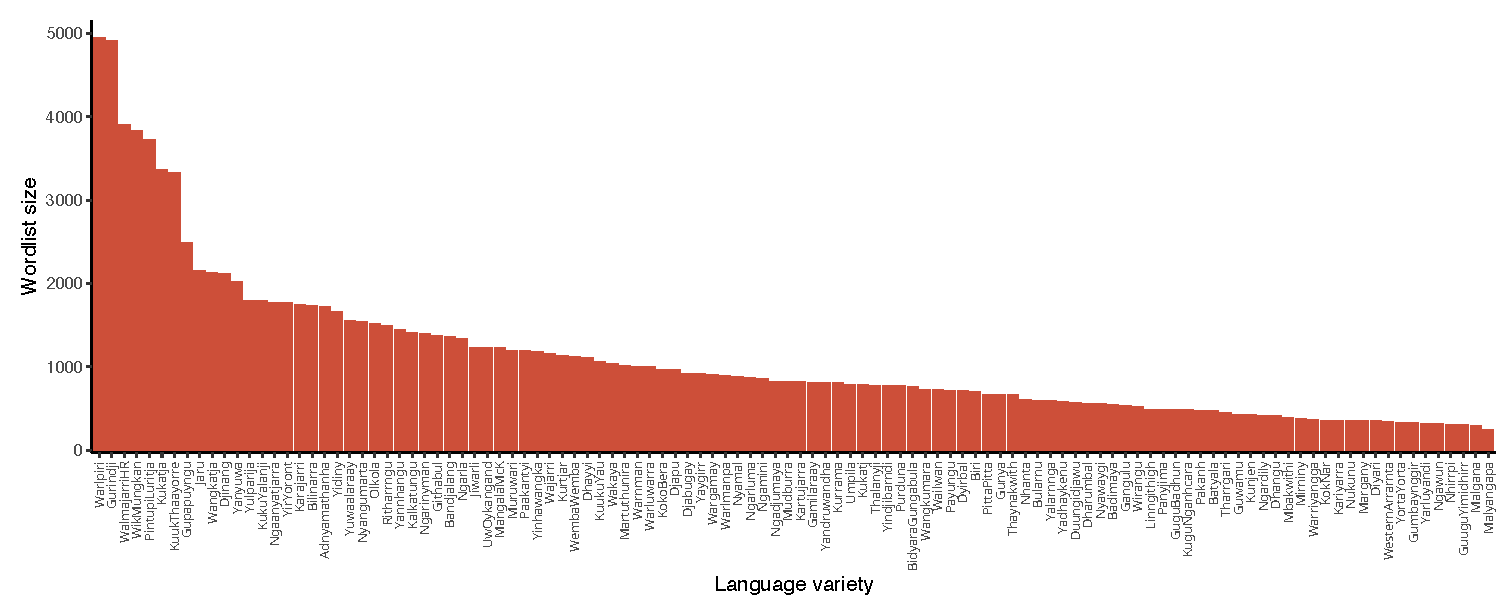
\includegraphics[width=1\linewidth]{05-phylo-signal/fig/wordlist_sizes} 

}

\caption[Lexicon sizes]{Lexicon sizes.}\label{fig:lex-size}
\end{figure}

Original source data, which is typically orthographic and, if digital, is sometimes mixed with metadata or other extraneous material, has undergone extensive data scrubbing, conversion to phonemic form using language-specific orthography profiles \autocite{moran_unicode_2018}, and additional automated and manual error checking. These procedures ensure basic data cleanliness. Separately however, it has long been recognised that the segmental-phonological analysis of languages is a non-deterministic process \autocites{chao_non-uniqueness_1934}{hockett_problem_1963}{hyman_universals_2008}{dresher_contrastive_2009}. Two linguists faced with the same data may produce different analyses, not due to error but due to different applications of the very many analytic criteria that figure into any analysis of segments. Consequently, the cross-linguistic phonological record varies not only according to language facts per se, but due also to variation in the practice of linguistic analysis. Recent literature \autocites{lass_vowel_1984}{hyman_universals_2008}{van_der_hulst_phonological_2017}{round_matthew_2017}{kiparsky_formal_2018} emphasises the value of normalising source descriptions prior to the analysis of cross-linguistic phonological datasets. This is not an information destroying process---it does not `standardise' languages---but it may shift information from one part of the representation (e.g., contrast between individual symbols) to another (e.g., contrasts between sequences of symbols), in order that information is located in a comparable way across the languages in the dataset, and therefore is more amenable to comparative analysis. Our wordlist data is normalised is this sense. Complex segments are split into simple sequences (e.g., prenasalised stops are split into a homorganic nasal + stop sequence); long vowels are represented as a sequence of identical short vowels, and vowel-glide-vowel sequences in which the glide is homorganic with either vowel are normalised to vowel-vowel; fortis consonants are represented as a sequence of identical short consonants, and positionally neutralised fortis/lenis stops as singletons; laminal consonants which do not figure in a pre-palatal versus dental opposition are represented as palatal, and rhotic glides which do not figure in an alveolar versus post-alveolar opposition are represented as post-alveolar \autocites[see also][]{round_phonemic_2019}{round_australian_2019}. The phonotactic character sets used in this study were extracted from these normalised, comparably segmented wordlists.

\hypertarget{ref-phylogeny}{%
\subsection{Reference phylogeny}\label{ref-phylogeny}}

The reference phylogeny we use is a maximum clade credibility tree\footnote{Bayesian phylogenetic methods return not a single phylogenetic tree but a posterior distribution of many possible trees. These trees can be summarised into a single maximum clade credibility tree with confidence levels for each node in the tree, corresponding to how frequently that node appears in the posterior sample. It is the maximum clade credibility tree that we use for a reference phylogeny in this study. See \textcite{bowern_computational_2012} and \textcite{bouckaert_origin_2018} for a full explanation of the methods used to infer the phylogenies considered in this section.} of 285 Pama-Nyungan language varieties inferred using lexical cognate characters by the second author (Figure S1, Supplementary Information). It was inferred independently of this study, prior to this study's conception and without the involvement of the first and third authors. It was inferred using the same Stochastic Dollo model as \textcite{bowern_computational_2012}, but with an expanded and refined dataset. Further details of the model and phylogeny construction are described in \textcite{bowern_computational_2012}, \textcite{bowern_pama-nyungan_2015} and \textcite{bouckaert_origin_2018}. The cognate dataset used to infer the reference phylogeny is available on Zenodo \autocite{bowern_pama-nyungan_2018}. See Section S1 of the Supplementary Information for more information on the reference phylogeny.

We considered a reference tree from a newer phylogeographic analysis of Pama-Nyungan based on largely the same data plus further expansion to 304 doculects and continued refinement \autocite{bouckaert_origin_2018}, however, we opted against its use for this particular study. The reason for this is that, although Bayesian inference of phylogenetic tree topology is considered generally robust to the levels of lexical borrowing observed among Pama-Nyungan languages \autocites{greenhill_does_2009}{bowern_does_2011}, borrowing still has the effect of reducing branch lengths across the tree \autocite{greenhill_does_2009}. This effect, and consequently the accuracy of branch length estimates, is equally applicable to both trees considered here. However, the geographic element in the phylogeographic study uses, in part, branch lengths to model geographic dispersal. The posterior distribution of trees, which is jointly informed by cognate data and geography, may therefore show a bias towards geographically proximal languages whose apparent divergence times have been reduced by high rates of borrowing. Thus, although branch length estimates will be impacted by borrowing in any phylogenetic study of Pama-Nyungan, there is more chance of borrowing affecting topology in the phylogeographic study.

We consider it unlikely that the overall conclusions of the study would be altered by the choice of which version of the Pama-Nyungan phylogeny we use as a reference tree. Each of the studies referenced above produced highly congruent Pama-Nyungan phylogenies \autocite[for a detailed comparison, see][]{bouckaert_origin_2018}. Furthermore, \textcite{bouckaert_origin_2018} features fixed clade priors based on subgroups identified in earlier studies, so topological differences are constrained to some extent by design. Nevertheless, the accuracy of the reference tree is a key assumption of the methods we use in this study, and thus phylogenetic uncertainty is an important consideration. We return to this point in Section \ref{overall-robustness} and evaluate the overall robustness of our results to phylogenetic uncertainty by replicating a subset of phylogenetic signal tests over a posterior sample of trees.

As discussed above, we treat each wordlist in our study as its own doculect. The reference tree in this study was inferred using a similar approach, while remaining less-committal about the particular status of the unit of analysis. Resources were sometimes combined for a particular language, but they are also frequently broken up into separate units, particularly when the resources come from different authors and different time periods. We have taken care to match the wordlists in this study to their exact or best corresponding tip in the reference tree. In most cases, the wordlists we use here are the same as those used to generate the cognacy judgements used to infer the reference phylogeny. In other cases, we use a different source to the one used for the reference phylogeny but there is, nevertheless, a straightforward one-to-one mapping between the language variety our wordlist represents and a corresponding tip in the tree. In one case, our Mudburra source \autocite{nash_mudburra_1988} matches neither of the sources for the two Mudburra tips in the reference phylogeny. However, the two varieties in the reference phylogeny have the same date. This entails that when either of them is removed from the tree, the exact same result is obtained in terms of tree geometry, which is what is significant for our investigation. Accordingly, we remove one and match our source to the other.

\hypertarget{phy-sig-bin}{%
\section{Phylogenetic signal in binary phonotactic data}\label{phy-sig-bin}}

In the simplest case, the phonotactics of different languages may be compared in terms of which sequences of two segments (\emph{biphones}) they permit and which they do not. If claims about the relative homogeneity of phonotactic constraints in Australian languages holds, then we would expect this kind of comparison to yield little, if any, phylogenetic signal.

In this test, we construct the dataset as follows: We automatically extract from all wordlists every unique sequence of two segments---or more accurately, sequences of \(xy\) where each of \(x\) and \(y\) is either a phonological segment or a word boundary `\#'. Each sequence becomes a character (variable) in the dataset, for which every language receives a binary value: 1 if the sequence \(xy\) is found in the language's wordlist (even if only once); 0 if the language contains both segments in its inventory but the sequence \(xy\) never appears in its wordlist; or, NA (not applicable, missing) if the language does not contain one (or both) of either segment \(x\) or \(y\) in its inventory (and therefore cannot contain the sequence \(xy\) a priori). Binary data of this kind represents sequence permissibility: Where a language contains both segments in its inventory, it will either permit them to appear together in sequence or it will not. In this respect, the information encoded by these characters is similar to what one might find in the phonotactics section of a descriptive grammar, where one often encounters a description in prose and/or a basic tabulation of which segments are permitted and where, within syllable and word structures. However, this kind of information is also, in a sense, quite coarse-grained, since there are only two possible values. A sequence which is very common in one language will be coded in exactly the same way as a sequence which only appears a handful of times in another language.

We apply the \(D\) test individually to each character in the dataset that meets two conditions: at least 50 non-missing values (due to the aforementioned reliability issue with sample sizes smaller than this) and at least one instance of variation (we do not test characters where all languages share identical 1 or 0 values). Given the extensive history of description of Australian languages as phonotactically homogeneous, our prior expectation is that testing binary data will fail to yield significant phylogenetic signal. Indeed, we might expect that \(D\) will fall significantly below 0, indicating that values are clumped among tips on the reference phylogeny even more conservatively than would be expected if they had evolved in the same phylogenetic pattern as lexical data.

To evaluate the statistical significance of \(D\) for any given character, a \(p\) value is estimated for each of two null hypotheses: The null hypothesis that \(D = 1\) (\(H_{0(D=1)}\), character values are distributed randomly with regards to phylogeny) and the null hypothesis that \(D = 0\) (\(H_{0(D=0)}\), character values are distributed as could be expected if the character has evolved along the phylogeny according to a Brownian motion model). Each \(p\) value is calculated using the permutation procedure described at the end of Section \ref{phylo-sig-overview}. Our distributions of randomly simulated and phylogenetically simulated sums of sister tip/clade differences (\(\Sigma d_r\) and \(\Sigma d_b\)) are obtained via 10,000 permutations per biphone. The conventional cutoff for statistical significance is \(p = 0.05\). Here, we use the corresponding Bonferroni-corrected cutoff of 0.025.\footnote{Bonferroni correction is used because the conventional threshold for statistical significance, 0.05, represents the expected chance of a false discovery (false positive). This figure is known as the type I error rate (\(\alpha\)). The chance of a false discovery is multiplied when multiple tests are carried out. Bonferroni correction, which involves dividing the threshold for statistical significance by the number of tests being conducted, ensures that the chance of observing a false positive in any of the set of tests remains at the conventional rate, \(\alpha = 0.05\). In our case, two null hypotheses are tested for each character, hence we divide the threshold for statistical significance by two, ensuring the chance of a false positive for any particular character is 0.05.} For any given character, there are six possible results:

\begin{itemize}
\tightlist
\item
  \(D\) is significantly below 0. Character values are even more tightly clumped among close relatives than Brownian motion alone would lead us to expect.
\item
  \(D\) is significantly below 1 and not significantly different from 0. The data patterns phylogenetically, i.e., there is phylogenetic signal.
\item
  \(D\) is significantly above 0 and below 1. The data is neither clearly random nor clearly phylogenetic.
\item
  \(D\) is significantly above 0 and not significantly different from 1. It is consistent with randomness, not phylogeny.
\item
  \(D\) is significantly above 1. It is even more dispersed than expected via a random process.
\item
  \(D\) is not significantly distinct from 0 nor 1. The patterning of the data is indeterminate, and cannot be distinguished from randomness nor from Brownian phylogenetic evolution.\footnote{Technically, an indeterminate result can also arise in the seemingly contradictory instance that \(D\) is significantly below 0 but not significantly distinct from 1. This can happen when the distributions of phylogenetic and random simulations are highly overlapping and the random distribution is wider and flatter than the phylogenetic distribution. We observed one instance of this for a biphone with a single `1' value and 72 `0' values. As one would expect when every language but one shares the same value, this biphone is more clumped than in almost all simulations---99.25\% of phylogenetic simulations and 98.57\% of random simulations. This makes the biphone statistically significantly more clumped than the phylogenetic expectation but fractionally misses the threshold for statistical significance (98.75\% for a Bonferroni-corrected, two-tailed \(p\) test) in determining whether it is significantly different from the random expectation. This rare anomaly can only occur in cases of extremely skewed data (for example, when all languages share an identical value except for one outlier language), where phylogenetic and random simulations tend to overlap. We discuss the effect of highly skewed data and the effect of removing such data in Section \ref{phy-sig-bin-robustness} below.}
\end{itemize}

To summarise, the testing procedure proceeds as follows. For each binary biphone character, if the character has at least 50 non-NA values \emph{and} the character has at least one `1' and one `0' value (i.e., not every value is identical), then test as follows (otherwise discard):

\begin{itemize}
\tightlist
\item
  Calculate \(D\).
\item
  Conduct randomisation procedure to calculate \(p\) for \(H_{0(D=0)}\).
\item
  Conduct randomisation procedure to calculate \(p\) for \(H_{0(D=1)}\).
\end{itemize}

A result is interpreted from the combination of \(D\) and two \(p\) values.

\hypertarget{phy-sig-bin-results}{%
\subsection{Results for binary phonotactic data}\label{phy-sig-bin-results}}

We estimate \(D\) for 415 biphone characters using a script based on the \emph{phylo.d} function in the \emph{caper} package \autocite{orme_caper:_2013}, implemented in the statistical software \emph{R} \autocite{r_core_team_r:_2017}\footnote{The dataset for this and subsequent tests are available on Zenodo at \url{http://doi.org/10.5281/zenodo.3988775}. This repository also includes a full table of results and the R scripts used to perform the analysis and produce figures for the paper. See Section S3 of the Supplementary Information for usage instructions and a full description of these materials.}. The 415 \(D\) values cluster centrally around a mean of 0.43. The distribution is leptokurtic (kurtosis = 11.42), meaning there are more outliers relative to a normal distribution, making the distribution appear as a tall, narrow peak with long tails (Figure \ref{fig:d-density}). The standard deviation is large (3.74).

\begin{figure}[tbp]

{\centering 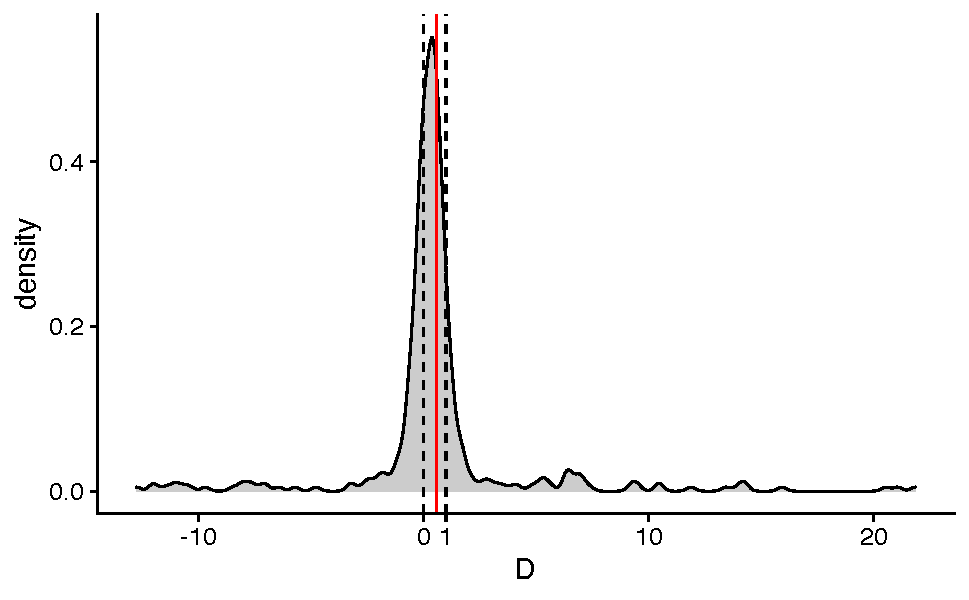
\includegraphics[width=0.66\linewidth]{05-phylo-signal/fig/d-density} 

}

\caption[Density of $D$ estimates for binary biphone characters]{Density of $D$ estimates for binary biphone characters. Dotted lines mark $D=0$, the phylogenetic expectation, and $D=1$, the random expectation. Mean $D$ for all characters is 0.43, marked in red.}\label{fig:d-density}
\end{figure}

The \(D\) test was of indeterminate significance for half of all characters (234 characters, 56\% of the dataset). The \(D\) scores for 160 characters (39\% of the total dataset) show evidence of phylogenetic signal. Just 17 characters (4\%) show the opposite result, where the character is consistent with randomness and there is no phylogenetic signal present. Both null hypotheses are rejected for the remaining 4 characters, all of which are more clumped than their phylogenetic expectation. None fall somewhere between phylogenetic and random expectations (where \(D\) is significantly above 0 but significantly below 1), nor are any significantly more dispersed than the random expectation. The distribution of these results among different biphone characters is plotted in Figure \ref{fig:d-swatch}. Note that we expect around 5\% of null hypothesis rejections (approximately 9 of 185 rejected null hypotheses) to be false discoveries. Nevertheless, when considering the whole dataset as an ensemble rather than each character individually, a general result can be discerned. The clearest conclusion is that binary, permissibility-based characters tend to be low yielding in information, giving a statistically significant outcome in fewer than half of cases. Nevertheless, where a significant result can be determined, phylogenetic signal does tend to be present---to a degree that is perhaps surprising in light of previous literature describing the relative homogeneity of Australian phonotactic restrictions and their lack of utility in historical endeavours. This result suggests there may be a greater degree of historical information contained in Pama-Nyungan phonotactics than previously thought. However, it may be that a finer-grained approach to data extraction is needed in order to detect it.

These results can be compared to two earlier studies performing the same test on much smaller samples of languages. In the first, \textcite{macklin-cordes_high-definition_2015} find no evidence for phylogenetic signal in the Yolngu subgroup of Pama-Nyungan---rather, data are significantly over-clumped, suggesting a higher degree of conservatism in phonotactic restrictions relative to lexical data. They fail to reject a null hypothesis of \(D = 0\) for Ngumpin-Yapa, suggesting there may be a degree of phylogenetic signal in the Ngumpin-Yapa dataset. However, the pilot study results should be treated with caution---particularly the failure to reject the \(D = 0\) null hypothesis in the case of Ngumpin-Yapa---due to the small sample sizes (10 languages for Ngumpin-Yapa, 7 for Yolngu), well below the minimum of 50 taxa recommended by \textcite{fritz_selectivity_2010}. \textcite{dockum_phylogeny_2018} performs the same analysis using biphone characters from 20 Tai language varieties of the Kra-Dai family. In contrast to \textcite{macklin-cordes_high-definition_2015}, Dockum finds some evidence of phylogenetic signal in the Tai data and suggests perhaps the earlier result was due to insufficient variation in that particular language sample rather than a limitation of binary biphone characters per se. Although the low information yield from binary data is to be expected, our results here appear to support Dockum's conclusion.

\begin{figure}[tbp]

{\centering 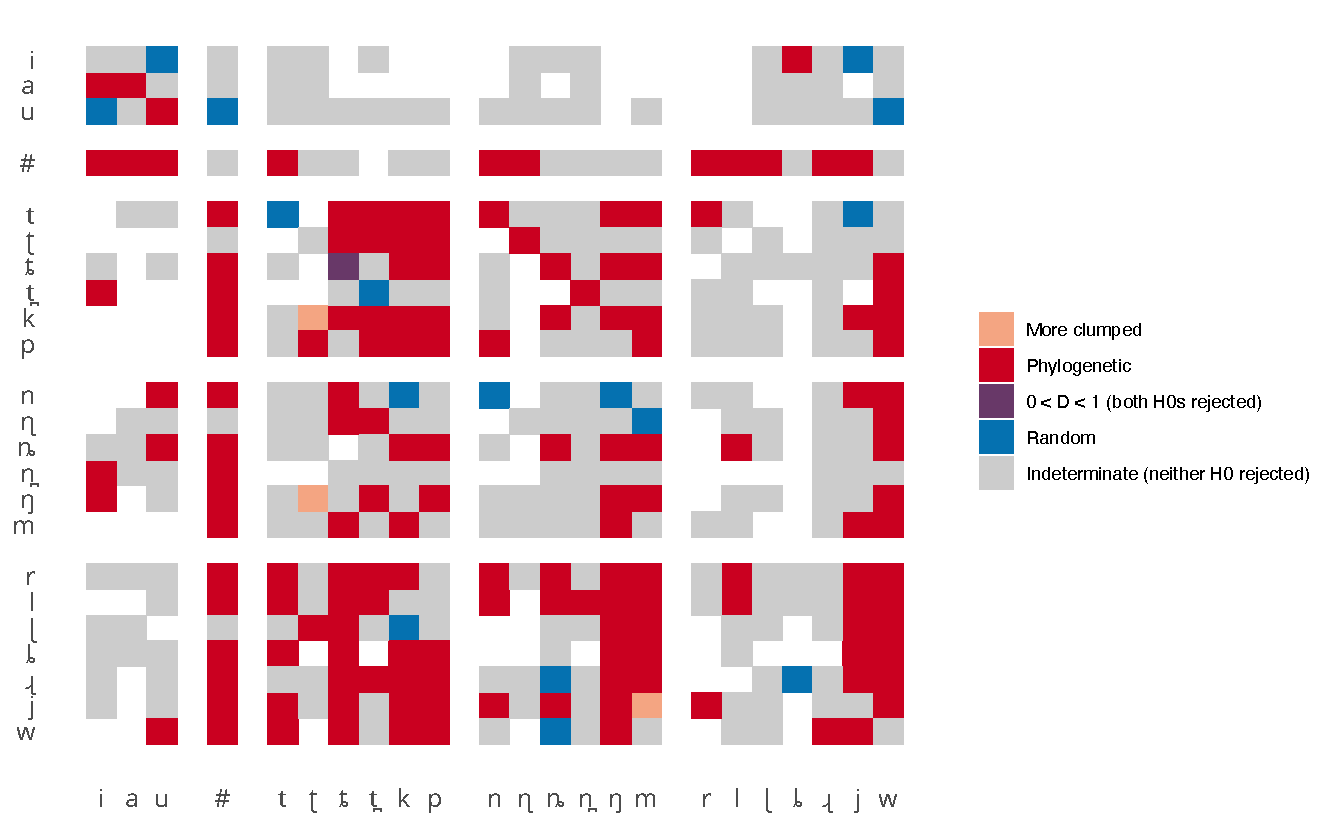
\includegraphics[width=0.9\linewidth]{05-phylo-signal/fig/d-sig-swatch} 

}

\caption[Phylogenetic signal significance testing for binary biphone characters]{Phylogenetic signal significance testing for binary biphone characters. This grid colour-codes each biphone character according to the results of its respective significance tests. The grid is arranged such that the vertical axis represents the first segment of the biphone and the horizontal axis represents the second segment. Besides a tendency for phonotactic restrictions at word boundaries to show phylogenetic signal, few patterns stand out. %Note that throughout, we use the symbols /ȶ, ȵ, ȴ/ to represent the alveo-palatals, as distinct from the dorso-palatals /c, ɲ, ʎ/.
}
\label{fig:d-swatch}
\end{figure}

\hypertarget{phy-sig-bin-robustness}{%
\subsection{Robustness checks}\label{phy-sig-bin-robustness}}

Given a sufficient number of taxa for which data are available (\textgreater{}50), \(D\) scores should reflect a degree of phylogenetic signal present in the data, independently of tree size (the number of taxa) and shape (branching patterns). To check this, in Figure \ref{fig:d-scatterplots}(A) for each character we plot its \(D\) score against the number of doculects for which it had non-missing values. Irrespective of the number of doculects that supply non-missing values, the \(D\) scores appear to cluster centrally around mean \(D\) for the dataset, suggesting that \(D\) is not being unduly affected by missing values for particular characters. A second check leads to rather different results, however. We check whether skewed distributions of character values affects \(D\) scores (Figure \ref{fig:d-scatterplots}(B)). Here, we consider the distribution of 1s and 0s for each character and plot \(D\) against how skewed the distribution of character values is towards a particular value. For example, a character where there are 108 `1' values in the dataset and only 4 `0' values will have a skewing rating of 0.96 (the count of `1' values, 107, divided by 112 total observations). Here, we find that when the ratio of 1s and 0s for a character is highly unequal, estimates of \(D\) tend towards extreme magnitudes while also being unrevealing, that is, statistically indistinguishable from 0 and 1.\footnote{Note that it is a desirable feature of the \(D\) test that it should return a lack of significance when there is a near-complete lack of variability in the data for the test to evaluate. This is an issue with the data, not the test.} As described above, Australian languages are known for homogeneity in phonological inventories and phonotactic restrictions, so consequently there are many characters with skewed distributions affecting the results. In Figures \ref{fig:d-density-filtered}--\ref{fig:d-swatch-filtered}, we plot a subset of the \(D\) test results, restricted to characters with less skewing.

\begin{figure}[tbp]
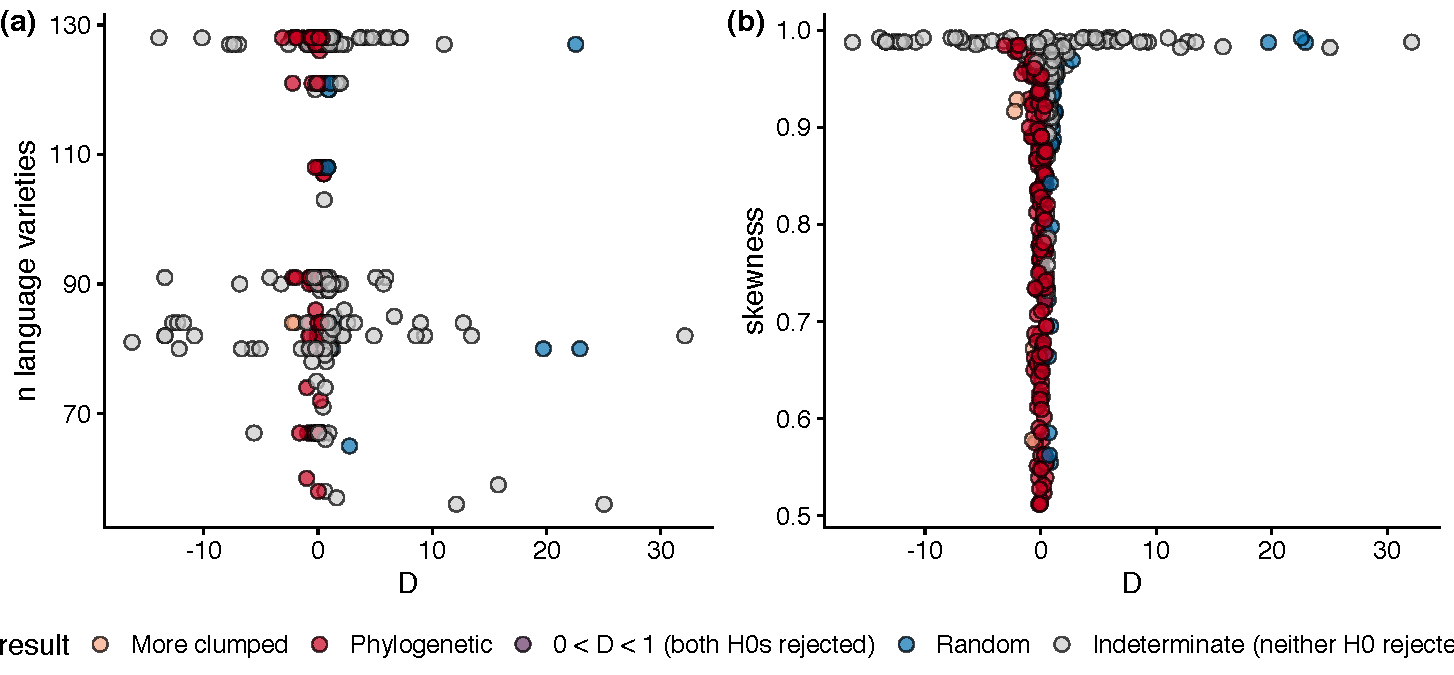
\includegraphics[width=1\linewidth]{05-phylo-signal/fig/d-scatterplots} \caption[Scatterplots of $D$ scores]{Scatterplot of $D$ scores against (A) the number of doculects with non-missing values for each character and (B) the skewing of the distribution of 1s and 0s for each character. $D$ clusters evenly around the mean regardless of the number of missing values. Variation in $D$ increases greatly among characters where all but 1 or a few doculects share the same value, but the results are overwhelmingly not significant.}\label{fig:d-scatterplots}
\end{figure}

\begin{figure}[tbp]

{\centering 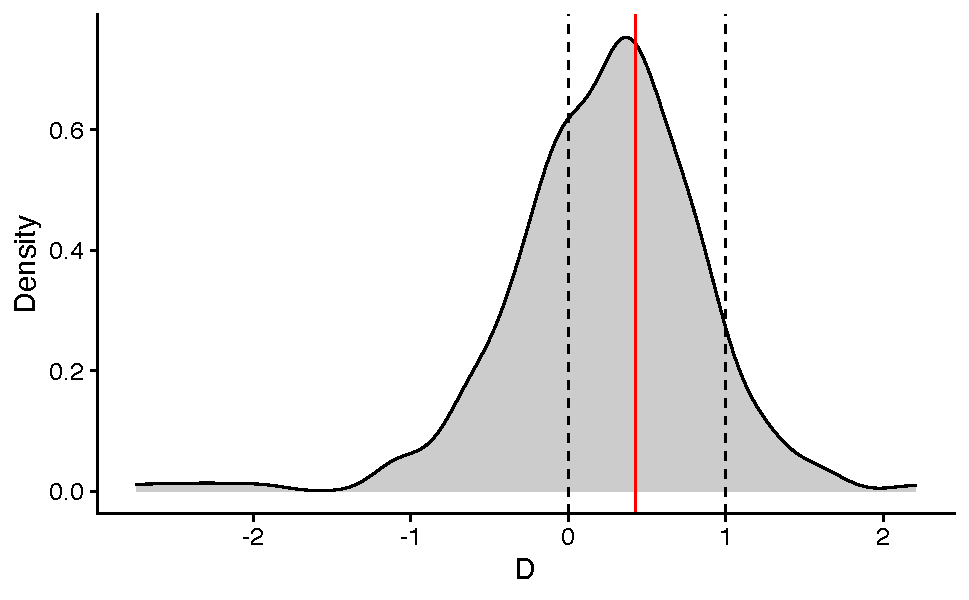
\includegraphics[width=0.66\linewidth]{05-phylo-signal/fig/d-density-filtered} 

}

\caption[Density of $D$ estimates for binary biphone characters, highly skewed characters removed]{Density of $D$ estimates for binary biphone characters where character values are skewed less than 97:3.}\label{fig:d-density-filtered}
\end{figure}

\begin{figure}[tbp]

{\centering 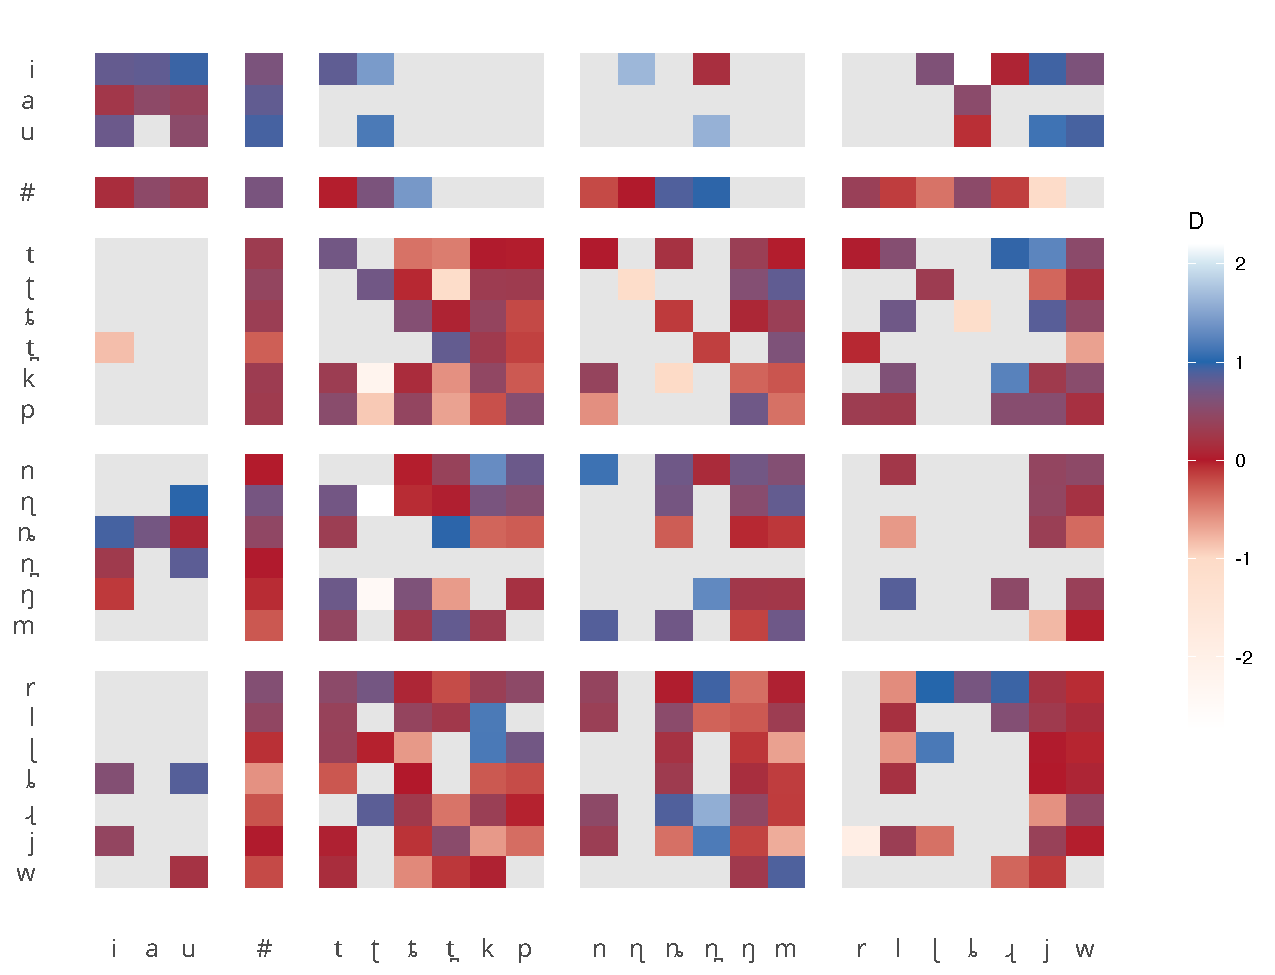
\includegraphics[width=0.75\linewidth]{05-phylo-signal/fig/d-swatch-filtered} 

}

\caption[$D$ scores for binary biphone characters, highly skewed characters removed]{$D$ scores for binary biphone characters where character values are skewed less than 97:3. Red shades show a character's proximity to $D=0$---darker red indicates stronger phylogenetic signal. Blue shades show a character's proximity to $D=1$, where character values are distributed randomly. This heat grid shows the proximity of each individual character's $D$ value to $D=0$, its expectation if the character evolved along the phylogeny following a Brownian motion process. The vertical axis represents the first segment of the biphone, the horizontal axis represents the second segment.}\label{fig:d-swatch-filtered}
\end{figure}

\hypertarget{phy-sig-cont}{%
\section{Phylogenetic signal in continuous phonotactic data}\label{phy-sig-cont}}

We test whether a higher degree of phylogenetic signal is detectable in continuous-valued biphone characters. As in the previous test, we take every possible sequence of two segments, or biphones, in our sample of 112 Pama-Nyungan wordlists. In this case, however, rather than simply coding for the presence of a biphone in a language's lexicon, we consider the relative frequencies of transitions between the segments in that biphone across the language's lexicon. For each biphone character, we take two values: The Markov chain forward transition probability---that is, for a biphone \(xy\), the probability of \(x\) being followed by \(y\), normalised over all instances of \(x\). This captures, if only in a basic way, our awareness that words do not consist of strings of independent segments, but rather the probability of observing some segment is very much dependent on what came before it. Secondly, we take Markov chain backward transition probabilities---that is, for the biphone \(xy\), the probability of \(y\) being preceded by \(x\), normalised over all instances of \(y\) in the lexicon. The frequency characters we extract come from wordlists. This is advantageous in that they are somewhat independent of word frequency effects since each word is counted only once, in contrast to frequencies extracted from language corpora. On the other hand, speakers show sensitivity to phoneme frequencies in language use (for example, when coining novel words) \autocites{coleman_stochastic_1997}{zuraw_patterned_2000}{ernestus_predicting_2003}{albright_rules_2003}{eddington_spanish_2004}{hayes_stochastic_2006}{gordon_phonological_2016} so word frequency will likely have some effect on phoneme and biphone frequency even in a wordlist. Investigation of phylogenetic signal in frequency characters extracted from corpora versus wordlists may be a possibility for future study.

We quantify phylogenetic signal by estimating \(K\) \autocite{blomberg_testing_2003} individually for each character, using the \emph{multiPhylosignal} function, in the \emph{picante} package \autocite{kembel_picante:_2010}, in \emph{R} statistical software. The \(K\) test has somewhat greater statistical power than the \(D\) test, enabling us to apply the test to characters with as few as 20 non-missing values. Calculation of \(K\) works with non-zero values only, so zero values (where the language contains both segments \(x\) and \(y\) but \(x\) is never followed by \(y\), or vice versa) are considered not applicable and removed from calculation. A total of 490 characters (245 biphone forward transition probabilities and 245 backward transition probabilities) meet the criterion of at least 20 languages with non-missing and non-zero values for testing. Subsequently, to evaluate whether the level of phylogenetic signal is significant for a given character, we conduct Blomberg, Garland and Ives' (2003) randomisation procedure with 10,000 random permutations per character.

To summarise, this testing procedure proceeds as follows. For each biphone frequency character, if the character has at least 20 non-NA values \emph{and} the character has at least two unique frequency values (i.e., not every character value is the same), then test as follows (otherwise discard):

\begin{itemize}
\tightlist
\item
  Calculate \(K\).
\item
  Conduct randomisation procedure to calculate \(p\) for \(H_{0(K = 0)}\).
\end{itemize}

Mean \(K\) for all 490 characters is 0.54 (\(SD\) 0.21) (Figure \ref{fig:k-density}). This is comparable to certain physiological traits presented as examples of biological traits with a high degree of phylogenetic signal by \textcite{blomberg_testing_2003}, for example, \(K=0.55\) for log body mass of primates. Using the \textcite{blomberg_testing_2003} randomisation procedure, we find a statistically significant degree of phylogenetic signal for 351 of 490 characters (178 forward transition characters, 173 backward transition characters), or 72\% of the total dataset.

\begin{figure}[tbp]

{\centering 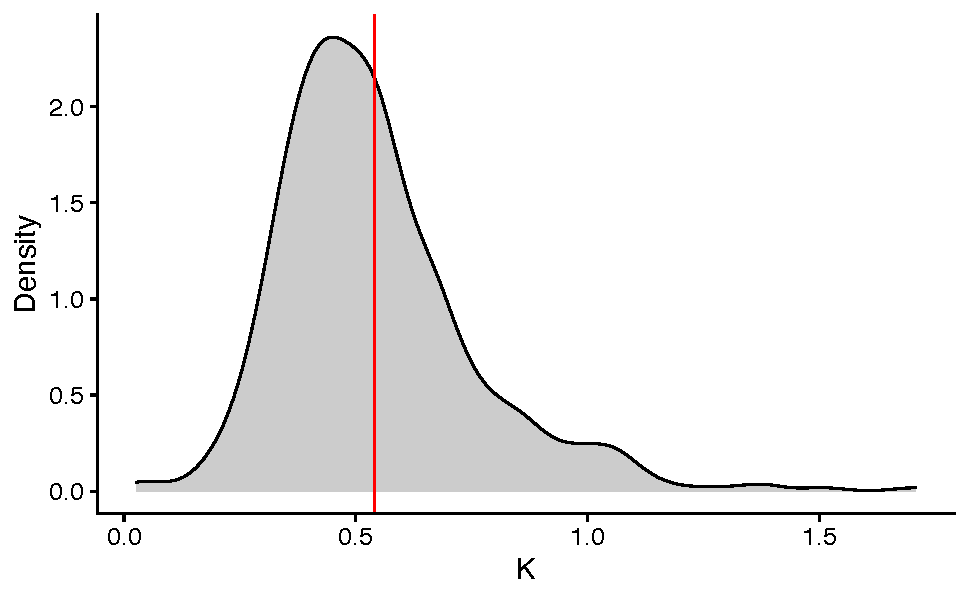
\includegraphics[width=0.66\linewidth]{05-phylo-signal/fig/k-density} 

}

\caption[Density of $K$ scores for all frequency-based biphone characters]{Density of $K$ scores for all frequency-based biphone characters (frequencies of both forward and backward transitions between segments).}\label{fig:k-density}
\end{figure}

We consider whether phylogenetic signal is higher or lower in certain kinds of biphone characters. Figure \ref{fig:k-swatch} shows a matrix of \(K\) scores for forward transition characters, with rows and columns arranged by phonological natural class. No clear pattern stands out.

\begin{figure}[tbp]

{\centering 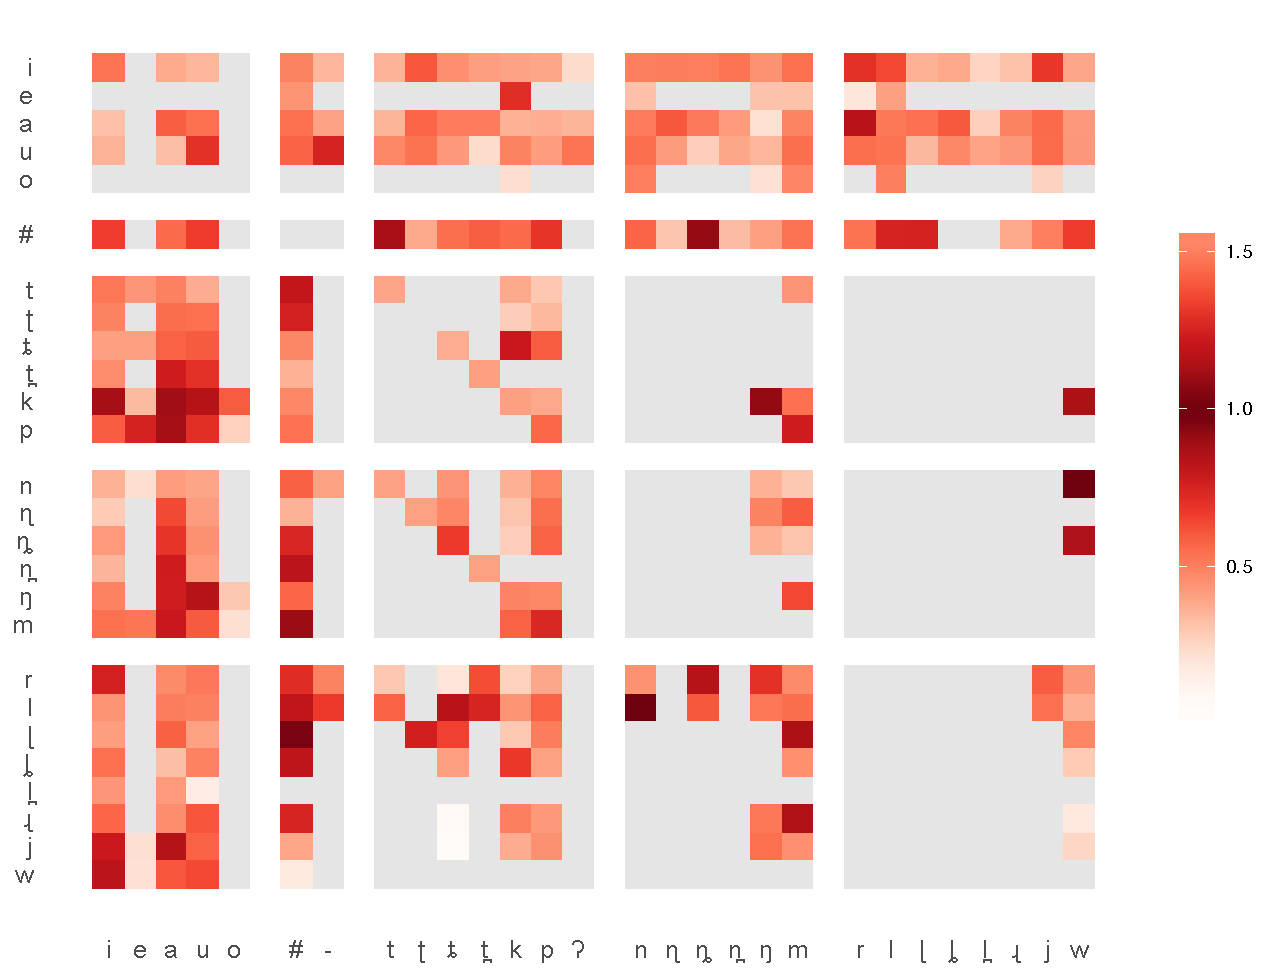
\includegraphics[width=0.75\linewidth]{05-phylo-signal/fig/k-swatch} 

}

\caption[Phylogenetic signal for forward transition frequencies]{Phylogenetic signal for forward transition frequencies. This heat grid shows $K$ scores for biphone characters (forward transition frequencies only). Each square represents a biphone (where the first segment is listed on the vertical axis and second segment on the horizontal axis). Data points are taken from the frequencies of each biphone, $xy$, over the total frequency of segment $x$ in each language, and then phylogenetic signal $K$ is measured for each biphone. Darker red shades indicate a stronger degree of phylogenetic signal. As with the $D$ test, no clear pattern of high versus low $K$ scores stands out, although there is a high degree of phylogenetic signal in the dataset overall.}\label{fig:k-swatch}
\end{figure}

\hypertarget{phy-sig-cont-robustness}{%
\subsection{Robustness checks}\label{phy-sig-cont-robustness}}

Although \(K\) is intended to be a measure of phylogenetic signal that is independent of tree size and shape, tree size and shape can have some effect on results in practice \autocite{munkemuller_how_2012}. We wish to check that the Pama-Nyungan tree does not contain any unusual properties that could cause either the K statistic or the randomisation procedure to perform unexpectedly. To do this, we allow simulated characters to evolve specifically along the Pama-Nyungan reference tree. We vary the model of evolution, between perfect Brownian motion along the entire tree and pure randomness generated directly at the tips of the tree, by mixing different strengths of Brownian phylogenetic signal and non-phylogenetic noise. 1000 traits are simulated at each percentage point interval for 100,000 total simulated traits (in other words, 1000 traits simulated with 100\% Brownian motion, then 1000 traits simulated with 99\% Brownian motion and 1\% randomness, and so on, until the traits evolve 100\% at random). Each simulated trait is then tested for statistical significance using the randomisation procedure described in Section \ref{phylo-sig-overview}, with 1000 repetitions to determine a \(p\) value. In a robust testing scenario, \(K\) will scale appropriately between 0 and 1 according to the level of Brownian motion and random noise being simulated, and the randomisation procedure will distinguish between traits with and without a significant degree of phylogenetic signal with a satisfactory amount of Type I (false positive) and Type II (false negative) errors.

The results are plotted in Figure \ref{fig:k-simulation-plots}. The \(K\) statistic shows a considerable degree of variability but, in the absence of substantial random noise, centres slightly below \(K=1\) which suggests the statistic is behaving as expected (if not slightly conservatively) when phylogenetic signal is present. For characters whose simulated evolution is near-random, the baseline of \(K\) seems to be elevated a little by our particular reference tree, with non-phylogenetic simulated characters ranging from the expected \(K=0\) to around \(K=0.3\). This should be kept in mind when interpreting \(K\) scores across our results. As for the randomisation procedure, Figure \ref{fig:k-simulation-plots}(B) shows the percentage of simulated traits that were identified as having a significant degree of phylogenetic signal (\(p < 0.05\)) at a given level of Brownian motion mixed with random noise. Above around 65\% Brownian motion, there are no Type II errors. The ability to detect significant phylogenetic signal drops as the level of random noise increases beyond 35\%, though overall the test's sensitivity seems acceptable. At the opposite extreme, where characters are simulated completely at random (and, therefore, there is no phylogenetic signal to detect) the randomisation procedure falsely detects phylogenetic signal 5.4\% of the time, very close to the expected false discovery rate of 5\% (given the conventional threshold for statistical significance of \(\alpha = 0.05\)). On the basis of these simulations, we are satisfied that randomisation procedure is sufficiently robust, given the particular size and shape of the Pama-Nyungan reference phylogeny.

\begin{figure}[tbp]

{\centering 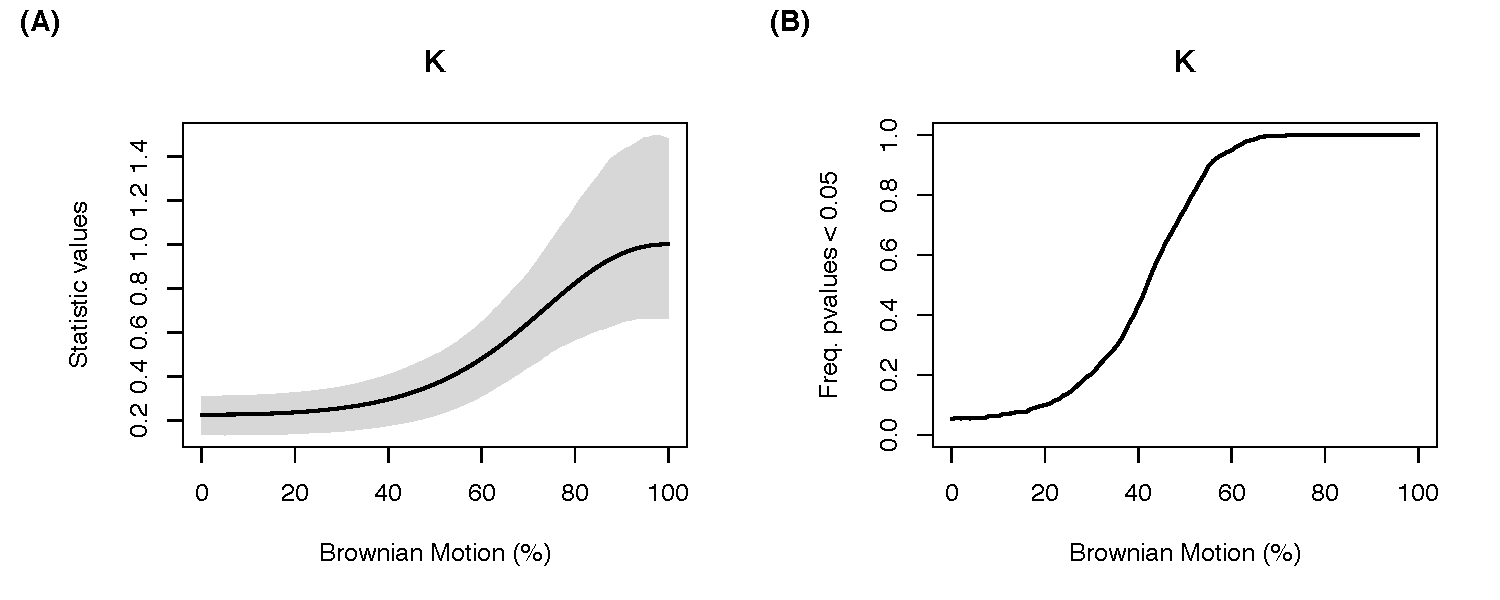
\includegraphics[width=0.9\linewidth]{05-phylo-signal/fig/phylosim} 

}

\caption[Behaviour of the $K$ statistic and randomisation procedure with the Pama-Nyungan reference phylogeny]{Behaviour of the $K$ statistic and randomisation procedure with the Pama-Nyungan reference phylogeny. Artificial characters are simulated evolving along the phylogeny with varying levels of non-Brownian noise. When a pure Brownian motion process operates, $K$ averages around 1 as expected. Where there is no Brownian process at all (and therefore no phylogenetic signal) $K$ is elevated to around 0.2---likely an artefact of this particular tree size and shape.}\label{fig:k-simulation-plots}
\end{figure}

As a final check, we consider whether the \(K\) statistic might be affected by the quantity of missing or `not applicable' values for a given character. We inspect this visually by plotting, for all biphone characters, the relation between a biphone's \(K\) score and the number of language varieties with non-missing data points on which \(K\) was calculated (Figure \ref{fig:k-scatterplot}). When \(K\) is calculated on fewer than around 40 non-missing values, the statistic shows a wider degree of variability. In addition, phylogenetic signal is deemed statistically significant for fewer characters in this range, suggesting that the quantity of missing values is affecting the statistical power of the test. However, all \(K\) scores cluster centrally around the mean regardless of the number of languages with non-missing values, suggesting that the mean \(K\) we observe for the dataset overall is not significantly affected by missing data.

\begin{figure}[tbp]

{\centering 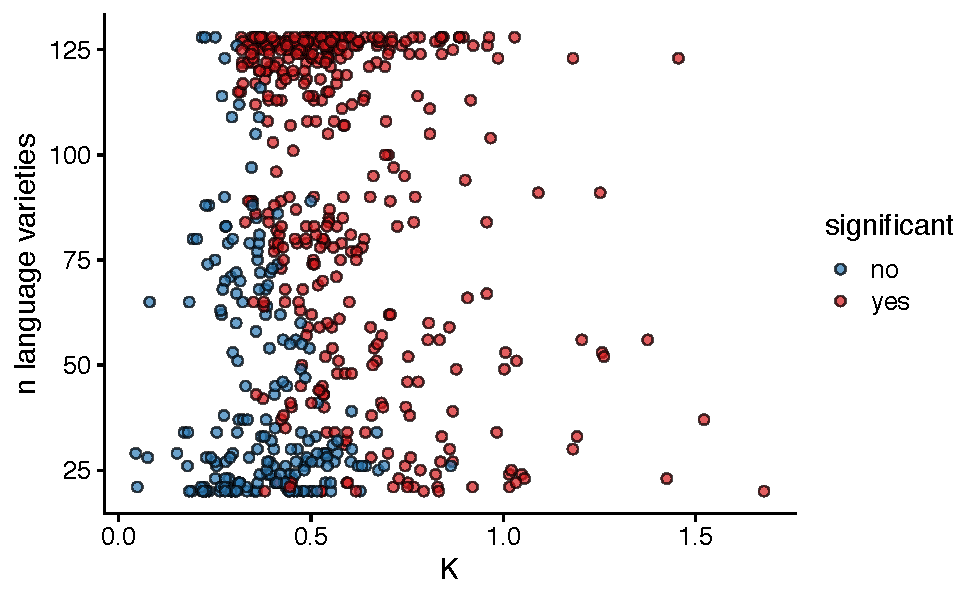
\includegraphics[width=0.66\linewidth]{05-phylo-signal/fig/k-scatterplot} 

}

\caption[Estimates of $K$ plotted against the number of doculects with non-missing values for each character]{Estimates of $K$ for forward and backward transition frequency characters plotted against the number of doculects with non-missing values for each character. Although some statistical power is lost and variability increases among characters with more missing values, $K$ scores cluster evenly around mean $K$ (0.52).}\label{fig:k-scatterplot}
\end{figure}

\hypertarget{fwd-vs-bkwd}{%
\subsection{Forward transitions versus backward transitions}\label{fwd-vs-bkwd}}

\begin{figure}[tbp]

{\centering 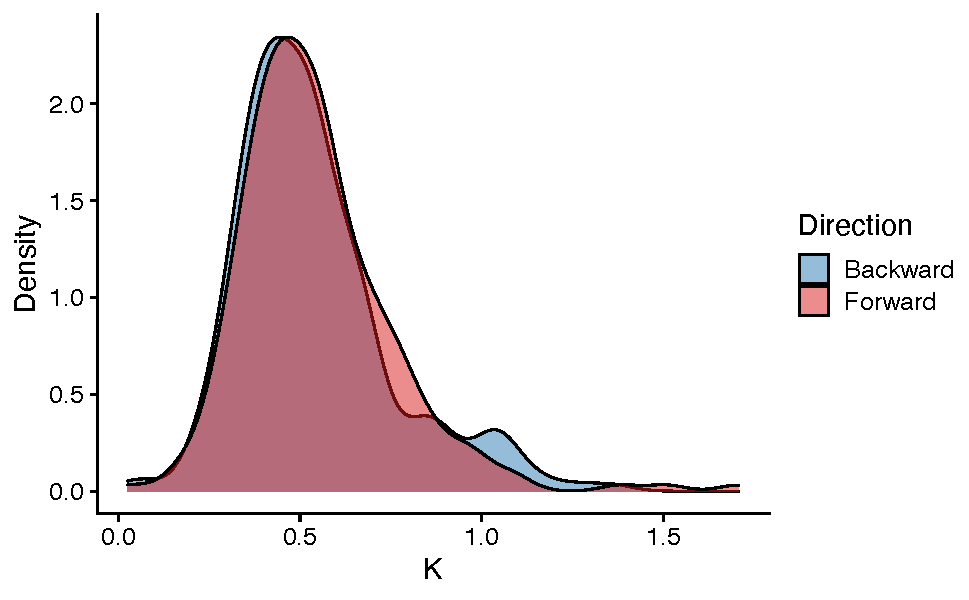
\includegraphics[width=0.66\linewidth]{05-phylo-signal/fig/k-fwd-bkwd} 

}

\caption[Distribution of $K$ scores for forward transition frequencies versus backward transition frequencies]{Distribution of $K$ scores for forward transition frequencies versus backward transition frequencies. We find no significant difference between these character types.}\label{fig:k-fwd-vs-bkwd}
\end{figure}

We find no significant difference in the means of \(K\) for forward transition characters (mean \(K =\) 0.544) and backward transition characters (mean \(K =\) 0.537) (\(t=\) 0.33, \(df=\) 487.97, \(p=\) 0.74, 95\% CI {[}-0.03, 0.04{]}). The distributions of \(K\) scores for forward and backward transitions are plotted in Figure \ref{fig:k-fwd-vs-bkwd}, showing a high degree of overlap between the two.

\hypertarget{norm-characters}{%
\subsection{normalisation of character values}\label{norm-characters}}

Visual inspection of the density plots for each character shows there is a tendency for character data to be negatively skewed (the weight of the distribution is left-of-centre), although this is not universally the case. To test whether the particular, heavy-tailed nature of the data has an effect on tests for phylogenetic signal, we apply Tukey's Ladder of Powers transformation to each character in the dataset and re-run both the \(K\) test and randomisation procedure. This is a power transformation, which makes the data fit a normal distribution as closely as possible. It does this by finding the power transformation value, \(\lambda\), that maximises the \(W\) statistic of the Shapiro-Wilk test for normality for each character individually. For our purposes, this transformation is effectively a change in the evolutionary model: A Brownian motion process is still assumed---a character value may wander up or down with equal probability---but, in this model, character values shift up or down along a transformed scale.

Mean \(K\) for normalised character data is 0.55 (\(SD\) 0.2). Of 490 characters, 405 or 83\% (206 forward transitions, 199 backward transitions) contain phylogenetic signal significantly above the random expectation. There is no statistically significant difference between mean \(K\) for untransformed data (0.54) versus mean \(K\) for normalised data (\(t=\) 0.49, \(df=\) 972.26, \(p=\) 0.622, 95\% CI {[}-0.02, 0.03{]})---see Figure \ref{fig:orig-vs-nrmlzd}.

\begin{figure}[tbp]

{\centering 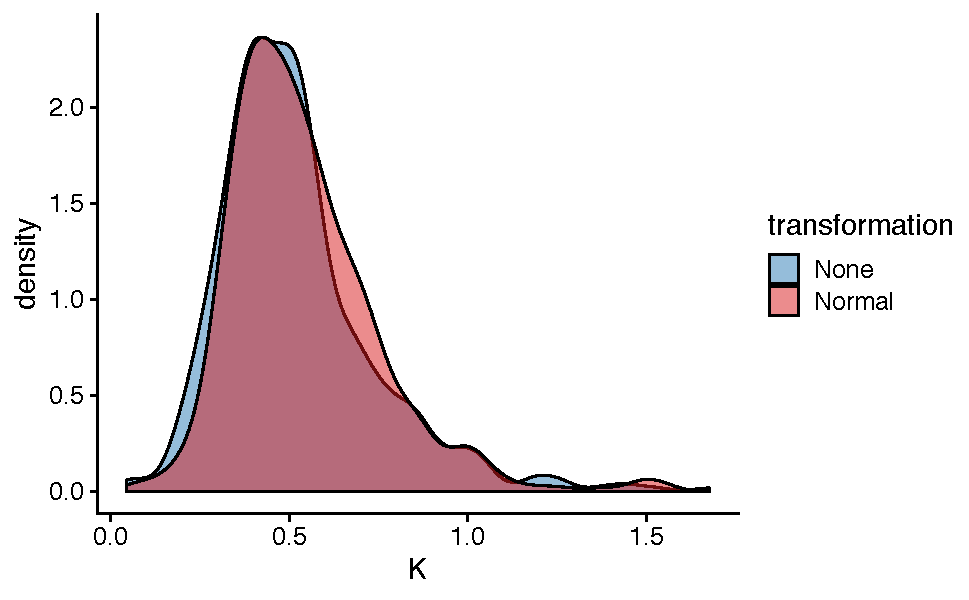
\includegraphics[width=0.66\linewidth]{05-phylo-signal/fig/k-orig-norm} 

}

\caption[Distributions of $K$ for untransformed character values and their normalised counterparts]{Distributions of $K$ for untransformed character values and their normalised counterparts. We find no significant difference between these distributions.}\label{fig:orig-vs-nrmlzd}
\end{figure}

\hypertarget{phy-sig-classes}{%
\section{Phylogenetic signal in natural-class-based characters}\label{phy-sig-classes}}

One limitation of analysing phylogenetic signal in biphone characters is the assumption that every biphone character is a statistically independent observation. In historical linguistic processes, however, phonological segments rarely behave independently. Rather, sound changes are applied to whole sound classes, thereby affecting any one of various cross-cutting sets of phonological segments (and, therefore, biphone characters we have used in this study).

To account for this non-independence and more faithfully model what we know about how phonotactic systems operate in a language, we extract forward and backward transition probabilities for sequences of phonological features. For the purposes of this experiment, word boundaries are counted as a class and vowels are reduced to a single `vowel' class. Three sets of characters are extracted: forward and backward transition probabilities between natural classes based on place of articulation (segments belonging to the following classes: word boundary, labial, dental, alveolar, retroflex, palatal, velar, glottal, vowel); forward and backward transition probabilities between natural classes based on major places of articulation, where coronal contrasts have been collapsed (word boundary, labial, apical, laminal, velar, vowel); and natural classes based on manner of articulation (word boundary, obstruent, nasal, vibrant, lateral, glide, rhotic glide, vowel). The choice of natural classes is based on well-established principles of organisation among segments in Australian languages \autocites{dixon_languages_1980}{hamilton_phonetic_1996}{baker_word_2014}{round_segment_2021}{round_phonotactics_2021}.

\begin{table}

\caption[Summary of $K$ analysis for forward and backward transition frequencies, comparing different natural classes]{\label{tab:k-natural-classes-summary}Summary of $K$ analysis for forward and backward transition frequencies between different natural classes. The two rightmost columns indicate the total number of characters analysed and the percentage of those characters with a significant degree of phylogenetic signal according to the randomisation procedure.}
\centering
\begin{tabular}[t]{lrrr}
\toprule
Classes & Mean K & n characters & significant (\%)\\
\midrule
Place & 0.61 & 126 & 94\\
Major place & 0.63 & 96 & 75\\
Manner & 0.59 & 88 & 66\\
\bottomrule
\end{tabular}
\end{table}

Table \ref{tab:k-natural-classes-summary} presents mean \(K\) and the proportion of significant characters for each of these three natural-class-based datasets. All show highly similar distributions (Figure \ref{fig:k-natural-classes}). There is no statistically significant difference in the means of \(K\) for the three feature types, according to a one-way ANOVA (\(F\)(2, 307) = 0.49, \(p=\) 0.616). An Anderson-Darling k-sample test, which tests the hypothesis that \(k\) independent samples come from a common, unspecified distribution (i.e., no prior assumption about normality) also finds no significant difference in the distributions of \(K\) scores for the three natural-class-based datasets (\(AD=\) 2.19, \(T.AD=\) 0.18, \(p=\) 0.329).

\begin{figure}[tbp]

{\centering 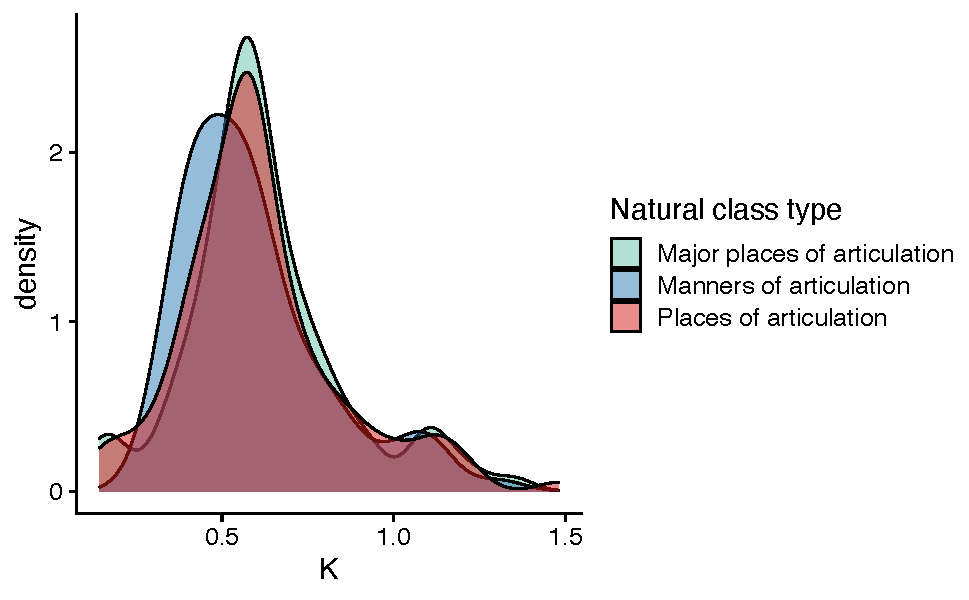
\includegraphics[width=0.66\linewidth]{05-phylo-signal/fig/k-natural-classes} 

}

\caption[Comparison of $K$ scores for transitions between different kinds of natural classes]{Comparison of $K$ scores for transitions between different kinds of natural classes. The differences between all three distributions are not statistically significant.}\label{fig:k-natural-classes}
\end{figure}

\hypertarget{classes-vs-biphones}{%
\subsection{Natural-class-based characters versus biphones}\label{classes-vs-biphones}}

\begin{figure}[tbp]

{\centering 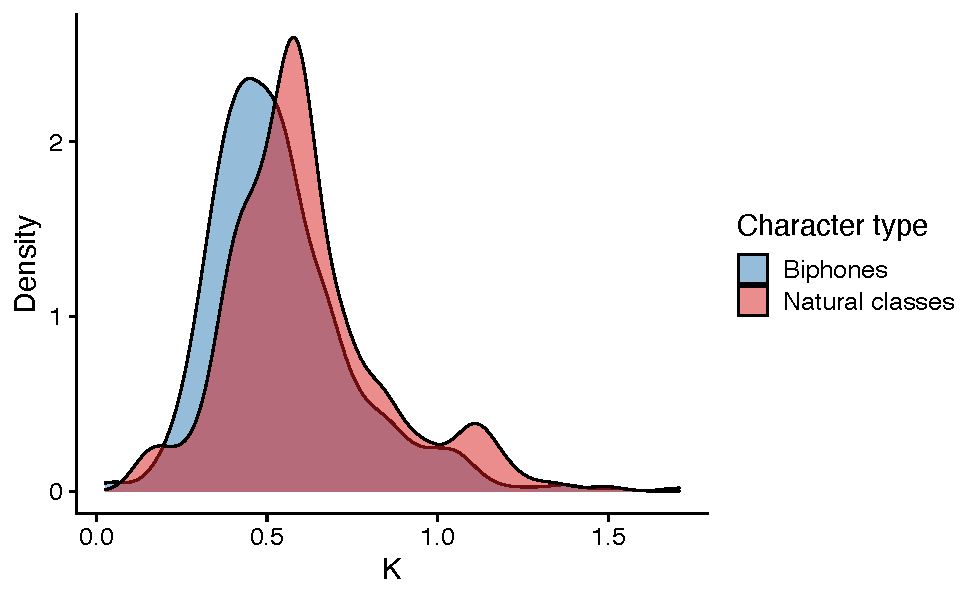
\includegraphics[width=0.66\linewidth]{05-phylo-signal/fig/k-biphones-classes} 

}

\caption[Distributions of $K$ scores for segmental biphone characters versus natural-class-based characters]{Distributions of $K$ scores for biphone characters, coding the relative frequencies of transitions between phonological segments, and natural-class-based characters, coding the relative frequencies of transitions between natural classes of segments. Phylogenetic signal is higher overall in the natural-class-based dataset than the biphone-based dataset}\label{fig:k-biphones-vs-features}
\end{figure}

We compare the degree of phylogenetic signal in the biphone data tested in Section \ref{phy-sig-cont} to the natural-class-based data tested here (see Figure \ref{fig:k-biphones-vs-features}). Mean \(K\) for all natural-class-based characters is 0.61, which is significantly higher than the mean \(K\) for biphone data, 0.54 (\(t=\) 4.38, \(df=\) 622.47, \(p < 0.001\), 95\% CI {[}0.04, 0.1{]}). The Kolmogorov-Smirnov test, which is more sensitive to the overall shape of the distribution than a t-test comparison of means, also finds a significant distinction between \(K\) for biphone characters and \(K\) for natural-class-based characters (\(D=\) 0.21, \(p < 0.001\)).

\hypertarget{phylo-sig-discussion}{%
\section{Discussion}\label{phylo-sig-discussion}}

Computational phylogenetic methods are increasingly commonplace in historical linguistics. However, there has been relatively less consideration of the range of data types that might profitably be used with computational phylogenetic methods, beyond traditional, manually-assembled sets of lexical cognate data. In this study, we have considered the potential utility of quantitative phonotactic data for historical linguistics, for the reasons that quantitative phonotactic data is (i) readily extractable from basic wordlists, and (ii) may show certain kinds of historical conservatism, where the historical signal in more traditional lexical data would be affected by borrowing and lexical innovation.

We extracted frequencies of transitions between phonological segments in scrubbed and comparably segmented wordlists representing 112 Pama-Nyungan language varieties. As points of comparison, we extracted two additional datasets: Firstly, a binarised version of the dataset, which simply records whether or not particular two-segment sequences, a.k.a. biphones, are present in a language's wordlist. This is to emulate, in a simple sense, the kind of information which is often recorded in the phonology section of published descriptive grammars. We also extracted frequencies for transitions between natural classes of sounds. This is to account (at least, to some partial degree) for the fact that phonological segments tend not to evolve independently but pattern into natural classes, thereby limiting the independence of biphone-based variables.

To test whether historical information is preserved in our phonotactic datasets, we tested for phylogenetic signal, that is, the degree to which variance in the data reflects the evolutionary history of the 112 language varieties. We took an independent phylogenetic tree, inferred by the second author using lexical cognate data, and assumed a simple Brownian motion model of evolution. Our first key finding is that a significant degree of phylogenetic signal is detected in all three datasets---binary, segment-based and sound-class-based. Finding phylogenetic signal in the binary dataset is somewhat surprising, given previous descriptions of homogeneity in the phonotactics of Australian languages. Our second key finding is that phylogenetic signal is significantly stronger in the higher-definition, frequency-based datasets than it is in binary dataset. In turn, phylogenetic signal in the sound-class-based dataset is significantly stronger than the segment-based datasets. We took a closer look at certain comparisons within datasets, namely, whether there is a difference between forward and backward transitions, different kinds of sound classes, or between original (heavy-tailed) data and transformed data (to more closely fit a normal distribution). In all three cases, no significant differences were found.

\hypertarget{overall-robustness}{%
\subsection{Overall robustness}\label{overall-robustness}}

One important assumption of our method is that the tree being used as a reference phylogeny is an accurate depiction of the phylogeny for the languages in question. It is impossible to verify if this assumption is being satisfied with complete certainty, since it is impossible to observe the past and record a phylogeny directly. Instead, we must rely on the best available data and methods to infer a best estimate of the true historical phylogeny. As described in Section \ref{ref-phylogeny}, the Pama-Nyungan phylogeny we use in this study was inferred by the second author using lexical cognate data and a Bayesian computational method that produces a large posterior sample of trees. The posterior sample contains a large number of trees, all of which have a relatively high plausibility, and relatively equal plausibility, of being correct. However, we require a single tree. We select it using the \emph{maximum clade credibility} method, which runs as follows. All trees contain hierarchies of clades. For any two trees, we can compare how many clades they share. In our posterior sample, we can ask which one tree shares the greatest number of clades with all others (we can also ask which trees rank second, third, fourth, etc. according to the same metric). Thus in Section 6 we used the maximum clade credibility tree drawn from our posterior sample of trees. This is a commonly used approach in the phylogenetic sciences for summarising many trees, using a single tree that is maximally representative of the whole sample. However, naturally there is no guarantee that the maximum clade credibility tree is the true tree. It may be the case that a better representation of the true Pama-Nyungan phylogeny (assuming it is best represented by a single tree) exists among the many other trees the posterior sample. This kind of uncertainty is known as phylogenetic uncertainty.

To evaluate the robustness of our results against phylogenetic uncertainty, we repeat the \(K\) test for phylogenetic signal using a set of alternative trees. Namely, we test a subset of sound-class-based characters against each of 100 trees that we select from the posterior sample. The subset of characters includes forward and backward transitions between place features, and forward and backward transitions between manner features. The trees selected are the 100 top-ranked trees in the posterior sample according to the maximum clade credibility metric. In this way, we incorporate a degree of uncertainty in the topology and branch lengths of the Pama-Nyungan phylogeny, while restricting our attention to a subset of the most representative alternatives in the posterior sample. Note that overall the Pama-Nyungan tree is quite well resolved, so these trees differ from one another only minimally.

\begin{figure}[tbp]

{\centering 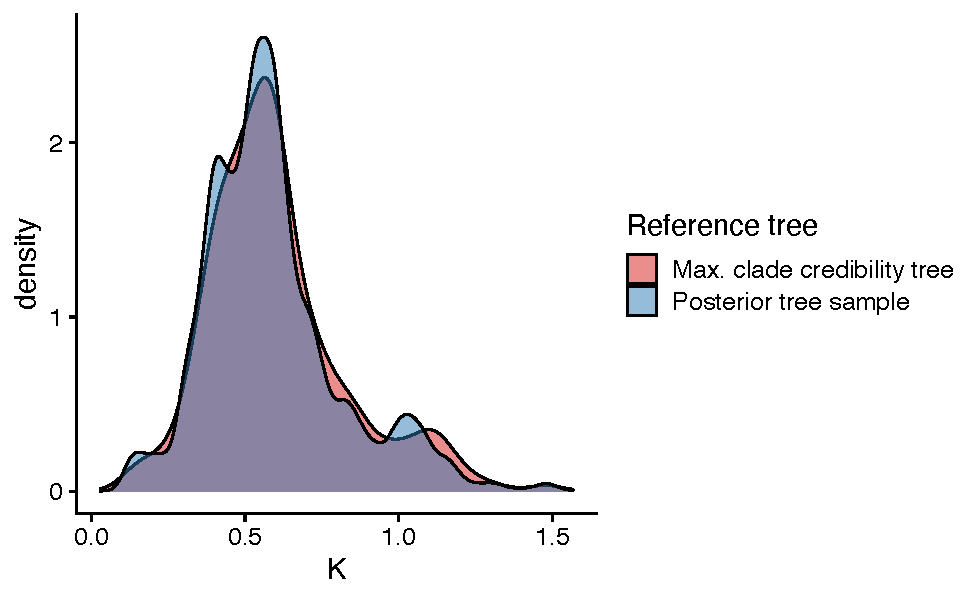
\includegraphics[width=0.66\linewidth]{05-phylo-signal/fig/k-mcct-posterior} 

}

\caption[$K$ statistics using a 100-tree posterior sample versus the maximum clade credibility tree alone]{Comparison of $K$ statistics using a 100-tree posterior sample versus the maximum clade credibility tree alone.}\label{fig:tree-uncertainty}
\end{figure}

214 sound class characters in total are tested, giving 21,400 \(K\) statistics in total (each character multiplied by 100 trees). The mean of these \(K\) scores is 0.59, which compares to a mean \(K\) of 0.6 for the same characters applied only to the maximum clade credibility tree as in Section \ref{phy-sig-classes}. This difference is not statistically significant (\(t=\) -0.92, \(df=\) 217.21, \(p=\) 0.359, 95\% CI {[}-0.05, 0.02{]}). The distributions of these \(K\) scores are illustrated in Figure \ref{fig:tree-uncertainty}. This result suggests our results are robust to phylogenetic uncertainty associated with our reference tree. The maximum clade credibility tree we use is not significantly inflating or deflating the \(K\) statistic.

A reviewer points out that we have only demonstrated robustness to phylogenetic uncertainty for a Pama-Nyungan phylogeny generated with a particular lexical dataset. We have not demonstrated robustness to potential further refinement of the Pama-Nyungan phylogeny that may come about with future expansion and/or refinement of the lexical dataset, and/or inclusion of data from other linguistic domains such as morphology. Future revisions of the Pama-Nyungan phylogeny will necessitate further robustness testing. The effect of such revisions may be to strengthen phylogenetic signal in phonotactic data (if limitations of the current phylogeny manifest as noise in the signal), weaken phylogenetic signal (if, for example, phonotactic data were to correlate more strongly with lexical data than morphological or other kinds of data), or be neutral in effect.

\begin{figure}[tbp]

{\centering 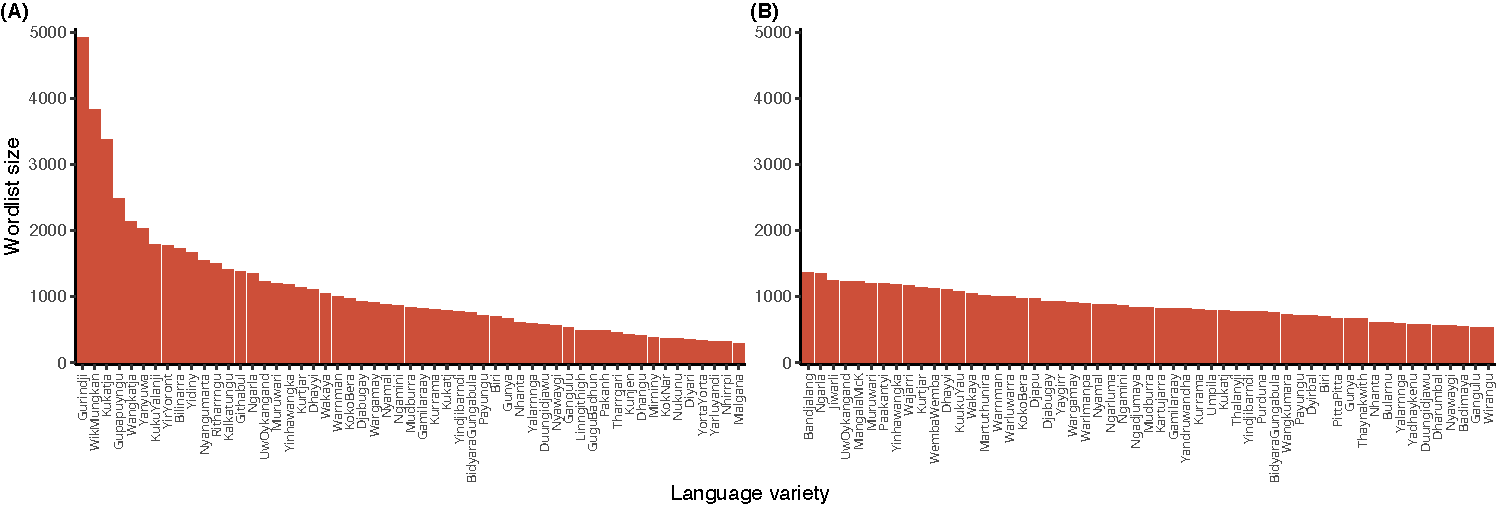
\includegraphics[width=1\linewidth]{05-phylo-signal/fig/wordlist_subset_sizes} 

}

\caption[Wordlists ranked by size]{Wordlists ranked by size. (A) shows every second wordlist in the language sample. (B) shows the middle 50\% of wordlists. Each subset contains the same number of wordlists but discrepancy in their size is greatly reduced in (B).}\label{fig:wordlist-subset-sizes}
\end{figure}

\begin{figure}[tbp]

{\centering 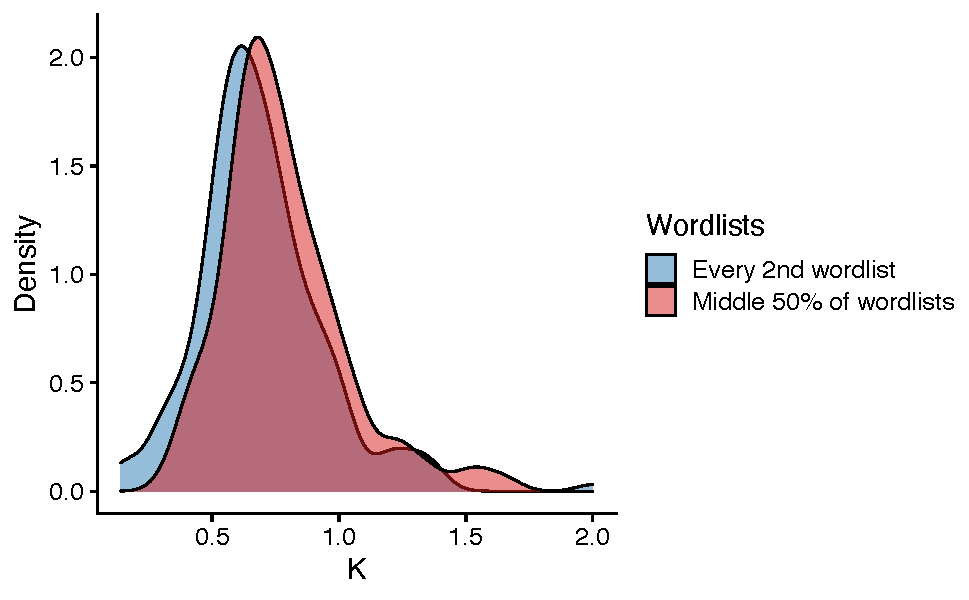
\includegraphics[width=0.66\linewidth]{05-phylo-signal/fig/k-IQR-vs-Every2nd} 

}

\caption[Comparison of $K$ statistics using middle quantile wordlists versus every second wordlist]{Comparison of $K$ statistics using only wordlists falling within the 25th and 75th quantiles (middle 50\%) for wordlist size, versus a sample of every 2nd wordlist (when ranked in order of size).}\label{fig:wordlist-uncertainty}
\end{figure}

In Section \ref{phylo-sig-wordlists} we mentioned that our wordlists vary significantly is size. The length of a wordlist can correlate with many other linguistic properties that it has. For instance, in our data, the number of entries in a wordlist and the mean phonemic length of those entries have a Pearson's correlation coefficient of \(r = 0.71\) (\(p < 0.001\)). That is, longer lists tend to contain longer words (presumably since shorter lists are weighted towards more basic, shorter vocabulary items). The existence of correlations like this means that it is not possible simply to `counterbalance' the length of wordlists by sub-sampling or resampling their items so that the resampled lists all have the same length. For example, the resampled lists that derive from longer underlying lists would still contain longer words. Nevertheless, it would still be desirable to know whether our results in Sections \ref{phy-sig-bin}--\ref{phy-sig-classes} are unduly influenced by the disparity in our wordlist lengths, by manipulating it in a controlled fashion. To do this, we extracted two different language sub-samples from our dataset. For the first, we ranked all wordlists by size and selected every second language, producing a sample half the original size but with the same disparity in lengths. For the second, we ranked all wordlists by size and selected the middle 50\% of the ranking, again producing a sample of half the size but this time with heavily reduced disparity, as shown in Figure \ref{fig:wordlist-subset-sizes}. Wordlists in the middle 50\% range in length from 528 to 1361 (mean 870).

For these samples, we ran \(K\) tests on the same subset of place and manner natural class characters as for the tree uncertainty robustness test above. Our reasoning is that if wordlist disparity strongly affects the estimation of phylogenetic signal, then we should see a clear difference in the results. Mean \(K\) for the middle 50\% of wordlists is 0.78, which is somewhat greater than the mean for every second wordlist, 0.69. This difference is small but statistically significant (\(t=\) 3.6, \(df=\) 425.76, \(p=\) 0, 95\% CI {[}0.04, 0.13{]}). This suggests that disparities in wordlist length are somewhat degrading the phylogenetic signal in our data, although there remains broad similarity between them, as pictured in Figure \ref{fig:wordlist-uncertainty}.

One attributing factor for this small degradation in phylogenetic signal may be measurement error among the bottom quartile of small wordlists. Throughout this study, we have assumed that all character values are accurate and do not account for measurement error. Accounting for measurement error when testing for phylogenetic signal is an area of active development in comparative biology \autocite{zheng_new_2009}. In future studies, this degradation in phylogenetic signal could be investigated by relating variation in \(K\) statistics carefully to various linguistic properties that correlate with the length of wordlists.

\hypertarget{phylo-sig-limitations}{%
\subsection{Limitations}\label{phylo-sig-limitations}}

Any investigation of phylogenetic signal in essence is an investigation of cross-linguistic (dis)similarity. Accordingly, whenever our representations of linguistic facts are altered, then the phylogenetic signal detectable in them will almost certainly change to some degree. In this paper, our focus has been trained on the initial, fundamental question of whether phylogenetic signal is detectable in maximally simple phonotactic characters. However, as work like ours increases, one priority will be to investigate how investigators' choices about how data is represented affects results.

Relevant for the current study, in Section \ref{phylo-sig-wordlists} we described a process of normalisation. The motivation for this was to attempt to minimise certain aspects of variation in phonological representation that can arise from variation in how different linguists analyses the same essential facts \autocites{chao_non-uniqueness_1934}{hockett_problem_1963}{hyman_universals_2008}{dresher_contrastive_2009}. While normalisation per se ought to improve the quality of cross-linguistic comparisons that the data enables, there is still the question of which targets one ought to normalise the data towards, and what effect that choice can have. For example, a reviewer asks whether our choice to split up complex segments might amplify phylogenetic signal if it leads to certain phylogenetically distributed complex segments counting instead as biphones. This can be answered in three ways. First, in the general case, since splitting segments changes representations, it will alter aspects of (dis)similarity in the data, and so is very likely to affect phylogenetic signal in some manner. Second, in this particular case, the reviewer is likely to be correct, due to details of our method. Any cross-linguistically rare, complex segment would likely get excluded from our dataset. This is because, although it would figure in certain biphones, we have made use only of biphones that reach a minimal level of recurrence across our language sample, and thus the biphones containing the rare segment quite likely would not qualify. However, if we split this complex segment into two segments, thus into a biphone, the resulting biphone may well have sufficient cross-linguistic recurrence to qualify for inclusion in our dataset, and subsequently may contribute to raising phylogenetic signal. A final observation on this point is that such questions, about how choices in data representation interact with the results from corresponding quantitative analysis, are made tractable by our method of data preparation. Unlike many state-of-the-art cross-linguistic datasets, in which values for each language are hand-coded and thus incapable of being `recalculated' under altered assumptions, our phonotactic characters are generated algorithmically from an underlying, very rich dataset. With a change to algorithmic parameters, we can systematically split segments or glue them together, neutralise them or keep them distinct, and document what we have done and how. As mentioned, in this paper our focus is on the simple existence of phylogenetic signal. Our methods, though, naturally extend to enable comprehensive checking of such interactions between data choices and results. Ultimately, as a discipline, we would like this to be true for all typological research, not just phylogenetics \autocite{round_matthew_2017}. An advantage of our general approach, is that it open the doors to this rigorous mode of inquiry.

A further limitation of this study relates to the assumption that the data being tested for phylogenetic signal are independent of the data that was used to infer the reference phylogeny. In this study, the wordlists from which we extracted phonotactic characters contain, as a small subset, the basic vocabulary items from which lexical cognate characters were inferred and subsequently used to build the reference phylogeny. It is unclear exactly to what degree this inclusion of basic vocabulary compromises the independence of our reference tree and phonotactic data. A reviewer points out that cognate data and phonotactic data are still somewhat independent, even when extracted from identical wordlists, since phonotactic attributes are not directly called on to make cognacy judgements. Nevertheless, sound change affects both phonotactics and cognate identification, so some degree of non-independence is to be expected. To ascertain whether this effect is significant, future studies could parameterise the inclusion/exclusion of basic vocabulary from the phonotactic data.

One reviewer raises the correlation between phylogeny and geography. A noted limitation of phylogenetic comparative methods is the inability to account for geography as a possible confound \autocite{sookias_deep_2018} and this limitation applies to this study. Although we leave it as a priority for future work, the task of disentangling phylogeny and geography is not intractable. For example, \textcite{freckleton_space_2009} present a method for quantifying the relative degree of spatial versus phylogenetic effects in comparative characters.

One final point to note is that recent research suggests that phylogenetic signal can be inflated when character values evolve according to a Lévy process, where a character value can wander as per a Brownian motion process, but with the addition of discontinuous paths (i.e., sudden jumps in the character's value) \autocite{uyeda_rethinking_2018}. This is a realistic concern in the linguistic context, where segment frequencies are subject to sudden shifts caused by phonological mergers and splits. The possibility of Lévy-like evolutionary processes is a matter of concern also in comparative biology and methods to investigate it are subject to active development in that field \autocite{uyeda_rethinking_2018}.

\hypertarget{phylo-sig-conclusion}{%
\section{Conclusion}\label{phylo-sig-conclusion}}

Historical and synchronic comparative linguistics are increasingly making use of phylogenetic methods for the same reasons that led biologists to switch to them several decades ago. Our central contention has been that phylogenetic methods not only give us new ways of studying existing comparative data sets, but open up the possibility to derive insights from new kinds of data. Here we demonstrate the potential for phylogenetically investigating phonotactic data, by showing that it indeed contains the kind of phylogenetic signal which is the prerequisite for a whole spectrum of phylogenetic analyses.

We find significant phylogenetic signal for several hundred phonotactic characters extracted semi-automatically from 112 Pama-Nyungan wordlists, demonstrating that historical information is detectable in phonotactic data, even at the relatively simple level of biphones and despite ostensibly high phonological uniformity. Contrary to the prevailing view in literature on Australian languages, and contrary to the findings of an earlier pilot study on a much smaller language sample, we find that binary characters marking the presence or absence of biphones in a doculect contain enough phylogenetically-patterned variation to detect phylogenetic signal. However, we find that statistical power is relatively low when operating with coarse-grained binary data and quantification of the degree of phylogenetic signal is affected by a large number of low-variation characters, where all but one or a few doculects share the same value. We find stronger phylogenetic signal in biphone characters of forward and backward transition frequencies. This reaffirms the results of earlier work, for the first time on a sample of languages spanning an entire large family and the vast majority of a continent. It also reaffirms earlier findings that Australian phonologies show a greater level of variation than traditionally has been appreciated, once matters of frequency are taken into account. We find a significantly greater level of phylogenetic signal again in characters based on the frequencies of forward and backward transitions between natural sound classes. The sound-class-based approach reduces the quantity of characters available to test, but limits sparsity in the dataset and accounts somewhat better for the role of sound classes in the evolutionary processes that affect phonotactic patterns in human language. Interestingly, although there exists considerable variation in the level of phylogenetic signal found in individual characters, we find no observable pattern to this variation in segment-based biphone characters nor between the mean levels of phylogenetic signal observed for different kinds of sound classes (e.g., characters concerning place versus manner of articulation).

This work has implications for comparative linguistics, both typological and historical. Firstly, we recommend the use of phylogenetic comparative methods in typological work where the phylogenetic independence of a language sample (or lack thereof) is paramount. In the immediate term, this should be the case for any typological work concerning phonotactics, even in parts of the world such as Australia where phonotactics traditionally have been assumed to be relatively independent of phylogeny. Beyond phonotactics, however, explicit measurements of phylogenetic signal can be made for any set of cross-linguistic data and this can be built into statistical analysis, even in the presence of gaps and uncertainty in phylogenetic knowledge. In two decades of quantitative development in historical linguistics, there has still been relatively limited consideration of the kinds of characters used for inferring linguistic histories. The phonotactic characters presented here can be extracted relatively simply and in large quantities from wordlists, even where a full descriptive grammar is not available. Here, we test only the degree to which patterns of variation in our data match our independent, pre-existing knowledge of the phylogenetic history of the Pama-Nyungan family, however, the results suggest that phonotactic data of this kind could be used where the phylogeny is less certain, either by incorporating phonotactic data into phylogenetic inference directly or by constraining parts of the tree where lexical data on its own returns some doubt.

\hypertarget{acknowledgements}{%
\subsection*{Acknowledgements}\label{acknowledgements}}
\addcontentsline{toc}{subsection}{Acknowledgements}

We wish to thank David Nash and two anonymous reviewers for their generous and constructive feedback throughout preparation of this manuscript. This research is funded by an Australian Government Research Training Program (RTP) Scholarship to JM-C, Australian Research Council (ARC) grant DE150101024 and ARC Centre of Excellence for the Dynamics of Language grant TIG322015 to ER and National Science Foundation (NSF) grant 1423711 to CB. We gratefully acknowledge this support.

% ***************************************************


%CHAPTER 6
%If you are presenting work which has been previously published, acknowledge this here.
% ***************************************************
% How to introduce a previously published chapter
% ***************************************************
%This is an example of how you might introduce a chapter that has been published previously. 
\cleartoevenpage
\pagestyle{empty}	
%Use this command (above) to suppress the header from the preceding chapter.

\noindent
The following publication has been incorporated as Chapter~\ref{ch-tree-inference}.

\noindent
Jayden L. Macklin-Cordes, Gabriel Hassler \& Erich R. Round. In prep. Pama-Nyungan tree inference with phonotactics. \emph{Details TBA}

\begin{table}[h]
	\centering
	\begin{tabular}{clr}
		\toprule
		Contributor & Statement of contribution & \% \\
		\midrule
		\textbf{Jayden Macklin-Cordes}	& initial concept			& 60 \\
		                                & scripting, analysis       & 80 \\
		                                & writing of text 			& 100 \\
										& proof-reading				& 10 \\
										& preparation of figures 	& 100 \\
		\midrule
		Gabriel Hassler                 & methodological guidance   & 50 \\
										& scripting, analysis    	& 20  \\
		\midrule
		Erich Round 					& initial concept			& 40 \\
		                                & supplying data            & 100 \\
		                                & supervision, guidance 	& 50 \\
										& proof-reading				& 90 \\
										
		\bottomrule
	\end{tabular}
\end{table}


The following chapter is intended to be published as a standalone paper in due course. Erich Round supplied lexical data from the Ausphon Lexicon database, proof-read the draft manuscript and provided general guidance throughout. Gabriel Hassler and Simon Greenhill provided guidance on the experimental design. Hassler provided important methodological guidance and implemented updates to BEAST software necessary to run the analysis. Macklin-Cordes developed the concept and methodology, wrote the manuscript, ran the analysis and created figures.

Code, materials and output files are deposited on the University of Queensland Research Data Manager (RDM) system, at the following link: \href{https://cloud.rdm.uq.edu.au/index.php/s/CNfJKL68dKYPJYL}{https://cloud.rdm.uq.edu.au/index.php/s/CNfJKL68dKYPJYL} (password: "thesisreview"). It is temporarily password protected but will be made open access with the thesis.

Code and materials (but not output files) are also available on Github: \href{https://github.com/JaydenM-C/PN\_treebuilding}{https://github.com/JaydenM-C/PN\_treebuilding}. It is possible to reproduce the study from the materials on Github; only the original output files are missing due to Github's file size constraints.


% ***************************************************
% Example of an internal chapter
% ***************************************************
%This is an internal chapter of the thesis.
%If you have a long title, you can supply an abbreviated version to print in the Table of Contents using the optional argument to the \chapter command.
\chapter[Pama-Nyungan tree inference with phonotactics]{Pama-Nyungan tree inference with phonotactics}
\label{ch-tree-inference}	%CREATE YOUR OWN LABEL.
\pagestyle{headings}

% ********* Enter your text below this line: ********

Historical linguistics in the 21st century has been shaped by a quantitative turn. Computational phylogenetic methods have been used to infer detailed trees for an expansive array of language families around the world. However, data innovation remains a priority for methodological development in this field. Most linguistic phylogenies are inferred from lexical cognate data alone, leaving untapped sources of evidence from other parts of language. To this end, prior study suggests that phonotactics, including frequency data from biphone sequences in wordlists, could be a novel source of phylogenetic signal. In this paper, we evaluate the capacity to capture the phylogenetic signal in phonotactics for the purposes of tree inference. We test whether the inclusion of phonotactic data, in conjunction with lexical cognate data, can strengthen phylogenetic tree inference. To do this, we take 2,236 binary phonotactic variables and 133 frequency-based phonotactic variables and combine them with existing lexical cognate data from 44 western Pama-Nyungan languages. We run a Bayesian Markov chain Monte Carlo (MCMC) approach on two competing phylogenetic models. In one, the tree is inferred jointly using the phonotactic data and lexical cognate data. In the other, two separate trees are inferred, one from phonotactic data and the other from cognate data alone. The models are compared by estimating marginal likelihoods and calculating a Bayes factor. We also compare the competing tree topologies and clade support values. We return indeterminate results. We find that compromises to the evolutionary model for frequency data, which were necessary to make the study computationally feasible, had the undesirable effect of preventing consistently stable MCMC convergence and reliable marginal likelihood estimation. We discuss the reasons for this and provide an outline of future research steps to evaluate whether these findings support a true negative result or merely reflect current limitations of the methodology.

\hypertarget{pn-tree-intro}{%
\section{Introduction}\label{pn-tree-intro}}

Methodological development in 21st century historical linguistics has been defined by the uptake and increasing ubiquity of quantitative methods, and in particular Bayesian phylogenetic methods for inferring language trees. Language trees, or phylogenies, have been inferred using these methods for language families in Australia \autocite[Pama-Nyungan:][]{bowern_computational_2012}, Asia \autocites[Aslian:][]{dunn_aslian_2011}[Dravidian:][]{kolipakam_bayesian_2018}, Africa \autocite[Bantu:][]{whiteley_revising_2019}, Oceania \autocite[Austronesian:][]{gray_language_2009}, the Americas \autocites[Chapacuran:][]{birchall_combined_2016}[Tupí-Guaraní:][]{michael_bayesian_2015}, and Europe \autocites[Indo-European:][]{gray_language-tree_2003}{chang_ancestry-constrained_2015} (to select just a few examples). The task of phylogenetic tree inference is intrinsically interesting to historical linguistics, which is centrally concerned with the genealogical classification of languages. But it is important beyond historical linguistics too. Access to highly detailed phylogenies is necessary for the continued uptake of phylogenetic comparative methods in typology (see \ref{ch-pcms}), and phylogenies can be combined with other sources of evidence to investigate migration patterns and other questions of human history \autocites[e.g.][]{hunley_genetic_2008}{bouckaert_mapping_2012}{malaspinas_genomic_2016}{bouckaert_origin_2018}.

With a few exceptions \autocites[e.g.][]{dunn_structural_2005}{dunn_structural_2008}{reesink_explaining_2009}{sicoli_linguistic_2014}, most quantitative historical linguistic studies have inferred trees exclusively from lexical cognate data---binary characters coding whether each language contains a member of a set of related word forms in its lexicon. Phylogenetic tree inference from lexical data has been a tremendously successful enterprise. Results have tended to align with traditional historical linguistic classifications where previous classifications exist, while adding detail to the tree and generating new insights \autocite[for example, the identification of major divisions within the Pama-Nyungan family, linking smaller, previously-identified subgroups, based on early phylogenetic splits inferred by][]{bowern_computational_2012}. Nevertheless, lexical cognate data in isolation has some limitations. It is taxing to acquire, requiring high quality language documentation and considerable expertise on the part of the linguist to identify and distinguish genuine cognate words from chance resemblances. The historical signal in lexical data also contains noise from instances of lexical borrowing and undetected semantic shifts.

It is pertinent to consider whether other forms of linguistic data could supplement lexical data in linguistic phylogenetics---in this instance, phonotactic data that is relatively easy to extract automatically from wordlists. Interestingly, a similar parallel discussion is taking place in other phylogenetic sciences. In biology, \textcite{parins-fukuchi_use_2018} find that combining continuous-valued anatomical morphological characters with more traditional, categorically-valued genomic data can strengthen tree inference. In linguistics, \textcite{macklin-cordes_phylogenetic_2021} found phylogenetic signal in phonotactic data, suggesting that phonotactic data could be a profitable addition for inferring phylogenetic trees. That study, however, was limited to measuring phylogenetic signal by comparing the phonotactic data to an existing phylogenetic tree. This study goes further by putting phonotactics into the actual practice of phylogenetic tree inference and evaluating whether this produces stronger results than phylogenetic tree inference based on lexical cognate data alone.

In this study, we test the question of whether phylogenetic tree inference can be strengthened by inferring the phylogeny from a combination of lexical cognate data and phonotactic data, compared to more traditional phylogenetic tree inference using cognate data in isolation. To test this, we take a sample of 44 languages from the western branch of the Pama-Nyungan family, Australia. We take previously published lexical cognate data \autocite{bouckaert_origin_2018} and extract phonotactic data from wordlists from the Ausphon Lexicon database \autocite{round_ausphon-lexicon_2017}, a comparably segmented, phonemicised extension of the CHIRILA database \autocite{bowern_chirila:_2016}. Two phonotactic datasets are extracted, following \textcite{macklin-cordes_phylogenetic_2021}. One is binary, coding the presence or absence of two-segment sequences (biphones) in a given language. The other is a sound class transition frequency dataset which records the frequency of a sequence of two natural sound classes, \(xy\), relative to all instances of the sound class \(x\) (i.e.~for all instances of sound class \(x\), how often is it followed by the sound class \(y\)?). We compare two phylogenetic models, one in which a single tree is inferred jointly from the cognate data and phonotactic data, and a second model containing two trees, one inferred from cognate data and the other inferred from phonotactic data separately. We compare the two using a standard, well-established method of model comparison in phylogenetics, which is to infer marginal likelihood estimates for each model and compare them by calculating the Bayes factor \autocites{kass_bayes_1995}{brown_importance_2007}. In this instance, our model comparison returns indeterminate results due to the failure of our phylogenetic models to converge consistently. The challenge we encounter is striking the right balance between a model that is rich and linguistically plausible, while simultaneously remaining within current computational constraints. This challenge, though difficult, is perhaps not entirely intractable, and we conclude the paper with a detailed discussion of what will be required in future research to evaluate phonotactics in phylogenetics more fully.

The paper proceeds with the methodology in Section \ref{pn-tree-methodology}, defining the research question, detailing the overarching structure of the experimental section that follows, and describing the construction of the language sample. There are four experimental sections that follow: A first preliminary test (Section \ref{prelim-1}), a second preliminary test (Section \ref{prelim-2}), the main test (Section \ref{main-test}) and a follow-up test (Section \ref{follow-up-test}). The discussion (Section \ref{pn-tree-discussion}) and conclusion (Section \ref{pn-tree-conclusion}) detail the study's limitations and future directions.

\hypertarget{pn-tree-methodology}{%
\section{Methodology}\label{pn-tree-methodology}}

\hypertarget{research-question}{%
\subsection{Research question}\label{research-question}}

This study tests the question of whether or not the addition of phonotactic data strengthens linguistic phylogenetic tree inference. To test this question, we infer a phylogeny of the western branch of Pama-Nyungan languages using lexical cognate data and phonotactic data and repeat this process twice---once in which the phylogeny is inferred jointly from cognate and phonotactic data and once in which separate trees are inferred from cognate data and phonotactic data. The strength of phylogenetic inference in each instance is evaluated by estimating and comparing log marginal likelihoods for each, and comparing the topologies and posterior clade support values of maximum clade credibility trees.

\hypertarget{experimental-design}{%
\subsection{Experimental design}\label{experimental-design}}

There are four test components in this study: two preliminary test components and two main test components. Preliminary testing consists of (1) evaluating the best-fitting evolutionary model for binary biphone data, and (2) tree inference using cognate data only, essentially aiming to replicate \textcite{bouckaert_origin_2018}. Model comparison is a regular step in linguistic phylogenetic studies, as typically a number of clock models, site models and other parameters are considered. In this study, the cognate data is sourced from a prior study \autocite{bouckaert_origin_2018} which already evaluated the best-fitting model for this particular set of data. Accordingly, we pass over this evaluative process and replicate as much as possible the best supported model and priors from \textcite{bouckaert_origin_2018}, which includes a covarion model with a relaxed clock and fixed rates across cognate classes. It is a different story, however, for the binary biphone data which has not been used previously for phylogenetic tree inference. The novelty of this data source necessitates a thorough evaluation of which evolutionary model can best be applied to it. This is the subject of the first preliminary test.

The second preliminary test involves inferring a phylogeny using only cognate data from \textcite{bouckaert_origin_2018}. This test functions as a sanity check to ensure that our phylogenetic model and software implementation, which approximates but does not exactly replicate \textcite{bouckaert_origin_2018}, produces suitably equivalent results.

These preliminary tests are followed by the main test evaluating the primary research question described above. We use the Bayesian Markov chain Monte Carlo (MCMC) method implemented in BEAST phylogenetic software to infer a phylogeny of western Pama-Nyungan using cognate data, binary biphone data and continuous phonotactic data consisting of sound class transition frequencies. In a second MCMC run, we include two tree models, one inferred with cognate data only and another with phonotactic data only (both binary and continuous). Marginal likelihoods are estimated using the stepping stone sampling method \autocite{baele_accurate_2013}. For each tree model, we produce a maximum clade credibility tree from the posterior sample of trees that BEAST produces and then compare the topologies and clade support values of these.

We conduct one follow-up test after this. To test our suspicion that the binary phonotactic data was contributing undue weight to likelihood calculations without contributing much phylogenetic information, we re-ran the experiment with this data partition removed. In this instance, the second BEAST run contains two tree models, one inferred with cognate data only and one inferred using cognate data and continuous phonotactic data together.

There are a couple of additional points on software and model design that hold throughout all four tests. Firstly, regarding the evolutionary model for frequency-based phonotactic characters, we take a standard, lightweight, Brownian motion model in which frequency values can wander up or down with equal probability through time. We are currently limited to this model by software constraints, but accept it as a reasonable starting point. Firstly, Brownian motion is a common starting point in comparable biological studies that jointly infer trees with continuous data. Secondly, it follows the model used in \textcite{macklin-cordes_phylogenetic_2021}. One difference between \textcite{macklin-cordes_phylogenetic_2021} and this study is that \textcite{macklin-cordes_phylogenetic_2021} use raw frequency values whereas we use logit-transformed frequency values.

We use a Bayesian computational approach to infer linguistic phylogenies using BEAST phylogenetic software (v1.10.5) \autocite{suchard_bayesian_2018}. This is similar to earlier work on the Pama-Nyungan phylogeny \autocites{bowern_computational_2012}{bouckaert_origin_2018} which used BEAST2 \autocite{bouckaert_beast_2019}. We selected BEAST over BEAST2 because it offers the ability to infer trees with continuous characters. Throughout, we generally follow \textcite{bouckaert_origin_2018} as closely as possible. We follow \textcite{bouckaert_origin_2018} in constraining the tree topology using clade priors for well-established and commonly accepted Pama-Nyungan subgroups, as established by \textcite{ogrady_languages_1966}, \textcite{muhlhausler_atlas_1996} and \textcite{koch_historical_2014} and subsequently recovered in computational phylogenetic analysis by \textcite{bowern_computational_2012}. Dating the Pama-Nyungan tree is a central focus of \textcite{bouckaert_origin_2018}, combining lexical cognate data with geographical data and archaeological calibration points to give a best-available estimate of the geographic and temporal point of origin of the family. Accordingly, we retain their calibration prior on the Wati subgroup, which places a 95\% probability of the subgroup's origin dating between 3,000-5,000 years, with most of the probability density skewing towards the younger end of that range (a gamma distribution of \(\alpha = 2\), \(\beta = 359\), with 3,000 year offset) based on a synthesis of archaeological evidence \autocite[see][p.~746]{bouckaert_origin_2018}. We place a prior on the root age of the Pama-Nyungan family centred on a mean of 5,791 years B.P., following the findings of \textcite{bouckaert_origin_2018}. 5,791 years is the mean root age of the posterior for their best supported hypothesis on Pama-Nyungan's origins. We model this as a normal distribution (SD = 730) approximating the 95\% range of posterior root age estimates. One aspect in which we differ from \textcite{bouckaert_origin_2018} is tip dates. \textcite{bouckaert_origin_2018} use a birth-death skyline tree model which allows for tip dates to differ and includes a parameter corresponding to the proportion of total taxa sampled at a given point in time. This is reasonable since they use language sources span over 200 years. In contrast, we assume all tips are contemporaneous. In our case, since we restrict attention to relatively modern sources, any extra precision to be gained from including tip dates is not worth the reduced tree model choice in BEAST and extra computational expense.

\hypertarget{language-sample}{%
\subsection{Language sample}\label{language-sample}}

The target language sample, in the first instance, is the 306 Pama-Nyungan language varieties represented in \textcite{bouckaert_origin_2018}. Of these, we restrict attention to languages meeting the following criteria. Firstly, the language must be represented in the Ausphon Lexicon database \autocite{round_ausphon-lexicon_2017} from which we source wordlist data. Secondly, the original wordlist data source must have been compiled by a trained linguist from primary fieldwork with living speakers or a combination of fieldwork and archival materials (no sources reconstituted only from archival materials). Thirdly, each wordlist must contain at least 250 lexical items. This leaves a subset of 112 Pama-Nyungan languages. In Preliminary Test 1, where computational demands are relatively minimal, this is the language sample we use. Due to computational constraints associated with large amounts of continuous data and large phylogenies, in the main test we restrict attention to the western branch of the Pama-Nyungan family identified in \textcite{bowern_computational_2012} and \textcite{bouckaert_origin_2018}. This gives a sample of 44 western Pama-Nyungan languages covering nine Pama-Nyungan subgroups. A list of the bibliographic details of original language sources is available in Appendix B.

\hypertarget{prelim-1}{%
\section{Preliminary test 1: Evolutionary model for binary biphone data}\label{prelim-1}}

As the number of linguistic phylogenetic studies using lexical cognate data has grown, some consistent findings have emerged; for example, the covarion model now seems widely preferred \autocites[e.g.][]{bouckaert_origin_2018}{kolipakam_bayesian_2018}{savelyev_bayesian_2020}. However, this is to the best of our knowledge the first attempt at Bayesian phylogenetic tree inference with binary biphone characters (though see \textcite{jager_inferring_2016} for a similar approach using a distance-based tree inferencing method). Accordingly, we start by embarking on the process of model testing and selection for this novel data type. The aim is to identify a sensible model and set of priors that we can specify for the binary biphone data in subsequent testing.

For each model specification, we run two independent MCMC chains of 25,000,000 iterations, with parameters logged every 10,000 iterations. Log marginal likelihoods are estimated using BEAST's path sampling/stepping stone sampling procedure \autocite{baele_accurate_2013} consisting of 50 path steps of 500,000 iterations, with parameters logged every 10,000 iterations, conducted on each chain then combined to get an overall marginal likelihood estimate (MLE). We conducted autocorrelation and convergence checks using Tracer v1.7.1 software \autocite{rambaut_posterior_2018}. Note that the results here are a preliminary exploration of model parameters to determine the best parameter settings for the tree inference presented in Section \ref{main-test} below. We do not anticipate that binary biphone characters will produce especially high quality or realistic language phylogenies on their own. The goal is to get a handle on how best to model the evolutionary dynamics of this dataset when used in combination with other sources of evidence.

We test a total of 16 models, consisting of each logically possible combination of site and clock model components. We describe each of these alternatives in turn below.

\hypertarget{binary-biphone-data}{%
\subsection{Binary biphone data}\label{binary-biphone-data}}

A language's phonotactic system consists of rules governing how phonemic segments may combine into larger syllables and words. To represent phonotactics, we extract data on the presence and frequencies of \emph{biphones}, two-segment sequences, from language wordlists. From each wordlist, we extract data on the presence and absence of \emph{biphones}, sequences of two segments (where each segment is either a phoneme or a word boundary). A biphone is marked `1' if it is present anywhere in a language's wordlist. If the biphone consists of two segments that are part of the language's phonemic inventory (and therefore the biphone could, in principle, occur in the language) but the biphone never occurs, it is marked `0' for absent. If one or both segments in the biphone are not part of the language's phonemic inventory, then it is marked as a gap `-' in the data. A total of 2236 binary biphone characters are extracted.

\hypertarget{site-and-clock-settings}{%
\subsection{Site and clock settings}\label{site-and-clock-settings}}

Site models describe how binary biphone characters evolve through time. The site model is defined by three parameters, giving eight possible combinations to test:

For this stage of evaluation, we fix the clock model to a strict clock (no variation in evolutionary rates between branches) and fix the tree model to a simple calibrated Yule tree model with a uniform birth rate prior (Yule tree models do not allow for extinction events). We then test all eight combinations of three site model parameters:

\begin{itemize}
\tightlist
\item
  A simple continuous time Markov chain (CTMC) model (which contains a single estimated parameter that specifies the frequencies with which biphones are gained and lost) versus a covarion model (which allows sites to switch between fast and slow states). The covarion model is the preferred model of lexical cognate evolution in \textcite{bouckaert_corrections_2012}, \textcite{bouckaert_origin_2018} and \textcite{kolipakam_bayesian_2018}, although \textcite[p.~219]{chang_ancestry-constrained_2015} find little difference between them and opt for the increased simplicity of the former model.
\item
  Empirical character state frequencies versus estimated character state frequencies.
\item
  Site homogeneity (fixed evolutionary rates across all character sites) versus heterogeneity (estimated using four gamma distributed categories, following \textcite{kolipakam_bayesian_2018}). For cognate data, \textcite{bouckaert_origin_2018} find a better fit with homogeneous rates but \textcite{kolipakam_bayesian_2018} find a better fit with heterogenous ones.
\end{itemize}

We use Bayes factors \autocite{kass_bayes_1995} to determine the best supported site, clock and tree models. Bayes factors give an indication of the support for one model over another and are calculated by calculating the ratio of the log marginal likelihoods of each model. A Bayes factor of 5 to 20 is taken as substantial support, greater than 20 as strong support, and greater than 100 as decisive \autocite{kass_bayes_1995}. We table Bayes factors comparing each combination of model settings in Table \ref{tab:site-models}. The names of each model indicate site settings as follows: (S)imple CTMC versus (C)ovarion model, e(M)pirical versus e(S)timated character frequencies, (H)omogenous rates versus (G)amma-distributed heterogenous rates. So, for example, the model termed ``CMH'' consists of a covarion model with empirical frequencies and homogeneous rates across all sites.

We test two clock models: A strict clock, in which a single evolutionary rate is fixed across all branches in the tree, and a lognormally-distributed, uncorrelated relaxed clock. This relaxed clock model generally has been found to outperform a strict clock when modelling lexical cognate evolution \autocites{bouckaert_origin_2018}{kolipakam_bayesian_2018}. Clock settings are denoted in Table \ref{tab:site-models} by `S' for strict and `R' for relaxed. So, for example, the model termed ``SSG-S'' is a simple site model with estimated character frequencies and gamma-distributed heterogenous rates, combined with a strict clock.

For the relaxed clock, we used an uncorrelated lognormal setting with a uniform prior {[}0,1{]} following \textcite{kolipakam_bayesian_2018}. \textcite{bouckaert_origin_2018} constrain the upper bound to 1.0E-4 to reduce burn-in time since, in practice, the mean clock value never approaches even that level. We chose the less informative upper bound given the uncertainty of working with a novel data type.

A third Bayesian phylogenetic model component is the tree model which defines the speciation process. Two main alternatives appear frequently in linguistic phylogenetic research. These are birth-death speciation models, which allow for extinction events, and Yule speciation models, which allow birth events only \autocites[as preferred in][]{bowern_computational_2012}{kolipakam_bayesian_2018}. \textcite{bouckaert_origin_2018} use a Birth-Death Skyline model which enables tips to be sampled at different dates, but fix the death rate to zero. This is reasonable since they use language sources span over 200 years. Throughout this study, we follow this precedent by using a birth-death model with the death rate set to zero. However, instead of including different tip ages, we assume all tips are contemporaneous and set their ages to 0, which is not strictly accurate since original wordlist sources do vary in age. In our case, since we restrict attention to relatively modern sources, any extra precision to be gained from including tip dates is not worth the reduced tree model choice in BEAST and extra computational expense. One additional parameter that we do include instead is an incomplete sampling parameter to account for the fact that our language sample is only a subset of the full 306 languages included in \textcite{bouckaert_origin_2018}. This incomplete sampling parameter is set to 0.366 in this preliminary test (\(\frac{112}{306}\)).

\hypertarget{results-prelim-1}{%
\subsection{Results}\label{results-prelim-1}}

Bayes factors of pairwise comparisons between candidate models are listed in Table \ref{tab:site-models}. These results can be broken down into some key findings as follows:

\begin{itemize}
\tightlist
\item
  The covarion model overwhelmingly outperforms the simple CTMC model in all instances.
\item
  Variable evolutionary rates are favoured over fixed rates. This will increase the computational demand of models in the main experiment later on, since it increases the number of parameters to be estimated. Models with heterogenous rates require 3--4 times as long as equivalent models with fixed rates.
\item
  There is decisive support for estimating character state frequencies rather than simply taking the observed frequencies when the covarion model is used, although the opposite is true with a CTMC model.
\item
  Using estimated frequencies seems more important than using heterogenous rates. A covarion model with estimated frequencies and disfavoured, homogeneous evolutionary rates will score higher than a covarion model with heterogenous rates but disfavoured empirical frequencies.
\end{itemize}

All up, we determine the best site model to be a covarion model with estimated frequencies and rate heterogeneity.

With regards to the clock model, site models paired with a relaxed clock tend to do better than their direct equivalents paired with a strict clock, though covarion models with homogeneous rates are exceptions. The best site model, denoted `CSG' (covarion, estimated frequencies, gamma heterogenous rates), scores decisively higher than all others regardless of which clock model is used. The `winning' model, which we proceed to apply to binary biphone data throughout the rest of this study, is the CSG model with a relaxed clock (`CSG-R').

\begin{sidewaystable}

\caption[Bayes factors for different site models]{\label{tab:site-models}Bayes factors for different site models. Each Bayes Factor represents the support for one model (vertical axis) against another (horizontal). A positive value indicates the first model (left) is supported, and conversely, a negative value indicates the second model (top) is supported. A value over 100 is considered decisive.}
\centering
\fontsize{8}{10}\selectfont
\begin{tabular}[t]{lrrrrrrrrrrrrrrrr}
\toprule
Site model & CMG-R & CMG-S & CMH-R & CMH-S & CSG-R & CSG-S & CSH-R & CSH-S & SMG-R & SMG-S & SMH-R & SMH-S & SSG-R & SSG-S & SSH-R & SSH-S\\
\midrule
CMG-R & -- & 20,274 & 44,531 & 20,746 & -33,840 & -16,924 & 42,417 & 22,034 & 59,797 & 59,966 & 61,049 & 61,250 & 59,793 & 59,932 & 61,036 & 61,246\\
CMG-S & -20,274 & -- & 24,257 & 472 & -54,114 & -37,198 & 22,143 & 1,760 & 39,523 & 39,692 & 40,775 & 40,976 & 39,519 & 39,658 & 40,762 & 40,972\\
CMH-R & -44,531 & -24,257 & -- & -23,785 & -78,371 & -61,455 & -2,114 & -22,497 & 15,266 & 15,435 & 16,518 & 16,719 & 15,262 & 15,401 & 16,505 & 16,715\\
CMH-S & -20,746 & -472 & 23,785 & -- & -54,586 & -37,670 & 21,671 & 1,288 & 39,051 & 39,220 & 40,303 & 40,504 & 39,047 & 39,186 & 40,290 & 40,500\\
\addlinespace
CSG-R & 33,840 & 54,114 & 78,371 & 54,586 & -- & 16,916 & 76,257 & 55,874 & 93,637 & 93,806 & 94,889 & 95,090 & 93,633 & 93,772 & 94,876 & 95,086\\
CSG-S & 16,924 & 37,198 & 61,455 & 37,670 & -16,916 & -- & 59,341 & 38,958 & 76,721 & 76,890 & 77,973 & 78,174 & 76,717 & 76,856 & 77,960 & 78,170\\
CSH-R & -42,417 & -22,143 & 2,114 & -21,671 & -76,257 & -59,341 & -- & -20,383 & 17,380 & 17,549 & 18,632 & 18,833 & 17,376 & 17,515 & 18,619 & 18,829\\
CSH-S & -22,034 & -1,760 & 22,497 & -1,288 & -55,874 & -38,958 & 20,383 & -- & 37,763 & 37,932 & 39,015 & 39,216 & 37,759 & 37,898 & 39,002 & 39,212\\
\addlinespace
SMG-R & -59,797 & -39,523 & -15,266 & -39,051 & -93,637 & -76,721 & -17,380 & -37,763 & -- & 169 & 1,252 & 1,453 & -4 & 135 & 1,239 & 1,449\\
SMG-S & -59,966 & -39,692 & -15,435 & -39,220 & -93,806 & -76,890 & -17,549 & -37,932 & -169 & -- & 1,083 & 1,284 & -173 & -34 & 1,070 & 1,280\\
SMH-R & -61,049 & -40,775 & -16,518 & -40,303 & -94,889 & -77,973 & -18,632 & -39,015 & -1,252 & -1,083 & -- & 201 & -1,256 & -1,117 & -13 & 197\\
SMH-S & -61,250 & -40,976 & -16,719 & -40,504 & -95,090 & -78,174 & -18,833 & -39,216 & -1,453 & -1,284 & -201 & -- & -1,457 & -1,318 & -214 & -4\\
\addlinespace
SSG-R & -59,793 & -39,519 & -15,262 & -39,047 & -93,633 & -76,717 & -17,376 & -37,759 & 4 & 173 & 1,256 & 1,457 & -- & 139 & 1,243 & 1,453\\
SSG-S & -59,932 & -39,658 & -15,401 & -39,186 & -93,772 & -76,856 & -17,515 & -37,898 & -135 & 34 & 1,117 & 1,318 & -139 & -- & 1,104 & 1,314\\
SSH-R & -61,036 & -40,762 & -16,505 & -40,290 & -94,876 & -77,960 & -18,619 & -39,002 & -1,239 & -1,070 & 13 & 214 & -1,243 & -1,104 & -- & 210\\
SSH-S & -61,246 & -40,972 & -16,715 & -40,500 & -95,086 & -78,170 & -18,829 & -39,212 & -1,449 & -1,280 & -197 & 4 & -1,453 & -1,314 & -210 & --\\
\bottomrule
\end{tabular}
\end{sidewaystable}

One limitation to note is that we have not considered the stochastic Dollo model, which has been implemented with some success for cognate data in linguistics \autocite{bowern_computational_2012} (although the covarion model was subsequently found to be better in \textcite{bouckaert_origin_2018}). Stochastic Dollo only allows characters to spring into existence once and any losses are permanent. Such a model is perhaps a bit more realistic for cognates, since the state space of possible words is practically infinite (i.e.~the chance of different people inventing the same word for the same thing independently is low, although of course it does happen sometimes)\footnote{As an aside, the stochastic Dollo model is not particularly realistic for cognates either since it does not allow for borrowing, which manifests as two independent origin points when plotted on a phylogenetic tree. The presence of borrowing likely explains why the covarion model tends to work better than stochastic Dollo in linguistic phylogenetic studies. As an aside, an ideal phylogeographic model of cognate evolution would allow for independent points of origin at two rates of likelihood: a very low rate of likelihood of the cognate originating independently anywhere throughout the tree (capturing the likelihood of undetected chance resemblances coded as cognates), and a relatively high likelihood of a cognate independently originating in languages that are geographically adjacent to a cognate where the cognate is already present (to capture effectively borrowing events rather than genuine instances of convergent evolution). However, this would almost certainly be computationally expensive.}. By contrast, there are only so many possible biphone combinations, many unrelated/distantly related languages share biphones (consider, for example, shared biphones between English and Pama-Nyungan languages) and it seems unreasonable to assume a single common point of origin for all of them. For this reason we disregarded the Dollo model for this study.

\hypertarget{prelim-2}{%
\section{Preliminary test 2: Tree inference using cognate data only}\label{prelim-2}}

This second preliminary test aims to replicate the results of \textcite{bouckaert_origin_2018} using the same cognate data and approximately the same evolutionary model. The goal is to ensure that our particular software implementation and slight differences in implementation of the evolutionary model do not unduly impact the results, which we then use as a baseline for comparison in the main test below.

Differences between the implementation of this test and \textcite{bouckaert_origin_2018} are as follows. Firstly, the language sample is greatly reduced. Owing to the computational demands of inferring a large phylogeny with a large quantity of continuous-valued data, the language sample for the main test is reduced to 44 western Pama-Nyungan languages and so this is the language sample we use here. Secondly, we include an incomplete sampling parameter of 0.537, to account for the fact that our language sample covers 44 of the 82 languages in the western branch of the \textcite{bouckaert_origin_2018} phylogeny. Another difference is that, as described above, we do not include divergent tip ages in our model, although the 44 languages we use are sourced from modern sources anyway. Finally, we run the model in BEAST software (v1.10.5) \autocite{suchard_bayesian_2018} rather than BEAST2 \autocite{bouckaert_beast_2019}. We selected BEAST over BEAST2 because it offers the ability to infer trees with continuous characters (necessary for the main test below).

We follow \textcite{bouckaert_origin_2018} in constraining the tree topology using clade priors for well-established and commonly accepted Pama-Nyungan subgroups, as established by \textcite{ogrady_languages_1966}, \textcite{muhlhausler_atlas_1996}, \textcite{koch_languages_2014} and \textcite{bowern_computational_2012}. There are 9 of these subgroups represented in our language sample: Kanyara-Mantharta, Kartu, Marrngu, Ngayarta, Ngumpin-Yapa, South-West, Thura-Yura, Wati, and Arandic (though Arandic is represented by a solitary language in this study, Western Arrernte, so a clade constraint on this subgroup would have no effect). Dating the Pama-Nyungan tree is a central focus of \textcite{bouckaert_origin_2018}, combining lexical cognate data with geographical data and archaeological calibration points to give a best-available estimate of the geographic and temporal point of origin of the family. Accordingly, we retain their calibration prior on the Wati subgroup, which places a 95\% probability of the subgroup's origin dating between 3,000-5,000 years, with most of the probability density skewing towards the younger end of that range (a gamma distribution of \(\alpha = 2\), \(\beta = 359\), with 3,000 year offset) based on a synthesis of archaeological evidence \autocite[see][p.~746]{bouckaert_origin_2018}. We place a flat, uniform prior on the root age of the western Pama-Nyungan phylogeny of 3,000--7,000 years. This covers the time period from the youngest possible age of the Wati subgroup to the oldest end of the age range of the Pama-Nyungan family as a whole, under the best supported hypothesis of the origin of the Pama-Nyungan family in \textcite{bouckaert_origin_2018} (the mean root age in that study is 5,791 years). If the Wati age prior and best supported Pama-Nyungan root age in \textcite{bouckaert_origin_2018} are accepted, it follows that this is the logically maximal age range in which the origin of the western Pama-Nyungan branch must lie.

\hypertarget{results-prelim-2}{%
\subsection{Results}\label{results-prelim-2}}

We run four independent MCMC chains of 100 million iterations each and discard the initial 10\% burn-in. Logs were inspected and combined in Tracer (v1.7.1) to confirm that each run converged properly in the same probability space and that ESS values for all parameters were sufficiently high (\textgreater{}200). Chains 1--2 converge nicely in the same space, with all ESS values over 800. Chain 3 got stuck in a local optimum in the state space and chain 4 failed to converge, so these were discarded. Chains 1--2 were combined with 10\% burn-in on each, giving a 180-million-state tree sample and combined ESS figures all greater than 1,900. A maximum clade credibility tree was produced using TreeAnnotator (v1.10.4). This is displayed in Figure \ref{fig:cogs-vs-bba2018} next to the same subset of languages from the maximum clade credibility tree in \textcite{bouckaert_origin_2018}. We recover largely the same topology with some minor differences. These discrepancies seem approximately equivalent to the level of discrepancies between the \textcite{bouckaert_origin_2018} phylogeny and phylogenies from \textcite{bowern_computational_2012} and \textcite{macklin-cordes_phylogenetic_2021}.

Western Arrernte, the sole representative of the Arandic subgroup, shifts places among deeper nodes in the tree. The internal structure of the Ngumpin-Yapa subgroup also differs, which is interesting since the internal structure of Ngumpin-Yapa also shifts between \textcite{bowern_computational_2012} and \textcite{bouckaert_origin_2018}. In other words, in this instance divergences exist in a subgroup of the tree where there was already uncertainty between different analyses. Overall, notwithstanding these discrepancies, we are content that our model and method is working as it should with cognate data.

\begin{figure}
\centering
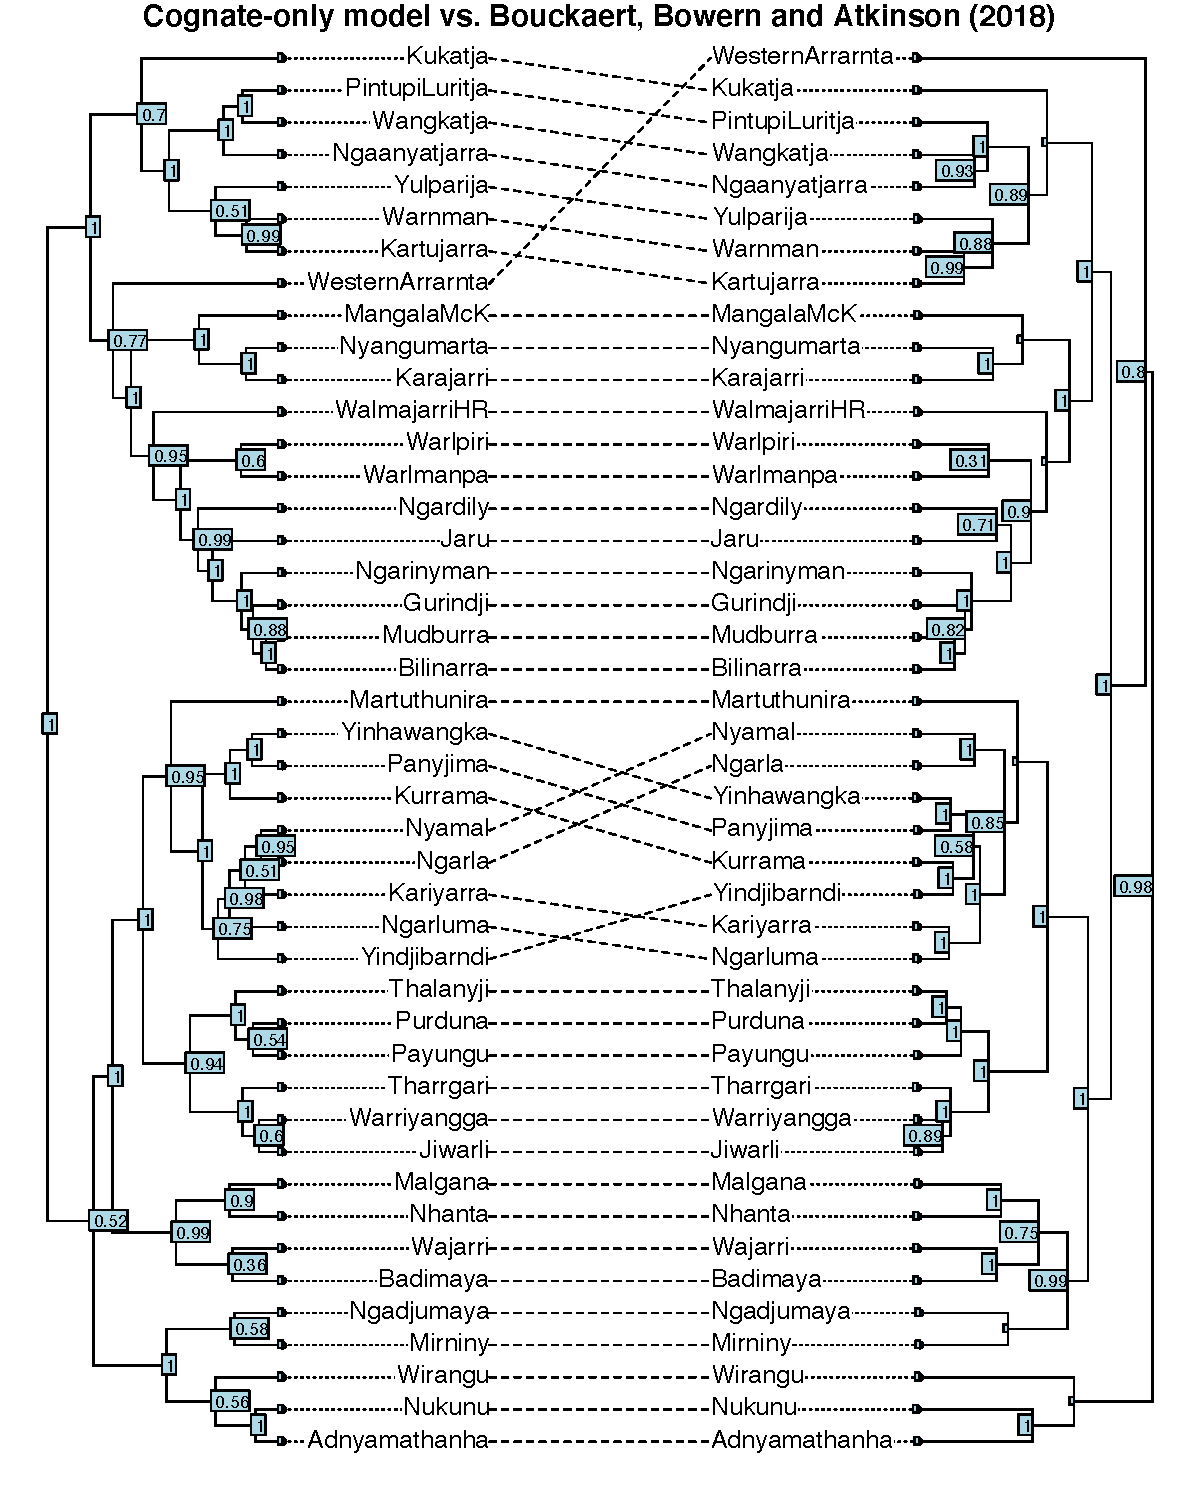
\includegraphics[width=\textwidth]{06-tree-inference/fig/cogs_vs_bba2018.pdf}
\caption[Maximum clade credibility trees of our cognates-only model and the Bouckaert, Bowern \& Atkinson (2018) phylogeny]{\label{fig:cogs-vs-bba2018}The maximum clade credibility trees of our cognates-only model (left) and the Bouckaert, Bowern \& Atkinson (2018) phylogeny (right). Our model aims to replicate the BBA phylogeny as close as possible, although the language sample is restricted and there are some small model and software differences. Overall, the trees are mostly congruent, which gives reassurance that our baseline model is reliable.}
\end{figure}

\hypertarget{main-test}{%
\section{Main test: Tree inference with phonotactic data}\label{main-test}}

\hypertarget{data}{%
\subsection{Data}\label{data}}

There are three main sources of data for this experiment. One is cognate data from \textcite{bouckaert_origin_2018}, to which we apply an evolutionary model following \textcite{bouckaert_origin_2018}, as evaluated in Preliminary Test 2 (Section \ref{prelim-2}). There are two sets of phonotactic data, one binary and one continuous. Binary biphone data, which codes the presence or absence of biphones---sequences of two phonemes---in each language, is included with the best supported evolutionary model evaluated in Preliminary Test 1 (Section \ref{prelim-1}). Finally, we use a dataset of continuous phonotactic characters coding frequencies of transitions between natural sound classes. The data extraction process is detailed further as follows. Each consonant phoneme appearing in our wordlist data is binned into two natural classes, one for place of articulation and one for manner of articulation. Place classes are labial, dental, alveolar, retroflex, palatal and velar. Manner classes are obstruent, nasal, vibrant, lateral, glide, and rhotic glide. For the purposes of this experiment, we group all vowels into a single `vowel' class and also include word boundaries. The choice of place and manner natural classes is based on well-established principles of organisation among segments in Australian languages \autocites{dixon_languages_1980}{hamilton_phonetic_1996}{baker_word_2014}{round_segment_2021}{round_phonotactics_2021}. From each wordlist, we extract the frequency of a sound class \(x\) followed by a sound class \(y\), relativised over all instances of sound class \(x\). For use in BEAST, we logit-transform all the data to move from a 0--1 frequency interval to the real line. To include 0 and 1 frequency values in the logit-transformation, we follow a standard procedure of converting 0 values to \(\frac{min}{2}\), i.e.~half the smallest non-zero value, and converting 1 values to \(0.5 (1 + max)\), i.e.~half way between 1 and the maximum value less than 1. The evolutionary model applied to sound class transition frequency data in BEAST is a simple Brownian motion model which allows character values to wander up or down with equal possibility. We initially considered applying a single multivariate Brownian motion model to all continuous traits, however, the computational memory and time required by a multivariate Brownian motion model scales exponentially as the number of characters is increased. Instead, we fit a Brownian motion model to each character individually. This greatly increases the number of parameters in the overall model and potentially makes it less realistic, but it keeps the project computationally feasible. We return to this topic further in the discussion.

The choice of phonotactic data warrants brief further comment. We select sound class transition frequency data for a few reasons. One is that it partially, though not entirely, accounts for a lack of independence between biphone characters. This is because phonological rules, phonotactic restrictions and historical sound changes typically affect natural classes of phonemes rather than individual phonemes. This is not a perfect solution---sound classes themselves are independent from one another to varying degrees. A second reason is that \textcite{macklin-cordes_phylogenetic_2021} find a stronger degree of phylogenetic signal in sound class transition frequency data compared to transition frequencies between individual phonemes. A third reason is computational. A dataset of continuous characters equivalent in size to the binary biphone dataset would increase the computational time required to run BEAST by orders of magnitude, rendering the study impractical.

The decision to focus on frequency data in particular also warrants further explication. Notwithstanding the computational limitations we encounter, frequency data offers a number of possible advantages for phylogenetic inference. One is that it allows us to capture a finer grained level of information than binary data would allow. Binary data is more similar to the kind of phonotactic information one might find in a published language grammar, where a description of phonotactics that one would typically encounter involves a series of statements on the (binary) permissibility or otherwise of certain combinations of segments or natural classes of segments. This information does not, however, account for quantitative differences between common, high frequency sequences versus disfavoured sequences that rarely arise in a language's lexicon. There is considerable evidence to suggest that speakers are psychologically attuned to these kinds of phonological frequencies \autocites{coleman_stochastic_1997}{zuraw_patterned_2000}{ernestus_predicting_2003}{albright_rules_2003}{eddington_spanish_2004}{hayes_stochastic_2006}{gordon_phonological_2016}. The second reason is that the relatively rapid, semi-automated extraction of transition frequencies from wordlists captures structural variation between languages at a scale and degree of precision that would be difficult to attain from manual data coding methods (as preferred for the coding of lexical cognate data and grammatical data used in previous linguistic phylogenetic work). \textcite{macklin-cordes_phylogenetic_2021} show that this transition frequency dataset contains stronger phylogenetic signal than its binary equivalent. Increasing variation by shifting from categorical-valued characters to continuous characters has also been noted as advantageous for phylogenetics in biology, in the context of anatomical morphological data \autocites{parins-fukuchi_use_2018}{wright_systematists_2019}. An additional advantage is that our method avoids observer bias. We don't have to rely on an expert picking and choosing which parts of a grammatical or lexical system are interesting and worth coding. This has been noted as an advantage of large-scale extraction of continuous morphological characters in biology too \autocite{wright_systematists_2019}. Lastly, since we automatically extract frequencies for all possible biphones, we do not need to correct for acquisition bias or ascertainment bias \autocite{leache_short_2015}.

There is one limitation of the frequency data, which is that the Brownian motion model requires values above 0 and below 1. As described above, 0 values and 1 values are transformed to values very slightly above 0 and very slightly below 1 prior to logit-transformation. The inclusion of binary data in this study as well as frequency data is partly an effort to retain 0 and 1 values, which can be linguistically meaningful. One final limitation is that, throughout, our phonotactic data concerns linear sequences of exactly two segments. This is phonotactics in the simplest sense, and does not directly capture phonotactic restrictions that depend on sequences beyond two segments, syllable structure or morpheme boundaries. Nevertheless, \textcite{macklin-cordes_phylogenetic_2021} confirm that this simple level of phonotactic data is sufficient to detect strong phylogenetic signal.

As mentioned in Section \ref{prelim-2}, we reduce the language sample to 44 western Pama-Nyungan languages. This was necessary to keep the computational demands of the experiment reasonable. We selected the western branch of Pama-Nyungan due to it being relatively well-attested in modern sources compared to those in, for example, the south-east of Australia where language documentation is more often reliant on archival sources due to the disproportionate impact of colonialism in this part of the continent.

We run BEAST on two phylogenetic models: a `linked' model, which contains a single tree likelihood term calculated using all cognate and phonotactic data, and a `separate' model, which contains two tree likelihood terms, one calculated using cognate data only and the other using phonotactic data only (both binary and continuous). We run ten independent MCMC chains of 100 million iterations on each model, inspect and combine the results, estimate marginal likelihoods for each of the `linked' and `separate' models and generate three maximum clade credibility trees (one for the `linked' model, and one each for the cognate-only and phonotactics-only elements of the `separate' model).

\hypertarget{main-results}{%
\subsection{Results}\label{main-results}}

One first observation is that the MCMC process in BEAST tends to get stuck in local optima within the probability space and occasionally fails to converge. When this became clear, we increased the number of independent chains from an initial four to ten. Inspecting the joint probability traces for each of the linked model's ten runs, we find one clearly preferred area of the state space (Figure \ref{fig:linked-all-trace}). We remove two clear outliers stuck in local optima above and below the others. Two additional runs (visible in Figure \ref{fig:linked-all-trace} as two overlapping, slightly bimodal distributions, just to the left of the bulk of other chains) are removed since, although they overlap considerably with the others, they too seem to represent a distinct local optimum in the state space (one of these also failed to reach stable convergence). Three more chains failed to reach stable convergence after a reasonable (10--20\%) burn-in period and had to be removed. This leaves three stable chains with suitably high ESS values and consistent areas of convergence (the three tallest, central peaks in Figure \ref{fig:linked-all-trace}). The combined ESS for joint probability is 196. Over 200 would be preferable but we accept this as marginally acceptable. After discarding 10\% burn-in, we are left with a combined 270-million-state analysis.

BEAST computes two marginal likelihood estimates, one via the path sampling method \autocite{baele_improving_2012} and one via the stepping stone sampling method \autocite{baele_accurate_2013}. In normal operation these two estimates should be roughly equivalent. In this instance, the log marginal likelihood estimates for the combined analysis are 598,885 (estimated via path sampling) and 988,231 (estimated via stepping stone sampling). Currently, it is unclear whether or not these log MLE figures are meaningful. Log MLEs for each individual chain vary between 459,380 and 672,466 which is considerably more variation than we would expect, given that a difference of 20 is generally considered significant. Given that all chains represent the same data and model and converge in approximately the same space, we would expect their log MLEs to be around the same and certainly not as divergent as this. We discuss this further below.

\begin{figure}
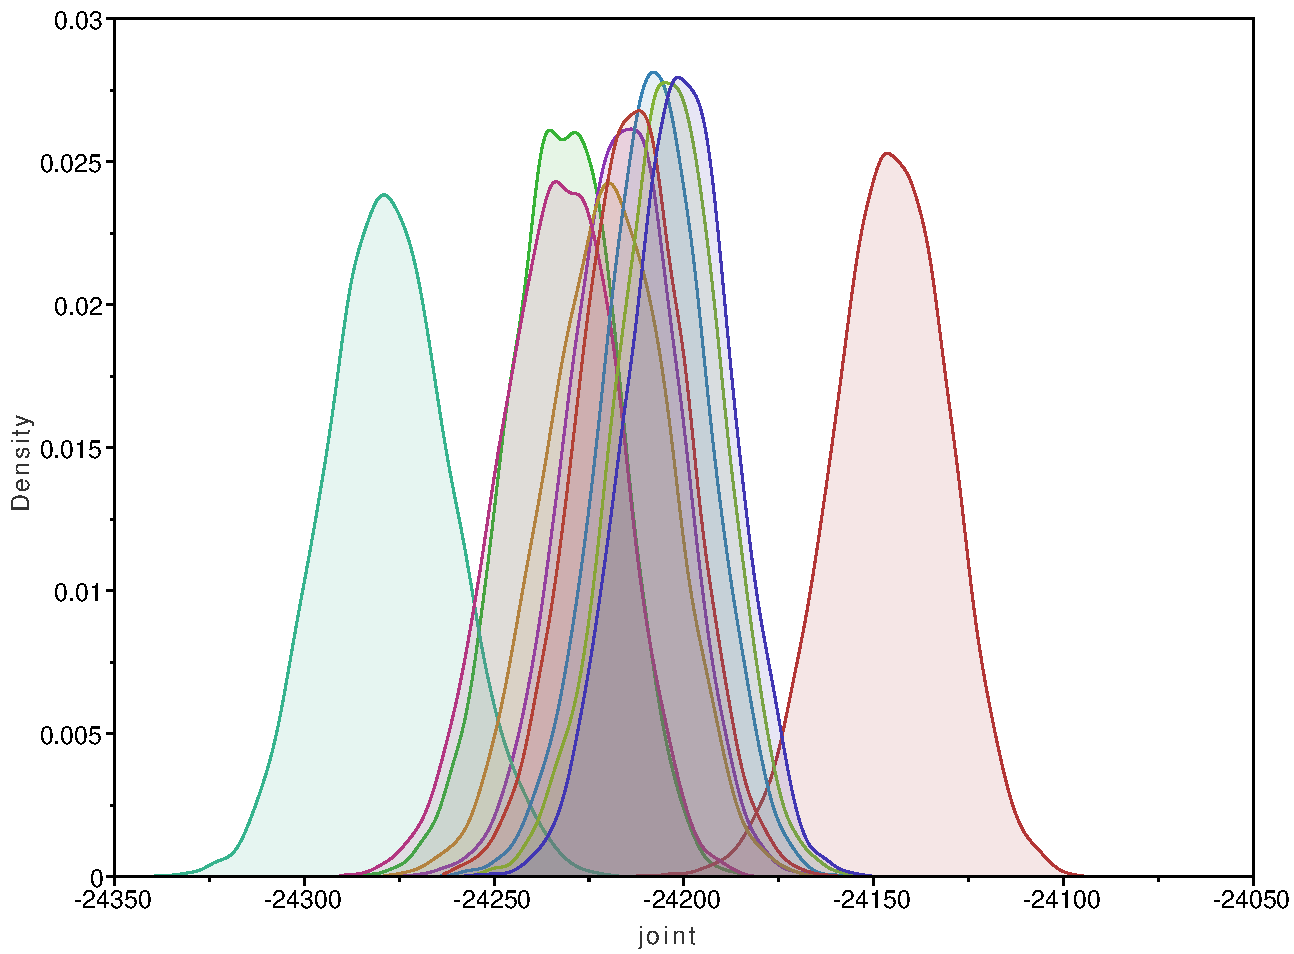
\includegraphics[width=0.5\linewidth]{06-tree-inference/fig/joint_trace_dens_ch1-10} 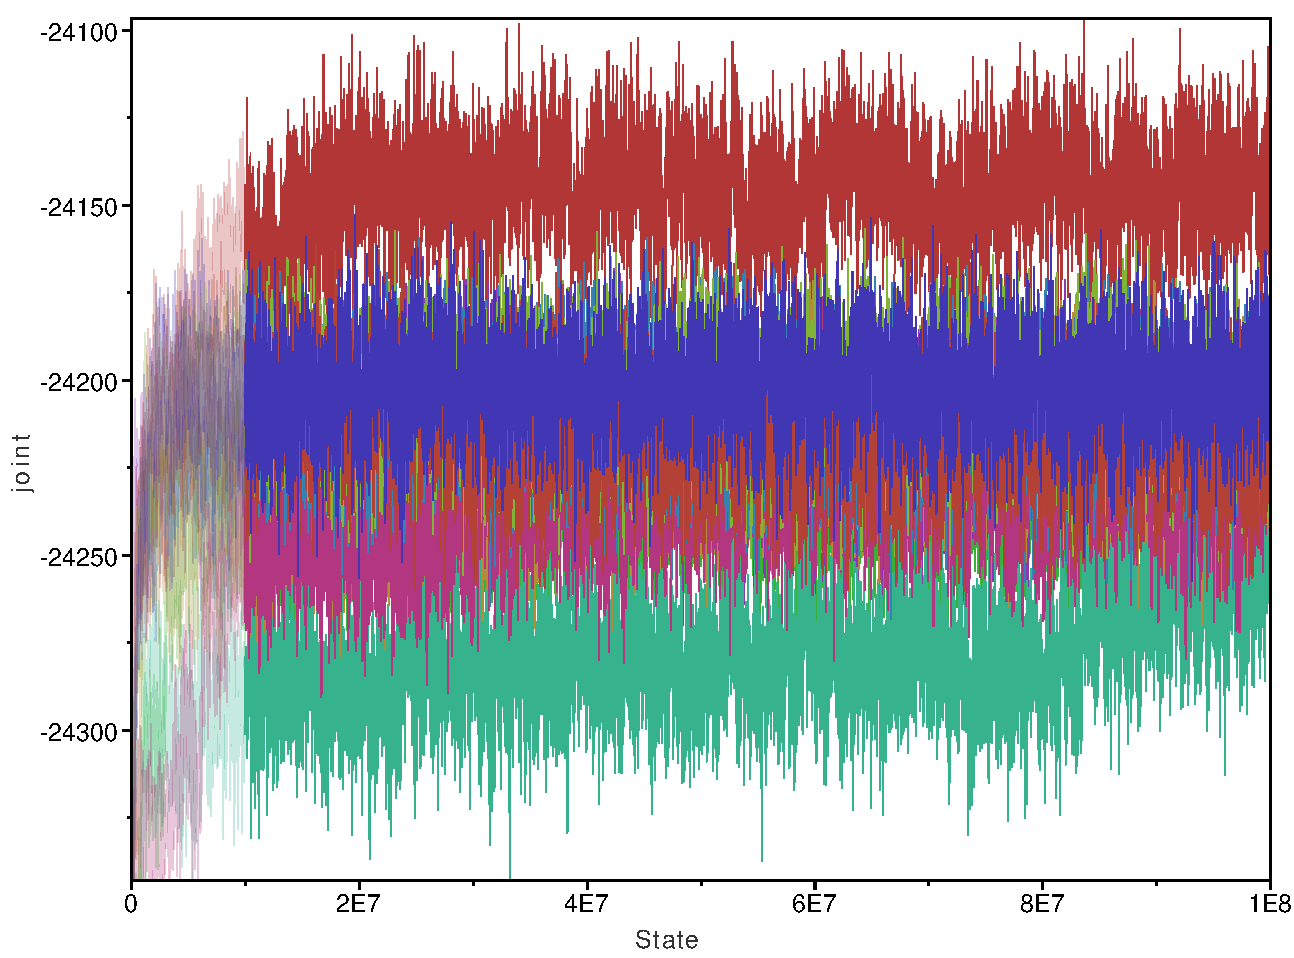
\includegraphics[width=0.5\linewidth]{06-tree-inference/fig/joint_trace_ch1-10} \caption[MCMC joint probability traces for the linked model]{MCMC joint probability traces for the linked model. Although a preferred general area of the probability space emerges, this area has wide bounds. There are two clear outliers and there is a considerable degree of inconsistency between chains.}\label{fig:linked-all-trace}
\end{figure}

The separate model, in which two trees are sampled at each step, one inferred using only cognate data and one inferred using only phonotactic data, fails to reach stable convergence and gives unacceptably low ESS figures in most instances. With a burn-in of 15\%, as per the linked model above, only 3 chains give a stable posterior sample with satisfactory ESS values. A fourth stabilises after a 20\% burn-in, and three others eventually stabilise in similar areas of the probability space to the others, but only after burn-in values of 50\%, 60\% and 70\%. We apply a consistent 20\% burn-in to the four most stable chains and discard the rest. Two of these converge in the same area while the other two converge in spaces of slightly lower joint likelihood. On this evidence, it is not entirely clear which is the most correct posterior distribution. We accept the two higher likelihood chains space as it makes the study's null hypothesis deliberately harder to reject (the null hypothesis that the joint model is no better than the separate model is harder to reject if we raise the bar set by the separate model). This gives a posterior sample of 160 million states and a marginally satisfactory ESS of 100 or greater for all parameters. Maximum clade credibility trees for each of the two tree elements---one inferred only with cognate data and the other inferred only with phonotactic data---are depicted in Figure \ref{fig:separate-cogs-vs-phonotactics-all}.

\begin{figure}
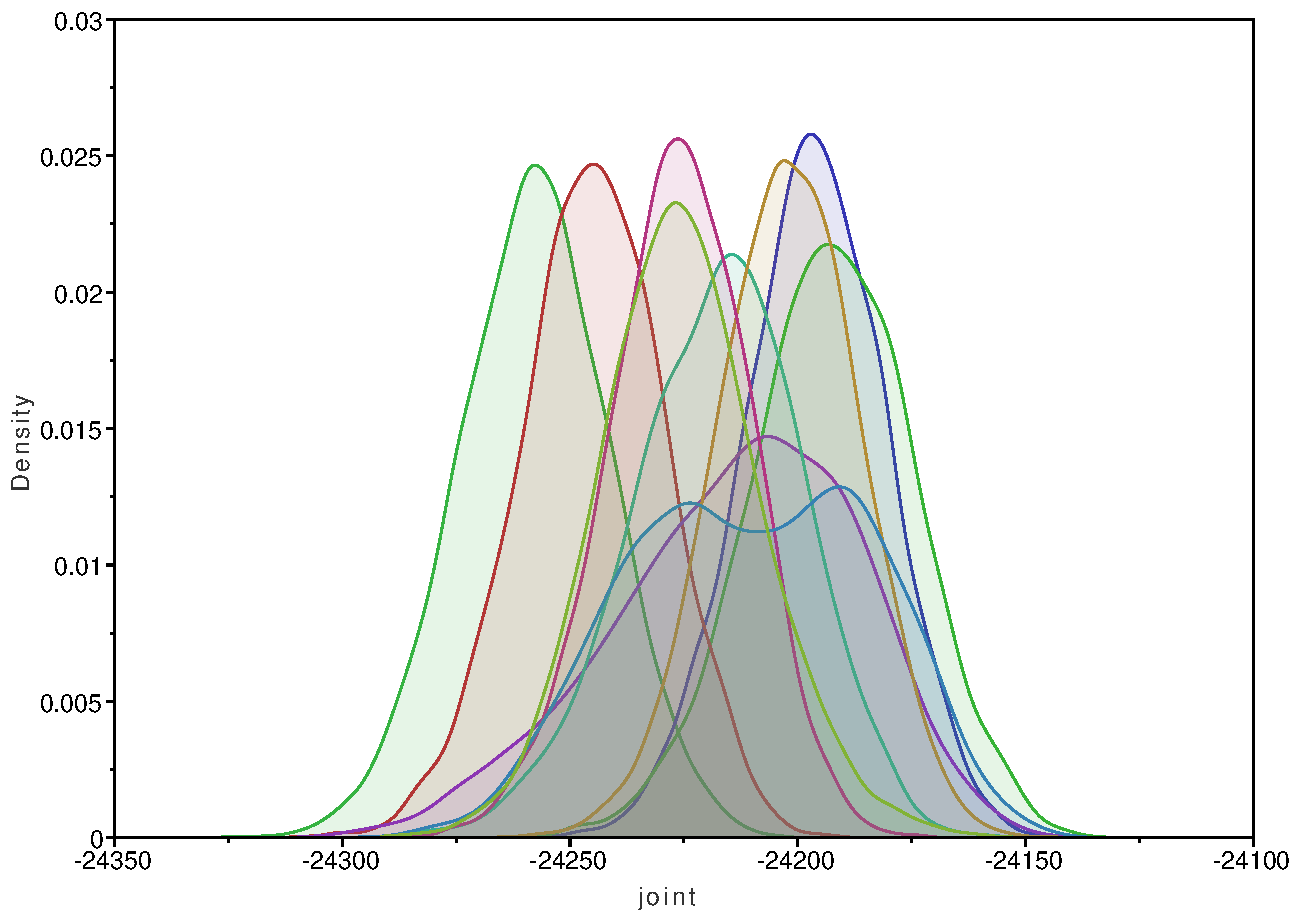
\includegraphics[width=0.5\linewidth]{06-tree-inference/fig/sep_trace_ch1-10} 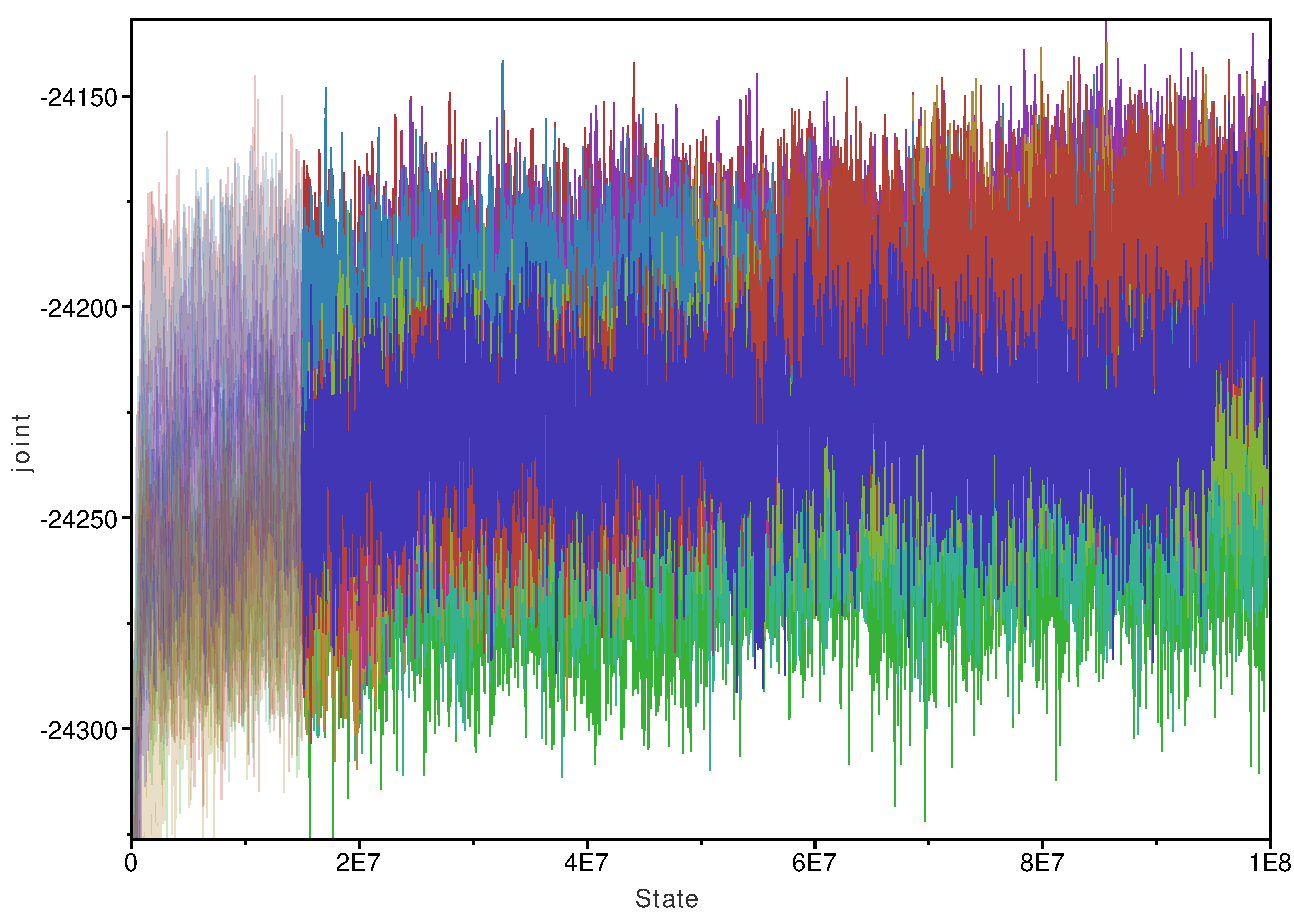
\includegraphics[width=0.5\linewidth]{06-tree-inference/fig/sep_trace_dens_ch1-10} \caption[MCMC joint probability traces for the separate model]{MCMC joint probability traces for the separate model. The lack of consistent (as seen on the left) and stable convergence (as seen on the right) is readily apparent.}\label{fig:separate-all-trace}
\end{figure}

The log MLEs for the separate model are 348,287 (estimated via path sampling) and 568,402 (estimated via stepping stone sampling). These MLEs can be compared with MLEs for the linked model in Table \ref{tab:linked-vs-separate-mles}. The linked and separate models can be compared using Bayes factors, following Equation \eqref{eq:bf}.

\begin{equation}
BF = log(MLE_{linked}) - log(MLE_{separate})
\label{eq:bf}
\end{equation}

The sign of the Bayes factor indicates which model is preferred. Bayes factors testing support for the linked model over the separate model are given in Table \ref{tab:linked-vs-separate-bfs}. Using both path sampling and stepping stone sampling methods, the Bayes factors seem to indicate decisive support for the linked model over the separate model. At face value, these figures are evidence for the hypothesis that including quantitative phonotactic data with more traditional cognate data can strengthen phylogenetic tree inference in linguistics. However, given the extreme divergences between MLE estimates from chain to chain and between MLE inferential methods, this evidence should be considered tentative at best.

\begin{table}

\caption[Marginal likelihood estimates (MLEs) for linked and separate phylogenetic models]{\label{tab:linked-vs-separate-mles}Marginal likelihood estimates (MLEs) estimated via path sampling and stepping stone sampling methods for linked and separate phylogenetic models.}
\centering
\begin{tabular}[t]{lrr}
\toprule
Model & Path & Stepping stone\\
\midrule
Linked & 598,885 & 988,231\\
Separate & 348,287 & 568,402\\
\bottomrule
\end{tabular}
\end{table}

\begin{table}

\caption[Bayes factors indicating support for the linked model over the separate model]{\label{tab:linked-vs-separate-bfs}Bayes factors indicating support for the linked model over the separate model.}
\centering
\begin{tabular}[t]{lr}
\toprule
Method & BF\\
\midrule
Path sampling & 250,598\\
Stepping stone & 419,829\\
\bottomrule
\end{tabular}
\end{table}

Another way to evaluate these results is to consider the topologies and posterior support values of maximum clade credibility trees. In Figure \ref{fig:cogs-vs-linked-all}, we compare the maximum clade credibility tree from the linked model to the maximum clade credibility tree from the cognates-only model discussed in Section \ref{prelim-2}. A first observation is that the linked model posits Western Arrernte as the outermost taxon, branching off first from all other subgroups. This is different to the cognates-only model but in line with \textcite{bouckaert_origin_2018}. Western Arrernte is notable for a couple of reasons. Firstly, in our language sample it is the sole representative of the whole Arandic subgroup. Secondly, in the case of the linked model, it is almost certainly being pushed to the outermost position in the phylogeny by its phonotactics. Arandic languages show evidence of major phonological change prior to proto-Arandic. In this instance, all the other subgroups are being grouped together based on their conservatism, driving Arandic into the outlier position. This is unfortunate, since subgroups should be identified from shared innovations, not shared retentions (as is happening here). This is potentially a weakness of phonotactic characters: Phylogenetic methods rely on there being many changes in order to overcome their inability to directly distinguish innovations from retentions. However, many phonological changes are so rare (relative to the phylogeny being studied) that there is not enough evidence to do this, resulting in this kind of undesirable grouping by shared retention.

The trees are largely congruent although there are some shifts in internal structure in some subgroups. The internal structure of Ngumpin-Yapa shifts once again---the Yapa branch (Warlpiri and Warlmanpa) gets split in the linked model. Overall, there is a general flattening of the tree structure in the linked model, approaching a star phylogeny. One possibility is that the tree structure is being flattened by the addition of the binary phonotactic data. As discussed, this sample of western Pama-Nyungan languages share largely homogeneous phoneme inventories and similar phonotactics in binary, permissibility terms. The binary data is relatively low resolution and might be masking phylogenetically informative variation between languages. That said, for the lower order topological structure that is present, the linked model tends to give good posterior support values, with a couple of exceptions. Perhaps unsurprisingly, Ngumpin-Yapa is an exception with very low support values. Another exception is the subgroup of Warnman, Kartujarra and Yulparija in the Wati clade. In other cases though, the addition of phonotactic data in the linked model seems to strengthen some support values, for example, within the Kanyara-Mantharta (languages listed Purduna--Tharrgari in Figure \ref{fig:cogs-vs-linked-all}) and Kartu (Badimaya--Nhanta) subgroups.

\begin{figure}
\centering
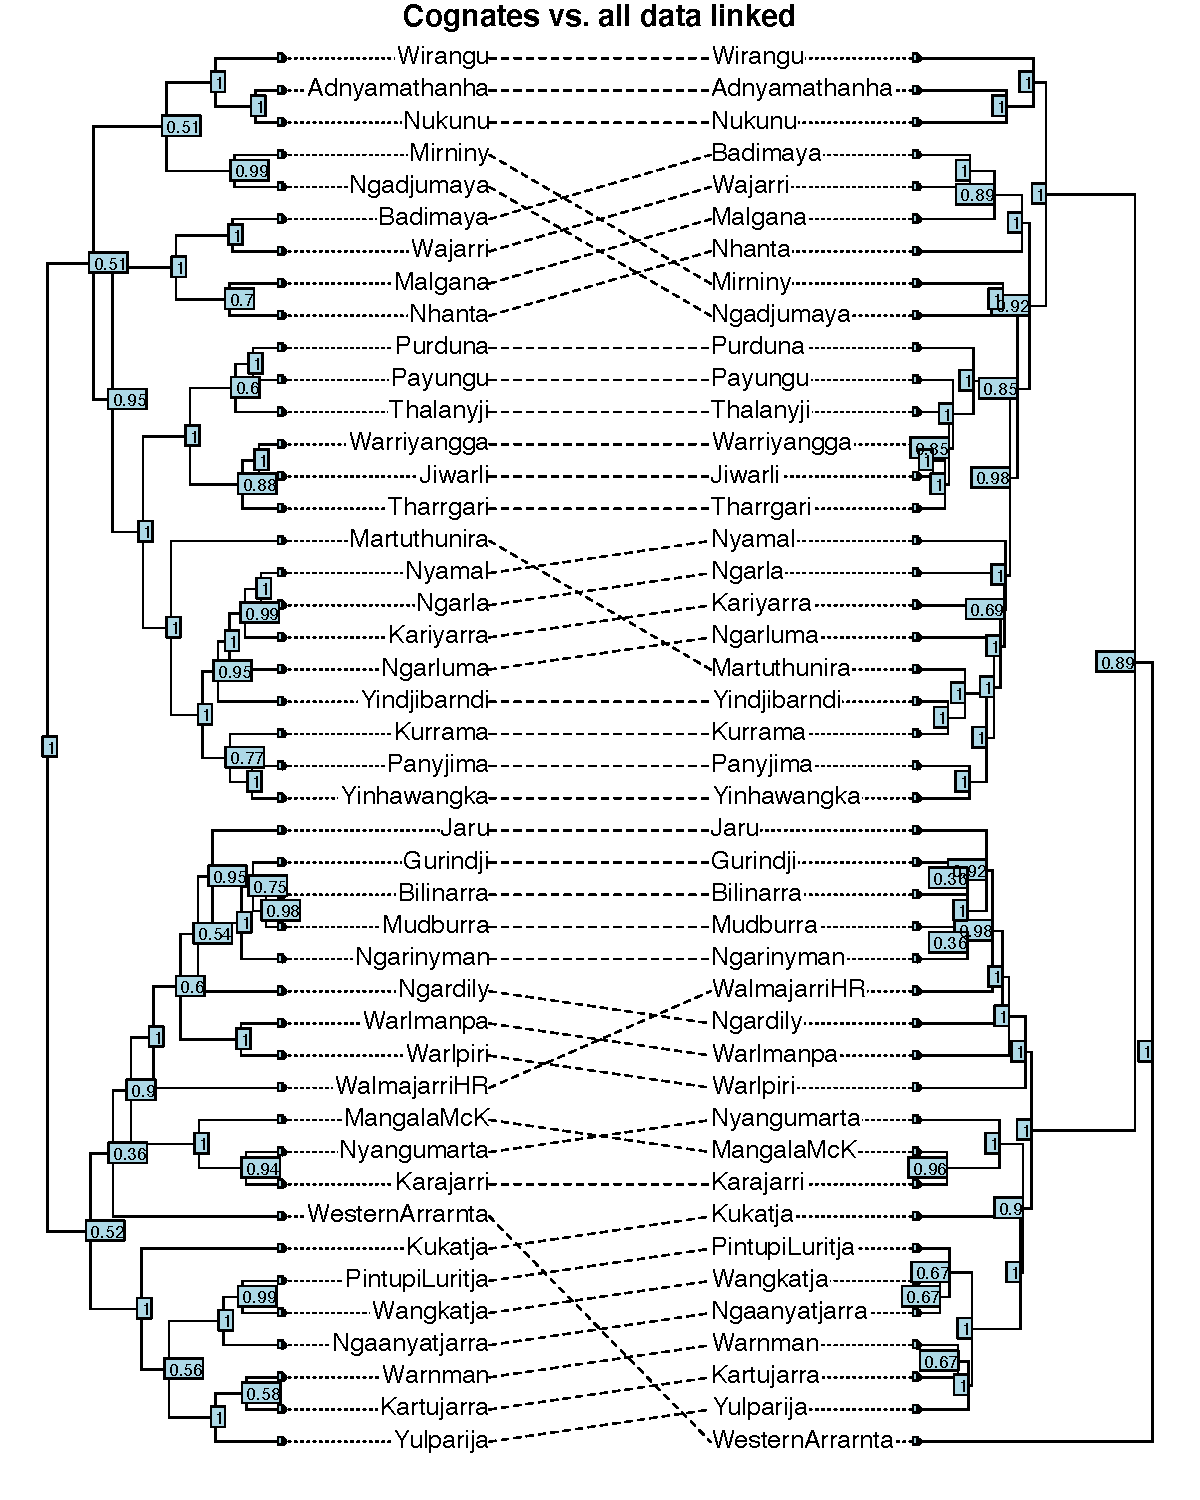
\includegraphics[width=\textwidth]{06-tree-inference/fig/cogs_vs_linked_all.pdf}
\caption[Maximum clade credibility trees for the cognates-only model (from Preliminary Test 2) and the linked model]{\label{fig:cogs-vs-linked-all}Maximum clade credibility trees for the cognates-only model from Preliminary Test 2 (left) and the linked model (right), which was inferred from cognate data and phonotactic data together.}
\end{figure}

The flattening effect of the phonotactic data is evident when MCC trees are calculated for each of the two tree elements of the separate model. Recall that the separate model includes two separate tree elements---one inferred with cognate data only and one inferred with phonotactic data only (both binary and continuous). Maximum clade credibility trees are inferred for each of these elements and plotted in Figure \ref{fig:separate-cogs-vs-phonotactics-all}. Side-by-side, the loss of intermediate tree-like structure is apparent in the phonotactics-only MCC tree. It is perhaps unsurprising then that the linked model, in which a single tree is inferred from all the data together, produces an intermediate level of tree-likeness, less tree-like than the cognates-only model but not as star-like as the phonotactics-only tree in the separate model.

\begin{figure}
\centering
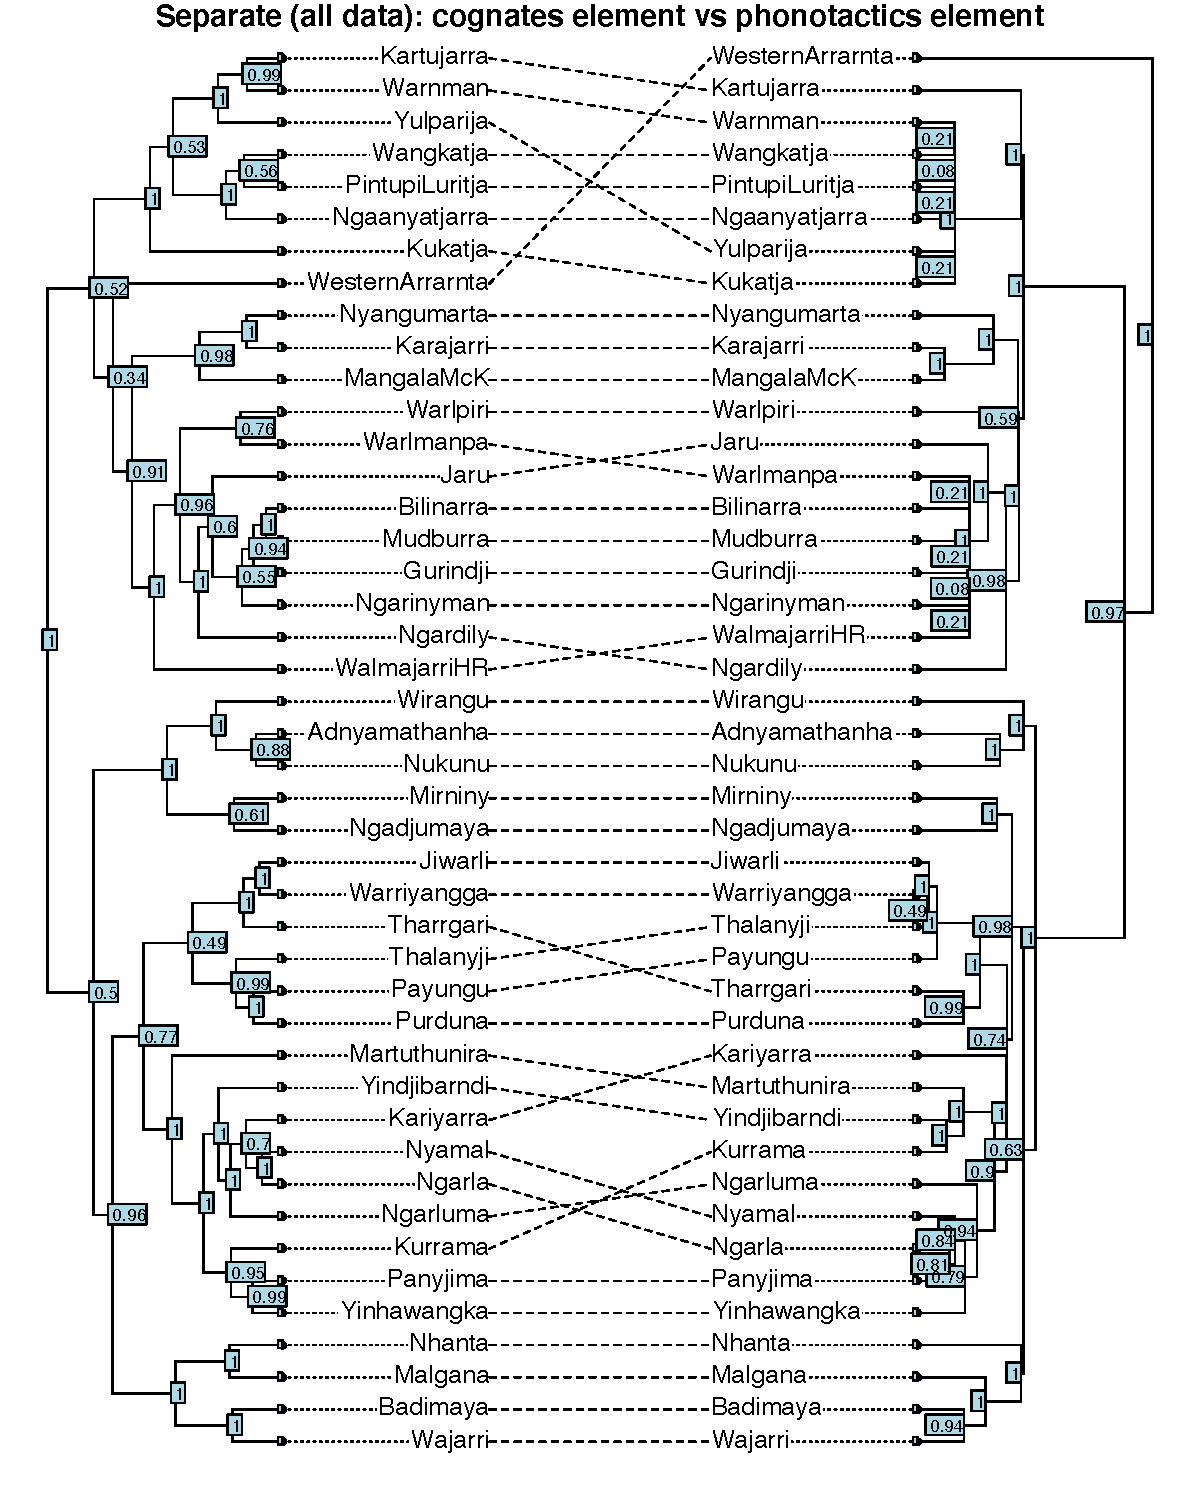
\includegraphics[width=\textwidth]{06-tree-inference/fig/separate_cogs_vs_phonotactics_alldata.pdf}
\caption[Maximum clade credibility trees from the separate model]{\label{fig:separate-cogs-vs-phonotactics-all}Maximum clade credibility trees from the separate model. The tree inferred from cognate data only is depicted on the left, the tree inferred from phonotactics only is on right. The flatter, star-like topology and low clade support values in the tree on the right is suggestive of non-treelike signal in the phonotactics data.}
\end{figure}

\hypertarget{follow-up-test}{%
\section{Follow-up test: Removing binary biphone data}\label{follow-up-test}}

Upon reviewing results of the main test, one initial hypothesis was that the binary biphone data, which we expected would contain a little phylogenetic signal but to a relatively low degree, might be having an outsized influence on likelihood calculations in BEAST. This relatively homogeneous dataset, we reasoned, might be driving star-like tree signal in the tree topologies and increasing uncertainty in the analysis. In the likelihood calculations for our models, each data partition is effectively weighted proportionately to the amount of data within it (not due to a particular analytical decision but just because of the way BEAST is presently implemented). Our models contain 1,097 binary lexical cognate characters and 2,236 binary biphone characters, so the cognate data gets outweighed over 2-to-1 despite our prior expectation that the cognate data should be relatively more informative.

To test this hypothesis, we ran one follow-up test which is a replication of the linked model from the main test but with the binary biphone data removed. That is, the phylogeny is inferred from lexical cognate data and continuous phonotactic data only. We ran four independent 100-million-state MCMC chains in BEAST. Unfortunately, the new linked model does not seem to produce more stable or consistent convergences than the original linked model presented above. Of the four MCMC chains, two fail to reach stable convergence while the other two converge to slightly different optima in the state space. We err on the side of the chain in the lower likelihood space, which also has the most stable convergence and highest ESS values (1,269 for joint probability and \textgreater{}200 for all other parameters). We discard 10\% burn-in and calculate an MCC tree for the remaining sample. This is plotted in Figure \ref{fig:linked-all-vs-linked}, side-by-side with the MCC tree for the main linked model above. As can be seen, the linked model produces practically identical tree topologies regardless of whether the binary biphone data is included or not. Some differences in clade support values can be observed, but in some instances these values increase with the removal of binary biphone data while in other instances they decrease. Overall, these differences in clade support values seem not to favour one particular tree over the other.

We conclude that the presence of a large partition of binary biphone data in the main study was not unduly impacting likelihood calculations and the MCMC process. The results are largely replicated whether or not this dataset is included in the study.

\begin{figure}
\centering
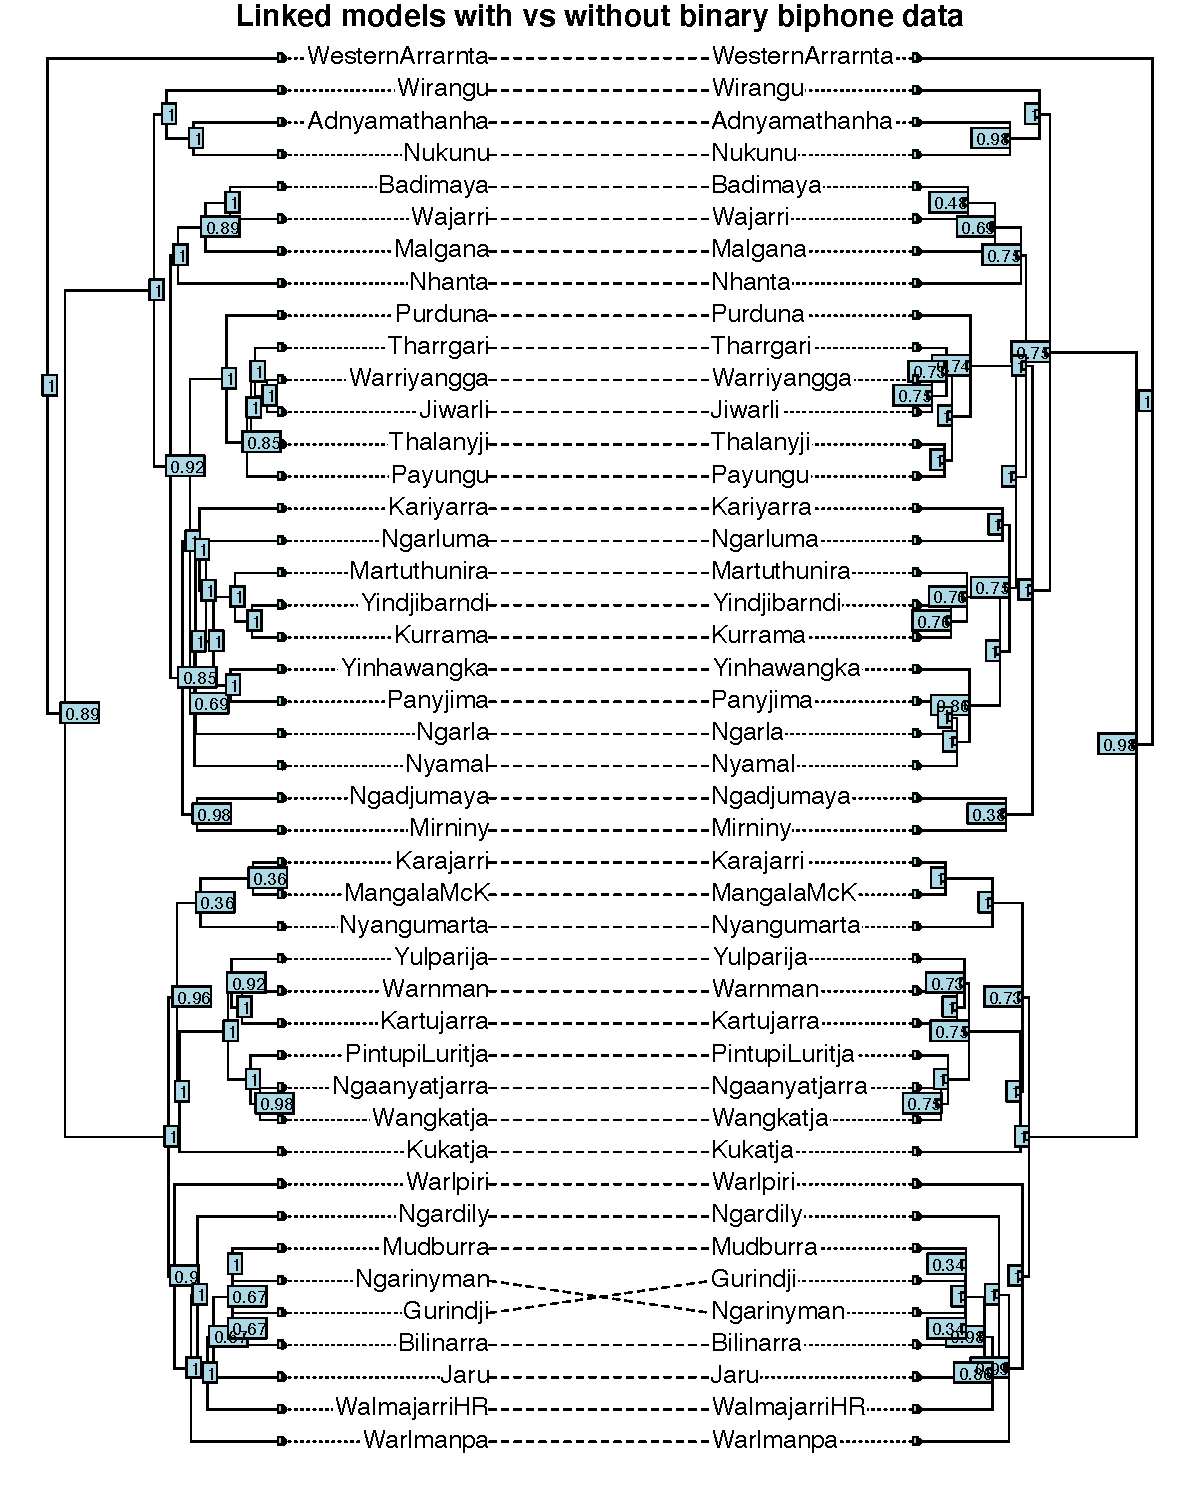
\includegraphics[width=\textwidth]{06-tree-inference/fig/linked_all_vs_linked.pdf}
\caption[Maximum clade credibility trees from the linked model in the Main Test and a follow-up model]{\label{fig:linked-all-vs-linked}Comparison of maximum clade credibility trees from the linked model in the Main Test (left) and a follow-up model which includes cognate data and sound class frequency data, but excludes the binary biphone data. Both trees appear highly congruent, suggesting the binary biphone data had relaively little effect on the results of the Main Test.}
\end{figure}

\hypertarget{pn-tree-discussion}{%
\section{Discussion}\label{pn-tree-discussion}}

In this study, we sought to test the question of whether phonotactic data could help strengthen the inference of phylogenetic signal, when included in a Bayesian computational phylogenetic model in conjunction with more traditional, lexical cognate data. We were motivated by earlier findings that phonotactic data, represented here by binary characters coding the presence or absence of biphones and continuous characters coding the frequency of natural sound classes being followed by other sound classes in biphone sequences, contain phylogenetic signal \autocite{macklin-cordes_phylogenetic_2021}. Our method of testing this hypothesis was to develop two phylogenetic models, a `linked' model and a `separate' model, and infer phylogenies for each using a Bayesian MCMC process implemented in BEAST. In the linked model, tree likelihoods are calculated at each step using existing lexical cognate data from \textcite{bouckaert_origin_2018} and both binary and continuous phonotactic data. In the separate model, two tree likelihoods are calculated, one using cognate data and the other using phonotactic data separately. Marginal likelihoods are estimated to give an indication of overall support for each model. Maximum clade credibility trees are calculated to compare tree topologies and support for particular subclades.

Our results do not support the hypothesis that a better supported phylogeny could be inferred with phonotactic data. To the contrary, we found that the addition of phonotactic data contributed instability and uncertainty into the MCMC process. We also found the MLE process to be unreliable, with extreme divergences between even chains that seemed to reach stable convergence in the same probability space. Inspecting the maximum clade credibility trees, the linked phylogeny seemed to produce an MCC tree broadly comparable to the equivalent phylogeny produced from cognate data only. However, the internal structure of some subgroups did get altered, the posterior clade support values did not, on the whole, improve, and there seemed to be a degree of star-like flattening of the tree shape. To the extent that the linked model recovered the topology of the cognates-only phylogeny, it might be said that it did so in spite of apparent star-like signal in the phonotactic data, rather than with the assistance of phonotactic data. The conclusion is that phonotactic data, in the form presented here, does not strengthen phylogenetic tree inference, at least within the present statistical and computational implementation.

The next question is to what extent these findings represent a genuine negative result, i.e.~evidence for a more general conclusion that phonotactic data does not strengthen phylogenetic tree inference. If this is the case, then future linguistic phylogenetics research should abandon phonotactics as a potential data source. The alternative, however, is that the negative result is attributable to any combination of issues with data acquisition and/or experimental design. In this case, we cannot say the study supports any particular insight into the phylogenetic dynamics of phonotactic systems in human language. Rather, we would require further study, hopefully benefiting from the lessons of the present attempt, before making any conclusions either way. There are reasons, as discussed in the paragraphs that follow, to suspect that this study is an instance of the latter. If that is correct, then the current experiment is best interpreted not as evidence against any particular hypothesis, but rather as evidence for the need for further refinement along the lines we discuss below.

The following points of discussion fall under two main umbrellas. We start with more technical issues relating to experimental design and implementation, then follow with more general, theoretical matters. Firstly, we must consider the difficulties we observed achieving stable, consistent convergences between MCMC chains. It is possible that the development of relatively simple technical fixes might help rectify this issue to some degree. Although 100 million states seems to be enough to reach normal, stable convergence for many chains in this study, others fail to converge or, in some instances, get stuck for a while before managing to escape a local optimum and converging somewhere else very late in the chain. The most obvious solution to this is to try running much longer chains. The difficulty here is operating within computational constraints, as continuous characters increase the running time of the MCMC process by orders of magnitude. The issue of computational feasibility is compounded again as the size of the phylogeny increases. It would be challenging, for example, to run even our present 100 million state chains if we extended our model to the 112-language Pama-Nyungan sample we used in Section \ref{prelim-1}. One second technical fix would be to adjust the operators in BEAST that govern how parameter values shift from state to state. Allowing larger jumps in the parameter space could help the MCMC chain to escape local optima.

A more complex technical issue is the implementation of an evolutionary model for continuous characters. When working with binary datasets in phylogenetic software, one would usually work with a single data partition containing all binary characters or a small number of data partitions. The problem with continuous characters is that the computational time and memory demands of a continuous data partition expand exponentially as the number of continuous characters increases. For example, the sound class biphone dataset that we use in this study would take several years rather than several days to run on identical computing hardware, if implemented as a single data partition. To get around this, we created an individual data partition for each individual character. This brought the study into the realm of reality from a practical standpoint, but at the cost of hugely increasing the number of parameters that form part of the model, because individual rates of evolution and likelihood scores had to be inferred for every character. Besides the question of whether treating each character as its own element in the model is realistic (which we address more below), having such a great array of parameters to estimate likely contributes to uncertainty in the analysis. Future study should consider some option in between the extremes of a single data partition and individual data partitions for all continuous characters. The question is how continuous characters should be partitioned and on what basis. One option is to pre-define data partitions on some linguistically meaningful basis (for example, perhaps grouping characters by the sound class of the first biphone segment). The other option is to infer how the data should be partitioned as part of the analysis. There is work in this space using phylogenetic factor analysis, under active development \autocites{tolkoff_phylogenetic_2018}{hassler_inferring_2020}, and this could be explored in the context of large linguistic datasets of continuous variables in future work. Addressing this issue will have the added benefit of addressing the lack of independence issue.

There are other limitations to the evolutionary model for continuous characters that we used. For one, we use a simple Brownian motion model which allows characters to wander up or down with equal probability. This model has the advantages of being straightforward to implement with existing software and also aligns with earlier work by \textcite{macklin-cordes_phylogenetic_2021}. But it also fails to fully encapsulate the way that biphone frequencies are likely to change over time. One question to consider is what a more realistic model of evolution would look like for frequency-based phonotactic characters. To answer this, we need to think about the causal forces of language change that shape these frequencies. We note two such forces here. The first is the introduction of new vocabulary to a language via lexical innovation or borrowing. Each new word entering a lexicon will alter minutely the frequencies of biphone transitions in the language (similarly, transition frequencies will decline as words are replaced or fall out of usage). This is the kind of gradual accumulation of changes that we might expect to follow a Brownian motion-like pattern of evolution (although maybe the rates of going up and down are not equal). Further, since speakers show a preference for high frequency phonotactic sequences over low frequency sequences when coining new words, we might expect this accumulation of changes to follow some a kind of `rich-get-richer' preferential attachment process which would result in the kind of skewed frequency distributions that we observe. Also, when languages borrow vocabulary, the trend is for foreign words with disfavoured phonotactic sequences to shift towards more natively preferred patterns (sometimes gradually over a long period of time, e.g.~in some French borrowings in English, stress has shifted to English pattern but not yet in others; see also \textcite{crawford_adaptation_2009} on Japanese), which would strengthen this kind of preferential attachment process and also keep phonotactic frequency data historically conservative. The second major force on biphone frequencies is regular sound change. We would expect regular sound changes to result in sudden jumps in the frequencies of affected biphones, sometimes to 0 or 1. For example, if a language includes heterorganic nasal+stop sequences that subsequently undergo place assimilation, this will result in a sudden jump, rather than a gradual drift in frequencies from heterorganic nasal+stop sound class characters to their homorganic counterparts. Our binary characters capture some of these effects to a limited extent. For example, in the place assimilation example above, certain biphones will switch from `1' to `0'. In other instances, sound changes could cause characters to switch from missing all together to some non-missing value or vice versa. For example, if a contrastive vowel length distinction emerges, certain biphones (those with long vowels) will go from being a gap to `1' in the binary biphone data for that language. In the case of a merger between short and long vowels, the opposite will be true. Our model, at present, does not obviously account well for regular sound change. One option for addressing this in future work may be to include a Lévy process in the model, which allows for gradual drift punctuated by sudden jumps \autocite{uyeda_rethinking_2018}. One final limitation to note is that the frequency data and evolutionary model in this study do not account for measurement error. Wordlists are necessarily a limited representation of the complete, true lexicon of a language, and so particularly in the case of shorter wordlists, there may be a margin of error between the true frequencies in the language and the frequencies we extract from its wordlist. There is evidence to suggest that accounting for measurement error could help improve results \autocite{round_clouded_2019}. Overall, future work will need to consider more carefully how a realistic evolutionary model for continuous characters should be designed and, if necessary, do the heavy lifting of implementing the model in phylogenetic software rather than relying on currently available implementations. Furthermore, more careful re-evaluation of the frequency distributions of phonemes in \textcite{macklin-cordes_re-evaluating_2020} should be replicated at the biphone level.

Any statistical model is necessarily an abstraction of reality. The challenge is striking the right balance between a model that is realistic enough to produce realistic outcomes and abstract enough to be both practical and generalisable. In this study, we may have compromised on the realism of the model too much in order to keep the project computationally feasible with presently available software and hardware. Technological advances in central and graphical processing units and increased computational parallelisation \autocite[e.g.][]{holbrook_massive_2020} will mitigate this dilemma somewhat in future, but additional work will be required to create evolutionary models that are more faithful to the real-world diachronic processes that generate phonotactic frequencies.

A final point is that future research might consider whether phonotactic data has a role in phylogenetic tree inference or some other aspect of linguistic phylogenetics beyond tree inference itself. In biology, there is ongoing debate on whether morphological data is best suited to a ``simultaneous'' approach, where the tree is inferred jointly from morphological and genomic data, versus a ``scaffolding'' approach, where the tree is inferred from genomic data only, then morphological data is used to investigate other phylogenetic questions (e.g.~dating branching events using morphological data from the fossil record) while being constrained to the genomic tree's topology \autocites{de_queiroz_including_1996}{lee_morphological_2015}. We do not take up the topic further here, but an analogous discussion could be had in linguistics. It may be the case that phonotactic data or some other kinds of linguistic data are better suited to a scaffolding-type approach, playing a role in phylogenetic investigations but only through application to a phylogenetic tree topology that has already been inferred using cognate data.

\hypertarget{pn-tree-conclusion}{%
\section{Conclusion}\label{pn-tree-conclusion}}

Following earlier findings that phonotactic data contains phylogenetic signal, we sought to create and evaluate evolutionary models for two basic representations of phonotactic information for a sample of 112 Pama-Nyungan languages---binary biphone data coding the presence or absence of biphones in a lexical wordlist, and sound class biphone frequency data coding the frequencies of forward transitions between sound classes in a lexical wordlist. Subsequently, we attempted to infer a phylogeny of a subset of 44 Pama-Nyungan languages representing the western branch of the family, using phonotactic data in combination with existing lexical cognate data. Although marginal likelihood estimates on their face seem to support a linked model where the phylogeny is inferred jointly from phonotactic and cognate data, over a separate model where separate trees are inferred from phonotactic and cognate data separately, we find that the calculation of these figures is unreliable in this instance. Further, through comparison of maximum clade credibility trees for the linked model versus a cognates-only model, we find that the addition of phonotactic data does not seem to strengthen posterior clade support values. To the contrary, the phonotactic data seems to introduce a modest star-like signal to the phylogeny, leading to a slightly flatter tree structure.

These results, we argue, are likely the result of oversimplifying the model of continuous phonotactic character evolution and introducing too many free parameters to the model in an effort to achieve computational feasibility and operate within the bounds of existing phylogenetic software. Future research should develop the phonotactic evolutionary model further before re-evaluating its place in the task of phylogenetic tree inference. The first step of this process would be to evaluate empirically the frequency distributions of biphone characters and attempt to link them to causal processes (e.g.~mergers and splits of phonemic categories). Secondly, the Brownian motion model of character evolution would be replaced with a model that incorporates the identified frequency distribution from the previous step and allows character values to move in ways consistent with the causal processes. Thirdly, dependencies and correlated evolution between characters would be identified and the dataset partitioned accordingly. Fourthly, matters of the technical implementation and MCMC convergence process would be addressed, perhaps with advances in GPU parallelisation, with the aim of inferring reliable marginal likelihood estimates.

As linguistic phylogeneticists look beyond the cognate for sources of novel insight, we advocate a methodical progression and thorough methodological evaluation, from language change processes to large-scale linguistic evolution.

% ***************************************************


%CHAPTER 7
% ***************************************************
% Discussion
% ***************************************************
\chapter[Towards phylogenetic phonotactics]{Towards a phylogenetic phonotactic research program}
\label{ch-discussion}

% ********* Enter your text below this line: ********
The motivating research question posed at the start of this thesis was whether or not phylogenetic tree inference could be strengthened by complementing traditional, lexical cognate data with phonotactic data. Given the indeterminate results of the previous chapter, the answer to this question remains elusive. However, there is still much to be gleaned from this experience and general lessons that can be applied to future quantitative interrogations of novel data sources in historical linguistics. This chapter begins with a brief summary of each of the previous chapters, followed by an explanation of how the four separate studies presented cohere into a step-wise interrogation of a novel data source, phonotactics, in linguistic phylogenetics. I present the novel insights that can be drawn from this evaluation. Follow that, I address limitations of the thesis. I turn attention to future research directions and point to possible solutions to limitations that could be pursued in subsequent study. I note how the scope of this present work could be expanded to cover the Sahul continent and the challenges associated with this. Finally, I sketch an outline of the future of methodological development in linguistic phylogenetics and propose a research paradigm in which this could be done.

\hypertarget{discussion-intro}{%
\section{Summary so far}\label{discussion-intro}}

The preceding five chapters began with a literature review followed by four papers (three experimental studies and one research essay). The first paper presented a critical re-evaluation of frequency data in phonology, starting at the most basic level of individual phoneme frequencies. The second examined the role of phylogenetic comparative methods in linguistics and presented some use cases for measuring phylogenetic signal. The third, put those methods for measuring phylogenetic signal into practice, detecting significant phylogenetic signal in phonotactic data. The fourth inferred a Pama-Nyungan phylogeny using phonotactic data combined with and separately from previously published lexical cognate data. I now briefly recapitulate the journey so far.

Chapter \ref{ch-lit-review} critically examined the history of phylogenetic thinking in linguistics and the burgeoning subfield of linguistic phylogenetics. One limitation of linguistic phylogenetic tree inference presently is an over-reliance on lexical data. A relatively restricted number of studies have tried inferring trees with typological characters \autocites[e.g.][]{dunn_structural_2005}{dunn_structural_2008}{sicoli_linguistic_2014}, but these tend to suffer from a limited amount of data \autocite{yanovich_phylogenetic_2020}, logical dependencies between characters \autocite{yanovich_phylogenetic_2020} and rapid evolutionary rates and homology within a restricted state space \autocite{greenhill_evolutionary_2017}. Linguistic phylogenetics stands to benefit from an increased volume of data, including data drawn from a more diverse selection of parts of human language. Separately, with regards to phylogenetic methods themselves, it is recognised that language evolution is not directly analogous to biological evolution and thus linguistic evolutionary processes warrant methodological consideration in their own right. Furthermore, as the discussion in Chapter \ref{ch-pcms} emphasises, linguistic phylogenetics commands its own position in evolutionary sciences. Linguists should not be seen to be rushing to catch up to biologists by taking off-the-shelf methods from a more mature field. There is a great deal of scope for adapting biological tools and methods for inferring linguistic evolution, since biological and linguistic evolution share certain similarities in evolutionary processes. But this should be done by firstly building a ground-up understanding of linguistic evolutionary processes. In this spirit, I seek to evaluate the utility of phonotactic data in linguistic phylogenetics in this thesis, in particular the frequencies of biphones---sequences of two phonological segments.

Chapter \ref{ch-phon-freqs} presented the first of a four-part investigation. The output of a phylogenetic methodology is only as good as the data fed to it. Before simply pouring frequency statistics into a phylogenetic algorithm, I first examined the nature of phonological frequencies and the causal processes that the shape of those frequencies represents. Previous literature has looked at the frequencies of phonemes in particular languages and found that they tend to form heavily skewed distributions (such that there are a few high frequency phonemes and a long tail of many low frequency phonemes), though not skewed in a way that is well described by Zipf's law, which characterises word frequencies. I also found, however, that phoneme frequencies warranted a re-evaluation in light of advances in statistical methods for identifying distributions and demonstrations showing that previous methods were unreliable \autocite{clauset_power-law_2009}. In addition, previous studies tended to be dominated by European languages and Australian languages were either absent or dramatically underrepresented. I used the maximum likelihood framework suggested by \textcite{clauset_power-law_2009} to evaluate the distributions of phoneme frequencies in the lexicons of 166 Australian languages. I found weak support for a Zipfian-like power law structure among more frequent phonemes (though perhaps also a lognormal structure) and weak support for a geometric (or exponential) structure among less frequent phonemes. In the subsequent discussion in Chapter \ref{ch-phon-freqs}, I offer some tentative comments on causal processes. These comments remain speculative, because of the inherent uncertainty in fitting distributions to 20--30 observations (the number of unique phonemes in a given language). However, exponential distributions may be linked to birth-death processes and power law distributions may be linked to preferential attachment processes.

In Chapter \ref{ch-pcms}, I break from discussions phonological data and turn attention to phylogenetic methodologies in comparative study. Phylogenetic methods might be most immediately associated with phylogenetic tree inference in historical linguistics. However, phylogenetic thinking is essential in all comparative fields of linguistics. As Chapter \ref{ch-pcms} demonstrates, phylogenetic effects have long been a consideration in linguistic typology and also comparative biology where, similar to linguistic typologists, biologists are not immediately concerned with the task of tree inference but must consider historical relatedness as a confounding factor in their results. Both fields share similarities but also significant differences in how they deal with phylogeny as a confounding effect in comparative study, more properly termed phylogenetic autocorrelation. I argue in favour of the uptake of phylogenetic comparative methods in linguistics, in which phylogenetic information is incorporated directly into the statistical model. The critical advantage of this approach is that it enables a comparative study to include a maximal amount of data and the maximal extent of existing phylogenetic knowledge. This is in contrast to methods that involve discarding languages in order to create a phylogenetically balanced sample, and/or making limited phylogenetic assumptions, e.g.~assuming equal phylogenetic distance between subgroups of languages in a sample (effectively assuming a star-like phylogenetic structure). Phylogenetic comparative methods require pre-existing phylogenies of languages to implement. Crucially, however, it is possible to use limited phylogenetic information (i.e.~trees that are not fully resolved into bifurcating branches) and it is possible to incorporate phylogenetic uncertainty. And, as I argue, it is better to incorporate some phylogenetic information even if not perfect, rather than neglect phylogenetic autocorrelation altogether and effectively, perhaps unwittingly, assume a star phylogeny. One other use of phylogenetic comparative methods is to evaluate various questions of evolutionary dynamics, as I went on to demonstrate in Chapter \ref{ch-phylo-signal}.

Chapter \ref{ch-phylo-signal} quantifies the phylogenetic information content in phonotactics, a novel data source which has hitherto not featured in linguistic phylogenetic tree inference. I implement offshoot methods of the phylogenetic comparative methods discussed in the previous chapter to measure phylogenetic signal---the tendency of more closely related languages to resemble one another more than more distantly related languages. I extract phonotactic data at the most simple, basic level, firstly by coding the presence or absence of biphones and secondly by extracting biphone transition frequencies from 112 lexicons of Pama-Nyungan languages, corresponding to 112 tips in Claire Bowern's Pama-Nyungan phylogeny. I found a statistically significant degree of phylogenetic signal in all datasets, but particularly strong signal in frequency data, which provides a finer-grained level of information than the relatively low-yield binary data. This result demonstrated the potential utility of phonotactic data in phylogenetic tree inference, which is perhaps contrary to what one might have expected given the ostensibly high degree of phonotactic homogeneity among Australian languages.

Following on from the conclusions of Chapter \ref{ch-phylo-signal}, in Chapter \ref{ch-tree-inference} I present the first instance of phylogenetic tree inference with the addition of the biphone data evaluated in the previous chapter. I combine the binary biphone dataset and biphone frequency transition dataset with a partition of lexical cognate data from \textcite{bouckaert_origin_2018}. For an evolutionary model of lexical cognates, I reproduce as close as possible the model that \textcite{bouckaert_origin_2018} found to be best supported. I use a simple Brownian motion model of evolution for logit transformed biphone frequency data. For binary biphone data, I run an independent preliminary test of 16 different iterations of several evolutionary parameters and then use the best supported iteration as the evolutionary model for this data partition in the main study. Finally, I calibrated the age of the Wati subgroup and overall age of the tree to the date ranges best supported in \textcite{bouckaert_origin_2018}. I then inferred Pama-Nyungan phylogenies using a Markov Chain Monte Carlo (MCMC) process twice. In the first run, the Pama Nyungan tree was inferred jointly from cognate and phonotactic data. In the second run, trees were inferred from cognate data and phonotactic data separately. After discarding an initial burn-in period, a stepping stone process \autocite{baele_accurate_2013} was used to estimate an overall marginal likelihood for each analysis and, from this, a Bayes Factor was calculated to test whether the cognate-phonotactics model produced a significantly better supported tree. This would be evidence for the hypothesis that Bayesian computational inference of linguistic phylogenies can be improved by including partitions of phonotactic data with more traditional lexical cognate data. Unfortunately, these models fail to reach consistent convergence within current computational limitations, and the marginal likelihood estimates prove to be unreliable.

Altogether, the results of these papers demonstrate that large volumes of phonotactic information can be extracted from language wordlists. We hypothesise that the distribution of this phonotactic information is the outcome of diachronic processes and demonstrate that the that the data pattern phylogenetically. That would suggest that the phonotactic data could strengthen phylogenetic tree inference, however implementing it remains challenging. Besides interrogating phonotactics specifically, this thesis illustrates a step-wise procedure for evaluating the utility of other kinds of linguistic data from other parts of language in phylogenetic tree inference. This study is not an attempt to add novel data into a phylogenetic black box and see what happens. The risk of a black box approach is summed up by the old adage `junk in, junk out'. In any results, it would be difficult to discern novel insights from artefacts of the data or unexpected interactions between the data and intricacies of the model and its assumptions. It is possible that this kind of approach may have contributed to a shortcoming of linguistic phylogenetics over the past two decades. That is, although phylogenetic studies have contributed a great deal of new information on questions that historical linguistics had not yet solved, e.g.~detailed internal branching structure within families/subgroups, no one yet has been able to increase the time-depth of existing historical linguistic methods and infer novel macrofamilial relationships. Even as the field of linguistic phylogenetics matures, much of the present work focuses on demonstrating the validity of the method by reproducing existing historical linguistic results. This might be due, in part, to a lack of understanding of what it really means when the output of phylogenetic methods diverges from existing knowledge and whether this constitutes genuine novel insight or some kind of noise. In contrast to the above `junk in, junk out' scenario, I have attempted in this thesis to present a careful, considered, ground-up evaluation of the data and methods before attempting to infer a phylogeny with phonotactic data in Chapter \ref{ch-tree-inference}. This process is generalisable to any kind of linguistic data that would be new to phylogenetic tree inference and it can be summarised in an idealised sense as follows.

\begin{enumerate}
\def\labelenumi{\arabic{enumi}.}
\item
  Consider the theoretical motivations for testing the novel data source. Simply testing everything because it is available invites the possibility of spurious correlations and false positives. Instead, one should consider the linguistic theory that would motivate the novel data source's use in linguistic phylogenetic methods. What is known about the historical processes behind the data? Is there reason to suspect that this part of language is historically conservative or resistant to horizontal transmission between languages?
\item
  Consider the structure and nature of the data. How is the data distributed? Are there correlations or logical dependencies between variables? What does this say about the diachronic processes that produced the present distribution of observations?
\item
  Find a case study of languages for which there is a high quality pre-existing phylogeny, quantify the tree-like signal in the data, and evaluate its evolutionary dynamics. Is there phylogenetic signal? If the data is distributed randomly with regards to phylogeny (no phylogenetic signal) then some non-phylogenetic process is at play and the data will only contribute noise during phylogenetic tree inference. A negative result here would not mean the data is uninteresting---it could say something interesting about geography, ecology, language contact or something else---but it will not suit a tree model. Alternatively, if phylogenetic signal is detected, ideally this would be followed up with a subsequent evaluation of evolutionary dynamics. For example, is a Brownian motion evolutionary model appropriate or is a punctuated equilibrium model better supported?
\item
  At this point, there is well-founded, theoretically grounded evidence that the novel data patterns phylogenetically, a rigorous understanding of the data's distributional and logical structure, and a theoretical and empirical demonstration of its phylogenetic information content. The final step in this proof-of-concept is to attempt to infer a linguistic phylogeny with the addition of the novel data source. A Bayes factor can be calculated to test whether the addition of the novel data source adds sufficient phylogenetic information to infer the phylogeny with greater confidence.
\end{enumerate}

If the novel data source passes each of these steps, then we can be more confident about using the same kind of data to infer linguistic phylogenies in other contexts where less is known, and potentially make new knowledge claims about the results. To take the example of Sahul, if it had been shown in Chapter \ref{ch-tree-inference} that phonotactic data strengthened tree inference within the confines of the relatively well-studied Pama-Nyungan family, then the most immediate avenue for future work would have been expansion to the non-Pama-Nyungan areas of Australia and eventually the rest of Sahul. However, there are further methodological considerations and subsequent evaluation that would need to occur before such expansion could take place. Notwithstanding the indeterminate results in Chapter \ref{ch-tree-inference}, I outline the prospects for Sahul expansion below, which could nevertheless be helpful for future interrogation of phonotactics or other novel data types. I turn attention now to some of the limitations of the work presented in the previous chapters of this thesis and the outstanding questions that still need to be considered.

\hypertarget{current-limitations-and-future-work}{%
\section{Current limitations and future work}\label{current-limitations-and-future-work}}

By outlining a general framework for assessing the phylogenetic potential of novel linguistic data sources, I wish to convey that work on the phylogenetics of phonotactics has now begun in earnest, but is far from complete. There is a lot of work still to be done in the phylogenetic phonotactics space. I now discuss some of the limitations and unanswered questions from the studies presented in this thesis, interleaved with research priorities for future work which could address them. These research priorities form three main avenues. One concerns expansion of the language sample to the rest of Australia, Sahul, or elsewhere in the world. The second avenue concerns the expansion of phonotactic datasets. The third avenue involves developing an improved understanding of the evolutionary dynamics of phonotactics.

One analytical choice which has been questioned by reviewers pertains to the language sample, which was restricted to the Pama-Nyungan family in Chapters \ref{ch-phylo-signal}--\ref{ch-tree-inference} and Australia broadly in Chapter \ref{ch-phon-freqs}. One response to this point is that historically an overrepresentation of European languages (especially western ones) in linguistics and under-documentation in other parts of the world has meant that linguistic generalisastions have been made often based on evidence from a single continent, or at least overrepresentation by a single continent. An example of this is \textcite{tambovtsev_phoneme_2007}, which attempts to generalise about phoneme frequencies based on a dataset of 90 Eurasian languages, 2 Oceanic languages, and just a single language from each of Australia, Africa and South America. Another point to make is that although the studies in this thesis are genealogically and geographically restricted, within the Pama-Nyungan family (or Australia generally in the case of Chapter \ref{ch-phon-freqs}), I have been able to include a maximal sample of all the languages for which there is sufficient high quality lexical data available. There has been no need to discard data in order to balance the sample between subgroups or geographic regions. All of this is to say that the restricted scope of the language sample in this thesis may not be quite as large a caveat to the results as initially might be assumed. Nevertheless, future expansion of the study to other linguistic regions would be beneficial and I turn to the question of how to do that now.

I have sought as much as possible to make the studies in this thesis reproducible by making code and data available and relying only on open source software. An advantage of this is that expansion of this research to other parts of the world should be relatively straightforward in cases where there exists i) comparably segmented and phonemically standardised wordlists and ii) a high quality reference phylogeny, ideally for a sample of at least 30 languages. Reproduction in this way would be a useful validation of the results presented here. Beyond this, a priority for future work is to expand phylogenetic tree inference with phonotactics to the rest of Australia and potentially Sahul. The linguistic phylogeny of Pama-Nyungan is relatively well-studied now in the sense that we have large, high quality phylogeny for the family, with dates calibrated against archaeological evidence and even a phylogeographical component. however, this is only a fraction of Australia's linguistic diversity. No detailed phylogeny yet exists linking the many families and isolates in Australia's Top End, nor linking Australia's non-Pama-Nyungan families to Pama-Nyungan under a putative proto-Australian root. Expansion to the rest of Australia is a particularly promising possibility for expanded phylogenetic studies with phonotactics, because although there is enormous lexical diversity between the languages, non-Pama-Nyungan languages tend to share similar phonemic inventories to their Pama-Nyungan counterparts and, therefore, there should be plenty of characters with non-missing data for most or all languages. There is also scope to improve our understanding of the phylogenetics of less well-studied subgroups or subgroups with ostensibly high rates of horizontal transfer within Pama-Nyungan. An example is Cape York, where some progress has been made processing archival materials from the linguist Bruce Sommer \autocite{hollis_cape_2016}. Cape York languages show more divergent phonology from the rest of Australia and so expanded coverage in this area would constitute an interesting challenge case for phylogenetic phonotactics.

Potential expansion of phylogenetic tree inference with phonotactics to Sahul deserves special consideration. The first challenge in this enterprise will be sourcing data from New Guinea. Two sources of lexical data are the \emph{TransNewGuinea} database \autocite{greenhill_transnewguinea_2015} and a dataset of Mandang comparative wordlists \autocite{zgraggen_comparative_1980}. The Mandang dataset holds promise, albeit within a restricted area (the Mandang Province). It contains good-sized wordlists (ranging from 242--300 lexical items per language) which are also phonemicised, for 98 languages. As for the \emph{TransNewGuinea} database, the scope and scale of the database is enormous. It contains lexical data for 1,028 language varieties, mostly but not entirely belonging to the Trans-New Guinea family. There are two issues pertaining to the use of \emph{TransNewGuinea} data in phylogenetic phonotactic studies. The first is that the wordlists tend to be too short for these kinds of studies, averaging 142 lexical items per language. There are many sufficiently longer wordlists that could be used, but most of the languages in the database would fail to meet the 250-item threshold used in this thesis. The second is that, although the wordlists are transcribed in phonemic form, it would take a considerable amount of work to ensure these forms are phonemically standardised such that each individual segment is comparable across languages. One possible subject for future study, then, is to build a comparative database of New Guinea phonologies, following the principles of AusPhon \autocite{round_ausphon-lexicon_2017}. Towards this goal, there is some preliminary work on automated parsing of language grammars in New Guinea, however, this remains in an embryonic stage of development \autocite{round_automated_2020}. In addition, advances in computational linguistic tools for grapheme-to-phoneme conversion processes may help \autocite[see][]{salesky_corpus_2020}. Once lexical data from New Guinea has been acquired and segmented, the next major challenge will be dataset sparsity. This is because the phonemic inventories of languages in New Guinea are diverse. This results in a greater quantity of mismatches between languages, where a biphone character for a biphone present in one language is recorded as missing for another language because the other language lacks a segment from its inventory entirely. Biphone frequency transition data, in the form used throughout this thesis, might only give low level phylogenetic information between smaller families/subgroups that share similar phonemic inventories. Matches between more distantly related languages are more likely to be spurious due to the segments being generally common cross-linguistically. For example, just about every language will have the sequence /ma/, but whether the frequency of a transition from /m/ to /a/ is indicative of deep-time relationships between hitherto unrelated languages is untested (and perhaps doubtful on the face of it). There is no straightforward way around this challenge, but there are a couple of possibilities. Firstly, future evaluation of the evolutionary dynamics of phonotactics should attempt to quantify empirically where in the tree phylogenetic signal is coming from (particular clades or particular levels of time-depth) rather than simply quantifying phylogenetic signal throughout the tree overall. Secondly, one potential way to overcome dataset sparsity is to include different kinds of phonotactic variables with less mismatch between languages. This approach would, however, likely come with the trade-off of reducing the size of the dataset and/or introducing new issues of independence between variables.

Turning now to the second major limitation of phylogenetic phonotactics, there is the issue that biphones are an extremely simple representation of the phonotactic system of a language. Biphone characters only capture the effects of phonotactic restrictions on immediately adjacent segments, they do not account for phonotactic restrictions on longer strings, e.g.~clusters of three consonants, nor phonotactic rules concerning morpheme boundaries. This might be especially significant in Australia where, as discussed in Chapter \ref{ch-lit-review}, word structure has been traditionally described using a disyllabic template. Furthermore, there is no distinction between vowels and consonants in biphone characters, nor distinct consonant slots (e.g. \(C_1\), \(C_2\) and \(C_3\) in the disyllabic template discussed in Chapter \ref{ch-lit-review}). In response to these limitations, future studies should consider alternative phonotactic variables. Perhaps the most straightforward response would be to consider trigrams, or even longer n-gram sequences. This would capture phonotactic dependencies across longer distances and would greatly expand the size of the dataset, but it would face the same challenges of dataset sparsity discussed above. Other possibilities include the extraction of transition frequencies between consonants, ignoring vowels. Vowel-to-vowel transitions, ignoring intervening consonants, would also be a possibility. Recording transitions across morpheme boundaries and syllable boundaries would be a possibility, although it would require syllabified lexical data. AusPhon lexical data would require syllabification, with all the challenges of determining precise syllable boundaries that that entails. Lastly, there is the option of incorporating natural sound class information in the dataset, such as the dataset of frequency transitions between place and manner sound classes tested in Chapters \ref{ch-phylo-signal}--\ref{ch-tree-inference}. This helps solve the problem of dataset sparsity, since languages are likely to share many of the same places and manners of articulation, even if they do not share many directly comparable phonemes. However, it also introduces issues associated with binning of data into larger categories. Phonemes share overlapping phonological features and, therefore, may be binned into different overlapping natural-class-based variables and counted different numbers of times. Again, there is no easy solution to this issue. However, further consideration of evolutionary models and how they apply to phonotactic datasets is likely to help. I turn to discussion of evolutionary models now.

The third limitation to discuss is the sole reliance on a Brownian motion model of biphone frequency evolution in this thesis. As discussed in Chapter \ref{ch-phylo-signal}, Brownian motion is a simple model to implement and makes a natural starting point for investigation. But future studies should consider whether the Brownian motion model or another model is more appropriate, with consideration of our existing knowledge of sound change. Brownian motion, in which a continuous character value can wander up or down with equal probability, is well suited to shifts in biphone frequency associated with lexical changes. As languages gain or lose individual lexical items, the frequencies of transitions from segments in that lexical item will shift minutely. Over time, these minute shifts will accumulate, resulting in shifts in character values that resemble Brownian motion. The biggest problem for this model is that lexical replacement and innovation are not the only diachronic processes affecting biphone transition frequencies. Sound change processes will create sudden jumps in biphone character values, often to 0 or 1, as well as having the effect of both creating and eliminating new biphone data points in a language. Consider an assimilation process in a particular environment, for example, place assimilation of nasals to match a following stop. This will cause biphone transition frequencies for heterorganic nasal+stop sequences to jump to 0 and homorganic nasal+stop sequences to jump to 1. Relatedly, continuous models frequently cannot account for absolute 0 and 1 frequency values, which is problematic since 0 and 1 frequency values are meaningful in phonotactics, given binary phonotactic rules that place absolute restrictions on certain phonemes in certain environments or the kinds of assimilation processes that guarantee certain segments in certain environments as just described. With regards to sound change, phonemic splits and mergers will create new biphone data points and eliminate others completely for a language. In addition, sound change can cause erroneous matches and mismatches between biphone characters for different languages, owing to the direct matching of comparable phonemes. For example, a series of fricatives in language A might be historically related to a series of voiced stops in language B. In the methods used in this thesis, biphone characters involving fricatives in language A would not be matched to biphone characters involving voiced stops in language B, despite their common origin. The problem of sound change is genuinely difficult and deserves prioritisation in future work. Notwithstanding efforts at automated sequence alignment, a true computational model of sound change remains elusive. With regards to evolutionary models beyond Brownian motion, an immediate short-term priority is to test whether Brownian motion is best supported over other off-the-shelf models such as punctuated equilibrium or the Ornstein-Uhlenbeck model. Moreover, future work should incorporate a Lévy process which allows for sudden, discontinuous jumps. There is some preliminary work in this space \autocites{landis_phylogenetic_2012}{landis_pulsed_2017}{blomberg_beyond_2020}. One potential path for future evaluation would be to work with simulated data. That is, rather than working with natural language data, various sound change and lexical change processes could be simulated on a wordlist, and the resulting frequency distributions could be compared to actual observed frequency distributions using a maximum likelihood framework, as in Chapter \ref{ch-phon-freqs}, or similar.

A related concern for future research concerns the independence of phonotactic variables and inference of evolutionary parameters. Throughout this thesis, biphone characters have been treated as independent. This meant that phyogenetic signal was inferred for each character individually in Chapter \ref{ch-phylo-signal} and, likewise, independent evolutionary processes were inferred for each individual character in Chapter \ref{ch-tree-inference}. However, the independence of biphone transition frequencies is not a tenable assumption, due to the tendency of phonemes to form natural classes. Phonotactic rules tend to apply to natural classes of segments, rather than an individual segment, and will therefore manifest in the frequencies of a whole group of biphone characters. Likewise, as discussed above, sound change processes will also tend to apply to whole classes of phonemes and therefore affect the frequencies of whole classes of biphone characters. One simple way of dealing with this is to bin phonemes into natural classes and calculate transition frequencies between classes rather than individual segments, as illustrated in Chapters \ref{ch-phylo-signal}--\ref{ch-tree-inference}. This is not entirely satisfying, however, due to the overlapping nature of natural classes and considerable reduction in dataset size. Another approach is to treat all biphone characters as part of a single, multidimensional system. Methods for doing this are being developed in the field of morphometrics, in which one often has to work with complex, multivariate datasets of interrelated measurements (e.g.~various measurements capturing the shape of a skull). I have made one early attempt to measure phylogenetic signal using such a method \autocite{macklin-cordes_phylogeny_2018}, however, this reduces an entire dataset of phonotactic variation to a single distance matrix. Treating biphone data as a single, multivariate system also renders phylogenetic tree inference impractical. For example, a frequency dataset of the scale of the 2,236 binary biphone characters used in Chapter \ref{ch-tree-inference} would constitute a single multivariate diffusion model of 2,236 dimensions, which is too computationally intensive to be repeated millions of times over in a Markov Chain Monte Carlo process. Between these two extremes, there are options for partitioning biphone data into \(k\) independent groups. The issue here is how to decide on how the number of independent groups and how to delineate the boundaries between them. This is a challenge and an active area of development in evolutionary biology as well, particularly given the rise of morphometrics. One approach being developed currently is phylogenetic factor analysis \autocites{tolkoff_phylogenetic_2018}{hassler_inferring_2020}, which infers groupings itself (removing the need for the analyst to partition the data beforehand) but still requires the analyst to define the \(k\) number of groups beforehand. Besides following the methodological development in this space, future work towards understanding the patterns of correlation and interaction between phonotactic characters will be useful.

\hypertarget{future-directions}{%
\section{Future directions}\label{future-directions}}

Given everything we know about phonology, phonotactics, sound change and language change generally, what would an ideal evolutionary model for phonotactics look like? Most straightforwardly, a more informed implementation of the expected frequency distributions of phonotactic frequency characters would be helpful, along with a Lévy model that allows frequency characters to make particular sudden jumps, as we would expect from certain sound change processes, rather than wander up or down only gradually. A more complex question, which will require extra statistical evaluation as well as theoretical contemplation to address, is the question of non-independence and correlated evolution between phonotactic characters, due to the non-independent behaviour of phoneme segments and overlapping phonological natural classes. Relatedly, the ideal data partitioning structure remains to be determined. The importance of data partitioning for inferring accurate tree topologies and reliable posterior probabilities is emphasised by \autocite{brown_importance_2007}. It seems likely that the ideal phylogenetic model for phonotactic frequencies would partition the data into a number of smaller groups of related characters, somewhere between the two extremes of treating every character as independent and treating all characters as a single, high-dimensional structure, neither of which is particularly linguistically realistic.

Ultimately, it is highly unlikely that simply adding phonotactic frequency data, even if paired with an ideal evolutionary model, will be the secret ingredient necessary to push back the time-depth of phylogenetic inferences and identify ancient linguistic relationships across Sahul. However, if the implementation of phonotactic frequency data in phylogenetic algorithms could be improved, the benefits could include more solid reconstructions of lower-level relationships, an additional line of evidence for solving conflicts and ambiguities in prior studies, and additional information from which branch lengths can be inferred. There is no guarantee on any of these points. It is equally possible that further study will find that phonotactic frequencies genuinely contain non-treelike noise that cannot be attributed to deficiencies of the evolutionary model. This extended evaluation of phonotactics in phylogenetics, addressing the limitations discussed in this chapter, would be justified, however. The potential pay-offs could help piece together a better picture of the linguistic phylogenetics of Australia, and ultimately contribute to the multidisciplinary investigations of the human history of Sahul.

% ***************************************************

%CHAPTER 8
% ***************************************************
% Conclusion
% ***************************************************
\chapter[Conclusion]{Conclusion}
\label{ch-conclusion}

% ********* Enter your text below this line: ********

What do the minutiae of sound sequences in human language encode about the forces of human history that shaped them? This thesis has shown that the minutiae of sound sequences in human language do appear to contain a signal of human history. Presently, however, their integration in a successful phylogenetic model for the purposes of inferring phylogenetic trees remains elusive. Nevertheless, it is valuable to conclude by recalling the purpose of this investigation into phonotactics in linguistic phylogenetics, and to emphasise the lessons it holds for future data innovation in this field?

The first two decades of the 21st century in historical linguistics have been characterised by the mainstream adoption of quantitative methods, particularly Bayesian phylogenetic methods for inferring phylogenetic trees and testing other evolutionary questions \autocites[see][]{dunn_language_2015}{bowern_computational_2018}. Notwithstanding the many successes of this quantitative turn, a rate-limiting step is the acquisition of lexical cognate data which is typically resource-intensive and at least partially, if not entirely, a manual process. A consequence, also, of the predominance of lexical cognate data in modern linguistic phylogenetics is that most of the resulting linguistic phylogenies inferred in recent years have been inferred from a single source of linguistic evidence representing only one sub-part of the linguistic system. Although it seems unlikely that lexical cognate data, which has been the bedrock of the historical linguistic Comparative Method for over 150 years, will be surpassed as the primary linguistic data source any time soon, it is timely to consider whether modern quantitative historical linguistics could benefit from data from other parts of language as well.

This thesis presented an interrogation of phonotactic data, in particular phonotactic frequency data extracted from Australian language wordlists, in linguistic phylogenetics. This focus on phonotactics stemmed from the observation that a language's phonotactic system tends to remain conservative in the face of language contact and semantic shift events which create noise in the historical signal in lexical data. Frequency data was considered, since Australian languages contain fine-grained variation at the frequency level that is not immediately apparent at a more categorical or binary level, and further, frequencies seem to have a psychological reality in the minds of speakers. One final motivation is the efficiency with which phonotactic data can be extracted from wordlists, which is advantageous in parts of the world where language documentation and research is relatively sparse.

Following the introduction and overview in Chapter \textbf{CHAP REF}, the thesis began with a literature review in Chapter \textbf{CHAP REF}. This covered the history of phylogenetic thinking in historical linguistics. Historical linguistics has been argued to be an inherently phylogenetic field \autocite{dunn_language_2015} and has a history of phylogenetic tree inference extending back even further than Darwin's seminal work in biology. However, the uptake of computational phylogenetic methods in linguistics is relatively recent. Over the past 20 years, linguistic phylogenies have been inferred using these methods for numerous language families the world over and the subfield sits increasingly within the mainstream of historical linguistics. This discussion was followed by an overview of Australian languages in Section \textbf{CHAP REF}. Australia is a linguistically diverse continent, home to at least 250--300 distinct languages at the time of European arrival (of which around 120 remain presently with living speakers). By far the largest Australian language family is Pama-Nyungan, which covers nearly 90\% of the continent. Some 27 other language families and isolates are packed into Australia's Top End and Kimberley regions, while the linguistic picture in Tasmania to the south, which suffered disproportionately from colonisation, remains unclear. One area in which Australian languages curiously have been described as lacking in diversity is phonology, extending to phonotactics. Australian languages have been described as sharing similar, consonant-heavy phonemic inventories, varying along certain restricted lines. Recent studies that consider frequency data both challenge and nuance these characterisations, however \autocites{gasser_revisiting_2014}{round_phonology_2021}{round_phonotactics_2021}. The chapter concluded with Section \textbf{CHAP REF}, which placed Australian languages and linguistic phylogenetics within the context of broader interest in the human history of Sahul, the continent of Australia and New Guinea. Linguistic evidence will continue to be an important component for increasing our understanding of Sahul's human history, particularly from the early Holocene onwards.

The next chapter, Chapter \textbf{CHAP REF}, presented a re-evaluation of the shape of rank-frequency distributions of phonemes in a language, as extracted from the wordlists of 166 Australian languages. Phoneme frequencies were re-evaluated by using a maximum likelihood statistical framework \autocite{clauset_power-law_2009} to test whether observed distributions of phoneme frequencies are consistent with several similar, competing mathematical distributions. This method has been shown to be more reliable than the statistical methods used to evaluate phoneme frequency distributions in the past. Individual languages in the sample show a high degree of variation and there is a wide range of uncertainty due to the small number of observations in each language (limited to the number of contrastive phonemes in the language). An overall tendency does emerge, however. The most frequent phonemes in a language tend to follow a Zipfian-like power law distribution (though perhaps also a lognormal distribution) while the least frequent phonemes tend to follow a geometric (or exponential) distribution. Mathematically, power laws are associated with preferential attachment processes and geometric distributions are associated with birth-death processes. The chapter concludes with reasoned speculation that phoneme frequency distributions are consistent with a variety of sound changes (e.g.~phonemic mergers and splits), operationalised as birth-death stochastic processes, with a separate preferential attachment dynamic in which phones tend to shift into numerically stronger categories.

Chapter \textbf{CHAP REF} followed by making the case for phylogenetic comparative methods in linguistics. Comparative linguistics, which includes historical linguistics but also typology, is necessarily phylogenetic due to the shared histories between languages descended from a common ancestor. This phenomenon, phylogenetic autocorrelation, has long been recognised in comparative linguistics. However, other comparative fields of science have diverged from linguistics in recent decades towards quantitative phylogenetic comparative methods for controlling for phylogenetic autocorrelation. By contrast, linguistics largely tends to continue controlling for phylogenetic autocorrelation indirectly through, for example, creating phylogenetically balanced language samples. I argued that with the proliferation of detailed linguistic phylogenies that have been inferred in the last 20 years, a priority for comparative linguistics should be a continued shift towards phylogenetic comparative methods. An offshoot of phylogenetic comparative methods is a selection of statistics for measuring phylogenetic signal \autocite[e.g.][]{blomberg_testing_2003}, which can quantify to what degree some observed variation is attributable to the phylogenetic distances between languages or species. This is useful for quantifying the degree to which phylogeny needs to be controlled for as a confound in a synchronic, comparative study. However, it is also useful as a diagnostic tool for determining whether a comparative dataset contains phylogenetic signal which could help infer phylogenetic trees. In this latter context, I employ some of these tools for measuring phylogenetic signal in Chapter \textbf{CHAP REF}

In Chapter \textbf{CHAP REF}, I tested the hypothesis that phonotactics could contain phylogenetic signal. Phylogenetic signal was measured in three datasets coding the presence or absence of biphones, frequencies of transitions between segments and frequencies of transitions between natural sound classes. The datasets were extracted from 111 Pama-Nyungan languages and phylogenetic signal was measured using a pre-existing, independent reference phylogeny inferred from traditional lexical cognate data. Phylogenetic signal was detected in all three datasets. Not unexpectedly, the signal strength was relatively reduced in the binary data and greater in the finer-grained frequency data. The strongest phylogenetic signal was detected in the sound class transition frequency dataset. These results supported the hypothesis that sound sequences might encode phylogenetic information and motivated further evaluation of phonotactics in phylogenetic tree inference.

Chapter \textbf{CHAP REF} presented an attempt to infer a phylogeny of 44 western Pama-Nyungan languages, using phonotactic data in conjunction with pre-existing lexical cognate data. The chapter started with a preliminary test to evaluate the best evolutionary model parameter settings for binary biphone characters and a second preliminary test to reproduce earlier work \autocite{bouckaert_origin_2018} using only lexical cognate data. A simple Brownian motion model was applied to sound class transition frequency data. Independent evolutionary rates and likelihood scores were inferred for each frequency character due to the heavy computational demands of a multivariate continuous character model. A Bayesian MCMC process was run on two phylogenetic models. The first model, termed the `linked' model, included a single tree inferred from the combination of lexical and phylogenetic data. The second, termed the `separate' model, included two trees---one inferred from lexical data alone and the other inferred from phonotactic data separately. Marginal likelihood estimates, which give an overall indication of model fit and enable model comparison, were inferred for each model. However, the marginal likelihood estimates in this study proved to be unreliable. Some limited insight could be gleaned from comparing the maximum clade credibility trees generated by the linked model and the cognate-only model from the preliminary section, suggesting that some non-treelike signal possibly was being introduced by the phonotactic data, but firm conclusions were difficult to draw. The difficulty I encountered is that it is very computationally expensive to infer a phylogenetic tree from a highly multidimensional partition of continuous-valued characters. Treating each continuous character as evolutionarily independent simplifies the model computationally but, firstly, introduces orders of magnitude more free parameters to estimate and, secondly, makes the model less realistic. The combined effect is that the models with frequency-based phonotactic characters fail to converge consistently and fail to produce reliable marginal likelihood estimates. Looking ahead, I suggested that future interrogations of phonotactics in phylogenetics should consider more carefully the frequency distributions of biphone-based characters (not just frequencies of single segments, as in Chapter \textbf{CHAP REF}) and re-evaluate whether the Brownian motion model of character evolution is ideal or should be modified. Secondly, patterns of co-evolution among phonotactic characters should be evaluated. We expect that phonotactic characters will not be completely independent from one another but the models in this study do not account for this. Between the extremes of a single highly dimensional partition of continuous characters and completely independent partitions for each continuous character, there may be a middle ground in which characters are partitioned into smaller groups that both make sense linguistically and keep the model computationally practical.

Finally, the previous chapter, Chapter \textbf{CHAP REF}, drew together the four previous chapters into an overall assessment of phonotactics in phylogenetics. Notwithstanding the unreliability of the results in Chapter \textbf{CHAP REF}, and the ambiguity it leaves us with, it is worth reconfirming what this foray into phonotactic phylogenetics has uncovered. There are two parts to this. Most immediately, the results highlight the non-triviality of computationally inferring a phylogeny with a large dataset of continuous-valued characters. A `plug in and play' approach will simply not work from a practical standpoint, even if it were acceptable in a linguistic sense. I have detailed the future steps for model development that will be necessary to address this. More generally though, I hope to have made the following contribution: A set of steps for the empirical interrogation of linguistic data in phylogenetics, which is generalisable to any set of linguistic data, the application of which is novel in this context. These steps proceed as follows:

\begin{enumerate}
\def\labelenumi{(\arabic{enumi})}
\tightlist
\item
  Articulate a well-reasoned hypothesis on how the linguistic characters in question are expected to change through time.
\item
  Operationalise the language change process as a stochastic mathematical process and statistically evaluate whether the characters' observed frequency distributions fit the associated mathematical distribution.
\item
  Scan the data for phylogenetic signal, using an independent reference phylogeny.
\item
  Create a phylogenetic model, paying attention to the modelling of both the evolution of individual characters and the relationships between characters.
\item
  Evaluate whether the addition of the novel data strengthens phylogenetic tree inference, by comparing the model fit of two otherwise equivalent models, one in which the novel data is combined with traditional lexical cognate data and the other in which the novel data and lexical data are kept separate.
\end{enumerate}

For the sake of under-resourced parts of the linguistic world, or parts where the lexical historical signal is noisy, data innovation should remain a priority for linguistic phylogenetics. With this thesis, I hope to have demonstrated one empirical approach to this task.

% ***************************************************

% HOW TO ADD ADDITIONAL CHAPTERS
% Step One: Add a new folder called "ChapterX" (X being the chapter number).
% Step Two: Within the folder add a new .tex file by clicking the "New File" button in the Overleaf Menu. Rename the file to a title of your choice.
% Step Three: Copy the Chapter 2 headline and "\input" command located above and insert it below Chapter 2.
% Step Four: Rename the headline to your specific chapter number, change the input command to include the name of the folder you created and the name of the file you created.
% Repeat this process for every chapter.

%CONCLUSION CHAPTER
%% ***************************************************
% Conclusion
% ***************************************************
\chapter[Conclusion]{Conclusion}
\label{Chap:Conclusion}

% ********* Enter your text below this line: ********
Conclude your thesis.

% ***************************************************

% ***************************************************
% Bibliography
%****************************************************
%CHOOSE YOUR BIB STYLE AND FILE.
%We have included the following two referencing styles for you to use in your thesis. You can add an alternate style if you prefer.

%Style: apalike = this is an (Author, Year) referencing style similar to APA
%Style: elsarticle-num = this is a numbered referencing style that will display the bibliography in citation order

%To use one of the styles provided ensure the % is removed from the start of the line, and the other option is commented out with a % at the start of the line. The style elsarticle-num is active by default.

%\bibliographystyle{apalike}
%\bibliographystyle{elsarticle-num}

%\bibliography{./References/Bibliography}
\printbibliography

%When you have finished your thesis we recommend that you manually fix any errors in your bibliography. 
%To do this, compile, copy the .bbl into a new .tex file and include this here after commenting out the other bibliography commands. Make corrections in that .tex file.

% ***************************************************
% Appendices
%**************************************************** 
%UNCOMMENT THIS SECTION IF YOU ARE USING APPENDICES.
%Simply adapt the same formatting used for other chapters.
\appendix
% If you need appendix in your thesis then consider the following appendix file (you can add more if you need more) otherwise you should not consider it in your main thesis.
% ***************************************************
% Appendix
% ***************************************************
\chapter{Supplementary information for Chapter 3}

Supplementary information, data viewing app and materials for Chapter 3 are now published:\\

\noindent
Macklin-Cordes, Jayden L., \& Round, Erich R. (2020). Re-evaluating phoneme frequencies: Supplementary materials (Version 0.1.0) [Data set]. Zenodo. http://doi.org/10.5281/zenodo.3886212\\

To do: copy list of wordlist sources and guide to data and code back here. Leave out results tables as they take up 80+pp.

% ***************************************************
% Appendix
% ***************************************************
\chapter{Wordlist sources}

The following list contains the details of original wordlist sources, CHIRILA source information where applicable, and details of any phonemic normalisation procedures used to maintain comparability between phonemicisations in Ausphon. The list covers all languages used throughout the thesis.

\setlength{\parindent}{0pt}
\setlength{\parskip}{0.1in}

\textbf{Adnyamathanha}

CHIRILA source: CHIRILA/v2/McEnteeMcKenzie

\fullcite{mcentee_adna-mat-na_1992}

Phonemic normalisation: Coda tap normalized as vibrant. Otherwise,
voiced stops, taps and fricatives normalized to lenis obstruents.

\textbf{Alawa}

\fullcite{sharpe_alawa_2001}

\textbf{Amurdak}

\fullcite{handelsmann_towards_1991}

Phonemic normalisation: Prelateralized stops normalized as flapped
laterals.

\textbf{Angkamuthi}

\fullcite{crowley_uradhi_1983}

\newpage


\textbf{Anguthimri}

CHIRILA source: CHIRILA/v1/ASEDA0240

\fullcite{crowley_mbakwithi_1989}

\textbf{Atampaya}

\fullcite{crowley_uradhi_1983}

\textbf{Badimaya}

\fullcite{marmion_badimaya_1995}

Phonemic normalisation: Double a normalized to long vowel.

\textbf{Bakanh}

\fullcite{hamilton_pakanh_1997}

\textbf{Bardi}

CHIRILA source: CHIRILA/v1/akl99

\fullcite{aklif_ardiyooloon_1999}

\textbf{Bidyara}

\fullcite{breen_bidyara_1973}

\textbf{Bilinarra}

\fullcite{meakins_bilinarra_2013}

\textbf{Biri}

CHIRILA source: CHIRILA/v1/Terrell

\fullcite{terrill_biri_1999}

\newpage


\textbf{Bularnu}

\fullcite{breen_bularnu_1988}

\textbf{Bunuba}

\fullcite{kimberley_language_resource_centre_bunuba_2010}

\textbf{Burarra}

CHIRILA source: CHIRILA/v1/Glasgow

\fullcite{glasgow_burarra-gun-nartpa_1994}

\textbf{Butchulla}

\fullcite{bell_sketch_2003}

\textbf{Central Arrernte}

\fullcite{wilkins_mparntwe_nodate}

Phonemic normalisation: Labialized consonants normalized to C + w.
Prestopped nasals normalized to stop + nasal sequence. Prepalatalized
consonants normalized to j + C.

\textbf{Dalabon}

\fullcite{evans_first_2004}

\textbf{Dhangu}

\fullcite{zorc_yolngu_2004}

Phonemic normalisation: Lenis retroflex stop normalized to retroflex
flap.

\newpage


\textbf{Dharumbal}

CHIRILA source: CHIRILA/v2/ter02

\fullcite{terrill_dharumbal:_2002}

\textbf{Dhay'yi}

\fullcite{wunungmurra_dhalwangu_1993}

Phonemic normalisation: Lenis retroflex stop normalized to retroflex
flap; all other voicing is allophonic.

\textbf{Diyari}

\fullcite{austin_grammar_1981}

Phonemic normalisation: Phonetic trill-released stop normalized as stop
+ trill. Otherwise, voiced stops normalized as taps.

\textbf{Djabugay}

\fullcite{robertson_jaabugay_1997}

\textbf{Djapu}

CHIRILA source: CHIRILA/v1/mor83

\fullcite{morphy_djapu_1983}

Phonemic normalisation: Lenis retroflex stop normalized to retroflex
flap.

\textbf{Djinang}

CHIRILA source: CHIRILA/v1/ASEDA0009

\fullcite{waters_djinang_1988}

Phonemic normalisation: Glottal closure normalized to a segment phoneme.

\newpage


\textbf{Duungidjawu}

CHIRILA source: CHIRILA/v2/K\&W 04

\fullcite{kite_duungidjawu_2004}

\textbf{Dyirbal}

CHIRILA source: CHIRILA/v1/dix72

\fullcite{dixon_dyirbal_1972}

\textbf{Emmi}

\fullcite{ford_description_1998}

\textbf{Erre}

\fullcite{birch_first_2006}

Phonemic normalisation: Double stops normalized as fortis.

\textbf{Gamilaraay}

CHIRILA source: CHIRILA/v1/ash03

\fullcite{ash_gamilaraay_2003}

\textbf{Gangulu}

CHIRILA source: CHIRILA/v1/Terrell

\fullcite{terrill_biri_1999}

\textbf{Gidabal}

CHIRILA source: CHIRILA/v1/cro78

\fullcite{crowley_middle_1978}

\textbf{Gooniyandi}

\fullcite{kimberley_language_resource_centre_gooniyandi_1993}

\textbf{Gugu Badhun}

CHIRILA source: CHIRILA/v1/sut73

\fullcite{sutton_gugu-badhun_1973}

\textbf{Gumbaynggir}

\fullcite{murrbay_aboriginal_and_culture_cooperative_gumbaynggir_2001}

\textbf{Gunya}

CHIRILA source: CHIRILA/v1/dixbla81

\fullcite{breen_margany_1981}

\textbf{Gupapuyngu}

CHIRILA source: CHIRILA/v1/BL

\fullcite{lowe_temporary_1976}

\textbf{Gurindji}

\fullcite{meakins_gurindji_2013}

\textbf{Gurr-Goni}

\fullcite{green_gurr-goni_2015}

Phonemic normalisation: Geminate stops normalized to fortis.

\textbf{Guugu Yimidhirr}

\fullcite{haviland_guugu_1979}

\textbf{Guwamu}

CHIRILA source: CHIRILA/v1/Austin 1980

\fullcite{austin_guwamu_1980}

\textbf{Iwaidja}

\fullcite{pym_iwaidja-english_2011}

\textbf{Jaru}

\fullcite{tsunoda_jaru_1981}

Phonemic normalisation: iji and uwu normalized as long high vowels.

\textbf{Jawoyn}

\fullcite{merlan_jawoyn-english_2005}

\textbf{Jiwarli}

CHIRILA source: CHIRILA/v2/ASEDA0435

\fullcite{austin_dictionary_nodate-1}

\textbf{Kalkatungu}

CHIRILA source: CHIRILA/v2/ASEDA0205

\fullcite{blake_kalkatungu_1990}

Phonemic normalisation: Double short vowels normalized as long.

\textbf{Karajarri}

\fullcite{mckelson_studies_1989}

\textbf{Kariyarra}

\fullcite{smythe_kariyarra_nodate}

\textbf{Kartujarra}

\fullcite{ogrady_gardudjarra_1988}

\textbf{Kija}

CHIRILA source: CHIRILA/v1/bly01

\fullcite{blyth_wangka_2001}

\textbf{Kok Nar}

\fullcite{sommer_koko_nodate}

\textbf{Koko Bera}

\fullcite{black_kokoberrin_2007}

\textbf{Kugu Nganhcara}

CHIRILA source: CHIRILA/v1/ASEDA0021

\fullcite{smith_kugu_1989}

\textbf{Kukatj}

\fullcite{breen_kukatj_1991}

Phonemic normalisation: Featureless vowel normalized as schwa.

\textbf{Kukatja}

CHIRILA source: CHIRILA/v1/ASEDA0504

\fullcite{peile_basic_nodate}

\textbf{Kuku Yalanji}

\fullcite{hershberger_kuku-yalanji_1986}

\newpage


\textbf{Kurrama}

\fullcite{dench_kurrama_nodate}

\textbf{Kurtjar}

CHIRILA source: CHIRILA/v1/ASEDA0026

\fullcite{black_kurtjar_1988}

Phonemic normalisation: Retroflex glide\textasciitilde{}tap normalized
as glide.

\textbf{Kuugu Ya'u}

\fullcite{thompson_sand_1988}

\textbf{Lardil}

\fullcite{hale_lardil_1997}

\textbf{Larrakia}

\fullcite{harvey_larrakia_2004}

\textbf{Limilngan}

\fullcite{harvey_grammar_2001}

\textbf{Linngithigh}

\fullcite{hale_linngithigh_1999}

Phonemic normalisation: Trill-released stop normalized as stop + trill.
Prenasalized stops normalized to nasal + lenis stop.

\newpage


\textbf{Malkana}

\fullcite{gargett_salvage_2011}

\textbf{Malyangapa}

\fullcite{hercus_maljangapa-wadigali_1989}

\textbf{Mangala}

\fullcite{mckelson_mangala_1989}

\textbf{Margany}

CHIRILA source: CHIRILA/v1/bre81

\fullcite{breen_margany_1981}

\textbf{Marra}

\fullcite{heath_basic_1981}

\textbf{Martuthunira}

\fullcite{dench_martuthunira_1995}

\textbf{Matngele}

\fullcite{zandvoort_grammar_1999}

\textbf{Mawng}

\fullcite{singer_mawng_2015}

\newpage


\textbf{Mbabaram}

\fullcite{dixon_mbabaram_1991}

Phonemic normalisation: Labialized consonants normalized to C + w. Final
schwa treated as a phoneme.

\textbf{Mengerrdji}

\fullcite{birch_first_2006}

Phonemic normalisation: Double stops normalized as fortis.

\textbf{Miriwoong}

\fullcite{kofod_miriwung_1976}

\textbf{Mirniny}

\fullcite{ogrady_mirniny_1988}

\textbf{Mudburra}

\fullcite{nash_mudburra_1988}

\textbf{Murrinh-patha}

\fullcite{street_introduction_1987}

\textbf{Muruwari}

CHIRILA source: CHIRILA/v1/ASEDA0252

\fullcite{oates_muruwari_1992}

\newpage


\textbf{Nakara}

\fullcite{eather_first_2005}

Phonemic normalisation: Geminate stops normalized to fortis.

\textbf{Ngaanyatjarra}

\fullcite{glass_ngaanyatjarra_1988}

\textbf{Ngadjunmaya}

\fullcite{wangka_maya_pilbara_aboriginal_language_centre_ngajumaya_2008}

\textbf{Ngalakgan}

CHIRILA source: CHIRILA/v1/mor83

\fullcite{merlan_ngalakan_1983}

Phonemic normalisation: Geminate stops normalized to fortis.

\textbf{Ngandi}

\fullcite{heath_ngandi_1978}

\textbf{Ngardily}

\fullcite{green_ngardily_1988}

\textbf{Ngarinyin}

\fullcite{coate_ngarinjin-english_1974}

\textbf{Ngarinyman}

\fullcite{jones_ngarinman_2005}

\newpage


\textbf{Ngarla}

\fullcite{brown_ngarla-english_nodate}

\textbf{Ngarluma}

\fullcite{hale_ngarluma_1989}

\textbf{Ngawun}

CHIRILA source: CHIRILA/v2/BreenMayi

\fullcite{breen_mayi_1981}

\textbf{Ngiyambaa}

CHIRILA source: CHIRILA/v1/don-lex

\fullcite{donaldson_ngiyambaa_1997}

\textbf{Nhanda}

CHIRILA source: CHIRILA/v1/ble01

\fullcite{blevins_nhanda:_2001}

\textbf{Nhangu}

CHIRILA source: CHIRILA/v1/CB-fieldnotes

\fullcite{james_yan-nhangu_2003}

\textbf{Nhirrpi}

CHIRILA source: CHIRILA/v1/bow-nhi

\fullcite{bowern_nhirrpi_1999}

\newpage


\textbf{Nukunu}

CHIRILA source: CHIRILA/v2/her92

\fullcite{hercus_nukunu_1992}

Phonemic normalisation: Voiced retroflex stop normalized to retroflex
tap.

\textbf{Nungali}

\fullcite{bolt_elementary_1971}

\textbf{Nyamal}

\fullcite{burgman_nyamal_2007}

\textbf{Nyangumarta}

\fullcite{geytenbeek_nyangumarta-english_1991}

\textbf{Nyawaygi}

\fullcite{dixon_nyawaygi_1983}

\textbf{Nyikina}

CHIRILA source: CHIRILA/v1/Stokes

\fullcite{stokes_nyikina-english:_nodate}

\textbf{Nyiyaparli}

\fullcite{ogrady_nyiyabali_1988}

\textbf{Ogh Angkula}

\fullcite{sommer_ankula_nodate}

\textbf{Ogh Unyjan}

\fullcite{sommer_ogh_nodate-1}

\textbf{Olkol}

\fullcite{hamilton_uw_1997}

\textbf{Oykangand}

\fullcite{hamilton_uw_1997}

\textbf{Panyjima}

\fullcite{dench_panyjima_1991-1}

\textbf{Patjtjamalh}

\fullcite{ford_batjamalh:_1997}

\textbf{Payungu}

CHIRILA source: CHIRILA/v1/ASEDA0394

\fullcite{austin_payungu_nodate}

\textbf{Pintupi}

\fullcite{hansen_pintupi/luritja_1992}

\textbf{Pitta Pitta}

CHIRILA source: CHIRILA/v1/bla0275

\fullcite{blake_pitta_1990}

\textbf{Purduna}

\fullcite{burgman_burduna_2007}

\textbf{Putijarra}

\fullcite{wangka_maya_pilbara_aboriginal_language_centre_putijarra-english_2004}

\textbf{Rembarrnga}

\fullcite{mckay_rembarrnga_2011}

Phonemic normalisation: Geminate stops normalized to fortis.

\textbf{Ritharrngu}

CHIRILA source: CHIRILA/v1/Heath

\fullcite{heath_ritharngu_1976}

\textbf{Southern Paakintyi}

\fullcite{hercus_paakantyi_nodate}

\textbf{Thaayorre}

\fullcite{foote_kuuk_1993}

\textbf{Thalanyji}

CHIRILA source: CHIRILA/v2/ASEDA0437

\fullcite{austin_dictionary_nodate-2}

\textbf{Tharrkari}

\fullcite{austin_dictionary_1992-1}

\textbf{Thaynakwithi}

\fullcite{fletcher_thanakupis_2007}

\textbf{Thirarri}

\fullcite{austin_grammar_1981}

Phonemic normalisation: Phonetic trill-released stop normalized as stop
+ trill. Otherwise, voiced stops normalized as taps.

\textbf{Tiwi}

\fullcite{lee_tiwi-english_2013}

Phonemic normalisation: r + alveolar normalized as retroflex. Following
Breen 1979, (w)o is normalized as wa.

\textbf{Umpila}

\fullcite{ogrady_umpila_1988}

\textbf{Unggumi}

\fullcite{mcgregor_handbook_1985}

\textbf{Urningangg}

\fullcite{birch_first_2006}

\textbf{Waalubal}

CHIRILA source: CHIRILA/v1/cro78

\fullcite{crowley_middle_1978}

\textbf{Waanyi}

CHIRILA source: CHIRILA/v1/WaanyiDict

\fullcite{laughren_waanyi_2016}

\newpage


\textbf{Wagiman}

\fullcite{wilson_wagiman_2001}

\textbf{Walmajarri}

\fullcite{hudson_walmajarri_1993}

\textbf{Wambaya}

CHIRILA source: CHIRILA/v1/RN Wambaya 29,269,292; NE NA

\textbf{Wangkatja}

\fullcite{blyth_wangka_2001}

\textbf{Wangkumara}

CHIRILA source: CHIRILA/v1/robnd

\fullcite{robertson_wangkumara_1985}

Phonemic normalisation: Double a normalized to long vowel.

\textbf{Wanyjirra}

\fullcite{senge_grammar_2015}

\textbf{Wardaman}

CHIRILA source: CHIRILA/v1/Merlan NA

\textbf{Warlmanpa}

\fullcite{nash_preliminary_1984}

\textbf{Warlpiri}

CHIRILA source: CHIRILA/v2/WarlpiriDict

\fullcite{swartz_warlpiri_1996}

\textbf{Warluwarra}

\fullcite{breen_warluwara_1990}

Phonemic normalisation: Prenasalized stops normalized to nasal + lenis
stop. Tense glides normalized to fricatives. Tense lateral normalized to
double lateral.

\textbf{Warndarrang}

CHIRILA source: CHIRILA/v1/hea80

\fullcite{heath_basic_1980-1}

\textbf{Warnman}

CHIRILA source: CHIRILA/v2/ASEDA0334

\fullcite{eidwun_warnman_nodate}

\textbf{Warrgamay}

CHIRILA source: CHIRILA/v1/dixbla81

\fullcite{dixon_wargamay_1981}

\textbf{Warriyangga}

\fullcite{austin_dictionary_nodate-3}

\textbf{Watjarri}

\fullcite{mackman_wajarri_2012}

\textbf{Wemba Wemba}

\fullcite{hercus_wembawemba_1992}

\newpage


\textbf{Western Arrernte}

\fullcite{breen_introductory_2000}

Phonemic normalisation: Labialized consonants normalized to C + w.
Prestopped nasals normalized to stop + nasal sequence. Prepalatalized
consonants normalized to j + C.

\textbf{Western Wakaya}

\fullcite{breen_wakaya_2006}

\textbf{Wik Mungkan}

\fullcite{kilham_wik_2011}

\textbf{Wik-Ngathan}

CHIRILA source: CHIRILA/v2/PS

\fullcite{sutton_wik-ngathan_1995}

\textbf{Wirangu}

\fullcite{hercus_grammar_1999}

Phonemic normalisation: Double a normalized to long vowel.

\textbf{Wiri}

\fullcite{terrill_biri_1999}

\textbf{Worrorra}

\fullcite{mcgregor_handbook_1985}

\textbf{Wotjobaluk}

\fullcite{hercus_wergaia_nodate}

\textbf{Wubuy}

CHIRILA source: CHIRILA/v1/Nunggubuyu Flora Fauna

\fullcite{heath_nunggubuyu_1976}

Phonemic normalisation: Morphophonemic w1, w2 represented as their
phonemic realizations w,b,k.

\textbf{Yadhaykenu}

\fullcite{crowley_uradhi_1983}

\textbf{Yalarnnga}

CHIRILA source: CHIRILA/v1/ASEDA0204

\fullcite{breen_yalarnnga_nodate}

\textbf{Yandruwandha}

CHIRILA source: CHIRILA/v1/breyandr

\fullcite{breen_innamincka_2004}

Phonemic normalisation: Trill-released stop normalized as stop + trill.
Prestopped laterals normalized to stop + lateral sequence.

\textbf{Yanyuwa}

\fullcite{bradley_yanyuwa_nodate}

Phonemic normalisation: Prenasalized stops normalized to nasal + stop
sequence.

\textbf{Yawijibaya}

\fullcite{mcgregor_handbook_1985}

\textbf{Yaygir}

CHIRILA source: CHIRILA/v1/morelli2011

\fullcite{morelli_yaygirr_2012}

\textbf{Yidiny}

CHIRILA source: CHIRILA/v2/dix91

\fullcite{dixon_words_1991}

\textbf{Yindjibarndi}

\fullcite{anderson_yindjibarndi_nodate}

\textbf{Yinhawangka}

\fullcite{wangka_maya_pilbara_aboriginal_language_centre_yinhawangka_2008}

\textbf{Yintyingka}

\fullcite{verstraete_grammar_2015}

\textbf{Yir Yoront}

\fullcite{alpher_yir-yoront_1991}

\textbf{Yorta Yorta}

CHIRILA source: CHIRILA/v1/bowmor99

\fullcite{bowe_yorta_1999}

\newpage


\textbf{Yulparija}

\fullcite{mckelson_yulparija_1989}

\textbf{Yuwaalaraay}

CHIRILA source: CHIRILA/v1/ash03

\fullcite{ash_gamilaraay_2003}

\textbf{Yuwaliyaay}

CHIRILA source: CHIRILA/v1/ash03

\fullcite{ash_gamilaraay_2003}


% ***************************************************
% Examples
%**************************************************** 
% The following files are only for examples and you should not include them in your final thesis.
%% ***************************************************
% Example of Citations
% ***************************************************
%This example is provided for your reference only. DO NOT INCLUDE IN YOUR FINAL THESIS. 
\chapter{Example of Citations}

This text is only for Bibliography testing purposes. This is a book by Cawvey et al.~\cite{Cawvey2017}. There are few journal articles~\cite{Pakzad2018, Adachi2007} in this bibliography. This is a proceeding paper~\cite{J.Fenwick2010}.  This is a PhD thesis by Peerling~\cite{PeerlingPhD1999}. These are few other types of citations~\cite{Panis2004}.
%% ***************************************************
% Example of Code; how to import Code in pdf.
% ***************************************************
%This example is provided for your reference only. DO NOT INCLUDE IN YOUR FINAL THESIS. 
\chapter{Example of Code}

\section{Find the greatest number from a list of numbers in \textit{Python}}

\begin{verbatim}

a=[1,2,3,4,6,7,99,88,999]
    max= 0
    for i in a:
        if i > max:
            max=i
    print(max)

\end{verbatim}
%% ***************************************************
% Example of Equations
% ***************************************************
%This example is provided for your reference only. DO NOT INCLUDE IN YOUR FINAL THESIS. 
\chapter{Example of Equations}

\begin{equation}
    E = mc^2
\end{equation}


\begin{align}
    a = {}& b + c\\
    x = {}& y + z
\end{align}


\begin{equation}
    \begin{split}
        a = {}& b + c\\
            {}& + d + e
    \end{split} 
\nonumber
\end{equation}
    
    
\begin{equation} 
sinx+cosx=1 
\end{equation}



%% ***************************************************
% Example of Figures
% ***************************************************
%This example is provided for your reference only. DO NOT INCLUDE IN YOUR FINAL THESIS. 

%\begin{figure} : If you put no command after \begin{table} then this figure will be printed anywhere in your pdf where LaTex finds the free space to put it. If you wish to specify where the figure goes you have to give a command in LaTex after  \begin{figure}. 
%
%There are different commands to put the figure in different positions e.g. \begin{table}[h] LaTex will print the figure in the same position that you put it in your source file, if there is enough space to print it
%N.B. it is important to note that commanding LaTeX to add a figure in a specific place may result in formatting issues.

\chapter{Example of Figures}

\begin{figure}[h]
\begin{center}
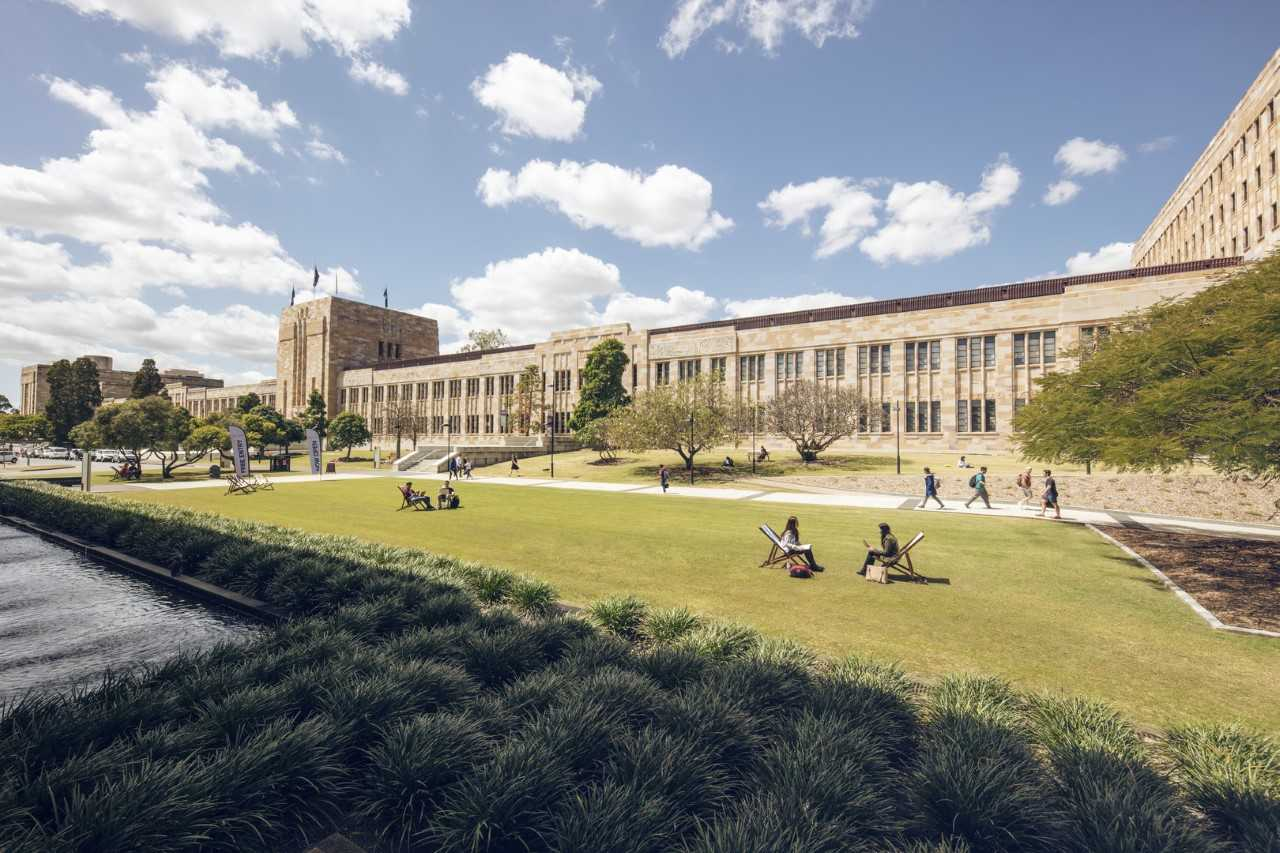
\includegraphics[width=1.0\textwidth]{Examples/FigureUQ}
\caption{The University Of Queensland}
\label{Fig:1}
\end{center}
\end{figure}

The Figure~\ref{Fig:1} represents beauty of the UQ campus.
%% ***************************************************
% Example of Flow Charts
% ***************************************************
%This example is provided for your reference only. DO NOT INCLUDE IN YOUR FINAL THESIS. 
\chapter{Example of Flow Charts}
\begin{figure}[h]
\caption{Flow Chart}
\label{Fig:FlowChart}
\begin{center}
\tikzstyle{decision} = [diamond, draw, fill=white!10, 
    text width=4.5em, text badly centered, node distance=3cm, inner sep=0pt]
\tikzstyle{block} = [rectangle, draw, fill=white!20, 
    text width=5em, text centered, rounded corners, minimum height=4em]
\tikzstyle{line} = [draw, -latex']
\tikzstyle{cloud} = [draw, ellipse,fill=white!20, node distance=3cm,
    minimum height=2em]
    
\begin{tikzpicture}[node distance = 2cm, auto]
    % Place nodes
    \node [block] (Step1) {initialize model};
    \node [cloud, left of=Step1] (expert) {expert};
    \node [cloud, right of=Step1] (system) {system};
    \node [block, below of=Step1] (identify) {identify candidate models};
    \node [block, below of=identify] (evaluate) {evaluate candidate models};
    \node [block, left of=evaluate, node distance=3cm] (update) {update model};
    \node [decision, below of=evaluate] (decide) {is best candidate better?};
    \node [block, below of=decide, node distance=3cm] (stop) {stop};
    % Draw edges
    \path [line] (Step1) -- (identify);
    \path [line] (identify) -- (evaluate);
    \path [line] (evaluate) -- (decide);
    \path [line] (decide) -| node [near start] {yes} (update);
    \path [line] (update) |- (identify);
    \path [line] (decide) -- node {no}(stop);
    \path [line,dashed] (expert) -- (Step1);
    \path [line,dashed] (system) -- (Step1);
    \path [line,dashed] (system) |- (evaluate);
\end{tikzpicture}
\end{center}
\end{figure}

Flow chart~\ref{Fig:FlowChart} is a simple example.
%% ***************************************************
% Example of Tables
% ***************************************************
%This example is provided for your reference only. DO NOT INCLUDE IN YOUR FINAL THESIS. 
\chapter{Example of Tables}

Here is a really simple table~\ref{Table}.


%\begin{table} : If you put no command after \begin{table} then this table will be printed anywhere in your pdf where LaTex finds the free space to put it. If you wish to specify where the table goes you have to give a command in LaTex after  \begin{table}. 
%
%There are different commands to put the table in different positions e.g. \begin{table}[h] LaTex will print the table in the same position that you put it in your source file, if there is enough space to print it
%N.B. it is important to note that commanding LaTeX to add a table in a specific place may result in formatting issues.

\begin{table}[h]
\caption{Name of the Australian Cities}
\begin{center}
\begin{tabular}{{|c|c|c|}}
\hline
\textbf{Number}& \textbf {Name}\\
\hline
      1& Brisbane\\
      2& Sydney\\
      3& Melbourne\\
      4& Canberra\\
      5& Perth\\
      6& Adelaide\\
      7& Hobart\\
      8& Darwin\\
\hline
\end{tabular}
\end{center}
\label{Table}
\end{table}


% ***************************************************
% Back Matter
%**************************************************** 
%COMMENT OUT IF YOU DO NOT WISH TO INCLUDE BACK MATTER.
%% ***************************************************
% Back Matter
% ***************************************************
% ADD AN ENDQUOTE HERE. If you do not wish to, delete this file.
\backmatter

\normalfont
\cleartooddpage

\pagestyle{empty}

\begin{table}[b!]
\begin{center}
% ********* Enter your quote within {} brackets: ********
\textit{Endquote goes here.}

% ********************************************************
\end{center}
\begin{flushright}
% ********* Enter your text below, as indicated: ********
Author of quote,\\
Source of quote

% ********************************************************
\end{flushright}
\end{table}

\end{document}
